\documentclass[UTF8,oneside,fontset=none]{ctexbook}

\usepackage{graphicx}
\usepackage{amsmath}
\usepackage{amssymb}
\usepackage{amsthm}
\usepackage{mathtools}
\usepackage{geometry}
\geometry{margin=1in}
\usepackage[unicode,bookmarks=false]{hyperref}
\usepackage{enumitem}
\usepackage{booktabs}
\usepackage{xcolor}
\usepackage{tikz}
\usepackage{float}
\usetikzlibrary{calc, decorations.pathreplacing, positioning}
\usepackage{microtype}
\usepackage[most]{tcolorbox}
\usepackage{xparse}
\allowdisplaybreaks

% CJK font settings with fallbacks.
% This avoids hard failure when a specific Noto/Source Han font is not installed.
% Compile with XeLaTeX.
\IfFontExistsTF{Source Han Serif SC}{
  \setCJKmainfont[AutoFakeBold=2, AutoFakeSlant=0.2]{Source Han Serif SC}
  \setCJKmonofont{Source Han Serif SC}
}{
  \IfFontExistsTF{SimSun}{
    \setCJKmainfont[AutoFakeBold=2, AutoFakeSlant=0.2]{SimSun}
    \setCJKmonofont{SimSun}
  }{
    \IfFontExistsTF{Noto Serif CJK SC}{
      \setCJKmainfont[AutoFakeBold=2, AutoFakeSlant=0.2]{Noto Serif CJK SC}
      \setCJKmonofont{Noto Serif CJK SC}
    }{
      \setCJKmainfont[AutoFakeBold=2, AutoFakeSlant=0.2]{FandolSong-Regular}
      \setCJKmonofont{FandolSong-Regular}
    }
  }
}

\IfFontExistsTF{Source Han Sans SC}{
  \setCJKsansfont[AutoFakeBold=2, AutoFakeSlant=0.2]{Source Han Sans SC}
}{
  \IfFontExistsTF{SimHei}{
    \setCJKsansfont[AutoFakeBold=2, AutoFakeSlant=0.2]{SimHei}
  }{
    \IfFontExistsTF{Noto Sans CJK SC}{
      \setCJKsansfont[AutoFakeBold=2, AutoFakeSlant=0.2]{Noto Sans CJK SC}
    }{
      \setCJKsansfont[AutoFakeBold=2, AutoFakeSlant=0.2]{FandolHei-Regular}
    }
  }
}

% Latin font fallbacks for XeLaTeX when fontset=none.
\IfFontExistsTF{TeX Gyre Termes}{
  \setmainfont{TeX Gyre Termes}
}{
  \IfFontExistsTF{Times New Roman}{
    \setmainfont{Times New Roman}
  }{
    \IfFontExistsTF{DejaVu Serif}{
      \setmainfont{DejaVu Serif}
    }{
      \setmainfont{Latin Modern Roman}
    }
  }
}

\IfFontExistsTF{TeX Gyre Heros}{
  \setsansfont{TeX Gyre Heros}
}{
  \IfFontExistsTF{Arial}{
    \setsansfont{Arial}
  }{
    \IfFontExistsTF{DejaVu Sans}{
      \setsansfont{DejaVu Sans}
    }{
      \setsansfont{Latin Modern Sans}
    }
  }
}

\IfFontExistsTF{Latin Modern Mono}{
  \setmonofont{Latin Modern Mono}
}{
  \IfFontExistsTF{Consolas}{
    \setmonofont{Consolas}
  }{
    \IfFontExistsTF{DejaVu Sans Mono}{
      \setmonofont{DejaVu Sans Mono}
    }{
      \setmonofont{Courier New}
    }
  }
}

\DeclareMathOperator{\arcsec}{arcsec}
\DeclareMathOperator{\arccot}{arccot}
\DeclareMathOperator{\arccsc}{arccsc}
\DeclareMathOperator{\sech}{sech}
\DeclareMathOperator{\csch}{csch}
\DeclareMathOperator{\arcsinh}{arcsinh}
\DeclareMathOperator{\arccosh}{arccosh}
\DeclareMathOperator{\arctanh}{arctanh}

% Colorful Environments for Theorems, Definitions, etc.
\newtcbtheorem[number within=section]{mydef}{定义}{
        enhanced,
        breakable,
        colback=blue!5!white,
        colframe=blue!75!black,
        attach boxed title to top left={yshift*=-\tcboxedtitleheight/2},
        fonttitle=\bfseries,
        boxed title style={colback=blue!75!black, colframe=blue!75!black}
}{def}

\newtcbtheorem[number within=section]{mythm}{定理}{
        enhanced,
        breakable,
        colback=red!5!white,
        colframe=red!75!black,
        attach boxed title to top left={yshift*=-\tcboxedtitleheight/2},
        fonttitle=\bfseries,
        boxed title style={colback=red!75!black, colframe=red!75!black}
}{thm}

\newtcbtheorem[number within=section]{myproposition}{命题}{
        enhanced,
        breakable,
        colback=orange!5!white,
        colframe=orange!80!black,
        attach boxed title to top left={yshift*=-\tcboxedtitleheight/2},
        fonttitle=\bfseries,
        boxed title style={colback=orange!80!black, colframe=orange!80!black}
}{prp}

\newtcbtheorem[number within=section]{myprop}{性质}{
        enhanced,
        breakable,
        colback=green!5!white,
        colframe=green!60!black,
        attach boxed title to top left={yshift*=-\tcboxedtitleheight/2},
        fonttitle=\bfseries,
        boxed title style={colback=green!60!black, colframe=green!60!black}
}{prop}

\newtcbtheorem[number within=section]{mycor}{推论}{
        enhanced,
        breakable,
        colback=violet!5!white,
        colframe=violet!75!black,
        attach boxed title to top left={yshift*=-\tcboxedtitleheight/2},
        fonttitle=\bfseries,
        boxed title style={colback=violet!75!black, colframe=violet!75!black}
}{cor}

\newtcbtheorem[number within=section]{myex}{例}{
        enhanced,
        breakable,
        colback=teal!5!white,
        colframe=teal!75!black,
        attach boxed title to top left={yshift*=-\tcboxedtitleheight/2},
        fonttitle=\bfseries,
        boxed title style={colback=teal!75!black, colframe=teal!75!black}
}{ex}

\newtcbtheorem[number within=section]{myrem}{注记}{
        enhanced,
        breakable,
        colback=gray!5!white,
        colframe=gray!75!black,
        attach boxed title to top left={yshift*=-\tcboxedtitleheight/2},
        fonttitle=\bfseries,
        boxed title style={colback=gray!75!black, colframe=gray!75!black}
}{rem}

\newtcolorbox{mynote}{
        enhanced,
        breakable,
        colback=yellow!10!white,
        colframe=orange!85!black,
        title={\textbf{注}},
        coltitle=black,
        attach boxed title to top left={yshift*=-\tcboxedtitleheight/2},
        boxed title style={colback=orange!50!yellow, colframe=orange!85!black},
        sharp corners=south,
}

% Environment Mappings
\theoremstyle{definition}
\newtheorem{definition}{定义}[section]

\ProvideDocumentEnvironment{theorem}{o}
    {\IfValueTF{#1}{\begin{mythm}{#1}{}}{\begin{mythm}{}{}}}
    {\end{mythm}}

\ProvideDocumentEnvironment{proposition}{o}
    {\IfValueTF{#1}{\begin{myproposition}{#1}{}}{\begin{myproposition}{}{}}}
    {\end{myproposition}}

\ProvideDocumentEnvironment{property}{o}
    {\IfValueTF{#1}{\begin{myprop}{#1}{}}{\begin{myprop}{}{}}}
    {\end{myprop}}

\ProvideDocumentEnvironment{corollary}{o}
    {\IfValueTF{#1}{\begin{mycor}{#1}{}}{\begin{mycor}{}{}}}
    {\end{mycor}}

\ProvideDocumentEnvironment{inference}{o}
    {\IfValueTF{#1}{\begin{mycor}{#1}{}}{\begin{mycor}{}{}}}
    {\end{mycor}}

\ProvideDocumentEnvironment{example}{o}
    {\IfValueTF{#1}{\begin{myex}{#1}{}}{\begin{myex}{}{}}}
    {\end{myex}}

\ProvideDocumentEnvironment{remark}{o}
    {\IfValueTF{#1}{\begin{myrem}{#1}{}}{\begin{myrem}{}{}}}
    {\end{myrem}}

\ProvideDocumentEnvironment{note}{}{\begin{mynote}}{\end{mynote}}

\ProvideDocumentEnvironment{lemma}{o}
    {\IfValueTF{#1}{\begin{mythm}{#1}{}}{\begin{mythm}{}{}}}
    {\end{mythm}}

\newcommand{\prefacechapter}{%
  \cleardoublepage
  \chapter*{序言}
  \addcontentsline{toc}{chapter}{序言}
}

\newcommand{\chapterzero}{%
  \cleardoublepage
  \chapter*{第 0 章：基础知识与记号}
  \addcontentsline{toc}{chapter}{第 0 章：基础知识与记号}
  \setcounter{section}{0}
  \renewcommand{\thesection}{0.\arabic{section}}
}

\begin{document}


\begin{titlepage}
\newgeometry{margin=0pt}
\thispagestyle{empty}

\definecolor{covercream}{RGB}{239,226,205}
\definecolor{covermuted}{RGB}{205,211,220}
\definecolor{covernight}{RGB}{9,22,39}
\definecolor{covergold}{RGB}{232,196,143}

\begin{tikzpicture}[remember picture, overlay]
    % Full-bleed cover image. The image is the new photo supplied by the user.
    \node[inner sep=0pt] at (current page.center)
        {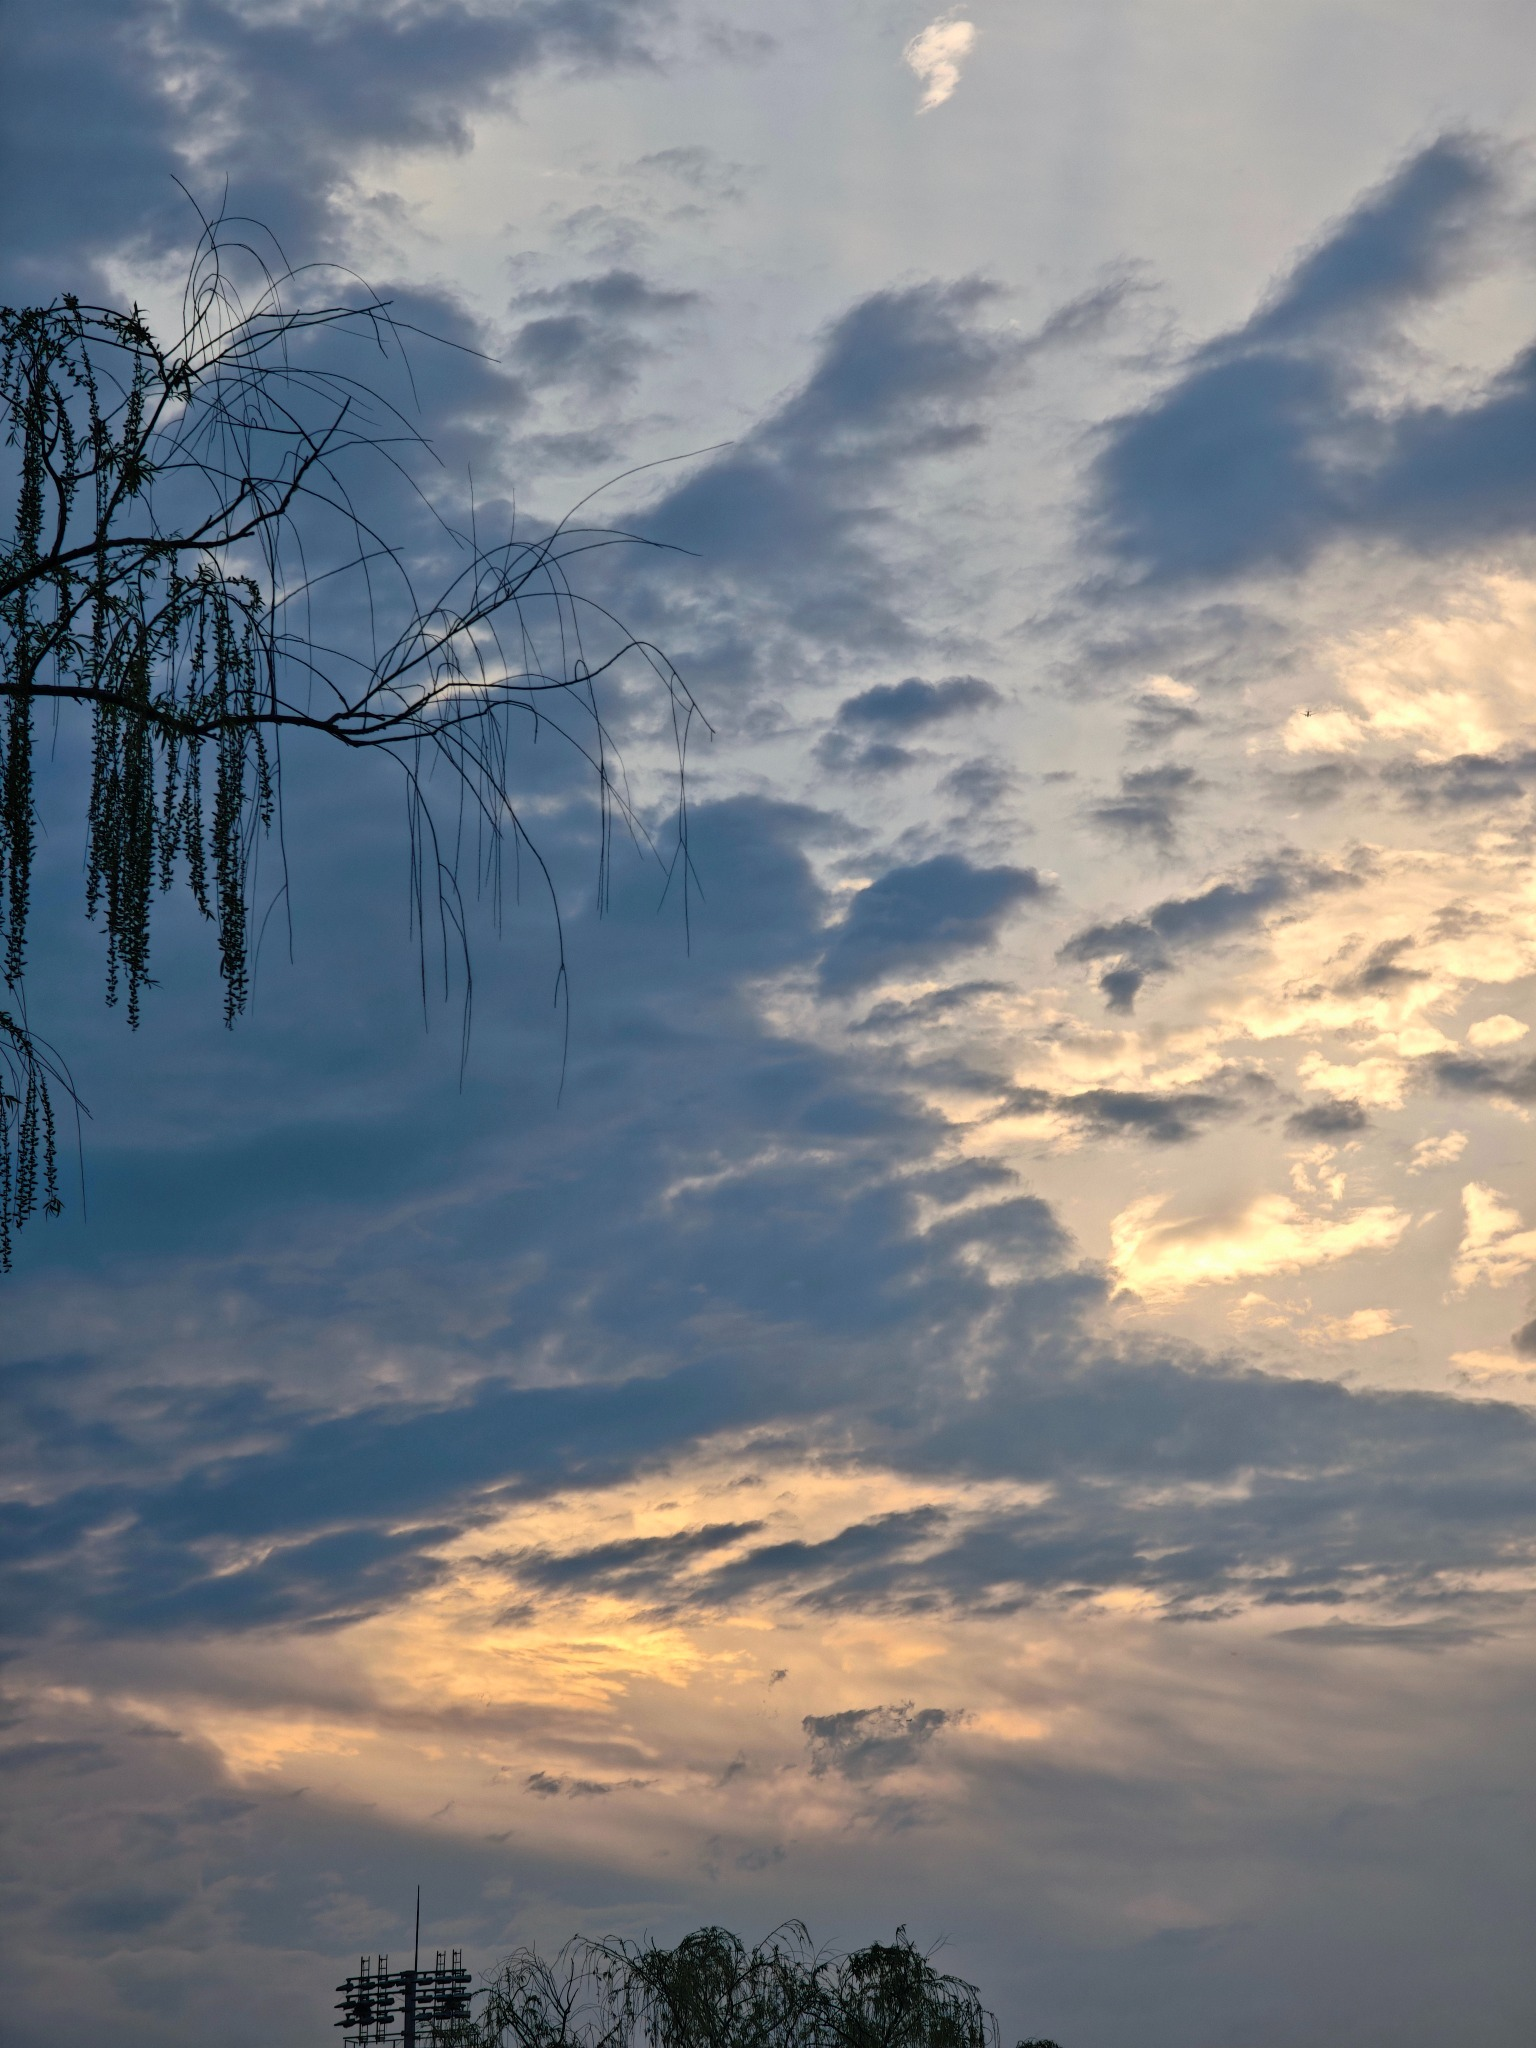
\includegraphics[width=\paperwidth,height=\paperheight]{assets/cover_sky.jpg}};

    % Quiet editorial overlays: keep the sky visible but give the type enough contrast.
    \fill[covernight, opacity=0.50] (current page.south west) rectangle (current page.north east);

    % Main Chinese title: serif-first, restrained, with generous negative space.
    \node[anchor=north west, inner sep=0pt, text=covercream]
        at ($(current page.north west)+(0.82in,-1.35in)$) {%
        \begin{minipage}{0.72\paperwidth}
            {\rmfamily\fontsize{34}{46}\selectfont\bfseries 数学与公理化}\par
            \vspace{0.33in}
            {\color{covercream!74}\rule{0.46\paperwidth}{0.45pt}}\par
            \vspace{0.20in}
            {\rmfamily\fontsize{14.5}{24}\selectfont\color{covercream!95} 数\quad 学\quad 笔\quad 记}\par
            \vspace{0.06in}
            {\rmfamily\fontsize{7.3}{12}\selectfont\color{covermuted!88}
            M\,A\,T\,H\,E\,M\,A\,T\,I\,C\,S\quad N\,O\,T\,E\,S}\par
        \end{minipage}
    };

    % Author block.
    \draw[covercream!72, line width=0.7pt]
        ($(current page.south west)+(0.83in,1.02in)$) -- ++(0,0.56in);
    \node[anchor=south west, align=left, text=covercream!94, inner sep=0pt]
        at ($(current page.south west)+(1.02in,0.86in)$)
        {\rmfamily\fontsize{13.5}{21}\selectfont\bfseries 李谨硕\\[0.13in]
        \rmfamily\fontsize{9.6}{15}\selectfont\color{covermuted!93}上海交通大学\\[0.08in]
        \rmfamily\fontsize{8.8}{14}\selectfont\color{covercream!86}2026.7.2，于上海};

    % Bottom motto in Chinese to make the cover feel native rather than translated.
    \node[anchor=south, text=covercream!62, inner sep=0pt]
        at ($(current page.south)+(0,0.52in)$)
        {\rmfamily\fontsize{7.8}{13}\selectfont 探\,索\quad ·\quad 思\,考\quad ·\quad 理\,解};
\end{tikzpicture}
\end{titlepage}
\restoregeometry
\thispagestyle{empty}

\cleardoublepage
\pagenumbering{gobble}
\tableofcontents
\thispagestyle{empty}

% perface.tex
% 序言中文译稿。文件名按用户要求保留为 perface.tex。

\prefacechapter

数学的核心处存在着一种美丽而根本的张力：一方面，是人类对世界与生俱来的直观把握；另一方面，是数学对绝对确定性毫不妥协的要求。

每个人最开始都是一名朴素的数学家。我们观察模式，感受关系，并且带着一种本能的自信去操作数字和图形。这种“朴素理解”是所有数学好奇心生长的土壤。它自然、有力，并且深深地具有人类自身的特征。

然而，历史已经表明，当直觉被推到自身边界之外时，它也可能成为一种危险的向导，带来矛盾与不确定性。因此，现代数学这座宏伟的大厦不能仅仅建立在这片土壤之上。它还需要把地基深深打入逻辑严密性的基岩之中。

从最简单的细节开始，经过数百代人的努力，数学家不断抽象数学概念，并建立起一座逻辑的大厦。几何学家从最基本的几何结构——点、线、面——开始，通过严谨的公设和证明建立了欧几里得平面几何体系。这个基础框架强调全等、相似以及空间性质，后来逐渐发展并扩展为现代高等几何。在这一过程中，非欧几何挑战了人们长期以来关于平行线和曲率的假设。进一步地，它又发展出拓扑学，即研究在连续变形下保持不变的形状与空间的学科，并且还催生了流形等概念，为物理学以及更高维现实的理解提供了数学支架。

与此同时，代数学家从最根本的概念——数量本身——出发，围绕加法、减法以及解未知数方程等运算，建立起简单而初等的代数。随着时间推移，他们进一步抽象出代数结构，认识到群、环、域中的模式，由此发展出线性代数等学科。线性代数刻画向量空间和变换，是从计算机图形学到量子力学等领域不可或缺的工具；而今天所说的抽象代数，则进入了纯粹结构的领域，并支撑着密码学、编码理论以及宇宙中的对称性研究。

这种抽象过程也延伸到了其他分支。在分析学中，学者们从极限和连续性的直观观念出发，将其形式化为 Newton 和 Leibniz 的严密微积分体系，随后又发展为实分析、复分析、测度论和泛函分析。这些工具使我们能够处理无穷、概率以及无限维空间中函数的行为。数论学家则从人类对整数和素数的原初兴趣出发，构造出各种算术体系，并逐渐分化出解析数论、代数数论，甚至通向 Riemann 猜想这样深刻的谜题，把素数与复函数的零点联系起来。

本书讨论的正是这座大厦的建造过程。它讲述的是从直观这片肥沃但模糊的土地，走向形式化公理系统那种晶体般清晰结构的旅程。我们将看到，数学家如何经过数百年的智力劳动，把他们的直觉想法提炼为精确的定义和明确无歧义的规则——也就是公理。

这些公理是数学摩天大楼的基石。经过谨慎选择之后，它们既足够简单，看起来近乎自明；又足够强大，可以支撑起一座不断向上延伸的思想高塔。每一层新的结构——一个定理、一套理论，甚至像微积分或代数这样的一整门新学科——都稳固地建造在其下方的层级之上，而它的可靠性则由连接它与基础的逻辑关系来保证。

正是这种建筑原则，使数学成为所有语言中最具统一性的语言。它把图形的几何世界与方程的代数世界联系起来，把整数的离散世界与分析的连续世界联系起来，并把它们编织成一个单一、宏大而连贯的叙事。它连接统计学中的概率不确定性与逻辑中的确定性，甚至还把集合论这样的抽象领域——在其中无穷被驯服、悖论被化解——与计算机科学和工程等应用领域联系起来。

这座摩天大楼见证了人类理性的力量。然而，Gödel 不完备定理也为它投下了一道迷人且必要的阴影。它提醒我们，即使是最完美建造的摩天大楼，也无法在自身内部拥有工具来验证其最深层地基的稳定性。这并不是一种会使结构崩塌的缺陷；相反，它揭示了这座结构本身的深刻本质。

它告诉我们，数学并不是一座静止的、已经完成的绝对真理神殿，而是一场活着的、不断生长的、永远令人着迷的人类冒险。无法获得一个最终的、自我验证的系统，并不是一种弱点，而是一种力量的来源——它保证了这场冒险永远不会终结，保证了总会有新的地平线等待探索，也总会有新的问题等待提出。它邀请我们拥抱未知，推动我们所能形式化的边界，并在确定性与神秘性之间的相互作用中发现美。

这份手稿就是一份加入这场伟大冒险的邀请。它面向的读者，并不是只满足于被告知一个结论的人；它更适合那些希望站在设计图前，按照逻辑的步骤，一步一步理解这座摩天大楼如何被设计并建造起来的人。在这个过程中，我们会遇到发现的胜利，也会遇到早期误解所带来的陷阱，还会看到那些优雅的解决方式如何塑造出今天的数学。

每掌握一个新的概念，从这座摩天大楼上看到的景色就会更加壮丽。

欢迎你。


\cleardoublepage
\pagenumbering{arabic}
\setcounter{page}{1}

% chapter0_cn.tex
% 第 0 章中文译稿。

\chapterzero

所有数学洞见都会经历一个从“朴素理解”到“严谨表述”的过程。数学自身也是如此；一切公理化语言都无法完全脱离经验主义者的朴素描述性语言。

为了介绍今后会频繁使用的一些特殊数学符号，我特意在第一章之前加入了第零章，用来呈现关于数学语言和数学逻辑的部分知识。在本章中，我也会介绍一些与公理有关的内容；不过在后续章节中，我们不一定每次都如此严格地定义公理。

\section{命题逻辑}

\subsection{命题逻辑的朴素引入}

在正式进入命题逻辑的主要内容之前，先从一个问题开始：什么是命题？请看下面这些句子：

\begin{enumerate}
    \item 方程 $x^2+1=0$ 有实数解；
    \item 素数有无穷多个；
    \item 每一个不小于 $4$ 的偶整数 $n$ 都可以写成两个素数之和，也就是著名的 Goldbach 猜想；
    \item 现在几点了？
    \item 这句话是假的。
\end{enumerate}

在上面的句子中，前三个句子具有相同的性质：一是它们都是陈述事实的句子或断言；二是它们要么为真，要么为假，但不能同时既真又假。然而，第四个句子不是陈述句，而第五个句子的正确性无法判定。

所以，为了研究数学，我们需要那些断言一个或若干事实的句子。有时候，只要它的真值能够被确定，它究竟是真是假并不是最重要的。这并不意味着其他类型的表达不重要。我们之所以重视这类表达，是因为所有公理、定义和定理都是以这种形式写成的。

\begin{definition}[命题]
命题是陈述事实的句子或断言，并且它要么为真，要么为假，但不能同时既真又假。
\end{definition}

为了让命题更便于操作，我们使用\textbf{命题变量}来表示不同的命题。常用的命题变量包括 $p,q,r,\dots$ 等字母。

有时我们需要把不同的命题变量连接起来，形成新的命题。这时就需要使用“并且”“或者”“推出”等词语来说明它们之间的关系。

\begin{definition}[逻辑运算符/逻辑联结词]
逻辑运算符或逻辑联结词，是用来连接命题变量并形成复合命题的符号。
\end{definition}

常见的逻辑运算符如下：

\begin{itemize}
    \item $\neg$：否定，即“非”。
    \item $\wedge$：合取，即“并且”。
    \item $\vee$：析取，即“或者”。
    \item $\to$ 或 $\Rightarrow$：条件，即“推出”。
    \item $\leftrightarrow$：双条件，即“当且仅当”。
    \item $\oplus$：异或。
\end{itemize}

\begin{definition}[复合命题]
复合命题是由命题变量或命题常量通过逻辑运算符构造出来的命题。
\end{definition}

\begin{definition}[原子命题]
原子命题是不能再进一步分解的命题。它是逻辑表达式中最基本的构成单位，并被看作一个不可再分的语义单位。
\end{definition}

如果要判断一个原子命题是否为真，我们需要使用数学不同领域中的相关知识。但怎样判断一个复合命题的真假呢？我们可以使用真值表。

\begin{definition}[真值表]
真值表是逻辑中使用的一种数学表格，用于根据输入值计算逻辑表达式的真值。
\end{definition}

\paragraph{否定}
\[
\begin{array}{c|c}
p & \neg p \\
\hline
T & F \\
F & T
\end{array}
\]

\paragraph{合取}
\[
\begin{array}{c|c|c}
p & q & p\wedge q \\
\hline
T & T & T \\
T & F & F \\
F & T & F \\
F & F & F
\end{array}
\]

\paragraph{析取}
\[
\begin{array}{c|c|c}
p & q & p\vee q \\
\hline
T & T & T \\
T & F & T \\
F & T & T \\
F & F & F
\end{array}
\]

\paragraph{条件，即蕴含}
\[
\begin{array}{c|c|c}
p & q & p\to q \\
\hline
T & T & T \\
T & F & F \\
F & T & T \\
F & F & T
\end{array}
\]

\paragraph{双条件，即当且仅当}
\[
\begin{array}{c|c|c}
p & q & p\leftrightarrow q \\
\hline
T & T & T \\
T & F & F \\
F & T & F \\
F & F & T
\end{array}
\]

\paragraph{异或}
\[
\begin{array}{c|c|c}
p & q & p\oplus q \\
\hline
T & T & F \\
T & F & T \\
F & T & T \\
F & F & F
\end{array}
\]

就像数值计算一样，逻辑运算符也有优先级。下面是逻辑运算符从高到低的优先级顺序：
\[
( ), [ ] \quad \neg \quad \wedge \quad \vee \quad \oplus \quad \to \quad \leftrightarrow.
\]
除此之外，先出现的运算符具有更高的优先级。简而言之，我们先计算优先级较高的逻辑运算符，再计算优先级较低的运算符。

利用这些规则，我们可以定义不同命题的真值。不过，复合命题中还存在一些特殊类别：

\begin{itemize}
    \item \textbf{重言式}：无论命题变量取什么真值，始终为真的复合命题。
    \item \textbf{矛盾式}：无论命题变量取什么真值，始终为假的复合命题。
    \item \textbf{偶然式}：既不是重言式，也不是矛盾式的复合命题。它可以为真，也可以为假，取决于变量的取值。
\end{itemize}

基于上面的定义，现在可以严格定义什么是逻辑等价。

\begin{definition}[逻辑等价]
如果 $p\leftrightarrow q$ 是一个重言式，那么我们称复合命题 $p,q$ \textbf{逻辑等价}。如果 $p$ 和 $q$ 逻辑等价，记作
\[
p\equiv q.
\]
\end{definition}

这个定义的意思是：对于每一个原子命题的不同真值组合，$p$ 和 $q$ 最终得到的真值都相同。在后续学习中，我们会知道，上面这些运算符中的若干个就已经足够表达所有命题。

下面列出一些经常使用的例子。这些等价式可以直接使用：
\begin{align*}
\text{恒等律：}\quad & p\wedge T\equiv p, & p\vee F\equiv p; \\
\text{支配律：}\quad & p\vee T\equiv T, & p\wedge F\equiv F; \\
\text{吸收律：}\quad & p\vee(p\wedge q)\equiv p, & p\wedge(p\vee q)\equiv p; \\
\text{否定律：}\quad & p\vee\neg p\equiv T, & p\wedge\neg p\equiv F; \\
\text{交换律：}\quad & p\vee q\equiv q\vee p, & p\wedge q\equiv q\wedge p; \\
\text{结合律：}\quad & (p\vee q)\vee r\equiv p\vee(q\vee r), & (p\wedge q)\wedge r\equiv p\wedge(q\wedge r); \\
\text{分配律：}\quad & p\vee(q\wedge r)\equiv(p\vee q)\wedge(p\vee r), & p\wedge(q\vee r)\equiv(p\wedge q)\vee(p\wedge r); \\
\text{德摩根律：}\quad & \neg(p\wedge q)\equiv\neg p\vee\neg q, & \neg(p\vee q)\equiv\neg p\wedge\neg q.
\end{align*}

\begin{definition}[可满足性]
如果一个复合命题在某种命题变量的真值赋值下为真，那么称它是\textbf{可满足的}。能够使复合命题为真的真值赋值称为一个\textbf{解}。如果一个复合命题不可满足，我们称它是\textbf{不可满足的}。
\end{definition}

目前，我们可以使用真值表和逻辑等价来检查一个复合命题是否可满足。对于计算机科学专业的读者，也可以使用专门的算法来解决所谓的“布尔可满足性问题”，例如启发式搜索等。

\subsection{功能完备性}

根据前面的学习，我们知道不同变量之间可以通过联结词构成复合命题。然而，我们真的需要这么多联结词来表示所有关系和所有复合命题吗？答案显然是否定的。在某些情况下，我们只需要两个联结词就可以达到所谓的功能完备状态。

\begin{definition}[析取范式]
如果一个复合命题是若干个合取项的析取，并且这些合取项由命题变量或它们的否定构成，那么称该复合命题处于\textbf{析取范式}，英文为 \textbf{disjunctive normal form，DNF}。
\end{definition}

\begin{theorem}
每一个复合命题都逻辑等价于某个析取范式形式的复合命题。
\end{theorem}

\begin{proof}
这个定理并不难证明。根据前面的内容，我们知道每一个复合命题都可以写出真值表。根据真值表，我们可以把它改写成析取范式。例如，异或联结词的真值表为：
\[
\begin{array}{c|c|c}
p & q & p\oplus q \\
\hline
T & T & F \\
T & F & T \\
F & T & T \\
F & F & F
\end{array}
\]
中间两行，也就是结果为 $T$ 的两行，表示这个复合命题的解。因此，我们可以写出如下命题：
\[
p\oplus q\equiv(p\wedge\neg q)\vee(\neg p\wedge q).
\]
这个复合命题中，每一个由析取连接起来的部分都表示原命题可满足性问题的一个解。这说明，只要能够为复合命题写出真值表，就可以把它改写成析取范式。从这个角度看，定理是相当清楚的。
\end{proof}

进一步来看：我们能否把复合命题改写成其他形式？答案显然也是可以的。

\begin{definition}[合取范式]
如果一个复合命题是若干个析取项的合取，并且这些析取项由命题变量或它们的否定构成，那么称该复合命题处于\textbf{合取范式}，英文为 \textbf{conjunctive normal form，CNF}。
\end{definition}

\begin{theorem}
每一个复合命题都逻辑等价于某个合取范式形式的复合命题。
\end{theorem}

\begin{proof}
我们仍然使用真值表来证明这个定理。设有一个命题 $A$。首先，利用定理 0.1.1，把 $\neg A$ 改写为析取范式。接下来，对 $\neg A$ 再取否定，并使用德摩根律，就可以把 $A$ 改写为合取范式。
\end{proof}

定理 0.1.1 和定理 0.1.2 非常巧妙。在电路设计中，由于我们不可能为每一个逻辑联结词都设计一个电路元件，所以必须使用尽可能少的电路元件来表达所有逻辑表达式。根据这些定理，我们不再需要使用那么多联结词。只需要合取、析取和否定，就足以构造出与世界上任意命题逻辑等价的命题。

\begin{definition}[功能完备]
如果任意复合命题都逻辑等价于某个只使用某一逻辑运算符集合中运算符的复合命题，那么称这个逻辑运算符集合是\textbf{功能完备的}。
\end{definition}

因此，我们可以说集合
\[
\{\neg,\vee,\wedge\}
\]
是功能完备的。同时，根据德摩根律：
\[
p\wedge q\equiv\neg(\neg p\vee\neg q),
\]
\[
p\vee q\equiv\neg(\neg p\wedge\neg q),
\]
可以发现，合取可以用析取和否定表示，而析取也可以用合取和否定表示。这意味着集合
\[
\{\neg,\vee\}
\]
和
\[
\{\neg,\wedge\}
\]
也是功能完备的。

\begin{note}
最令人惊讶的事实是，确实存在一种联结词，它本身就是功能完备的，例如 NAND 或 NOR。不过我们以后不会使用它，所以读者可以自行查阅。
\end{note}

\section{谓词逻辑}

在很多情况下，使用命题逻辑已经足够。但有一类陈述无法用命题逻辑工具表达。在这种情况下，我们需要使用谓词逻辑来构造逻辑表达式。

\begin{definition}[谓词]
\textbf{谓词}是一种带有变量的陈述。谓词也称为\textbf{命题函数}。谓词可以记作
\[
P(x,y,z,\dots),
\]
其中 $x,y,z$ 称为变量。
\end{definition}

\begin{definition}[量词]
我们使用\textbf{量词}来表示所涉及元素的数量。量词有两类：$\forall$ 和 $\exists$。
\begin{itemize}
    \item $\forall$：\textbf{全称量词}，意思是“对所有”或“任意”。
    \item $\exists$：\textbf{存在量词}，意思是“存在”。
\end{itemize}
\end{definition}

例如，“每一位 SJTUer 都是人才”这个陈述可以写成谓词逻辑的形式：
\[
\forall x(\text{SJTUer}(x)\to \text{Talent}(x)).
\]

谓词中的变量都有受限制的取值范围，这些范围称为谓词的\textbf{论域}。对于论域中的所有值，我们都可以把谓词改写为命题的形式。如果论域是有限集合
\[
\{x_1,x_2,\dots,x_n\},
\]
那么有：
\[
\forall x P(x)\equiv P(x_1)\wedge P(x_2)\wedge\dots\wedge P(x_n),
\]
\[
\exists x P(x)\equiv P(x_1)\vee P(x_2)\vee\dots\vee P(x_n).
\]
但如果论域是无限的，我们就只能用谓词逻辑的形式来表达这种逻辑关系。

\begin{itemize}
    \item $\forall xP(x)$ 表示“对于论域中的每一个 $x$，$P(x)$ 都成立”。如果论域中存在某个值 $a$，使得 $P(a)$ 为假，那么这个陈述就是假的。这个 $a$ 称为一个\textbf{反例}。
    \item $\exists xP(x)$ 表示“存在一个 $x$，使得 $P(x)$ 成立”。如果对于论域中所有值 $a$，$P(a)$ 都为假，那么这个陈述就是假的。
\end{itemize}

然而，并不是所有带有谓词和量词的句子都能形成谓词逻辑中的命题。例如，
\[
\forall x(P(x)\wedge Q(y))
\]
就不是一个完整的谓词逻辑命题。因为当 $y$ 的取值发生变化时，我们无法判断这个句子是真的还是假的，因此它的真值是不确定的。

那么，怎样才能确保一个句子是谓词逻辑中的命题呢？在
\[
\forall x(P(x)\wedge Q(y))
\]
这个例子中，造成问题的是 $y$。而与量词相连的 $x$ 并没有造成不便。因此，我们称那些跟在量词之后并受到量词约束的变量为\textbf{约束变量}；否则，它们就是\textbf{自由变量}。如果一个句子中的每一个变量都是约束变量，那么它就是一个命题。

和命题逻辑一样，谓词逻辑中的表达式也可以用逻辑联结词连接，并且也有一些运算规律。

\paragraph{量词的德摩根律}
\[
\neg\forall xP(x)\equiv\exists x\neg P(x),
\]
\[
\neg\exists xP(x)\equiv\forall x\neg P(x).
\]

\paragraph{非对称结合律}
\[
\forall x\forall yP(x,y)\equiv\forall y\forall xP(x,y),
\]
\[
\exists x\exists yP(x,y)\equiv\exists y\exists xP(x,y).
\]

\begin{note}
这里的结合规律是非对称的。下面两个断言不一定成立。在某些情况下，它们甚至可能是假的：
\[
\forall x\exists yP(x,y)\not\equiv\exists y\forall xP(x,y).
\]
\end{note}

\begin{definition}[谓词逻辑中的逻辑等价]
如果 $\phi$ 和 $\psi$ 是带有谓词和量词、但没有自由变量的陈述，那么我们称 $\phi$ 和 $\psi$ \textbf{逻辑等价}，记作
\[
\phi\equiv\psi,
\]
其含义是：无论给定怎样的具体谓词，也无论给定怎样的论域，$\phi$ 和 $\psi$ 的真值总是一致的。
\end{definition}

此外，我们也可以定义普遍有效性，类似于命题逻辑中的重言式；谓词逻辑中也存在可满足性。由于本章只是一个简要介绍，因此这里不再进一步展开。

在本章中，我们初步认识了数学形式下的逻辑。关于命题逻辑和谓词逻辑的这个概览，为清晰推理建立了形式基础。逻辑是理性思维不可或缺的脚手架，是先于一切具体知识的\textbf{先验框架}。它的重要性不需要再作过多说明。

\noindent
\textbf{关键词：} 命题逻辑，谓词逻辑，逻辑等价。\\
\textbf{参考文献：} Kenneth H. Rosen, \textit{Discrete Mathematics and Its Applications}, Eighth Edition, McGraw-Hill Education.


\renewcommand{\thesection}{\arabic{chapter}.\arabic{section}}
% chapter1_cn.tex
% 第 1 章中文译稿。
\chapter{一切分支的公理}
\renewcommand{\thesection}{\arabic{chapter}.\arabic{section}}

在现代数学中，是否存在某一个单一的公理系统，可以称为“所有数学分支的公理”？这是一个相当微妙的问题，因为不同领域的研究者对此会给出不同答案。不过，如果取多数答案的交集，我们大概只会在这个集合中发现一个元素：集合论。

\section{朴素集合论}

实际上，如果你是工程类或应用数学方向的学生，学习朴素集合论通常已经足够覆盖学习和工作中需要的大部分数学内容。不过需要知道，朴素集合论本质上是一种直观定义，它并不是现代公理化集合论的一部分。虽然朴素集合论对于“集合”这个概念给出了非常清楚且实用的描述，但仍然必须说明，朴素集合论是不完备的，因为它本身无法解决 Russell 悖论。后文会向读者介绍这个引发第三次数学危机的悖论。

\begin{definition}[集合]
\textbf{集合}是由互不相同的对象组成的无序汇集，这些对象称为集合的\textbf{元素}或\textbf{成员}。我们说一个集合\emph{包含}它的元素。记号 $a \in A$ 表示 $a$ 是集合 $A$ 的一个元素；记号 $a \notin A$ 表示 $a$ 不是该集合的元素。
\end{definition}

集合的概念相当简单。集合可以作为任何对象的容器，比如数字、点、其他集合，甚至一个苹果也可以被看作集合。唯一的要求是，集合中的元素必须互不相同。例如，集合 $\{1,2,2,3\}$ 实际上等于集合 $\{1,2,3\}$，因为元素 $2$ 被重复写出了。

\begin{note}
一个对象只能处于两种状态之一：要么“属于 $A$”，要么“不属于 $A$”。它不能同时处于这两种状态，也不能两种状态都不处于。
\end{note}

\begin{definition}[子集]
如果集合 $A$ 的每一个元素都是集合 $B$ 的元素，那么称 $A$ 是 $B$ 的\textbf{子集}，记作 $A \subseteq B$。此外，如果 $A \subseteq B$ 且 $A \ne B$，那么称 $A$ 是 $B$ 的\textbf{真子集}，记作 $A \subset B$。
\end{definition}

子集的概念也很直观。如果集合 $A$ 中的所有元素都能在集合 $B$ 中找到，那么 $A$ 就是 $B$ 的子集。例如，$\{1,2\}\subseteq \{1,2,3\}$，并且 $\{1,2\}\subset \{1,2,3\}$。不过，在后续学习中我们会看到，子集这一概念在朴素集合论中会造成矛盾，而这正是 Russell 悖论的根源。

\begin{definition}[相等]
如果两个集合 $A$ 和 $B$ 包含完全相同的成员，那么称它们\textbf{相等}，也就是说它们是同一个集合，记作 $A=B$。
\end{definition}

集合相等可以通过子集的定义来判定。如果 $A \subseteq B$ 且 $B \subseteq A$，那么 $A=B$。这就是集合相等的形式化定义。

下面列出几个常见的集合运算。

\begin{definition}[集合并]
集合 $A$ 与 $B$ 的\textbf{并集}记作 $A\cup B$，它包含 $A$ 的所有元素以及 $B$ 的所有元素。
\end{definition}

\begin{definition}[集合交]
集合 $A$ 与 $B$ 的\textbf{交集}记作 $A\cap B$，它包含那些同时属于 $A$ 和 $B$ 的元素。
\end{definition}

\begin{definition}[集合差]
集合 $A$ 关于 $B$ 的\textbf{差集}记作 $A-B$，也可写作 $A\setminus B$。它由那些属于 $A$ 但不属于 $B$ 的元素组成。
\end{definition}

\begin{definition}[空集]
\textbf{空集}记作 $\emptyset$，是一个不包含任何元素的集合。
\end{definition}

注意，空集是任意集合的子集。而且，在整个集合宇宙中只有一个空集。这意味着，如果两个集合都没有元素，那么它们相等。

\begin{definition}[幂集]
集合 $x$ 的\textbf{幂集} $\mathcal{P}(x)$，也记作 $2^x$，是由 $x$ 的所有子集构成的集合。
\end{definition}

根据以上定义，我们很容易得到下面几个结论：

\begin{inference}
\begin{enumerate}
\item 对任意集合 $A$，都有 $\emptyset \subseteq A$。

\item 如果有限集合 $x$ 的元素个数为 $\text{card}(x)$，那么
$\text{card}(\mathcal{P}(x))=2^{\text{card}(x)}$。

\item 如果集合 $x$ 为空集，那么 $\text{card}(\mathcal{P}(\emptyset))=1$。这一推论可以看作推论 1.1.2 的延伸。
\end{enumerate}
\end{inference}

\subsection*{Russell 悖论}

Russell 悖论说明了朴素集合论的不完备性。Russell 假设存在一个集合 $X$，它包含所有“不包含自身的集合”：
\[
X=\{x\mid x\notin x\}.
\]
随后他发现，$X$ 既不能属于集合 $X$，也不能不属于集合 $X$。具体来说，
\begin{align*}
    X\in X &\implies X\notin X,\\
    X\notin X &\implies X\in X.
\end{align*}

那么，$X$ 到底是否属于 $X$ 呢？这就造成了矛盾。因为按照朴素集合论自身的性质，$X$ 要么属于 $X$，要么不属于 $X$。然而，朴素集合论的性质又允许集合 $X$ 的存在，于是矛盾就出现了。

为了修补朴素集合论中的这一缺陷，无数数学家投入了大量努力，并提出了 ZFC 公理系统。这个系统最终成为现代集合论的核心。

\section{公理化集合论}

\subsection{ZFC 公理系统}

ZFC 是 \textbf{Zermelo--Fraenkel Set Theory with the Axiom of Choice} 的缩写，即“带选择公理的 Zermelo--Fraenkel 集合论”。它包含九条不同的公理，编号为 ZF1 到 ZF8，以及 AC。下面逐一介绍。

\paragraph{基本原则：}
\begin{itemize}
    \item 要么 $a\in A$，要么 $a\notin A$，二者不能同时成立。
    \item 要构造有意义的陈述，必须有一套形式语言。
    \item 每一个对象都是集合，每一个集合也是对象。
\end{itemize}

\paragraph{ZF1（外延公理）}
如果 $X$ 和 $Y$ 拥有相同的元素，那么 $X=Y$。
\[
\forall X\forall Y\bigl(\forall u(u\in X\leftrightarrow u\in Y)\to X=Y\bigr).
\]
ZF1 定义了集合论中的“$=$”。

\paragraph{ZF2（无序对公理）}
对任意 $a$ 和 $b$，存在一个集合 $\{a,b\}$，它恰好包含 $a$ 和 $b$。这一公理也称为配对公理。
\[
\forall a\forall b\exists Z\forall u\bigl(u\in Z\leftrightarrow (u=a\vee u=b)\bigr).
\]
ZF2 构造了无序对，并允许我们进一步构造有序对。

\paragraph{ZF3（子集公理）}
设 $\phi$ 是一个带参数 $p$ 的性质。对任意 $X$ 和 $p$，存在一个集合
$Y=\{u\in X\mid \phi(u,p)\}$，它包含所有属于 $X$ 且满足性质 $\phi$ 的元素 $u$。这一公理也称为分离公理或概括公理。
\[
\forall X\forall p\exists Y\forall u\bigl(u\in Y\leftrightarrow (u\in X\wedge \phi(u,p))\bigr).
\]
ZF3 是防止 Russell 悖论中那种情形出现的关键公理。假设
$X=\{x\in C\mid x\notin x\}$。根据子集公理，$X$ 必须从某个已经存在的集合 $C$ 中构造出来。这样的定义形式自动排除了 $X$ 成为“所有集合的集合”的可能性。

\paragraph{ZF4（并集公理）}
对任意 $X$，存在一个集合 $Y=\bigcup X$，也就是 $X$ 中所有元素的并集。这一公理也称为并集公理。
\[
\forall X\exists Y\forall u\bigl(u\in Y\leftrightarrow \exists Z(Z\in X\wedge u\in Z)\bigr).
\]
ZF4 允许构造并集，使数学家能够构造更大的集合，并形成更复杂的数学结构。

\paragraph{ZF5（幂集公理）}
对任意 $X$，存在一个集合 $Y=\mathcal{P}(X)$，即 $X$ 的所有子集组成的集合。
\[
\forall X\exists Y\forall u\bigl(u\in Y\leftrightarrow u\subseteq X\bigr).
\]
ZF5 定义了幂集的概念。

\paragraph{ZF6（无穷公理）}
存在一个无穷集合。
\[
\exists S\bigl(\emptyset\in S\wedge \forall x(x\in S\to x\cup\{x\}\in S)\bigr).
\]
ZF6 允许无穷集合存在，而这正是集合 $\mathbb{N}$ 的基础。

\paragraph{ZF7（替换公理）}
如果 $F$ 是一个函数，那么对任意 $X$，存在集合
$Y=F[X]=\{F(x)\mid x\in X\}$。
\[
\forall X\bigl[(\forall x\in X\,\exists!y\,\phi(x,y))\to \exists Y\forall y(y\in Y\leftrightarrow \exists x\in X\,\phi(x,y))\bigr].
\]
ZF7 允许数学家利用已有集合和一个函数来构造新集合。它可以推出 ZF3。

\paragraph{ZF8（基础公理）}
每一个非空集合 $A$ 都含有一个与 $A$ 不相交的成员。
\[
\forall A\bigl(A\ne\emptyset\to \exists x(x\in A\wedge x\cap A=\emptyset)\bigr).
\]
ZF8 避免了集合的无限嵌套，例如 $A\in A$，并且在反驳 Russell 悖论时是 ZF3 的有力补充。如果 $A\in A$，构造 $B=\{A\}$。那么 $A$ 是 $B$ 中唯一的元素。根据 ZF8，有 $A\cap B=\emptyset$。但是 $A\in B$ 且 $A\in A$，所以 $A\in A\cap B$，这意味着 $A\cap B\ne\emptyset$，矛盾。

\paragraph{AC（选择公理）}
每一族非空集合都有一个选择函数。
\[
\forall \mathcal{F}\bigl[(\emptyset\notin \mathcal{F})\to \exists f:\mathcal{F}\to \bigcup\mathcal{F}\, (\forall A\in \mathcal{F}(f(A)\in A))\bigr].
\]
AC 非常基础，因为它保证我们能够同时做出无穷多个非构造性的选择。这一点对于证明数学中不同领域的大量关键定理都是不可或缺的。

虽然 Gödel 不完备定理告诉我们，ZFC 公理系统无法在自身内部证明其一致性，但大多数数学家仍然相信 ZFC 是一致的，因为它至今还没有产生威胁数学整体完整性的根本矛盾。因此，它可以被看作现代数学的一个可靠基础。

当然，也存在其他公理系统，例如 NBG（von Neumann--Bernays--Gödel）公理系统。但从实际使用角度看，ZFC 已经足够。根据 ZFC 公理系统，我们知道不存在一个包含一切的集合。

\section{公理化集合论的扩展}

\subsection{有序对与笛卡尔积}

\subsubsection{有序对}

现在借助 ZFC 公理化集合论，我们可以定义有序对。

\begin{definition}[有序对]
我们把有序对 $(a,b)$ 定义为
\[
(a,b):=\{\{a\},\{a,b\}\}.
\]
其中 $\{a\}\in \{\{a\},\{a,b\}\}$ 保证了有序对 $(a,b)$ 的顺序。
\end{definition}

\begin{inference}
\begin{enumerate}
\item $(a,b)=(c,d)$ 当且仅当 $a=c$ 且 $b=d$。

\item $(a,a)=\{\{a\},\{a,a\}\}=\{\{a\}\}$。
\end{enumerate}
\end{inference}

\subsubsection{笛卡尔积}

\begin{definition}[笛卡尔积]
两个集合 $A$ 和 $B$ 的笛卡尔积定义为
\[
A\times B:=\{(a,b)\in 2^{2^{x\cup y}}\mid a\in A\wedge b\in B\}.
\]
\end{definition}

进一步地，可以如下定义 $n$ 元笛卡尔积：
\[
X_1\times X_2\times\cdots\times X_n:=\{(x_1,x_2,\dots,x_n)\mid x_i\in X_i\text{ for }i=1,\dots,n\}.
\]
笛卡尔积广泛用于数学分析、解析几何、群论等领域。

\subsection{关系及其特殊类型}

\subsubsection{关系}

现在，基于笛卡尔积的概念，我们可以定义关系。

\begin{definition}[关系]
设给定两个集合 $X$ 和 $Y$。从 $X$ 到 $Y$ 的一个\textbf{关系} $R$ 是笛卡尔积 $X\times Y$ 的一个子集：
\[
R\subseteq X\times Y.
\]
如果 $X=Y$，则称 $R$ 是 $A$ 上的一个关系。对于 $(x,y)\in R$，我们也写作 $xRy$。
\end{definition}

对所有关系而言，都存在某种属于它自身的描述，我们把它记为 $P(x,y)$。于是一个关系可以写成
\[
R=\{(x,y)\in X\times Y\mid P(x,y)\}.
\]

\begin{remark}
需要注意的是，$Y$ 是关系的值域，$X$ 是关系的定义域。这一点可能与我们对“关系”的日常直觉不完全一致。
\[
\text{dom}R:=\{x\in \cup\cup R\mid \exists y\,(x,y)\in R\},
\]
\[
\text{ran}R:=\{y\in \cup\cup R\mid \exists x\,(x,y)\in R\}.
\]
\end{remark}

\subsubsection{若干特殊类型的关系}

下面列出几种性质，它们可以用来分类集合 $A$ 上的不同关系。

\begin{description}
    \item[自反性] $R$ 是自反的，当且仅当 $\forall a\in A((a,a)\in R)$。
    \item[反自反性（或非自反性）] $R$ 是反自反的，当且仅当 $\forall a\in A((a,a)\notin R)$。
    \item[对称性] $R$ 是对称的，当且仅当 $\forall a,b\in A((a,b)\in R\to (b,a)\in R)$。
    \item[反对称性] $R$ 是反对称的，当且仅当 $\forall a,b\in A[((a,b)\in R\wedge (b,a)\in R)\to a=b]$。
    \item[传递性] $R$ 是传递的，当且仅当 $\forall a,b,c\in A[((a,b)\in R\wedge (b,c)\in R)\to (a,c)\in R]$。
\end{description}

利用这些性质，我们可以定义数学中一个非常重要的概念：等价关系。

\begin{definition}[等价关系]
设 $R$ 是 $A$ 上的一个关系。如果 $R$ 同时具有自反性、对称性和传递性，那么称 $R$ 是 $A$ 上的一个\textbf{等价关系}。
\end{definition}

我们可以用等价关系来对集合进行分类。

\begin{definition}[等价类]
对元素 $a\in A$，它的\textbf{等价类} $[a]$ 定义为
\[
[a]=\{x\in A\mid xRa\}.
\]
\end{definition}

借助等价类，我们可以完整地分类一个集合。例如，在 SJTU，可以按照国籍对所有学生进行分类。这个关系满足自反性、对称性和传递性，因此它是一个等价关系。

类似地，我们也可以定义序关系。

\begin{definition}[偏序]
设 $R$ 是 $A$ 上的一个关系。如果 $R$ 同时具有自反性、反对称性和传递性，那么称 $R$ 是 $A$ 上的一个\textbf{偏序关系}。带有偏序 $R$ 的集合 $A$ 称为\textbf{偏序集}，记作 $(A,R)$ 或 $(A,\preceq)$。
\end{definition}

\begin{definition}[全序/线性序]
设 $R$ 是 $A$ 上的一个偏序关系。如果对所有 $a,b\in A$，总有 $aRb$ 或 $bRa$ 成立，那么称 $R$ 是 $A$ 上的一个\textbf{全序关系}。
\end{definition}

\begin{definition}[严格偏序]
设 $R$ 是 $A$ 上的一个关系。如果 $R$ 同时具有反自反性和传递性，那么称 $R$ 是 $A$ 上的一个\textbf{严格偏序关系}。注意：反自反性和传递性会推出不对称性。
\end{definition}

我们还可以定义逆关系和复合关系。

需要注意的是，逆关系的定义域和值域与原关系相比会发生互换。

\begin{definition}[逆关系]
定义\textbf{逆关系} $R^{-1}\subseteq Y\times X$ 为
\[
R^{-1}=\{(y,x)\mid (x,y)\in R\}.
\]
用更形式化的语言写作：
\[
R^{-1}=\{(x,y)\in \text{ran}R\times \text{dom}R\mid yRx\}.
\]
\end{definition}

\begin{definition}[复合关系]
设 $R\subseteq X\times Y$ 且 $S\subseteq Y\times Z$。定义\textbf{复合关系} $S\circ R\subseteq X\times Z$ 为
\[
S\circ R=\{(x,z)\mid \exists y\in Y((x,y)\in R\wedge (y,z)\in S)\}.
\]
\end{definition}

\newpage

\begin{theorem}
\begin{enumerate}
    \item $(R^{-1})^{-1}=R$。
    \item $(R\circ S)^{-1}=S^{-1}\circ R^{-1}$。
    \item $R\circ (S\cup T)=(R\circ S)\cup(R\circ T)$。
\end{enumerate}
\end{theorem}

不过，需要注意的是，$R\circ(S\cap T)\ne (R\circ S)\cap(R\circ T)$。下面给出一个反例。

定义 $U=\{a,b,c,d\}$，$R=\{(a,b),(a,c)\}$，$S=\{(b,d)\}$，$T=\{(c,d)\}$。因为 $S\cap T=\emptyset$，所以 $R\circ(S\cap T)=\emptyset$。但是 $(R\circ S)\cap(R\circ T)=\{(a,d)\}$，这就是一个反例。

利用等价关系的概念，我们可以精确地“划分”一个集合。

\begin{definition}[划分]
设 $A$ 是一个非空集合。$A$ 的非空子集组成的一个集合族 $P$（即 $P\subseteq\mathcal{P}(A)$）称为 $A$ 上的一个\textbf{划分}，如果满足：
\begin{enumerate}
    \item $P$ 中没有空集：$\forall S\in P(S\ne\emptyset)$。
    \item $P$ 中所有集合的并集为 $A$：$\bigcup_{S\in P}S=A$。
    \item $P$ 中的集合两两不交：$\forall S_1,S_2\in P(S_1\ne S_2\to S_1\cap S_2=\emptyset)$。
\end{enumerate}
\end{definition}

\begin{theorem}
集合 $A$ 的每一个划分都对应于 $A$ 上的一个等价关系，反之亦然。
\end{theorem}

\subsection{一个简短例子：测度}

这里产生一个问题：我们能否给 $\mathbb{R}$ 的任意子集赋予一个非负数，用来表示它的“长度”？

\begin{definition}[测度]
设 $\mathcal{M}$ 是集合 $X$ 的某些子集构成的集合族。$\mathcal{M}$ 上的一个\textbf{测度} $\mu$ 是一个函数 $\mu:\mathcal{M}\to[0,\infty]$，使得对 $\mathcal{M}$ 中任意两两不交的可数无穷集合序列 $\{A_i\}_{i=1}^{\infty}$，也就是当 $i\ne j$ 时 $A_i\cap A_j=\emptyset$，如果它们的并集也属于 $\mathcal{M}$，则有
\[
\mu\left(\bigcup_{i=1}^{\infty}A_i\right)=\sum_{i=1}^{\infty}\mu(A_i).
\]
这个关键性质称为\textbf{可数可加性}。
\end{definition}

是否存在一个定义在 $\mathcal{P}(\mathbb{R})$ 上的测度 $m$，也就是定义在所有实数子集上的测度，使它满足下面这些条件，也就是我们对“长度”的朴素理解？
\begin{enumerate}
    \item $m([0,1])=1$。
    \item 平移不变性：对任意 $A\subseteq\mathbb{R}$ 和 $x\in\mathbb{R}$，有 $m(A+x)=m(A)$，其中 $A+x=\{a+x\mid a\in A\}$。这意味着，在数轴上具有相同结构的集合应当具有相同测度。
    \item 可数可加性。
\end{enumerate}

遗憾的是，答案是否定的。我们可以构造出\textbf{Vitali 集}，它无法按照这些条件被测量。

\begin{proof}[不可测集存在性的证明（Vitali 集）]
在 $[0,1]$ 上定义等价关系 $\sim$：
\[
x\sim y\iff x-y\in\mathbb{Q}.
\]
这是一个等价关系。令 $V$ 为它的等价类集合。根据选择公理，可以从每一个等价类中恰好选择一个元素，把这些代表元合在一起形成一个代表元集合 $M$。可以假设 $M\subseteq[0,1]$。

令 $\mathbb{Q}^*=\mathbb{Q}\cap[-1,1]$。对每个 $q\in\mathbb{Q}^*$，定义
\[
M_q=M+q=\{m+q\mid m\in M\}.
\]
我们有以下结论：
\begin{enumerate}
    \item 所有 $M_q$（其中 $q\in\mathbb{Q}^*$）两两不交。若 $y\in M_q\cap M_r$，则 $y=m_1+q=m_2+r$。这意味着 $m_1-m_2=r-q\in\mathbb{Q}$，所以 $m_1\sim m_2$。根据 $M$ 的构造，推出 $m_1=m_2$，因此 $q=r$。
    \item $[0,1]\subseteq\bigcup_{q\in\mathbb{Q}^*}M_q$。对任意 $x\in[0,1]$，令 $m\in M$ 为与 $x$ 等价的代表元，则 $x-m=q\in\mathbb{Q}$。由于 $x,m\in[0,1]$，所以 $q\in[-1,1]$。于是 $x=m+q\in M_q$。
    \item $\bigcup_{q\in\mathbb{Q}^*}M_q\subseteq[-1,2]$。这是因为 $M\subseteq[0,1]$ 且 $\mathbb{Q}^*\subseteq[-1,1]$。
\end{enumerate}

现在尝试测量 $M$。假设 $m(M)=c$。由平移不变性，对所有 $q\in\mathbb{Q}^*$ 都有 $m(M_q)=m(M)=c$。又因为 $\mathbb{Q}^*$ 是可数的，根据可数可加性有
\[
m\left(\bigcup_{q\in\mathbb{Q}^*}M_q\right)=\sum_{q\in\mathbb{Q}^*}m(M_q)=\sum_{q\in\mathbb{Q}^*}c.
\]
由前面的包含关系得到：
\[
m([0,1])\le m\left(\bigcup_{q\in\mathbb{Q}^*}M_q\right)\le m([-1,2]),
\]
也就是
\[
1\le \sum_{q\in\mathbb{Q}^*}c\le 3.
\]
如果 $c=0$，则得到 $1\le0$，矛盾。若 $c>0$，则 $1\le\infty$ 本身不是矛盾，但 $\sum c\le3$ 会推出 $\infty\le3$，矛盾。因此，$M$ 无法被赋予测度 $m(M)$，也就是说它是\textbf{不可测的}。
\end{proof}

\subsection*{补充知识：Lebesgue 测度的定义}

\begin{remark}
\textbf{说明：} 本节补充介绍 Lebesgue 测度的定义。它同时给出原始的构造性思路和现代的抽象定义。这里的内容用于提供更深入的历史与理论背景，初读时可以视为选读材料。
\end{remark}

\subsubsection*{1. Lebesgue 的原始想法与构造}

Henri Lebesgue 发展出的原始想法，是一个用于定义集合 $E\subset\mathbb{R}^n$ 的测度的构造过程。它从简单集合（区间）开始，再从外部去逼近更复杂的集合。

\begin{definition}[Lebesgue 外测度与可测性]
任意集合 $E\subset\mathbb{R}^n$ 的\textbf{Lebesgue 外测度} $m^*(E)$ 定义如下：用\textbf{可数}个 $n$ 维区间（或立方体）覆盖 $E$，并取这些覆盖总体积的下确界：
\[
m^*(E)=\inf\left\{\sum_{k=1}^{\infty}\ell(I_k):E\subset\bigcup_{k=1}^{\infty}I_k\right\},
\]
其中 $\{I_k\}$ 是一个可数的 $n$ 维区间族，$\ell(I_k)$ 是该区间各边长度的乘积，也就是它的体积。

如果对每一个 $\epsilon>0$，都存在一个开集 $O\supset E$，使得差集的外测度满足 $m^*(O\setminus E)<\epsilon$，那么称集合 $E$ 是\textbf{Lebesgue 可测}的。这就是 Carathéodory 判别准则，是后来对原始思想的改进。它很好地刻画了“可测集合可以被开集充分接近地逼近”这一想法。

对一个可测集合 $E$，它的 Lebesgue 测度 $m(E)$ 就定义为它的外测度：$m(E)=m^*(E)$。
\end{definition}

\subsubsection*{2. 通过 $\sigma$-代数给出的现代改进定义}

现代方法更加抽象，也更有力量。它把 Lebesgue 测度定义为某个特定 $\sigma$-代数上测度的完备化。这是现代大多数测度论教材采用的标准定义。

\begin{definition}[通过 $\sigma$-代数定义的 Lebesgue 测度]
令 $\mathcal{B}(\mathbb{R}^n)$ 为 $\mathbb{R}^n$ 上的 Borel $\sigma$-代数。\textbf{Lebesgue $\sigma$-代数}记作 $\mathcal{L}$，它是 $\mathcal{B}(\mathbb{R}^n)$ 关于 Lebesgue 测度的完备化。

\textbf{Lebesgue 测度}是唯一的测度
\[
m:\mathcal{L}\to[0,\infty]
\]
并满足以下性质：
\begin{enumerate}
    \item \textbf{平移不变性：} 对任意 $A\in\mathcal{L}$ 和 $x\in\mathbb{R}^n$，有 $m(A+x)=m(A)$。
    \item \textbf{归一化：} 单位立方体的测度为 $1$，也就是 $m([0,1]^n)=1$。
    \item \textbf{可数可加性：} 对任意两两不交的 Lebesgue 可测集可数族 $\{E_i\}_{i=1}^{\infty}$，有
    \[
    m\left(\bigcup_{i=1}^{\infty}E_i\right)=\sum_{i=1}^{\infty}m(E_i).
    \]
\end{enumerate}
等价地说，它是定义在初等集合代数（有限个区间的并）上的预测度，通过 Carathéodory 扩张定理延拓到完整 Lebesgue $\sigma$-代数后得到的唯一扩张。
\end{definition}

\subsubsection*{3. Vitali 集：不可测集的一个例子}

Lebesgue 测度性质的一个重要结果是：存在并非 Lebesgue 可测的集合。最著名的例子就是 Giuseppe Vitali 于 1905 年构造的\textbf{Vitali 集}。

\begin{definition}[Vitali 集的构造]
考虑区间 $[0,1]\subset\mathbb{R}$。在 $[0,1]$ 上定义等价关系 $\sim$：
\[
x\sim y\iff x-y\in\mathbb{Q}.
\]
这个关系把 $[0,1]$ 划分为若干等价类。借助选择公理，我们从每一个等价类中恰好选择一个元素，形成集合 $V\subset[0,1]$。这个集合 $V$ 称为\textbf{Vitali 集}。
\end{definition}

\begin{theorem}[Vitali 集不是 Lebesgue 可测的]
Vitali 集 $V$ 不是 Lebesgue 可测的。
\end{theorem}

\begin{proof}
证明采用反证法。假设 $V$ 是 Lebesgue 可测的。

考虑 $[-1,1]$ 中的有理数，记为 $\mathbb{Q}\cap[-1,1]$。对每个 $q\in\mathbb{Q}\cap[-1,1]$，定义平移：
\[
V_q=V+q=\{v+q:v\in V\}.
\]

这些集合 $V_q$ 两两不交。若 $v_1+q_1=v_2+q_2$，其中 $v_1,v_2\in V$ 且 $q_1,q_2\in\mathbb{Q}$，则 $v_1-v_2=q_2-q_1\in\mathbb{Q}$，这意味着 $v_1\sim v_2$。由于 $V$ 从每个等价类中恰好取了一个元素，所以 $v_1=v_2$，进而 $q_1=q_2$。

由 Lebesgue 测度的平移不变性可知，如果 $V$ 可测，那么每个 $V_q$ 都可测，并且 $m(V_q)=m(V)$。

现在注意到：
\[
[0,1]\subset\bigcup_{q\in\mathbb{Q}\cap[-1,1]}V_q\subset[-1,2].
\]

如果 $V$ 可测且 $m(V)=0$，那么由可数可加性得
\[
m\left(\bigcup_q V_q\right)=\sum_q m(V_q)=0,
\]
这与 $m([0,1])=1$ 矛盾。

如果 $m(V)>0$，那么
\[
m\left(\bigcup_q V_q\right)=\sum_q m(V_q)=\infty,
\]
这与 $m([-1,2])=3$ 矛盾。

因此，关于 $V$ 可测的假设必定为假。Vitali 集 $V$ 不是 Lebesgue 可测的。我们无法找到可数个区间来覆盖 Vitali 集。
\end{proof}

\begin{remark}
像 Vitali 集这样的不可测集的存在说明，在保持平移不变性和可数可加性的同时，Lebesgue 测度不可能扩张到 $\mathbb{R}^n$ 的所有子集上。这个结果依赖于选择公理。事实上，可以证明，在没有选择公理的某些集合论模型中，$\mathbb{R}$ 的所有子集都可以是 Lebesgue 可测的。
\end{remark}

\subsection{另一个例子：关系的闭包}

在定义了关系的基本性质之后，我们自然会遇到一个问题：如果集合 $A$ 上的关系 $R$ 缺少某种性质，那么包含 $R$ 且拥有该性质的\emph{最小}关系是什么？这个问题引出了关系\textbf{闭包}的概念。

\begin{definition}[闭包]
设 $P$ 是关系的一种性质，例如自反性、对称性或传递性。集合 $A$ 上关系 $R$ 的\textbf{$P$-闭包}，是集合 $A$ 上满足下面条件的最小关系 $S$：
\begin{enumerate}
    \item $R\subseteq S$；
    \item $S$ 具有性质 $P$。
\end{enumerate}
\end{definition}

有三类重要的闭包：
\begin{description}
    \item[自反闭包] $R'=R\cup I_A$，其中 $I_A=\{(a,a)\mid a\in A\}$ 是 $A$ 上的恒等关系。
    \item[对称闭包] $R'=R\cup R^{-1}$。
    \item[传递闭包] $R^*=\bigcup_{n=1}^{\infty}R^n$，其中 $R^1=R$，且 $R^{n+1}=R^n\circ R$。
\end{description}

\begin{proof}[证明 $R^*$ 是传递闭包]
需要证明 $R^*$ 是传递的，并且它是包含 $R$ 的最小传递关系。
\begin{enumerate}
    \item \textbf{传递性。}
    设 $(x,y)\in R^*$ 且 $(y,z)\in R^*$。根据定义，存在某个 $m\ge1$ 使 $(x,y)\in R^m$，并且存在某个 $n\ge1$ 使 $(y,z)\in R^n$。
    根据关系复合的定义，这推出 $(x,z)\in R^{m+n}$。由于 $m+n\ge1$，所以
    \[
    (x,z)\in\bigcup_{k=1}^{\infty}R^k=R^*.
    \]
    因此 $R^*$ 是传递的。

    \item \textbf{最小性。}
    设 $T$ 是任意一个传递关系，并且 $R\subseteq T$。我们需要证明 $R^*\subseteq T$。
    已知 $R^1=R\subseteq T$。假设 $R^k\subseteq T$（归纳假设）。令 $(a,c)\in R^{k+1}=R^k\circ R$。那么存在 $b$，使得 $(a,b)\in R^k$ 且 $(b,c)\in R$。
    根据归纳假设，$(a,b)\in T$。又因为 $R\subseteq T$，所以 $(b,c)\in T$。由于 $T$ 是传递的，$(a,b)\in T\wedge(b,c)\in T$ 推出 $(a,c)\in T$。
    因此 $R^{k+1}\subseteq T$。根据归纳法，对所有 $n\ge1$ 都有 $R^n\subseteq T$。所以
    \[
    R^*=\bigcup_{n=1}^{\infty}R^n\subseteq T.
    \]
    这说明 $R^*$ 是包含 $R$ 的最小传递关系。
\end{enumerate}
\end{proof}

\subsection{映射与函数}

在数学表达中，我们用集合论语言来定义映射。

\begin{definition}[映射/函数]
从 $A$ 到 $B$ 的一个\textbf{映射}，也称为\textbf{函数}，记作 $f:A\to B$，是一个关系 $f\subseteq A\times B$，并且对每一个 $x\in A$，都存在唯一的对象 $y\in B$，使得 $(x,y)\in f$。我们把这个唯一的 $y$ 记作 $f(x)$。
\begin{itemize}
    \item 集合 $A$ 称为 $f$ 的\textbf{定义域}。
    \item 集合 $B$ 称为 $f$ 的\textbf{陪域}。
    \item 集合 $\{f(x)\mid x\in A\}\subseteq B$ 称为 $f$ 的\textbf{值域}或\textbf{像}。
\end{itemize}
唯一性要求为：
\[
\forall x\in A\,\forall y_1,y_2\in B\,[((x,y_1)\in f\wedge(x,y_2)\in f)\to y_1=y_2].
\]
\end{definition}

\begin{definition}[单射]
函数 $f:A\to B$ 是\textbf{单射}，也称一一映射，当且仅当
\[
\forall x_1,x_2\in A\,(f(x_1)=f(x_2)\to x_1=x_2).
\]
这意味着定义域中的每个元素都对应到陪域中唯一的元素。
\end{definition}

\begin{definition}[满射]
函数 $f:A\to B$ 是\textbf{满射}，当且仅当
\[
\forall y\in B\,\exists x\in A\,(f(x)=y).
\]
这意味着陪域等于值域。
\end{definition}

\begin{definition}[双射]
函数 $f:A\to B$ 是\textbf{双射}，当且仅当它既是单射又是满射。
\end{definition}

\begin{definition}[反函数]
设 $f:A\to B$ 是一个函数。函数 $g:B\to A$ 称为 $f$ 的\textbf{反函数}，也称反映射，当且仅当它满足以下两个条件：
\begin{enumerate}
    \item $g\circ f=id_A$，其中 $id_A$ 是 $A$ 上的恒等映射；
    \item $f\circ g=id_B$，其中 $id_B$ 是 $B$ 上的恒等映射。
\end{enumerate}
如果 $f$ 的反映射存在，那么它是唯一的，记作 $f^{-1}$。一个函数存在反函数，当且仅当它是双射。
\end{definition}

\begin{definition}[函数复合]
设 $f:A\to B$ 和 $g:B\to C$ 是两个函数。$g$ 与 $f$ 的\textbf{复合}是一个新函数，记作 $g\circ f:A\to C$，定义为
\[
(g\circ f)(x)=g(f(x))\quad \text{for all }x\in A.
\]
\end{definition}

\subsubsection{函数的特殊类型}

\begin{definition}[实函数]
如果定义域 $X\subseteq\mathbb{R}$，陪域 $Y\subseteq\mathbb{R}$，那么这个映射称为\textbf{一元实函数}，记作 $y=f(x)$。
\end{definition}

\paragraph{分段函数}
分段函数是由多个子函数共同定义的函数，每个子函数适用于主函数定义域中的某个区间或区域。
\[
f(x)=\begin{cases}
    f_1(x), & \text{if condition 1},\\
    f_2(x), & \text{if condition 2},\\
    \vdots & \vdots
\end{cases}
\]

\paragraph{隐函数}
隐函数是由联系变量的方程来定义的函数，例如 $F(x,y)=0$，而不是由显式公式 $y=f(x)$ 给出。

\paragraph{参数函数}
参数函数通过把曲线上点的坐标表示为第三个变量的函数来描述一条曲线，这个第三个变量称为参数，通常记作 $t$。
\[
\begin{cases}
    x=f(t),\\
    y=g(t)
\end{cases}
\quad \text{for }t\text{ in some interval }I.
\]

\begin{definition}[基本初等函数]
基本初等函数是一组有限的基础函数：
\begin{enumerate}
    \item 常值函数：$f(x)=c$。
    \item 幂函数：$f(x)=x^{\alpha}$。
    \item 指数函数：$f(x)=a^x$，其中 $a>0$ 且 $a\ne1$。
    \item 对数函数：$f(x)=\log_a x$。
    \item 三角函数：$\sin x,\cos x,\tan x$ 等。
    \item 反三角函数：$\arcsin x,\arccos x$ 等。
\end{enumerate}
\end{definition}

\begin{definition}[初等函数]
\textbf{初等函数}是指可以由基本初等函数经过有限次以下运算得到的函数：
\begin{itemize}
    \item 算术运算：加法、减法、乘法、除法；
    \item 复合：函数复合运算。
\end{itemize}
\end{definition}

\begin{definition}[运算]
\textbf{运算}是从一个集合到其自身的函数。更具体地说，集合 $X$ 上的一个 \textbf{$n$ 元运算} $\omega$ 是一个函数 $\omega:X^n\to X$。
\end{definition}

\subsection{序结构}

\subsubsection{良序}

前面已经介绍了若干有序关系。现在我们定义良序的概念和性质。这是第 1 章的最后一部分，而良序也可以看作通向下一章的桥梁。

\begin{definition}[良序集]
一个全序集 $(W,\le)$ 称为\textbf{良序集}，如果它满足：每一个非空子集都有最小元。
\[
\forall S\subseteq W\,(S\ne\emptyset\to \exists s\in S\,\forall x\in S(s\le x)).
\]
\end{definition}

\begin{theorem}
自然数集 $\mathbb{N}$ 在通常序 $\le$ 下是良序的。这就是\textbf{良序原理}。
\end{theorem}

\begin{proof}
取 $\mathbb{N}$ 的任意非空子集 $S$。从 $0$ 开始依次检查每一个自然数。第一个属于 $S$ 的数就是最小元。这个过程必定会在有限步内终止，因为如果始终找不到这样的元素，就意味着 $S$ 为空集，这与假设矛盾。因此，$\mathbb{N}$ 在通常序下是良序集。
\end{proof}

良序原理与自然数集之间似乎存在非常紧密的联系。而且，这种“从最小元素开始”的原则看起来与数学归纳法（MI）具有某种对称关系。下一章会揭示它们之间的联系。

\noindent
\textbf{关键词：} 集合，公理，ZFC 公理化集合论，有序对，笛卡尔积，关系，良序集。\\
\textbf{参考文献：} Kenneth H. Rosen, \textit{Discrete Mathematics and Its Applications}, Eighth Edition, McGraw-Hill Education.



\chapter{数学分析：第一部分}

\begin{quote}
\emph{
现在，我们将开始一项重要工作：为微积分建立一个严谨的框架。前面关于逻辑与集合论的讨论已经提供了工具；第 1 章中的有序结构也揭示出一个关键事实——有理数虽然稠密，却并不完备。它们中间存在空隙，例如传说中的无理数 $\sqrt{2}$，它无法表示为两个整数之比。
}

\emph{
本章正是要面对这种不足。我们将构造实数系统，它是一块完备而连续的织物，用来填补这些空隙。它的基石是完备性公理，该公理保证有上界的集合具有精确的上确界，而这正是有理数致命缺失的性质。
}

\emph{
在这个不可动摇的基础上，我们将建立分析学的核心支柱：极限的精确定义、连续性的形式化定义，以及下一章中导数和积分的有力工具。这标志着从直观计算到深层理解的过渡，也就是从微积分走向分析学。
}
\end{quote}

\section{数系的扩张}
如果问数学分析的基础是什么，答案是明确的：实数公理。在这一部分中，我们将从 Peano 公理出发，形成自然数公理；随后出于实际需要，把自然数扩张为整数和有理数。接着，为了支撑微积分中的定理，我们构造实数和复数的公理体系。

在正式开始之前，需要先说明三个简单原则：
\begin{description}
    \item[动机原则（解决限制）] 每一次扩张都由某种运算在较小数系中并不总是可行这一需求推动。主要目标，是使新的数系对这种新运算具有\textbf{封闭性}。
    \item[嵌入原则（保持原有结构）] 原来的较小数系必须同构于新的较大数系中的某个子系统。这通常通过构造一个\textbf{单射嵌入}来实现，该嵌入保留原系统中的基本运算（如加法和乘法）以及性质。
    \item[最小性原则（“最小”的扩张）] 新数系应当是满足前两个原则的“最小”或“最经济”的扩张。它只应引入解决限制所必需的元素，而不应加入多余结构。
\end{description}

\subsection{Peano 公理与自然数}
Peano 公理用五条公理刻画自然数：
\begin{definition}[Peano 公理]
如果一个集合 $\mathbb{N}$ 满足下面性质（其中有一个“后继”函数 $S: \mathbb{N}\to \mathbb{N}$），则称 $\mathbb{N}$ 为\textbf{自然数集}：
\begin{enumerate}
    \item $0\in \mathbb{N}$。（零是自然数。）
    \item $\forall a\in \mathbb{N}(S(a)\in \mathbb{N})$。（如果 $a$ 是自然数，那么 $a$ 的后继也是自然数。）
    \item $\forall a\in \mathbb{N}(S(a)\ne 0)$。（零不是任何自然数的后继。）
    \item $\forall a,b\in \mathbb{N}(S(a)=S(b)\to a=b)$。（如果两个数的后继相等，那么这两个数本身相等。）
    \item $\forall K\subseteq \mathbb{N}[(0\in K\wedge \forall n(n\in K\to S(n)\in K))\to K=\mathbb{N}]$。（如果一个数集 $K$ 含有零，并且只要它含有某个数就也含有这个数的后继，那么每个自然数都在 $K$ 中。这就是\textbf{归纳公理}。）
\end{enumerate}
我们把 $a$ 的后继记作 $a+1$。
\end{definition}

自然数的定义与数学归纳法以及良序集概念有非常强的联系。实际上，在假定其他公理的前提下，它们在逻辑上是等价的。
\begin{itemize}
    \item Peano 公理保证数学归纳法成立（第五条公理就是数学归纳法）。
    \item Peano 公理保证良序原理成立。
\end{itemize}

下面证明良序原理（WOP）与数学归纳法（MI）之间的逻辑等价性。

\begin{proof}[数学归纳法推出良序原理]
\textbf{要证明：}自然数的每一个非空子集都有最小元。
反设存在一个非空子集 $A\subseteq \mathbb{N}$，但它\emph{没有}最小元。
定义另一个集合
\[
B=\{n\in \mathbb{N}\mid n<a\text{ 对所有 }a\in A\text{ 都成立}\}.
\]
也就是说，$B$ 是所有严格小于 $A$ 中每个元素的自然数组成的集合。

\textbf{基础情形：}$0\in B$ 吗？
如果 $0\notin B$，则存在某个 $a\in A$ 使得 $0\ge a$。由于 $a\in \mathbb{N}$，这推出 $a=0$。于是 $0\in A$。但零是最小的自然数，因此它就是 $A$ 的最小元，这与 $A$ 没有最小元的假设矛盾。所以 $0\in B$。

\textbf{归纳步骤：}假设 $k\in B$，证明 $S(k)\in B$。
归纳假设 $k\in B$ 的意思是，对所有 $a\in A$ 都有 $k<a$。
如果 $S(k)\notin B$，则存在某个 $a\in A$ 使得 $S(k)\ge a$。
结合假设 $k<a$ 与 $S(k)\ge a$，并且由于自然数是离散的，唯一可能是 $a=S(k)$。
于是 $S(k)\in A$。进一步地，所有小于 $S(k)$ 的数（例如 $k$）都在 $B$ 中，因此不在 $A$ 中，所以 $S(k)$ 会成为 $A$ 的最小元。
这与 $A$ 没有最小元的假设矛盾。因此 $S(k)\in B$。

\textbf{结论：}根据数学归纳法（第五条公理），$B=\mathbb{N}$。
由于 $A$ 非空，任取 $a\in A$。因为 $B=\mathbb{N}$，所以 $a\in B$。按照 $B$ 的定义，这意味着 $a<a$，矛盾。
最初关于 $A$ 没有最小元的假设必定为假。因此，自然数的每一个非空子集都有最小元。
\end{proof}

\begin{proof}[良序原理推出数学归纳法]
（这一部分留给读者练习。）
\end{proof}

\subsubsection*{势}
对有限集合来说，“数量”这个概念很清楚。但对于无限集合，我们应该怎样衡量集合的“大小”？
\begin{definition}[势 / 等势]
势是集合的一种内在性质。若两个集合 $A$ 和 $B$ 之间存在一个双射 $f:A\to B$，则称 $A$ 与 $B$ \textbf{等势}，或称它们有相同的\textbf{势}，记作 $A\approx B$ 或 $|A|=|B|$。
\end{definition}

\begin{definition}
对两个集合 $A$ 和 $B$，如果能够找到一个单射 $f:A\to B$，但不存在双射，则称集合 $A$ 严格小于集合 $B$，记作 $A\prec B$ 或 $|A|<|B|$。如果存在一个单射 $f:A\to B$，则记作 $A\preceq B$ 或 $|A|\le |B|$。
\end{definition}

\begin{theorem}[Schröder--Bernstein 定理]
如果 $A\preceq B$ 且 $B\preceq A$，那么 $A\approx B$。
\end{theorem}

\begin{definition}[可数集]
如果一个集合是有限集，或者它能够与自然数集 $\mathbb{N}$ 建立一一对应关系，则称该集合是\textbf{可数的}。如果一个集合是可数无限集，则把它的势定义为 $\aleph_0$（aleph-nought）。
\end{definition}

\begin{theorem}[Cantor 定理]
对每一个非空集合 $A$，都有 $A\prec \mathcal{P}(A)$。也就是说，$|A|<|\mathcal{P}(A)|$。
\end{theorem}
这说明不存在“最大的”无穷。

在第 2.3 节中，我们会知道实数集 $\mathbb{R}$ 的势为
\[
|\mathbb{R}|=|\mathcal{P}(\mathbb{N})|=2^{\aleph_0},
\]
它被称为\textbf{连续统}。

\paragraph{连续统假设（CH）}
有些读者可能会感兴趣：在 $\aleph_0$ 和 $2^{\aleph_0}$ 之间，是否还存在某种集合大小？连续统假设（CH）是一个著名猜想，它断言不存在集合 $S$ 使得
\[
\aleph_0<|S|<2^{\aleph_0}.
\]

那么，我们能判断它是真还是假吗？Kurt Gödel 和 Paul Cohen 已经证明，CH 在标准 ZFC 数学基础中是“不可判定”的。这意味着，利用公认的这些公理，既不能证明它为真，也不能证明它为假。这揭示了该系统的一种根本限制。

\subsection{整数与有理数}
为什么需要整数和有理数？为什么自然数还不够？
\begin{definition}[运算封闭性]
运算封闭性是指：当一个运算作用于某个集合的元素时，得到的结果仍然属于同一个集合。
\end{definition}
在自然数集 $\mathbb{N}$ 中，加法和乘法这样的运算是封闭的。但对减法（例如 $3-5=?$）和除法（例如 $3/5=?$）来说，$\mathbb{N}$ 本身并不够。因此，需要扩张数系。

\paragraph{整数 $\mathbb{Z}$ 的构造}
\begin{definition}
在 $\mathbb{N}\times \mathbb{N}$ 上定义关系 $R$：
\[
(a,b)R(c,d)\iff a+d=b+c.
\]
这是对 $a-b=c-d$ 的形式化表达。
\end{definition}

\begin{theorem}
关系 $R$ 是 $\mathbb{N}\times \mathbb{N}$ 上的等价关系。
\end{theorem}
\begin{proof}
（留给读者练习：检查自反性、对称性和传递性。）
\end{proof}

\begin{definition}[整数 $\mathbb{Z}$]
\textbf{整数集}，记作 $\mathbb{Z}$，是 $\mathbb{N}\times \mathbb{N}$ 关于等价关系 $R$ 的所有等价类构成的集合。我们把等价类 $[(a,b)]$ 记作 $a-b$。
\end{definition}

现在可以在 $\mathbb{Z}$ 上定义运算：
\begin{definition}[$\mathbb{Z}$ 上的运算]
\begin{itemize}
    \item \textbf{加法：} $[(a,b)]+[(c,d)]=[(a+c,b+d)]$；
    \item \textbf{相反数：} $-[(a,b)]=[(b,a)]$；
    \item \textbf{减法：} $[(a,b)]-[(c,d)]=[(a,b)]+(-[(c,d)])=[(a,b)]+[(d,c)]=[(a+d,b+c)]$。
\end{itemize}
\end{definition}
由于 $a,b,c,d\in \mathbb{N}$，并且 $\mathbb{N}$ 对加法封闭，所以 $a+d$ 和 $b+c$ 仍属于 $\mathbb{N}$。这意味着减法在整数中是封闭的。通过有序对从 $\mathbb{N}$ 构造 $\mathbb{Z}$，正是数系扩张原则的一个典型例子。

\paragraph{有理数 $\mathbb{Q}$ 的构造}
虽然 $\mathbb{Z}$ 对减法封闭，但它对除法并不封闭。因此，还需要把整数扩张为有理数。

\begin{definition}
令 $\mathbb{Z}^*=\mathbb{Z}-\{0\}$。在 $\mathbb{Z}\times \mathbb{Z}^*$ 上定义关系 $R$：
\[
(a,b)R(c,d)\iff ad=bc.
\]
这是对 $a/b=c/d$ 的形式化表达。
\end{definition}
显然，这个关系 $R$ 是一个等价关系。

\begin{definition}[有理数 $\mathbb{Q}$]
\textbf{有理数集}，记作 $\mathbb{Q}$，是 $\mathbb{Z}\times \mathbb{Z}^*$ 关于等价关系 $R$ 的所有等价类构成的集合。我们把等价类 $[(a,b)]$ 记作 $a/b$。
\end{definition}

\paragraph{有理数的稠密性}
有理数与整数相比，有一个非常不同的性质：有理数集是一个\textbf{稠密有序集}。在两个整数之间，我们并不总能找到另一个整数（例如 $1$ 和 $2$ 之间）；但在两个有理数之间，总能找到一个有理数作为中间值。
\begin{proof}
对两个有理数 $a$ 和 $b$，若 $a<b$，则它们的平均数 $m=(a+b)/2$ 仍是有理数，并且 $a<m<b$。因此，我们找到了位于二者之间的中间数。
\end{proof}
这一性质（$\mathbb{Q}$ 在 $\mathbb{R}$ 中的稠密性）对于构造和理解实数系统非常重要。在拓扑学中，$\mathbb{Q}$ 是 $\mathbb{R}$ 的一个可数稠密子集，这使得 $\mathbb{R}$ 成为可分空间。

\subsection{实数与复数}
有理数 $\mathbb{Q}$ 虽然稠密，但并不\emph{完备}。它们含有“空隙”。例如集合 $A=\{x\in \mathbb{Q}\mid x^2<2\}$ 在 $\mathbb{Q}$ 中有上界（如 $1.5$），但它在 $\mathbb{Q}$ \emph{内部}没有\emph{最小}上界。那个“数” $\sqrt{2}$ 缺失了。因此，我们构造实数 $\mathbb{R}$ 来填补这些空隙。

\subsubsection{用 Dedekind 分割构造实数}

\begin{definition}[Dedekind 分割]
\textbf{Dedekind 分割}是 $\mathbb{Q}$ 的两个子集组成的有序对 $(A,B)$，满足：
\begin{enumerate}
    \item $A$ 与 $B$ 非空，并且构成 $\mathbb{Q}$ 的一个划分，即 $A\cup B=\mathbb{Q}$ 且 $A\cap B=\emptyset$；
    \item $A$ 中每个元素都小于 $B$ 中每个元素；
    \item $A$ 没有最大元。
\end{enumerate}
集合 $A$ 称为\textbf{下类}，$B$ 称为\textbf{上类}。一个实数被定义为一个 Dedekind 分割。
\end{definition}

例如，实数 $\sqrt{2}$ 可以由下面的分割表示：
\begin{itemize}
    \item $A=\{x\in \mathbb{Q}\mid x<0\text{ 或 }x^2<2\}$；
    \item $B=\{x\in \mathbb{Q}\mid x>0\text{ 且 }x^2>2\}$。
\end{itemize}

\begin{definition}[实数上的序]
对两个实数 $\alpha=(A_1,B_1)$ 和 $\beta=(A_2,B_2)$，若 $A_1\subset A_2$（真包含），则定义 $\alpha<\beta$。若 $A_1=A_2$，则定义 $\alpha=\beta$。
\end{definition}

\begin{definition}[实数加法]
设 $\alpha=(A_1,B_1)$ 和 $\beta=(A_2,B_2)$ 为实数，定义：
\begin{itemize}
    \item $A=\{a_1+a_2\mid a_1\in A_1, a_2\in A_2\}$；
    \item $B=\mathbb{Q}\setminus A$。
\end{itemize}
于是 $\alpha+\beta$ 被定义为分割 $(A,B)$。
\end{definition}

\begin{definition}[正实数的乘法]
对正实数 $\alpha=(A_1,B_1)$ 和 $\beta=(A_2,B_2)$（这里“正”指它们的下类中含有某些正有理数），定义：
\begin{itemize}
    \item $A=\{a_1a_2\mid a_1\in A_1,a_2\in A_2,a_1>0,a_2>0\}\cup \{q\in \mathbb{Q}\mid q\le 0\}$；
    \item $B=\mathbb{Q}\setminus A$。
\end{itemize}
于是 $\alpha\cdot\beta$ 被定义为分割 $(A,B)$。对于其他符号组合，需要相应调整定义。
\end{definition}

\begin{definition}[加法逆元]
对实数 $\alpha=(A,B)$，定义它的加法逆元 $-\alpha$：
\begin{itemize}
    \item $A'=\{-b\mid b\in B,\ b\text{ 不是 }B\text{ 的最小元}\}$；
    \item $B'=\mathbb{Q}\setminus A'$。
\end{itemize}
于是 $-\alpha=(A',B')$。
\end{definition}

这些运算使 $\mathbb{R}$ 成为一个有序域。非零元素的乘法逆元也可以类似定义。

现在可以定义分析学中的基本概念：

\begin{definition}[上界]
设 $S\subseteq \mathbb{R}$。如果对所有 $s\in S$ 都有 $s\le u$，则称 $u$ 是 $S$ 的一个\textbf{上界}。如果对所有 $s\in S$ 都有 $l\le s$，则称 $l$ 是 $S$ 的一个\textbf{下界}。
\end{definition}

\begin{definition}[上确界]
$S$ 的\textbf{上确界}（或\textbf{最小上界}），记作 $\sup S$，是 $S$ 的最小上界。也就是说：
\begin{enumerate}
    \item 对所有 $s\in S$，有 $s\le \sup S$。（$\sup S$ 是上界。）
    \item 如果 $v$ 是 $S$ 的任意一个上界，则 $\sup S\le v$。（它是\emph{最小}上界。）
\end{enumerate}
\textbf{下确界}（或\textbf{最大下界}）的定义类似，记作 $\inf S$。
\end{definition}

\begin{theorem}[完备性公理]
$\mathbb{R}$ 的每一个非空且有上界的子集，都在 $\mathbb{R}$ 中有上确界。
\end{theorem}
下确界的情形类似：$\mathbb{R}$ 的每一个非空且有下界的子集，都在 $\mathbb{R}$ 中有下确界。

\begin{proof}
在 Dedekind 分割构造中，一个有界实数集 $S$ 的上确界可以由 $S$ 中所有元素的下类之并给出。更准确地说，如果 $S=\{\alpha_i=(A_i,B_i)\}$ 有上界，则
\[
\sup S=\left(\bigcup_i A_i,\mathbb{Q}\setminus \bigcup_i A_i\right).
\]
这个有序对构成一个 Dedekind 分割，并且满足上确界的定义。
\end{proof}

完备性公理是分析学的基础，它把 $\mathbb{R}$ 与 $\mathbb{Q}$ 区分开来。它保证 Cauchy 列的极限存在，连续函数在闭区间上能够取得最大值和最小值，也保证许多其他关键性质。从现在开始，我们可以说每个收敛的实数列都收敛到某个实数。这正是\textbf{完备性公理}在分析学中的含义。

\begin{definition}[Archimedean 性质]
实数满足\textbf{Archimedean 性质}：对任意 $x\in \mathbb{R}$，存在自然数 $n$ 使得 $n>x$。等价地，对任意 $\epsilon>0$，存在 $n\in \mathbb{N}$ 使得 $1/n<\epsilon$。
\end{definition}

\begin{theorem}[有理数的稠密性]
任意两个不同实数之间，都存在一个有理数。也就是说，$\mathbb{Q}$ 在 $\mathbb{R}$ 中\textbf{稠密}。
\end{theorem}

虽然 $\mathbb{R}$ 解决了 $\mathbb{Q}$ 的完备性问题，但它并不是\textbf{代数闭}的。存在一些实系数多项式方程没有实数解，例如 $x^2+1=0$。这推动我们进一步扩张到复数。

\paragraph{复数的构造}

现在，我们构造一种新的数域，它是人类历史上曾认识到的最大的常用数域。

\begin{definition}[复数]
\textbf{复数集}，记作 $\mathbb{C}$，由所有形如 $a+bi$ 的表达式组成，其中 $a,b\in \mathbb{R}$，而 $i$ 是满足 $i^2=-1$ 的\textbf{虚数单位}。对 $z=a+bi\in \mathbb{C}$：
\begin{itemize}
    \item $a$ 称为\textbf{实部}，记作 $\Re(z)$；
    \item $b$ 称为\textbf{虚部}，记作 $\Im(z)$。
\end{itemize}
\end{definition}

两个复数 $a+bi$ 和 $c+di$ 相等，当且仅当 $a=c$ 且 $b=d$。

\begin{definition}[复数运算]
对复数 $z=a+bi$ 和 $w=c+di$，定义：
\begin{itemize}
    \item \textbf{加法：}$z+w=(a+c)+(b+d)i$；
    \item \textbf{乘法：}$zw=(ac-bd)+(ad+bc)i$。
\end{itemize}
\end{definition}

在这些运算下，$\mathbb{C}$ 构成一个域。实数集 $\mathbb{R}$ 可以被看作 $\mathbb{C}$ 中的子集 $\{a+0i:a\in \mathbb{R}\}$。

\begin{definition}[复共轭与模]
对 $z=a+bi\in \mathbb{C}$：
\begin{itemize}
    \item \textbf{复共轭}为 $\bar z=a-bi$；
    \item \textbf{模}（或绝对值）为 $|z|=\sqrt{a^2+b^2}$。
\end{itemize}
\end{definition}

\begin{theorem}[共轭与模的性质]
对 $z,w\in \mathbb{C}$，有：
\begin{enumerate}
    \item $\overline{z+w}=\bar z+\bar w$；
    \item $\overline{zw}=\bar z\cdot \bar w$；
    \item $z\bar z=|z|^2$；
    \item $|zw|=|z||w|$；
    \item $|z+w|\le |z|+|w|$（三角不等式）。
\end{enumerate}
\end{theorem}

\begin{theorem}[代数基本定理]
每一个复系数非常数多项式至少有一个复根。等价地，$\mathbb{C}$ 是代数闭的。
\end{theorem}

这个定理非常深刻：我们最初是为了求解方程 $x^2+1=0$ 而把 $\mathbb{R}$ 扩张为 $\mathbb{C}$，但最终得到的数系中，每一个多项式方程都有解。

\begin{definition}[复数的极坐标形式]
任意非零复数 $z=a+bi$ 都可以写成\textbf{极坐标形式}
\[
z=r(\cos\theta+i\sin\theta),
\]
其中 $r=|z|>0$ 是模，$\theta$ 是 $z$ 的\textbf{辐角}，满足 $\tan\theta=b/a$。
\end{definition}

利用 Euler 公式 $e^{i\theta}=\cos\theta+i\sin\theta$，可以写作 $z=re^{i\theta}$。

\begin{theorem}[De Moivre 定理]
对任意整数 $n$ 和复数 $z=r(\cos\theta+i\sin\theta)$，有
\[
z^n=r^n(\cos(n\theta)+i\sin(n\theta)).
\]
\end{theorem}

这个定理简化了复数幂与复数根的计算。

复数为数学、物理和工程中的许多领域提供了强大的框架。它们使我们能够：
\begin{itemize}
    \item 求解所有多项式方程；
    \item 用复指数表示周期现象；
    \item 在电气工程中分析信号与系统；
    \item 研究流体力学和电磁学；
    \item 建立量子力学的数学基础。
\end{itemize}

\section{数列极限与实数的性质}

完成实数的内容之后，我们现在进入数学分析的核心：\textbf{极限}。为什么说极限是数学分析的核心概念？在接下来的内容中会看到，几乎所有概念都与极限存在某种联系。可以说，极限是许多理论的基础。而极限语言体现的是一种动态的、趋近的、严谨的数学思维方式。现在开始。

\subsection{定义与基本性质}

\subsubsection{极限的定义}

\begin{definition}[数列极限]
如果数列 $\{a_n\}$ 收敛到实数 $A$，意思是：对任意 $\epsilon>0$，存在整数 $N$，使得当 $n\ge N$ 时，有 $|a_n-A|<\epsilon$。数 $A$ 称为该数列的极限，记作
\[
\lim_{n\to \infty}a_n=A.
\]
\end{definition}
朴素地说，如果数列 $\{a_n\}$ 是一个\textbf{收敛数列}，且 $A$ 是它的极限，那么 $a_n$ 的值会任意接近某个有限数 $A$。只要取足够大的 $n$，就可以让 $a_n$ 任意接近收敛值 $A$。

用更常见的语言来说，如果在实数轴上取一个以 $a$ 为中心、以 $\epsilon$ 为半径的开区间 $(a-\epsilon,a+\epsilon)$，我们称这种区间为邻域，记作 $O(a,\epsilon)$：
\[
O(a,\epsilon)=\{x\mid a-\epsilon<x<a+\epsilon\}.
\]
这个定义的意思是，在某一项之后，所有 $a_n$ 都落在 $O(a,\epsilon)$ 中。由于这个邻域可以任意缩小，数列最终就收敛到 $a$。

相反，如果一个数列 $\{a_n\}$ 不收敛，我们就称它为\textbf{发散数列}。严格地说，如果对所有 $\epsilon>0$、$N\in \mathbb{N}^*$ 以及 $A\in \mathbb{R}$，总存在至少一个 $n_0$ 使得 $|a_{n_0}-A|>\epsilon$，那么该数列不收敛。

对于收敛到 $0$ 的数列，我们称它们为\textbf{无穷小}。

\begin{remark}
谈论无穷小时，我们讨论的是一个数列，而不是一个单独的数。需要清楚：无穷小不是一个数。
\end{remark}

\subsubsection{极限的性质}

定义极限之后，下面来看它的一些性质。

\begin{theorem}[极限的唯一性]
收敛数列的极限必定唯一。
\end{theorem}
\begin{proof}
假设存在数列 $\{a_n\}$ 同时收敛到两个不同的值 $a$ 和 $b$，且 $a\ne b$。根据极限定义：
\[
\forall \epsilon>0,\exists N_1,n>N_1:|x_n-a|<\epsilon/2,
\]
\[
\forall \epsilon>0,\exists N_2,n>N_2:|x_n-b|<\epsilon/2.
\]
取 $N=\max\{N_1,N_2\}$。由三角不等式，对所有 $n>N$ 有
\[
|a-b|=|a-x_n+x_n-b|\le |x_n-a|+|x_n-b|<\epsilon.
\]
由于 $\epsilon$ 可以任意接近 $0$，所以 $a=b$。
\end{proof}

\begin{theorem}
收敛数列必定有界。
\end{theorem}
\begin{remark}
但是其逆命题并不总是成立。有界数列未必收敛。

例如 $a_n=(-1)^n$，数列 $\{a_n\}$ 被限制在 $-1$ 和 $1$ 之间，但它并不收敛到任何值。

以后我们可以加入更强的条件，使 $\{a_n\}$ 收敛。后文会介绍。
\end{remark}

\begin{proof}
设 $\{a_n\}$ 是收敛数列，极限为 $a$。根据极限定义，取 $\epsilon=1$，于是存在 $N$，使得对所有 $n>N$，$|x_n-a|<1$，即 $a-1<x_n<a+1$。

令
\[
m=\min\{a_1,a_2,\dots,a_N,a-1\},\quad M=\max\{a_1,a_2,\dots,a_N,a+1\}.
\]
则对所有 $n$，有 $m\le x_n\le M$，因此数列 $\{x_n\}$ 有界。
\end{proof}

\begin{theorem}[保序性]
设有两个数列 $\{x_n\}$ 和 $\{y_n\}$，它们分别收敛到 $a$ 和 $b$，且 $a<b$。则存在 $N$，使得对所有 $n>N$，都有 $x_n<y_n$。
\end{theorem}

\begin{proof}
设两个数列 $\{x_n\}$ 和 $\{y_n\}$ 分别收敛到 $a$ 与 $b$。先考虑 $a>b$ 的情形。
根据极限定义，取 $\epsilon=(a-b)/2$，则
\[
\exists N_1,\forall n>N_1, |x_n-a|<\epsilon,
\]
\[
\exists N_2,\forall n>N_2, |y_n-b|<\epsilon.
\]
于是 $x_n>(a+b)/2>y_n$。取 $N=\max\{N_1,N_2\}$，就有 $\forall n>N,x_n>y_n$。因此，极限具有保序性。
\end{proof}

\newpage

\begin{theorem}[极限的运算法则]
设存在两个极限
\[
\lim_{n\to \infty}x_n=a,\quad \lim_{n\to \infty}y_n=b.
\]
则有：
\begin{itemize}
    \item 对任意常数 $\alpha,\beta$，$\lim_{n\to \infty}(\alpha x_n+\beta y_n)=\alpha a+\beta b$；
    \item $\lim_{n\to \infty}x_ny_n=ab$；
    \item $\lim_{n\to \infty}\left(\frac{x_n}{y_n}\right)=\frac{a}{b}$，其中 $b\ne 0$。
\end{itemize}
\end{theorem}
建议读者自行完成上述证明。

在定义了收敛数列和它的一些基本性质之后，我们现在定义一种特殊的不收敛数列：\textbf{无穷大}。

\subsubsection{无穷大}

\begin{definition}[无穷大]
设有数列 $\{x_n\}$。如果对每个给定的 $G>0$，都能找到 $N\in \mathbb{N}$，使得对所有 $n>N$，都有 $|x_n|>G$，则称数列 $\{x_n\}$ 为无穷大，记作
\[
\lim_{n\to \infty}x_n=\infty.
\]
\end{definition}

就像无穷小一样，无穷大也是一个数列，而不是一个数。但在某些情形下，我们会像处理数一样处理它。

如果某个无穷大数列从某一项起始终为正，就称它为\textbf{正无穷大}。负无穷大也可以类似定义。我们特别记作
\[
\lim_{n\to \infty}a_n=+\infty,\quad (\lim_{n\to \infty}a_n=-\infty).
\]

\begin{theorem}
无穷大与无穷小之间有特殊关系：数列 $\{x_n\}$（$x_n\ne 0$）是无穷大，当且仅当 $\{1/x_n\}$ 是无穷小。
\end{theorem}
用极限定义即可证明该定理，这里略去。

\begin{theorem}
设 $\{x_n\}$ 是无穷大。如果当 $n>N_0$ 时，有 $|y_n|\ge \delta>0$，则 $\{x_ny_n\}$ 是无穷大。
\end{theorem}

\begin{inference}
设 $\{x_n\}$ 是无穷大，且 $\lim_{n\to \infty}y_n=b\ne 0$，则 $\{x_ny_n\}$ 与 $\{x_n/y_n\}$ 都是无穷大。
\end{inference}

\subsubsection{Stolz 定理}

借助极限定义，可以用代数技巧和极限定义计算各种极限。但面对某些形式，例如 $\frac{0}{0}$ 和 $\frac{\infty}{\infty}$，处理起来尤其困难。下面要介绍的 \textbf{Stolz 定理}可以在某些场合让这类问题变得简单。

\begin{definition}[递增数列]
如果数列 $\{x_n\}$ 满足 $x_n\le x_{n+1}$，$n=1,2,3,\cdots$，则称它为\textbf{单调递增数列}。类似地，如果 $\forall n\in \mathbb{N}$，$x_n<x_{n+1}$，则称它为\textbf{严格单调递增数列}。
\end{definition}

\begin{theorem}
设 $\{y_n\}$ 是\textbf{严格单调递增的正无穷大}，且
\[
\lim_{n\to \infty}\frac{x_n-x_{n-1}}{y_n-y_{n-1}}=a.
\]
那么
\[
\lim_{n\to \infty}\frac{x_n}{y_n}=a.
\]
\end{theorem}

\begin{proof}
先考虑 $a=0$ 的情形。
因为 $\lim_{n\to \infty}\frac{x_n-x_{n-1}}{y_n-y_{n-1}}=0$，根据极限定义，有
\[
\forall \epsilon>0,\exists N_1,\forall n>N_1:|x_n-x_{n-1}|<\epsilon(y_n-y_{n-1}).
\]
由于 $\{y_n\}$ 是无穷大，显然可以令 $y_{N_1}>0$。对上面的不等式从 $N_1$ 到 $n$ 累加，得到
\[
|x_n-x_{N_1}|\le |x_n-x_{n-1}|+|x_{n-1}-x_{n-2}|+\cdots+|x_{N_1+1}-x_{N_1}|
\]
\[
<\epsilon(y_n-y_{n-1})+\cdots+\epsilon(y_{N_1+1}-y_{N_1})=\epsilon(y_n-y_{N_1}).
\]
两边同除以 $y_n$，得到
\[
\left|\frac{x_n}{y_n}-\frac{x_{N_1}}{y_n}\right|\le \epsilon\left(1-\frac{y_{N_1}}{y_n}\right)\le \epsilon.
\]
对于固定的 $N_1$，可取 $N>N_1$，使得对所有 $n>N$，有 $|x_{N_1}/y_n|<\epsilon$。于是
\[
\left|\frac{x_n}{y_n}\right|<\epsilon+\left|\frac{x_{N_1}}{y_n}\right|<2\epsilon.
\]

若 $a$ 是有限值且 $a\ne 0$，令 $x'_n=x_n-ay_n$，利用上面的证明即可得到结论。

当 $a=+\infty$ 时，考虑 $x_n/y_n$ 的倒数，类似地也不难得到结论。
\end{proof}

以后还会遇到一个与 \textbf{Stolz 定理}非常相似的结果，即\textbf{L'Hôpital 法则}。函数与数列之间存在许多相似之处，后续章节还会看到更多例子。

\subsection{收敛准则与实数系统的性质}

在讨论导数、积分等更高级的分析概念之前，必须先牢固建立实数系统 $\mathbb{R}$ 的一个基本性质：\textbf{完备性}。正是这一性质把实数 $\mathbb{R}$ 与有理数 $\mathbb{Q}$ 区分开来，并成为分析学中所有重要定理的基石。

\subsubsection{实数系统的完备性}

实数系统的完备性可以用若干等价方式表达。这里先回顾一下。（证明见第 2.1.3 节。）

\begin{theorem}[完备性公理]
\label{thm:completeness_cn}
$\mathbb{R}$ 的每一个非空且有上界的子集，都在 $\mathbb{R}$ 中有上确界。
\end{theorem}

这个公理看似简单，却直接导出了分析学中的第一个重要收敛准则。

\subsubsection{单调收敛定理}

前面已经定义了单调递增数列。完备性公理保证：有界的单调数列必定收敛。

\begin{theorem}[单调收敛定理]
\label{thm:mct_cn}
有界的单调数列（递增或递减）必定收敛。
\begin{itemize}
    \item (i) 如果 $\{x_n\}$ 单调递增且有上界，则 $\lim_{n\to \infty}x_n=\sup\{x_n\}$。
    \item (ii) 如果 $\{x_n\}$ 单调递减且有下界，则 $\lim_{n\to \infty}x_n=\inf\{x_n\}$。
\end{itemize}
\end{theorem}

\begin{proof}
证明 (i)；(ii) 的证明类似。
设 $\{x_n\}$ 是单调递增且有上界的数列。令 $S=\{x_n\mid n\in \mathbb{N}\}$ 为其所有项构成的集合。
由假设，$S$ 非空且有上界。
根据完备性公理，$S$ 必有上确界。令 $a=\sup S$。

下面证明 $\lim_{n\to \infty}x_n=a$。
根据极限定义，需要证明
\[
\forall \epsilon>0,\exists N\in \mathbb{N},\forall n>N:|x_n-a|<\epsilon.
\]
这等价于 $a-\epsilon<x_n<a+\epsilon$。

\begin{enumerate}
    \item 首先，根据上确界定义，$a$ 是 $S$ 的上界，因此对所有 $n$，$x_n\le a$。显然有 $x_n<a+\epsilon$。
    \item 接着考虑 $a-\epsilon$。由于 $a$ 是\textit{最小}上界，$a-\epsilon$ 小于 $a$，所以它\textit{不可能}是 $S$ 的上界。
    \item 因为 $a-\epsilon$ 不是上界，所以存在某个 $x_N\in S$ 使得 $x_N>a-\epsilon$。
    \item 由于 $\{x_n\}$ 单调递增，对任意 $n>N$，有 $x_n\ge x_N$。
    \item 结合以上各点，得到
    \[
    \forall n>N:a-\epsilon<x_N\le x_n\le a<a+\epsilon.
    \]
    因而 $\forall n>N:|x_n-a|<\epsilon$。
\end{enumerate}
所以 $\lim_{n\to \infty}x_n=a$。
\end{proof}

\subsubsection{Cauchy 收敛准则}

单调收敛定理很有力，但它要求数列单调。对一般情形，我们需要一种不依赖单调性、也不要求事先知道极限值的收敛判据。这就是 Cauchy 准则。

\begin{definition}[Cauchy 数列]
如果数列 $\{x_n\}$ 满足
\[
\forall \epsilon>0,\exists N\in \mathbb{N},\forall m,n>N:|x_m-x_n|<\epsilon,
\]
则称它为\textbf{Cauchy 数列}。直观地说，Cauchy 数列的“尾部”各项会彼此任意接近。
\end{definition}

在证明 Cauchy 准则之前，需要一个关键引理，它本身也是完备性公理的重要结果。我们还需要引入一个关键概念：\textbf{子列}，从而说明 Bolzano--Weierstrass 定理。

\begin{definition}[子列]
设有一个严格单调递增的自然数列 $\{k_n\}$ 和一个“母数列” $\{a_n\}$：
\[
k_1,k_2,\cdots,k_n,k_{n+1},\cdots.
\]
如果 $\forall i\in \mathbb{N}$，$k_i\in \mathbb{N}$，则称
\[
a_{k_1},a_{k_2},a_{k_3},\cdots,a_{k_n},a_{k_{n+1}},\cdots
\]
为数列 $\{a_n\}$ 的一个子列。
\end{definition}

\begin{theorem}[Bolzano--Weierstrass 定理]
\label{thm:bw_cn}
$\mathbb{R}$ 中的每一个有界数列都含有一个收敛子列。
\end{theorem}

\begin{proof}
（证明概要）设 $\{x_n\}$ 是有界数列，它的所有项都位于闭区间 $[a,b]$ 中。
把 $[a,b]$ 二等分为 $[a,(a+b)/2]$ 与 $[(a+b)/2,b]$。至少有一个子区间包含 $\{x_n\}$ 的无穷多项。选择这样的区间，记作 $I_1=[a_1,b_1]$。
接着二等分 $I_1$，再次选择一个包含无穷多项的子区间，记作 $I_2=[a_2,b_2]$。
重复这一过程，得到一列\textbf{闭区间套} $\{I_k=[a_k,b_k]\}$，满足：
\begin{enumerate}
    \item $I_1\supset I_2\supset I_3\supset \cdots$；
    \item $I_k$ 的长度 $len(I_k)=b_k-a_k=(b-a)/2^k\to 0$，当 $k\to \infty$。
\end{enumerate}
由 $\mathbb{R}$ 的\textbf{闭区间套性质}（完备性的一个等价形式），存在唯一实数 $c$，使得 $c\in \bigcap_{k=1}^{\infty}I_k$。

现在构造一个收敛到 $c$ 的子列 $\{x_{n_k}\}$：
\begin{itemize}
    \item 选择 $x_{n_1}\in I_1$；
    \item 因为 $I_2$ 含有无穷多项，可以选择 $x_{n_2}\in I_2$，使得 $n_2>n_1$；
    \item 依此类推；
    \item 已经选择 $x_{n_{k-1}}\in I_{k-1}$ 后，由于 $I_k$ 含有无穷多项，可选择 $x_{n_k}\in I_k$，使得 $n_k>n_{k-1}$。
\end{itemize}
这样就得到子列 $\{x_{n_k}\}$。由于 $c\in I_k$ 且 $x_{n_k}\in I_k$，有
\[
|x_{n_k}-c|\le len(I_k)=\frac{b-a}{2^k}.
\]
当 $k\to \infty$ 时，$(b-a)/2^k\to 0$。由夹逼定理，$\lim_{k\to \infty}|x_{n_k}-c|=0$，也就是 $\lim_{k\to \infty}x_{n_k}=c$。
\end{proof}

现在可以证明 Cauchy 准则。

\begin{theorem}[Cauchy 收敛准则]
\label{thm:cauchy_cn}
$\mathbb{R}$ 中的数列收敛，当且仅当它是 Cauchy 数列。
\end{theorem}

\begin{proof}
($\Rightarrow$) \textbf{收敛 $\implies$ Cauchy。}
设 $\lim_{n\to \infty}x_n=L$。
由极限定义，$\forall \epsilon>0$，存在 $N$，使得 $\forall n>N$，有 $|x_n-L|<\epsilon/2$。
任取 $m,n>N$，由三角不等式：
\[
|x_m-x_n|=|(x_m-L)+(L-x_n)|\le |x_m-L|+|x_n-L|<\epsilon.
\]
因此 $\{x_n\}$ 是 Cauchy 数列。

($\Leftarrow$) \textbf{Cauchy $\implies$ 收敛。}
这一方向关键依赖 $\mathbb{R}$ 的完备性。
\begin{enumerate}
    \item \textbf{第一步：证明 Cauchy 数列有界。}
    取 $\epsilon=1$。由 Cauchy 定义，存在 $N_1$，使得 $\forall m,n>N_1$，$|x_m-x_n|<1$。
    固定 $m=N_1+1$。则对所有 $n>N_1$，有 $|x_n-x_{N_1+1}|<1$，即 $x_{N_1+1}-1<x_n<x_{N_1+1}+1$。
    这说明数列的“尾部”（$n>N_1$ 的项）有界。
    数列的“头部” $\{x_1,x_2,\dots,x_{N_1}\}$ 是有限集，因而也有界。
    所以整个数列 $\{x_n\}$ 有界。
    \item \textbf{第二步：应用 Bolzano--Weierstrass 定理。}
    由于 $\{x_n\}$ 有界，根据 Bolzano--Weierstrass 定理，它有一个收敛子列 $\{x_{n_k}\}$。设
    \[
    \lim_{k\to \infty}x_{n_k}=L.
    \]
    \item \textbf{第三步：证明整个数列 $\{x_n\}$ 收敛到 $L$。}
    要证明 $\lim_{n\to \infty}x_n=L$。
    对任意 $\epsilon>0$：
    \begin{itemize}
        \item 因为 $\{x_n\}$ 是 Cauchy 数列，存在 $N_2$，使得 $\forall m,n>N_2$，$|x_m-x_n|<\epsilon/2$。
        \item 因为 $\lim_{k\to \infty}x_{n_k}=L$，存在 $K$，使得 $\forall k>K$，$|x_{n_k}-L|<\epsilon/2$。
    \end{itemize}
    需要找到 $N$，使得 $\forall n>N$，$|x_n-L|<\epsilon$。
    取 $N=N_2$。再选取子列中的一个指标 $n_k$，使得 $k>K$ 且 $n_k>N_2$（因为 $n_k\to \infty$，总能做到）。

    对任意 $n>N_2$，有
    \[
    |x_n-L|=|(x_n-x_{n_k})+(x_{n_k}-L)|\le |x_n-x_{n_k}|+|x_{n_k}-L|.
    \]
    由于 $n>N_2$ 且 $n_k>N_2$，第一项由 Cauchy 条件小于 $\epsilon/2$；又由于 $k>K$，第二项由子列收敛性小于 $\epsilon/2$。

    因此，$\forall n>N_2$，有 $|x_n-L|<\epsilon$。这证明 $\lim_{n\to \infty}x_n=L$。
\end{enumerate}
\end{proof}

\section{导数及相关定理}

\subsection{导数与微分}

学习了数列和函数的极限之后，现在转向微分学的核心概念：导数。导数是研究函数\textit{变化率}的工具。

\subsubsection{导数的概念}

\begin{definition}[导数]
设函数 $f$ 在点 $x_0$ 的某个邻域内有定义。如果极限
\[
\lim_{\Delta x\to 0}\frac{f(x_0+\Delta x)-f(x_0)}{\Delta x}
\]
存在，则称函数 $f$ 在 $x_0$ 处\textbf{可导}，并称这个极限为 $f$ 在 $x_0$ 处的\textbf{导数}。
它记作 $f'(x_0)$、$\frac{df}{dx}(x_0)$，或 $y'|_{x=x_0}$。

令 $\Delta y=f(x_0+\Delta x)-f(x_0)$，导数也可写作 $\lim_{\Delta x\to 0}\frac{\Delta y}{\Delta x}$。
\end{definition}

\textbf{几何意义：}$f'(x_0)$ 是曲线 $y=f(x)$ 在点 $(x_0,f(x_0))$ 处切线的斜率。
\textbf{物理意义：}如果 $s(t)$ 是位移关于时间的函数，那么 $s'(t)$ 是瞬时速度。

可导性是比连续性更强的条件。

\begin{theorem}[可导推出连续]
如果函数 $f$ 在 $x_0$ 处可导，那么 $f$ 必在 $x_0$ 处连续。
\end{theorem}

\begin{proof}
要证明 $\lim_{x\to x_0}f(x)=f(x_0)$，等价于证明 $\lim_{x\to x_0}[f(x)-f(x_0)]=0$。
令 $x=x_0+\Delta x$，则 $x\to x_0$ 等价于 $\Delta x\to 0$。
\[
\lim_{x\to x_0}[f(x)-f(x_0)]=\lim_{\Delta x\to 0}[f(x_0+\Delta x)-f(x_0)].
\]
对 $\Delta x\ne 0$，使用乘除同一个 $\Delta x$ 的技巧：
\[
=\lim_{\Delta x\to 0}\left[\frac{f(x_0+\Delta x)-f(x_0)}{\Delta x}\cdot \Delta x\right].
\]
由极限乘法法则，
\[
=\left(\lim_{\Delta x\to 0}\frac{f(x_0+\Delta x)-f(x_0)}{\Delta x}\right)\cdot \left(\lim_{\Delta x\to 0}\Delta x\right).
\]
由于 $f$ 在 $x_0$ 处可导，第一个极限存在并等于 $f'(x_0)$；第二个极限显然为 $0$。因此
\[
=f'(x_0)\cdot 0=0.
\]
所以 $\lim_{x\to x_0}f(x)=f(x_0)$，即 $f$ 在 $x_0$ 处连续。
\end{proof}

\subsubsection{一致连续}
一致连续是一个更强、也常常更有用的概念。

\begin{definition}[一致连续]
函数 $f:D\to \mathbb{R}$ 在 $D$ 上\textbf{一致连续}，如果对任意 $\epsilon>0$，存在 $\delta>0$，使得对\textbf{所有} $x,y\in D$，都有
\[
|x-y|<\delta \implies |f(x)-f(y)|<\epsilon.
\]
\end{definition}

关键区别在于：普通连续中，$\delta$ 可以同时依赖于 $\epsilon$ 和点 $x_0$；而一致连续中，$\delta$ 只依赖于 $\epsilon$，并且能同时适用于整个定义域。

\begin{theorem}[Heine--Cantor 定理]
如果函数 $f$ 在\textbf{闭且有界}的区间 $[a,b]$ 上连续，那么 $f$ 在 $[a,b]$ 上一致连续。
\end{theorem}

\begin{example}
$f(x)=x^2$ 在 $[0,1]$ 上一致连续，但在 $[0,\infty)$ 上\emph{不}一致连续。随着 $x$ 变大，为了让 $f(x)$ 的变化保持有界，需要越来越小的 $\delta$，因此不存在一个适用于整个无限区间的统一 $\delta$。
\end{example}

\newpage

\begin{example}[连续但不可导]
逆命题是假的。函数 $f(x)=|x|$ 在 $x=0$ 处连续，但不可导。
考察 $x=0$ 处的导数：
\[
\lim_{\Delta x\to 0}\frac{f(0+\Delta x)-f(0)}{\Delta x}=\lim_{\Delta x\to 0}\frac{|\Delta x|}{\Delta x}.
\]
分别考察左右极限：
\begin{itemize}
    \item 右极限：$\lim_{\Delta x\to 0^+}\frac{|\Delta x|}{\Delta x}=\lim_{\Delta x\to 0^+}\frac{\Delta x}{\Delta x}=1$；
    \item 左极限：$\lim_{\Delta x\to 0^-}\frac{|\Delta x|}{\Delta x}=\lim_{\Delta x\to 0^-}\frac{-\Delta x}{\Delta x}=-1$。
\end{itemize}
由于左右极限不相等，该极限不存在。所以 $f(x)=|x|$ 在 $x=0$ 处不可导。
\end{example}

用定义计算导数比较复杂，因此有必要记住一些常用函数的导数表达式。

\subsubsection{求导法则}

下面是一些基本求导法则：
\begin{itemize}
    \item 和差：$(u\pm v)'=u'\pm v'$；
    \item 乘积：$(uv)'=u'v+uv'$；
    \item 商：$\left(\frac{u}{v}\right)'=\frac{u'v-uv'}{v^2}$；
    \item 复合：$f'[g(x)]=f'(u)\cdot g'(x),\ u=g(x)$。
\end{itemize}

基本求导法则（和、积、商）的证明这里略去，但会给出链式法则的严谨证明。

\begin{theorem}[链式法则]
设 $u=g(x)$ 在 $x$ 处可导，$y=f(u)$ 在 $u=g(x)$ 处可导。
则复合函数 $y=f(g(x))$ 在 $x$ 处可导，并且
\[
\frac{dy}{dx}=\frac{dy}{du}\cdot \frac{du}{dx}\quad \text{或}\quad (f\circ g)'(x)=f'(g(x))\cdot g'(x).
\]
\end{theorem}

\begin{proof}
（严谨证明）
令 $u_0=g(x_0)$。由于 $y=f(u)$ 在 $u_0$ 处可导，定义辅助函数 $\phi(u)$：
\[
\phi(u)=\begin{cases}
\frac{f(u)-f(u_0)}{u-u_0},&\text{若 }u\ne u_0,\\
f'(u_0),&\text{若 }u=u_0.
\end{cases}
\]
因为
\[
\lim_{u\to u_0}\phi(u)=\lim_{u\to u_0}\frac{f(u)-f(u_0)}{u-u_0}=f'(u_0)=\phi(u_0),
\]
所以 $\phi(u)$ 在 $u=u_0$ 处连续。

对所有 $u$（包括 $u=u_0$），都有
\[
f(u)-f(u_0)=\phi(u)(u-u_0).
\]
令 $u=g(x_0+\Delta x)$，则 $u-u_0=g(x_0+\Delta x)-g(x_0)=\Delta u$。于是
\[
f(g(x_0+\Delta x))-f(g(x_0))=\phi(g(x_0+\Delta x))\cdot [g(x_0+\Delta x)-g(x_0)].
\]
两边同除以 $\Delta x$（$\Delta x\ne 0$）：
\[
\frac{f(g(x_0+\Delta x))-f(g(x_0))}{\Delta x}=\phi(g(x_0+\Delta x))\cdot \frac{g(x_0+\Delta x)-g(x_0)}{\Delta x}.
\]
令 $\Delta x\to 0$，得到
\[
\lim_{\Delta x\to 0}\frac{f(g(x_0+\Delta x))-f(g(x_0))}{\Delta x}=\
\lim_{\Delta x\to 0}\phi(g(x_0+\Delta x))\cdot \lim_{\Delta x\to 0}\frac{g(x_0+\Delta x)-g(x_0)}{\Delta x}.
\]
左边就是 $(f\circ g)'(x_0)$ 的定义。
右边第二项是 $g'(x_0)$。
对第一项，由于 $g$ 在 $x_0$ 处可导，所以 $g$ 在 $x_0$ 处连续。因此当 $\Delta x\to 0$ 时，$g(x_0+\Delta x)\to g(x_0)=u_0$。
又因为 $\phi(u)$ 在 $u_0$ 处连续，所以
\[
\lim_{\Delta x\to 0}\phi(g(x_0+\Delta x))=\phi(u_0)=f'(u_0)=f'(g(x_0)).
\]
因此
\[
(f\circ g)'(x_0)=f'(g(x_0))\cdot g'(x_0).
\]
\end{proof}

\subsubsection{高阶导数}

\begin{definition}[二阶导数]
类似地，如果一个函数的导函数仍然可导，那么对导函数再求导，就得到这个函数的二阶导数，并称该函数二阶可导。
\end{definition}

同理，可以定义函数 $f(x)$ 的 $n$ 阶导数。如果 $n$ 阶导数存在，则称 $f(x)$ 为 $n$ 阶可导。$f(x)$ 的 $n$ 阶导数可记作 $f^{(n)}(x)$ 或 $f^{(n)}$。

\begin{theorem}[Leibniz 定理]
如果 $u$ 和 $v$ 都是可导到 $n$ 阶的函数，那么它们乘积的 $n$ 阶导数为
\[
(uv)^{(n)}=\sum_{r=0}^{n}C_n^r\cdot u^{(r)}\cdot v^{(n-r)}.
\]
\end{theorem}

Leibniz 公式解决了乘积的高阶导数问题。其他运算的导数，也可以从前面的内容较容易地推出。

\subsubsection{微分}

导数 $f'(x_0)$ 是一个数，表示变化率。微分则提供一种线性近似。

\begin{definition}[微分]
设 $y=f(x)$ 在 $x_0$ 处可导。增量 $\Delta y$ 可以表示为
\[
\Delta y=f(x_0+\Delta x)-f(x_0)=f'(x_0)\Delta x+o(\Delta x),
\]
其中
\[
\lim_{\Delta x\to 0}\frac{o(\Delta x)}{\Delta x}=0.
\]
我们称 $\Delta y$ 的\textbf{线性主部} $f'(x_0)\Delta x$ 为 $f$ 在 $x_0$ 处的\textbf{微分}，记作 $dy$：
\[
dy=f'(x_0)\Delta x.
\]
按照惯例，定义自变量的微分 $dx$ 等于增量 $dx=\Delta x$。
因此，微分可写作
\[
dy=f'(x_0)dx.
\]
这也给出了记号 $f'(x)=\frac{dy}{dx}$，即把导数看作微分之比。
\end{definition}

\textbf{几何意义：}
\begin{itemize}
    \item $\Delta y=f(x_0+\Delta x)-f(x_0)$ 是曲线上 $y$ 的\textbf{真实变化量}；
    \item $dy=f'(x_0)dx$ 是切线上 $y$ 的\textbf{变化量}。
\end{itemize}
当 $\Delta x$ 很小时，$dy\approx \Delta y$。这构成线性近似的基础：
\[
f(x_0+\Delta x)\approx f(x_0)+f'(x_0)\Delta x.
\]

\subsection{中值定理与 L'Hôpital 法则}

中值定理是连接函数导数与函数值的桥梁，也是微分学应用的理论基础。

\subsubsection{中值定理}

先从一个必要引理开始。

\begin{theorem}[Fermat 定理]
设函数 $f(x)$ 在 $x_0$ 处满足：
\begin{enumerate}
    \item $f$ 在 $x_0$ 处取得局部极值（极大值或极小值）；
    \item $f$ 在 $x_0$ 处可导。
\end{enumerate}
则 $f'(x_0)=0$。
\end{theorem}

\begin{proof}
设 $f$ 在 $x_0$ 处取得局部最大值。则在某个邻域 $(x_0-\delta,x_0+\delta)$ 中，对所有 $x$ 都有 $f(x)\le f(x_0)$。
\begin{itemize}
    \item 对 $x\in (x_0,x_0+\delta)$，有 $x-x_0>0$ 且 $f(x)-f(x_0)\le 0$，所以差商 $\frac{f(x)-f(x_0)}{x-x_0}\le 0$。右导数 $f'_+(x_0)\le 0$。
    \item 对 $x\in (x_0-\delta,x_0)$，有 $x-x_0<0$ 且 $f(x)-f(x_0)\le 0$，所以差商 $\frac{f(x)-f(x_0)}{x-x_0}\ge 0$。左导数 $f'_-(x_0)\ge 0$。
\end{itemize}
由于 $f$ 在 $x_0$ 处可导，$f'(x_0)=f'_+(x_0)=f'_-(x_0)$。同时小于等于 $0$ 且大于等于 $0$ 的数只能是 $0$。因此 $f'(x_0)=0$。
\end{proof}

\begin{theorem}[Rolle 定理]
\label{thm:rolle_cn}
设函数 $f(x)$ 满足：
\begin{enumerate}
    \item $f$ 在闭区间 $[a,b]$ 上连续；
    \item $f$ 在开区间 $(a,b)$ 上可导；
    \item $f(a)=f(b)$。
\end{enumerate}
则至少存在一点 $\xi\in (a,b)$，使得 $f'(\xi)=0$。
\end{theorem}

\begin{proof}
\begin{itemize}
    \item \textbf{情形一：}$f(x)$ 在 $[a,b]$ 上为常数函数。此时对所有 $x\in [a,b]$，$f(x)=f(a)$，所以对所有 $x\in(a,b)$，$f'(x)=0$。任取 $\xi\in(a,b)$ 即可。
    \item \textbf{情形二：}$f(x)$ 不是常数函数。由于 $f$ 在闭区间 $[a,b]$ 上连续，根据\textbf{最大最小值定理}，$f$ 必在 $[a,b]$ 上取得绝对最大值 $M$ 和绝对最小值 $m$。
    因为 $f$ 不是常数函数，$M$ 或 $m$ 中至少有一个不同于 $f(a)$（也就是 $f(b)$）。
    若 $M>f(a)$，令 $f(\xi)=M$（其中 $\xi\in [a,b]$）。由于 $f(a)=f(b)<M$，$\xi$ 不可能是 $a$ 或 $b$，所以 $\xi\in(a,b)$。
    在该点 $\xi$，$f(x)$ 取得局部（也是整体）最大值。由 Fermat 定理，$f'(\xi)=0$。
    若 $m<f(a)$，对取得最小值的点应用同样逻辑即可。
\end{itemize}
\end{proof}

\begin{theorem}[Lagrange 中值定理]
\label{thm:lagrange_cn}
设函数 $f(x)$ 满足：
\begin{enumerate}
    \item $f$ 在闭区间 $[a,b]$ 上连续；
    \item $f$ 在开区间 $(a,b)$ 上可导。
\end{enumerate}
则至少存在一点 $\xi\in(a,b)$，使得
\[
f'(\xi)=\frac{f(b)-f(a)}{b-a},
\]
或者 $f(b)-f(a)=f'(\xi)(b-a)$。
\end{theorem}

\textbf{几何意义：}在 $(a,b)$ 中至少存在一点 $\xi$，使该点切线斜率等于连接 $(a,f(a))$ 与 $(b,f(b))$ 的割线斜率。

\begin{proof}
证明技巧是构造一个满足 Rolle 定理的辅助函数。
令 $g(x)$ 为连接 $(a,f(a))$ 与 $(b,f(b))$ 的割线方程：
\[
g(x)=f(a)+\frac{f(b)-f(a)}{b-a}(x-a).
\]
构造辅助函数 $h(x)=f(x)-g(x)$：
\[
h(x)=f(x)-f(a)-\frac{f(b)-f(a)}{b-a}(x-a).
\]
检查 $h(x)$ 是否满足 Rolle 定理：
\begin{enumerate}
    \item $h(x)$ 是 $f(x)$ 与线性函数之差，因此在 $[a,b]$ 上连续；
    \item 同理，$h(x)$ 在 $(a,b)$ 上可导；
    \item $h(a)=0$；
    \item $h(b)=0$。
\end{enumerate}
因此 $h(a)=h(b)=0$，且 $h$ 满足 Rolle 定理。于是存在 $\xi\in(a,b)$，使得 $h'(\xi)=0$。
计算
\[
h'(x)=f'(x)-\frac{f(b)-f(a)}{b-a}.
\]
令 $h'(\xi)=0$，得
\[
f'(\xi)=\frac{f(b)-f(a)}{b-a}.
\]
\end{proof}

\begin{theorem}[Cauchy 中值定理]
\label{thm:cauchy_mvt_cn}
设函数 $f(x)$ 和 $g(x)$ 满足：
\begin{enumerate}
    \item $f,g$ 在闭区间 $[a,b]$ 上连续；
    \item $f,g$ 在开区间 $(a,b)$ 上可导；
    \item 对所有 $x\in(a,b)$，$g'(x)\ne 0$。
\end{enumerate}
则至少存在一点 $\xi\in(a,b)$，使得
\[
\frac{f(b)-f(a)}{g(b)-g(a)}=\frac{f'(\xi)}{g'(\xi)}.
\]
\end{theorem}

\begin{proof}
注意：由条件 (3) 和 Rolle 定理可知 $g(a)\ne g(b)$，否则会存在某个 $\xi$ 使 $g'(\xi)=0$，这与条件矛盾。
再次为 Rolle 定理构造辅助函数：
\[
h(x)=[f(b)-f(a)](g(x)-g(a))-[g(b)-g(a)](f(x)-f(a)).
\]
这种形式保证 $h(a)=h(b)=0$。
显然 $h(x)$ 在 $[a,b]$ 上连续、在 $(a,b)$ 上可导，且 $h(a)=h(b)=0$。由 Rolle 定理，存在 $\xi\in(a,b)$，使得 $h'(\xi)=0$。
计算
\[
h'(x)=[f(b)-f(a)]g'(x)-[g(b)-g(a)]f'(x).
\]
令 $h'(\xi)=0$，得到
\[
[f(b)-f(a)]g'(\xi)=[g(b)-g(a)]f'(\xi).
\]
由于 $g'(\xi)\ne 0$ 且 $g(a)\ne g(b)$，可安全相除，得到
\[
\frac{f(b)-f(a)}{g(b)-g(a)}=\frac{f'(\xi)}{g'(\xi)}.
\]
\end{proof}

\subsubsection{L'Hôpital 法则}

Cauchy 中值定理是证明 L'Hôpital 法则的关键。L'Hôpital 法则用于计算 $\frac{0}{0}$ 和 $\frac{\infty}{\infty}$ 型未定式。

\begin{theorem}[L'Hôpital 法则（$\frac{0}{0}$ 型）]
\label{thm:lhopital_zero_cn}
设 $c$ 为实数（或 $\pm\infty$）。设 $f,g$ 在 $c$ 的某个去心邻域内可导，且 $g'(x)\ne 0$。
如果
\begin{enumerate}
    \item $\lim_{x\to c}f(x)=0$ 且 $\lim_{x\to c}g(x)=0$；
    \item $\lim_{x\to c}\frac{f'(x)}{g'(x)}=L$（其中 $L$ 可以是有限值，也可以是 $\pm\infty$），
\end{enumerate}
则
\[
\lim_{x\to c}\frac{f(x)}{g(x)}=L.
\]
\end{theorem}

\begin{proof}
证明 $x\to c^+$ 且 $c$ 为有限实数的情形。
可以定义 $f(c)=0$ 与 $g(c)=0$（因为二者极限都是 $0$），从而使 $f,g$ 在 $c$ 处连续。
对 $c$ 右侧邻域中的任意 $x$，$f,g$ 在 $[c,x]$ 上连续，并在 $(c,x)$ 上可导。
由 Cauchy 中值定理，存在 $\xi_x\in(c,x)$，使得
\[
\frac{f(x)-f(c)}{g(x)-g(c)}=\frac{f'(\xi_x)}{g'(\xi_x)}.
\]
由于 $f(c)=0$ 且 $g(c)=0$，得到
\[
\frac{f(x)}{g(x)}=\frac{f'(\xi_x)}{g'(\xi_x)}.
\]
当 $x\to c^+$ 时，由于 $\xi_x\in(c,x)$，也有 $\xi_x\to c^+$。
由条件 (2)，
\[
\lim_{\xi_x\to c^+}\frac{f'(\xi_x)}{g'(\xi_x)}=L.
\]
因此
\[
\lim_{x\to c^+}\frac{f(x)}{g(x)}=\lim_{\xi_x\to c^+}\frac{f'(\xi_x)}{g'(\xi_x)}=L.
\]
$x\to c^-$ 和 $x\to\infty$ 的证明类似。
\end{proof}



\begin{theorem}[L'Hôpital 法则（$\frac{\infty}{\infty}$ 型）]
\label{thm:lhopital_inf_cn}
设 $c$ 为实数（或 $\pm\infty$）。设 $f,g$ 在 $c$ 的某个去心邻域内可导，且 $g'(x)\ne 0$。
如果
\begin{enumerate}
    \item $\lim_{x\to c}|f(x)|=\infty$ 且 $\lim_{x\to c}|g(x)|=\infty$；
    \item $\lim_{x\to c}\frac{f'(x)}{g'(x)}=L$（其中 $L$ 可以是有限值，也可以是 $\pm\infty$），
\end{enumerate}
则
\[
\lim_{x\to c}\frac{f(x)}{g(x)}=L.
\]
\end{theorem}

\begin{proof}
（概要）这个证明比 $\frac{0}{0}$ 型更复杂。考虑 $x\to c^+$ 且 $L$ 有限的情形。
由条件 (2)，对任意 $\epsilon>0$，存在 $\delta>0$，使得对所有 $x\in(c,c+\delta)$，
\[
\left|\frac{f'(x)}{g'(x)}-L\right|<\frac{\epsilon}{2}.
\]
取 $x_0\in(c,c+\delta)$。对任意 $x\in(c,x_0)$，在 $[x,x_0]$ 上应用 Cauchy 中值定理，存在 $\xi\in(x,x_0)$，使得
\[
\frac{f(x)-f(x_0)}{g(x)-g(x_0)}=\frac{f'(\xi)}{g'(\xi)}.
\]
由于 $\xi\in(x,x_0)\subset(c,c+\delta)$，有
\[
\left|\frac{f'(\xi)}{g'(\xi)}-L\right|<\frac{\epsilon}{2}.
\]
从而
\[
\left|\frac{f(x)-f(x_0)}{g(x)-g(x_0)}-L\right|<\frac{\epsilon}{2}.
\]
对 $\frac{f(x)}{g(x)}$ 作代数变形：
\[
\frac{f(x)}{g(x)}=\frac{f(x)-f(x_0)}{g(x)-g(x_0)}\cdot \frac{g(x)-g(x_0)}{g(x)}+\frac{f(x_0)}{g(x)}
\]
\[
=\frac{f(x)-f(x_0)}{g(x)-g(x_0)}\cdot \left(1-\frac{g(x_0)}{g(x)}\right)+\frac{f(x_0)}{g(x)}.
\]
当 $x\to c^+$ 时，$f(x)\to\infty$ 且 $g(x)\to\infty$，而 $f(x_0)$ 与 $g(x_0)$ 是固定常数。因此
\[
\frac{g(x_0)}{g(x)}\to 0,\quad \frac{f(x_0)}{g(x)}\to 0.
\]
所以 $\left(1-\frac{g(x_0)}{g(x)}\right)\to 1$。
$\frac{f(x)}{g(x)}$ 的极限行为由 $\frac{f(x)-f(x_0)}{g(x)-g(x_0)}$ 控制，而后者已经在 $L$ 的 $\epsilon/2$ 邻域内。
当 $x$ 足够接近 $c$ 时，误差项 $\frac{g(x_0)}{g(x)}$ 与 $\frac{f(x_0)}{g(x)}$ 可以任意小，从而可推出
\[
\left|\frac{f(x)}{g(x)}-L\right|<\epsilon.
\]
\end{proof}

\begin{example}
(1) 计算 $\lim_{x\to 0}\frac{\sin x}{x}$（$\frac{0}{0}$ 型）：
\[
\lim_{x\to 0}\frac{\sin x}{x}\overset{L'H}{=}\lim_{x\to 0}\frac{(\sin x)'}{(x)'}=\lim_{x\to 0}\frac{\cos x}{1}=\cos0=1.
\]
(2) 计算 $\lim_{x\to +\infty}\frac{\ln x}{x}$（$\frac{\infty}{\infty}$ 型）：
\[
\lim_{x\to +\infty}\frac{\ln x}{x}\overset{L'H}{=}\lim_{x\to +\infty}\frac{(\ln x)'}{(x)'}=\lim_{x\to +\infty}\frac{1/x}{1}=0.
\]
\end{example}

\begin{remark}
\textbf{注意：}$\lim \frac{f'(x)}{g'(x)}=L$ 是\textbf{充分条件}，但不是\textbf{必要条件}。如果 $\lim \frac{f'(x)}{g'(x)}$ 不存在，不能据此断言 $\lim \frac{f(x)}{g(x)}$ 不存在。
\end{remark}

\subsection{Taylor 展开}

微分给出了函数 $f(x)$ 在点 $x_0$ 附近的\textit{线性}近似（切线）。Taylor 定理推广了这一思想，它给出一种用任意 $n$ 次多项式近似函数的方法。

\subsubsection{Taylor 多项式}

我们希望找到一个 $n$ 次多项式 $P_n(x)$，使它在 $x_0$ 附近“最好”地近似 $f(x)$。为此，要求该多项式在 $x_0$ 处的函数值以及前 $n$ 阶导数，都与 $f(x)$ 对应相等：
\[
P_n^{(k)}(x_0)=f^{(k)}(x_0),\quad k=0,1,\dots,n.
\]
令多项式形式为
\[
P_n(x)=c_0+c_1(x-x_0)+c_2(x-x_0)^2+\dots+c_n(x-x_0)^n.
\]
确定系数 $c_k$：
\begin{itemize}
    \item $P_n(x_0)=c_0\implies c_0=f(x_0)$；
    \item $P_n'(x)=c_1+2c_2(x-x_0)+3c_3(x-x_0)^2+\dots$；
    \item $P_n'(x_0)=c_1\implies c_1=f'(x_0)$；
    \item $P_n''(x)=2c_2+3\cdot 2c_3(x-x_0)+\dots$；
    \item $P_n''(x_0)=2c_2\implies c_2=\frac{f''(x_0)}{2!}$；
    \item $P_n'''(x_0)=3\cdot 2\cdot 1c_3\implies c_3=\frac{f'''(x_0)}{3!}$。
\end{itemize}
由归纳可得 $P_n^{(k)}(x_0)=k!c_k$，因此 $c_k=\frac{f^{(k)}(x_0)}{k!}$。

\begin{definition}[Maclaurin 多项式]
当展开中心为 $x_0=0$ 时，Taylor 多项式称为\textbf{Maclaurin 多项式}。
\end{definition}

\subsubsection{Taylor 定理与余项}

Taylor 多项式 $P_n(x)$ 是 $f(x)$ 的近似。这个近似的误差称为余项。

\begin{definition}[余项]
\textbf{余项} $R_n(x)$ 定义为二者之差：
\[
R_n(x)=f(x)-P_n(x).
\]
因此，$f(x)=P_n(x)+R_n(x)$。
\end{definition}

Taylor 定理为这个余项提供精确公式。



\begin{theorem}[带 Lagrange 余项的 Taylor 定理]
\label{thm:taylor_cn}
设函数 $f$ 的 $f^{(n+1)}$（即 $(n+1)$ 阶导数）在包含 $x_0$ 的开区间 $I$ 上存在。
则对任意 $x\in I$，存在一个严格位于 $x$ 与 $x_0$ 之间的数 $\xi$，使得
\[
f(x)=P_n(x)+R_n(x),
\]
其中\textbf{Lagrange 型余项}为
\[
R_n(x)=\frac{f^{(n+1)}(\xi)}{(n+1)!}(x-x_0)^{n+1}.
\]
\end{theorem}

\begin{proof}
这个证明巧妙地应用了 Rolle 定理。
固定 $x$ 与 $x_0$。为简单起见，令 $x=b$。我们要研究 $R_n(b)=f(b)-P_n(b)$。
希望找到常数 $K$，使得
\[
f(b)=P_n(b)+K(b-x_0)^{n+1}.
\]
这意味着 $K=\frac{f(b)-P_n(b)}{(b-x_0)^{n+1}}$。需要证明存在某个 $\xi\in(x_0,b)$，使得 $K=\frac{f^{(n+1)}(\xi)}{(n+1)!}$。

在区间 $[x_0,b]$ 上定义辅助函数
\[
g(t)=f(t)-P_n(t)-K(t-x_0)^{n+1},
\]
其中
\[
P_n(t)=\sum_{k=0}^n\frac{f^{(k)}(x_0)}{k!}(t-x_0)^k.
\]

检查 $g(t)$ 及其导数在 $t=x_0$ 处的值：
\begin{itemize}
    \item $g(x_0)=f(x_0)-P_n(x_0)-K(x_0-x_0)^{n+1}=0$；
    \item $g'(t)=f'(t)-P_n'(t)-(n+1)K(t-x_0)^n$，且 $P_n'(x_0)=f'(x_0)$，所以 $g'(x_0)=0$；
    \item 一般地，对 $k\le n$，有 $P_n^{(k)}(x_0)=f^{(k)}(x_0)$。因此 $g^{(k)}(x_0)=0$。
\end{itemize}
于是
\[
g(x_0)=g'(x_0)=\dots=g^{(n)}(x_0)=0.
\]

再看 $t=b$：
\[
g(b)=f(b)-P_n(b)-K(b-x_0)^{n+1}=0,
\]
这是由 $K$ 的定义得到的。

现在应用 Rolle 定理：
\begin{enumerate}
    \item 由 $g(x_0)=0$ 且 $g(b)=0$，存在 $\xi_1\in(x_0,b)$，使得 $g'(\xi_1)=0$；
    \item 由 $g'(x_0)=0$ 且 $g'(\xi_1)=0$，对 $g'$ 应用 Rolle 定理，存在 $\xi_2\in(x_0,\xi_1)$，使得 $g''(\xi_2)=0$；
    \item 依此类推；
    \item 最终由 $g^{(n)}(x_0)=0$ 与 $g^{(n)}(\xi_n)=0$，对 $g^{(n)}$ 应用 Rolle 定理，存在 $\xi\in(x_0,\xi_n)$，使得 $g^{(n+1)}(\xi)=0$。
\end{enumerate}
注意 $\xi\in(x_0,b)$。

最后计算
\[
g^{(n+1)}(t)=f^{(n+1)}(t)-P_n^{(n+1)}(t)-\frac{d^{n+1}}{dt^{n+1}}[K(t-x_0)^{n+1}].
\]
因为 $P_n(t)$ 是 $n$ 次多项式，所以 $P_n^{(n+1)}(t)=0$。而 $K(t-x_0)^{n+1}$ 的 $(n+1)$ 阶导数为 $K(n+1)!$。因此
\[
g^{(n+1)}(t)=f^{(n+1)}(t)-K(n+1)!.
\]
在 $t=\xi$ 处，$g^{(n+1)}(\xi)=0$，所以
\[
f^{(n+1)}(\xi)-K(n+1)!=0.
\]
解得 $K=\frac{f^{(n+1)}(\xi)}{(n+1)!}$。代回 $R_n(b)=K(b-x_0)^{n+1}$，并把 $b$ 换回 $x$，得到
\[
R_n(x)=\frac{f^{(n+1)}(\xi)}{(n+1)!}(x-x_0)^{n+1}.
\]
\end{proof}

\subsubsection{Taylor 级数与 Maclaurin 级数}
如果余项 $R_n(x)\to 0$，当 $n\to\infty$ 时，函数 $f(x)$ 就可以由其无穷级数表示。

\begin{definition}[Taylor 级数]
如果在某个区间 $I$ 上，$\lim_{n\to \infty}R_n(x)=0$，则 $f(x)$ 在 $I$ 上等于其\textbf{Taylor 级数}：
\[
f(x)=\sum_{k=0}^{\infty}\frac{f^{(k)}(x_0)}{k!}(x-x_0)^k.
\]
如果 $x_0=0$，则称为\textbf{Maclaurin 级数}。
\end{definition}

\begin{example}[常见 Maclaurin 级数]
\begin{enumerate}
    \item \textbf{$f(x)=e^x$}
    对所有 $k$，$f^{(k)}(x)=e^x$，所以 $f^{(k)}(0)=1$。
    \[
    e^x=\sum_{k=0}^{\infty}\frac{1}{k!}x^k=1+x+\frac{x^2}{2!}+\frac{x^3}{3!}+\dots.
    \]
    余项为 $R_n(x)=\frac{e^\xi}{(n+1)!}x^{n+1}$。对任意固定 $x$，$\frac{x^{n+1}}{(n+1)!}\to 0$，所以该级数对所有 $x\in\mathbb{R}$ 都收敛到 $e^x$。

    \item \textbf{$f(x)=\sin x$}
    $f(0)=0,f'(0)=1,f''(0)=0,f'''(0)=-1,f^{(4)}(0)=0,\dots$，模式为 $0,1,0,-1,\dots$。
    \[
    \sin x=x-\frac{x^3}{3!}+\frac{x^5}{5!}-\frac{x^7}{7!}+\dots=\sum_{k=0}^{\infty}(-1)^k\frac{x^{2k+1}}{(2k+1)!}.
    \]

    \item \textbf{$f(x)=\cos x$}
    $f(0)=1,f'(0)=0,f''(0)=-1,f'''(0)=0,f^{(4)}(0)=1,\dots$，模式为 $1,0,-1,0,\dots$。
    \[
    \cos x=1-\frac{x^2}{2!}+\frac{x^4}{4!}-\frac{x^6}{6!}+\dots=\sum_{k=0}^{\infty}(-1)^k\frac{x^{2k}}{(2k)!}.
    \]
    \item \textbf{$f(x)=\frac{1}{1-x}$（几何级数）}
    $f^{(k)}(x)=k!(1-x)^{-(k+1)}$，所以 $f^{(k)}(0)=k!$。
    \[
    \frac{1}{1-x}=\sum_{k=0}^{\infty}x^k=1+x+x^2+x^3+\dots.
    \]
    这是几何级数，只在 $|x|<1$ 时收敛到 $f(x)$。
\end{enumerate}
\end{example}

\section{积分}

\subsection{不定积分}
思考一个问题：如果已知一个函数的导数，怎样找到它的原函数？

之所以要回答这个问题，是因为很多情况下需要从导数反推出原函数。考虑没有捕食者和资源限制时的人口增长。在这种情况下，人口增长率与人口规模成正比，可以写为
\[
\begin{cases}
p'(t)=\lambda p(t),\\
p(t_0)=p_0.
\end{cases}
\]
如果想知道 $p(t)$ 的表达式，就需要使用积分知识和方法。这个例子很简单，许多读者可以直接猜出答案：$p(t)=p_0\cdot e^{\lambda x}$。但如果情况更复杂，例如 logistic 增长模型：
\[
\begin{cases}
\frac{dN(t)}{dt}=\frac{rN(t)(K-N(t))}{K},\\
N(0)=N_0,
\end{cases}
\]
仅靠猜测就不够了。因此，需要知道怎样进行积分。

\begin{definition}
如果在某个区间内，函数 $F(x)$ 和 $f(x)$ 满足
\[
F'(x)=f(x),
\]
或等价地
\[
d[F(x)]=f(x)\cdot dx,
\]
则称 $F(x)$ 是 $f(x)$ 在该区间内的\textbf{一个}原函数。
\end{definition}

之所以说“一个”，是因为一个函数的原函数\textbf{并不唯一}。例如，如果 $F(x)$ 是 $f(x)$ 的原函数，那么对任意常数 $C$，$F(x)+C$ 也是 $f(x)$ 的原函数。因此，一旦函数可积，它就有无穷多个原函数；如果知道其中一个原函数，就可以用 $G(x)=F(x)+C$ 表示 $f(x)$ 的所有原函数。

\begin{definition}
函数 $f(x)$ 的所有原函数称为该函数的\textbf{不定积分}，记作 $\int f(x)dx$。符号 $\int$ 称为积分号，$f(x)$ 称为被积函数，$x$ 称为积分变量。
\end{definition}

事实上，求不定积分的过程就是寻找导数的原函数。积分是微分的逆运算。根据常用函数导数表，可以推出常用函数的积分表。

积分最重要的性质之一是线性性质，可表示为：
\begin{theorem}
如果 $f(x)$ 和 $g(x)$ 都可积，那么对任意常数 $k_1,k_2$，函数 $k_1f(x)+k_2g(x)$ 也可积，并且
\[
\int [k_1f(x)+k_2g(x)]dx=k_1\int f(x)dx+k_2\int g(x)dx.
\]
这称为积分的线性性质。
\end{theorem}

不过，我们的原始目标是找到求函数原函数的方法，仅用定义并不足以满足求原函数的所有需求。因此下面介绍几种方法。

\subsubsection{换元积分法}
换元是分析学中最常用的方法之一。求函数 $f(x)$ 的原函数时，可以使用下面的策略。

\begin{definition}[第一类换元积分法]
如果被积函数可以转化为 $f(x)=g(h(x))\cdot h'(x)$ 的形式，并且 $g(u)$ 的积分容易求出，则有
\[
\int f(x)dx=\int g(h(x))\cdot h'(x)dx=\int g(h(x))\cdot d(h(x))=G(h(x))+C.
\]
其中 $G(x)$ 表示 $g(x)$ 的一个原函数。
\end{definition}

\begin{definition}[第二类换元积分法]
也可以用另一种方式换元。为了计算 $\int f(x)dx$，引入新变量 $t$，令 $x=\phi(t)$，其中 $\phi(t)$ 具有连续导数，并且存在反函数 $t=\phi^{-1}(x)$。

代入 $x=\phi(t)$ 后，有 $dx=\phi'(t)dt$。于是积分变为
\[
\int f(x)dx=\int f(\phi(t))\cdot \phi'(t)dt.
\]
如果右侧的原函数为 $H(t)$，则最后把 $t=\phi^{-1}(x)$ 代回，得到
\[
\int f(x)dx=H(t)+C=H(\phi^{-1}(x))+C.
\]
当被积函数 $f(x)$ 中含有可通过这种替换化简的表达式时，这种方法特别有用。
\end{definition}

第二类换元法产生了若干有力且标准化的技巧。

\paragraph{三角换元}
该方法用于消去二次表达式的平方根，特别是 $\sqrt{a^2-x^2}$、$\sqrt{a^2+x^2}$ 和 $\sqrt{x^2-a^2}$。

\begin{itemize}
    \item \textbf{含有 $\sqrt{a^2-x^2}$ 的被积函数：}
    令 $x=a\sin\theta$，其中 $-\frac{\pi}{2}\le \theta\le \frac{\pi}{2}$。则 $dx=a\cos\theta d\theta$，并且
    \[
    \sqrt{a^2-x^2}=a\cos\theta.
    \]
    注意在指定范围内 $\cos\theta\ge 0$。

    \item \textbf{含有 $\sqrt{a^2+x^2}$ 的被积函数：}
    令 $x=a\tan\theta$，其中 $-\frac{\pi}{2}<\theta<\frac{\pi}{2}$。则 $dx=a\sec^2\theta d\theta$，并且
    \[
    \sqrt{a^2+x^2}=a\sec\theta.
    \]
    注意在指定范围内 $\sec\theta>0$。

    \item \textbf{含有 $\sqrt{x^2-a^2}$ 的被积函数：}
    令 $x=a\sec\theta$，其中 $0\le \theta<\frac{\pi}{2}$ 或 $\pi\le \theta<\frac{3\pi}{2}$。则 $dx=a\sec\theta\tan\theta d\theta$，并且
    \[
    \sqrt{x^2-a^2}=a\tan\theta.
    \]
    注意在指定范围内 $\tan\theta\ge 0$。
\end{itemize}
积分完成后，需要利用原始替换关系把结果从 $\theta$ 转回 $x$，通常可以借助直角三角形完成。

\paragraph{万能代换（Weierstrass 代换）}
这个代换对 $\sin x$ 和 $\cos x$ 的有理函数积分非常有力。
令 $t=\tan(x/2)$。利用三角恒等式，可以把 $\sin x$、$\cos x$ 和 $dx$ 都写成 $t$ 的表达式：
\[
\sin x=\frac{2t}{1+t^2},\quad \cos x=\frac{1-t^2}{1+t^2}.
\]
由 $t=\tan(x/2)$，有
\[
dt=\frac{1}{2}\sec^2(x/2)dx=\frac{1}{2}(1+t^2)dx,
\]
所以
\[
dx=\frac{2}{1+t^2}dt.
\]
这个代换会把任何关于 $\sin x$ 和 $\cos x$ 的有理函数转化为关于 $t$ 的有理函数，随后可以使用部分分式分解等方法积分。

\begin{remark}
三角换元中常用的恒等式包括
\[
\sin^2x+\cos^2x=1,
\]
\[
1+\tan^2x=\sec^2x,
\]
\[
1+\cot^2x=\csc^2x.
\]
\end{remark}

\subsubsection{分部积分法}
分部积分法也是一个基本技巧，它来自乘积求导法则。

\begin{definition}[分部积分法]
设 $u=u(x)$ 与 $v=v(x)$ 是可导函数。乘积求导法则给出
\[
\frac{d}{dx}(u(x)v(x))=u'(x)v(x)+u(x)v'(x).
\]
两边关于 $x$ 积分：
\[
\int \frac{d}{dx}(u(x)v(x))dx=\int u'(x)v(x)dx+\int u(x)v'(x)dx.
\]
即
\[
u(x)v(x)=\int v(x)u'(x)dx+\int u(x)v'(x)dx.
\]
整理得到分部积分公式。用更紧凑的微分记号，令 $du=u'(x)dx$、$dv=v'(x)dx$，则
\[
\int u\,dv=uv-\int v\,du.
\]
\end{definition}

这种方法的关键是把被积函数拆分成 $u$ 和 $dv$ 两部分，使新的积分 $\int v\,du$ 比原积分更容易求。分部积分的真正妙处，常常在于用 $u'$ 消去某些复杂部分。

\paragraph*{例：}
计算 $\int x\cos x\,dx$。

选择 $u$ 与 $dv$。一个好的选择是：
\begin{itemize}
    \item 令 $u=x$，因为它求导后更简单；
    \item 令 $dv=\cos x\,dx$，因为它容易积分。
\end{itemize}
于是
\begin{itemize}
    \item $du=dx$；
    \item $v=\int \cos x\,dx=\sin x$（常数项最后再加）。
\end{itemize}
应用公式 $\int u\,dv=uv-\int v\,du$：
\[
\int x\cos x\,dx=x\sin x-\int \sin x\,dx=x\sin x+\cos x+C.
\]

\paragraph*{选择 $u$ 和 $dv$ 的技巧：}
\begin{itemize}
    \item \textbf{LIATE 规则：}选择 $u$ 的一个有用口诀是 \textbf{LIATE}：
    \begin{itemize}
        \item \textbf{L}: 对数函数，例如 $\ln x$；
        \item \textbf{I}: 反三角函数，例如 $\arctan x$、$\arcsin x$；
        \item \textbf{A}: 代数函数，例如 $x^2$、$x^3+1$；
        \item \textbf{T}: 三角函数，例如 $\sin x$、$\cos x$；
        \item \textbf{E}: 指数函数，例如 $e^x$、$2^x$。
    \end{itemize}
    通常应把列表中最先出现的函数选为 $u$，剩余部分作为 $dv$。这个经验规则有效，是因为列表靠前的函数（如 $\ln x$）求导后通常更简单，而列表靠后的函数（如 $e^x$）容易积分。
    \item \textbf{重复使用：}有时需要多次使用分部积分。例如求 $\int x^2e^x dx$ 时，先令 $u=x^2$，会得到涉及 $xe^x$ 的新积分，还要再用一次分部积分。
    \item \textbf{“回旋镖”技巧：}对 $\int e^x\cos x\,dx$ 这类积分，连续两次分部积分后，原积分会再次出现在等式右边。此时可以通过代数整理求出原积分。
\end{itemize}

另外，对形如 $\int P(x)e^x dx$、$\int P(x)\sin x dx$、$\int P(x)\cos x dx$ 的积分，可以反复使用分部积分，得到
\[
\int u v^{(n+1)}dx=uv^{(n)}-u'v^{(n-1)}+u''v^{(n-2)}-u^{(3)}v^{(n-3)}+\cdots+(-1)^n u^{(n)}v+(-1)^{n+1}\int u^{(n+1)}v\,dx.
\]
当 $u$ 是\textbf{多项式函数}时，这个公式尤其有用。

\subsubsection{有理函数积分的一般方法}

有一类函数性质很好，并且每个这种形式的函数都可以求出积分。这就是有理函数。

\begin{definition}[有理函数]
有理函数是两个实系数多项式之比，可记作
\[
R(x)=\frac{P(x)}{Q(x)}.
\]
其中 $P(x)$、$Q(x)$ 都是实系数多项式。如果 $P(x)$ 的次数小于 $Q(x)$ 的次数，则称 $R(x)$ 为真分式；否则称为假分式。
\end{definition}

根据\textbf{代数基本定理}（后续章节还会介绍），$Q(x)$ 的根的个数与它的次数相同。因此 $Q(x)$ 可以分解为
\[
Q(x)=k(x-a)^\alpha(x-b)^\beta\cdots(x^2+px+q)^\mu(x^2+rx+s)^\delta\cdots.
\]

下面给出一个引理，读者可以自行尝试证明。

\begin{lemma}
若有真分式 $R(x)=\frac{P(x)}{Q(x)}$，且 $Q(x)$ 有如上的因式分解，则可以断言
\[
R(x)=\sum_{j=1}^{\alpha}\frac{A_j}{(x-a)^j}+\sum_{j=1}^{\beta}\frac{B_j}{(x-b)^j}+\cdots+\sum_{j=1}^{\mu}\frac{2K_jx+L_j}{(x^2+px+q)^j}+\sum_{j=1}^{\delta}\frac{2M_jx+N_j}{(x^2+rx+s)^j}+\cdots.
\]
这种分解对所有真有理分式都是唯一的。
\end{lemma}

容易推出：
\[
\int \frac{mx+n}{x^2+px+q}dx=\frac{m}{2}\ln|x^2+px+q|+\frac{2n-mp}{\sqrt{4q-p^2}}\arctan\frac{2x+p}{\sqrt{4q-p^2}}+C\quad (q>\frac{p^2}{4}),
\]
\[
\int \frac{mx+n}{x^2+px+q}dx=\frac{m}{2}\ln|x^2+px+q|+\frac{2n-mp}{2\sqrt{p^2-4q}}\ln\left|\frac{2x+p-\sqrt{p^2-4q}}{2x+p+\sqrt{p^2-4q}}\right|+C\quad (q<\frac{p^2}{4}).
\]

虽然分解形式比较复杂，但它们都是可积的。
\begin{itemize}
    \item $\int \frac{A}{(x-a)^n}dx=\frac{A}{1-n}(x-a)^{1-n}+C$，其中 $n\ne 1$；
    \item $\int \frac{A}{x-a}dx=A\ln|x-a|+C$；
    \item $\int \frac{Mx+N}{x^2+px+q}dx=\int \frac{\frac{M}{2}(2x+p)+N-\frac{M}{2}p}{(x+\frac{p}{2})^2-\frac{p^2}{4}+q}dx$；
    \item $I_r=\int \frac{1}{(x^2+px+q)^r}dx$，并且
    \[
    I_r=\frac{2x+p}{(4q-p^2)(r-1)(x^2+px+q)^{r-1}}+\frac{2(2r-3)}{(4q-p^2)(r-1)}I_{r-1}.
    \]
\end{itemize}

\subsubsection{积分表}

换元积分和分部积分在处理不同类型积分时非常重要。为了加快积分过程，这里列出一些常用积分公式。强烈建议读者逐一证明它们，这有助于培养数学思维。

\[
\begin{array}{ll}
\int \frac{1}{a^2+x^2}\,dx=\frac{1}{a}\arctan\left(\frac{x}{a}\right)+C & \int \frac{1}{x^2-a^2}\,dx=\frac{1}{2a}\ln\left|\frac{x-a}{x+a}\right|+C \\ \\
\int \frac{1}{a^2-x^2}\,dx=\frac{1}{2a}\ln\left|\frac{a+x}{a-x}\right|+C & \int \frac{x}{a^2+x^2}\,dx=\frac{1}{2}\ln(a^2+x^2)+C \\ \\
\int \frac{1}{\sqrt{a^2-x^2}}\,dx=\arcsin\left(\frac{x}{a}\right)+C & \int \frac{1}{\sqrt{x^2+a^2}}\,dx=\ln|x+\sqrt{x^2+a^2}|+C \\ \\
\int \frac{1}{\sqrt{x^2-a^2}}\,dx=\ln|x+\sqrt{x^2-a^2}|+C & \int \frac{1}{x\sqrt{x^2-a^2}}\,dx=\frac{1}{a}\arcsec\left|\frac{x}{a}\right|+C \\ \\
\int \sqrt{a^2-x^2}\,dx=\frac{x}{2}\sqrt{a^2-x^2}+\frac{a^2}{2}\arcsin\left(\frac{x}{a}\right)+C & \int \frac{1}{x\sqrt{a^2-x^2}}\,dx=\frac{1}{a}\ln\left|\frac{a-\sqrt{a^2-x^2}}{x}\right|+C \\ \\
\int \sqrt{x^2+a^2}\,dx=\frac{x}{2}\sqrt{x^2+a^2}+\frac{a^2}{2}\ln|x+\sqrt{x^2+a^2}|+C & \int \frac{1}{x\sqrt{a^2+x^2}}\,dx=-\frac{1}{a}\ln\left|\frac{a+\sqrt{a^2+x^2}}{x}\right|+C \\ \\
\int \sqrt{x^2-a^2}\,dx=\frac{x}{2}\sqrt{x^2-a^2}-\frac{a^2}{2}\ln|x+\sqrt{x^2-a^2}|+C & \int \sin^2x\,dx=\frac{x}{2}-\frac{\sin(2x)}{4}+C \\ \\
\int \cos^2x\,dx=\frac{x}{2}+\frac{\sin(2x)}{4}+C & \int \tan^2x\,dx=\tan x-x+C \\ \\
\int \arccos x\,dx=x\arccos x-\sqrt{1-x^2}+C & \int \arctan x\,dx=x\arctan x-\frac{1}{2}\ln(1+x^2)+C \\ \\
\int \arcsec x\,dx=x\arcsec x-\ln|x+\sqrt{x^2-1}|+C & \int \arccot x\,dx=x\arccot x+\frac{1}{2}\ln(1+x^2)+C \\ \\
\end{array}
\]

\subsection{定积分}

前面已经学习了不定积分的定义和计算技巧。下面讨论定积分。与不定积分不同，定积分有更直观的几何意义；面对现实问题时，定积分也和物理背景有更直接的联系。在构造严格理论与定义之前，先看它的几何意义。

定积分背后的几何想法，是计算曲线 $y=f(x)$ 下方、$x$ 轴上方，从 $x=a$ 到 $x=b$ 之间的面积。对于非负连续函数，这个“面积”是直观的。积分的有力思想是：用一组简单图形（通常是矩形）来近似这个曲边区域，而矩形面积容易计算。

这种近似首先通过把区间 $[a,b]$ \textbf{划分}为 $n$ 个小区间来实现。虽然为了简单常使用等分，但一般理论要求方法必须适用于\textbf{任意划分}。在每个小区间上，构造一个矩形来近似该小段曲线下的面积。关键在于，矩形高度由该小区间中某个\textbf{取样点}处的函数值决定。一般理论中，这个取样点的选择也可以是任意的，例如左端点、右端点、中点或区间中的任何点。

这些矩形面积之和称为\textbf{Riemann 和}，它给出曲线下面积的近似：
\[
S_n=\sum_{i=1}^{n}f(c_i)\Delta x_i.
\]
直观上，当矩形越来越窄，也就是划分中最大子区间长度（称为划分的\textbf{范数}）趋近于零时，近似越来越精确。曲线下的面积就被定义为这些 Riemann 和的\textbf{极限}，前提是这个极限存在。

重要的是，为了让这个定义有意义且良定义，极限必须\textbf{不依赖}划分方式和取样点的选择，而收敛到相同值。这种对任意选择的独立性要求，正是严格标准定义的来源。对连续函数，可以证明这一点确实成立，从而把直观几何概念与精确分析基础统一起来。

这就是定积分的直观视角。现在给出严格定义。

\begin{definition}
设 $f(x)$ 是定义在区间 $[a,b]$ 上的有界函数，在 $[a,b]$ 上任取分点 $\{x_i\}_{i=0}^{n}$，形成划分
\[
P:a=x_0<x_1<x_2<\cdots<x_n=b.
\]
并任取 $\xi_i\in[x_{i-1},x_i]$，定义每个小区间长度为 $\Delta x_i=x_i-x_{i-1}$，并定义 $\lambda=\max_{1\le i\le n}(\Delta x_i)$。如果
\[
\lim_{\lambda\to 0}\sum_{i=1}^{n}f(\xi_i)\Delta x_i
\]
存在，并且其值与划分无关，则称函数 $f(x)$ 在区间 $[a,b]$ 上 Riemann 可积。该极限称为 $f$ 在 $[a,b]$ 上的定积分，记作
\[
I=\lim_{\lambda\to 0}\sum_{i=1}^{n}f(\xi_i)\Delta x_i=\int_a^b f(x)dx.
\]
$a$ 称为积分下限，$b$ 称为积分上限。
\end{definition}

在上面的定义中要求 $a<b$。当 $a>b$ 时，定义
\[
\int_a^b f(x)dx=-\int_b^a f(x)dx.
\]
当 $a=b$ 时，定义积分等于 $0$。

若不致混淆，Riemann 可积函数通常简称为可积函数。

\begin{example}
讨论 Dirichlet 函数 $D(x)$ 在 $[0,1]$ 上的可积性。
\begin{proof}
由于 $\mathbb{Q}$ 与 $\mathbb{R}\setminus \mathbb{Q}$ 都稠密，任意划分小区间 $[x_{i-1},x_i]$ 都同时含有有理数和无理数。
若选择有理数 $\xi_i$，则 Riemann 和为 $\sum D(\xi_i)\Delta x_i=1$；
若选择无理数 $\xi_i$，则 Riemann 和为 $\sum D(\xi_i)\Delta x_i=0$。
由于极限 $\lim_{\lambda\to 0}\sum D(\xi_i)\Delta x_i$ 依赖于 $\xi_i$ 的选择，因此不存在。所以 $D(x)$ 不 Riemann 可积。
\end{proof}
\end{example}

\subsubsection{等价的可积条件}

用定义检验函数是否可积比较复杂，有时甚至难以操作。问题是：能否找到一种与定义逻辑等价、但更有用的方法？答案显然是可以的。

看定积分定义：
\[
\int_a^b f(x)dx=\lim_{\lambda\to 0}\sum_{i=1}^{n}f(\xi_i)\Delta x_i.
\]
极限中的关键过程，是随机选取 $\xi_i$。因此考虑极端情形：函数 $f(x)$ 在区间 $[x_{i-1},x_i]$ 上的上确界与下确界，分别记作 $M_i$ 和 $m_i$。

于是有两个极限：
\[
M=\lim_{\lambda\to 0}\sum_{i=1}^{n}M_i\Delta x_i,
\]
\[
m=\lim_{\lambda\to 0}\sum_{i=1}^{n}m_i\Delta x_i.
\]
如果 $M$ 和 $m$ 都收敛且收敛到同一个值，则可以断言定积分存在，因为
\[
\lim_{\lambda\to 0}\sum_{i=1}^{n}m_i\Delta x_i=m\le \int_a^b f(x)dx=\lim_{\lambda\to 0}\sum_{i=1}^{n}f(\xi_i)\Delta x_i\le M=\lim_{\lambda\to 0}\sum_{i=1}^{n}M_i\Delta x_i.
\]
这样，就可以用函数的上确界和下确界替代随机选取的 $\xi_i$，比原定义更可操作。

下面给出这个思想的严格表达和证明。

\begin{definition}[Darboux 和]
对划分 $P$ 以及其中每个小区间 $[x_{i-1},x_i]$，记
\[
M_i=\sup\{f(x)\mid x\in[x_{i-1},x_i]\},\quad m_i=\inf\{f(x)\mid x\in[x_{i-1},x_i]\}.
\]
显然它们与划分的选择有关。选定划分 $P$ 后，定义
\[
\overline{S}(P)=\sum_{i=1}^{n}M_i\Delta x_i,
\quad
\underline{S}(P)=\sum_{i=1}^{n}m_i\Delta x_i.
\]
$\overline{S}(P)$ 称为\textbf{Darboux 上和}，$\underline{S}(P)$ 称为\textbf{Darboux 下和}。
\end{definition}

显然有
\[
\underline{S}(P)\le \sum_{i=1}^{n}f(\xi_i)\Delta x_i\le \overline{S}(P).
\]

下一步是证明：如果 $\lim_{\lambda\to 0}\overline{S}(P)$ 和 $\lim_{\lambda\to 0}\underline{S}(P)$ 存在并收敛到同一个值，那么定积分存在，其中 $\lambda=\max\{\Delta x_i\}$。

\begin{lemma}
向原划分中添加分点形成新划分后，Darboux 上和不增加，Darboux 下和不减少。
\end{lemma}

\begin{proof}
设 $\overline{S}(P)$ 和 $\underline{S}(P)$ 对应某个划分 $P:\{x_i\}_{i=1}^{n}$。加入一个新的分点后得到新划分 $P'$，其 Darboux 上和与下和分别为 $\overline{S}(P')$ 与 $\underline{S}(P')$。
需要证明
\[
\overline{S}(P')\le \overline{S}(P),\quad \underline{S}(P)\le \underline{S}(P').
\]
设新增点 $x'$ 落在区间 $(x_{i-1},x_i)$ 中，记
\[
M_i=\sup\{f(x)\mid x\in(x_{i-1},x_i)\},
\]
\[
M_i'=\sup\{f(x)\mid x\in(x_{i-1},x')\},\quad
M_i''=\sup\{f(x)\mid x\in(x',x_i)\}.
\]
因为两个小区间都包含在原区间内，所以 $M_i'\le M_i$、$M_i''\le M_i$，于是
\[
M_i'(x'-x_{i-1})+M_i''(x_i-x')\le M_i(x_i-x_{i-1}).
\]
添加一个分点不会影响其他区间，所以 $\overline{S}(P')\le \overline{S}(P)$。类似可证 $\underline{S}(P)\le \underline{S}(P')$。
\end{proof}

由此可推出 $m(b-a)\le \underline{S}(P_2)\le \overline{S}(P_1)\le M(b-a)$。

根据第 2.2.2.2 节的单调收敛定理，可断言 $\lim_{\lambda\to 0}\overline{S}(P)$ 和 $\lim_{\lambda\to 0}\underline{S}(P)$ 的极限存在。

记
\[
\lim_{\lambda\to 0}\overline{S}(P)=L,
\quad
\lim_{\lambda\to 0}\underline{S}(P)=l.
\]

下面证明对所有有界函数 $f(x)$，都有
\[
L=\inf\{\overline{S}(P)\mid \overline{S}(P)\in \overline{\mathbf{S}}\},
\quad
l=\sup\{\underline{S}(P)\mid \underline{S}(P)\in \underline{\mathbf{S}}\}.
\]

\begin{lemma}[Darboux 定理]
\[
\lim_{\lambda\to 0}\overline{S}(P)=\inf\{\overline{S}(P)\mid \overline{S}(P)\in\overline{\mathbf{S}}\},
\]
\[
\lim_{\lambda\to 0}\underline{S}(P)=\sup\{\underline{S}(P)\mid \underline{S}(P)\in\underline{\mathbf{S}}\}.
\]
\end{lemma}

\begin{proof}
这里只证明 Darboux 上和的情形；下和类似。
基本思想是使用 $\epsilon-\delta$ 语言，选择一个满足极限条件的 Darboux 上和，并证明对任意划分 $P$，只要 $\lambda=\max_{1\le i\le n}\Delta x_i<\delta$，就有
\[
0\le \overline{S}(P)-L<\epsilon.
\]
设有划分 $P'$ 满足
\[
0\le \overline{S}(P')-L<\frac{\epsilon}{2},
\]
且
\[
P':a=x'_0<x'_1<x'_2<\cdots<x'_p=b.
\]
取
\[
\delta=\min\left\{\Delta x'_1,\Delta x'_2,\cdots,\Delta x'_p,\frac{\epsilon}{2(p-1)(M-m)}\right\}.
\]
设另一划分 $P$ 满足 $\lambda<\delta$：
\[
P:a=x_0<x_1<x_2<\cdots<x_n=b.
\]
把 $P'$ 的分点插入 $P$，形成新划分 $P^*$，其 Darboux 上和记为 $\overline{S}(P^*)$。
由前一引理，
\[
\overline{S}(P^*)-\overline{S}(P')\le 0.
\]
所有区间中，至多有 $p-1$ 个区间被插入分点；其他区间不变。对被插入的区间，利用前面证明中的记号，有
\[
M_i(x_i-x_{i-1})-[M_i'(x'_j-x_{i-1})+M_i''(x_i-x'_j)]\le (M-m)(x_i-x_{i-1})<(M-m)\delta.
\]
因此
\[
0\le \overline{S}(P)-\overline{S}(P^*)<(p-1)(M-m)\delta\le \frac{\epsilon}{2}.
\]
最终得到
\[
0\le \overline{S}(P)-L=[\overline{S}(P)-\overline{S}(P^*)]+[\overline{S}(P^*)-\overline{S}(P')]+[\overline{S}(P')-L]<\epsilon.
\]
\end{proof}

现在得到可积性的充要条件。

\begin{theorem}
有界函数 $f(x)$ 在区间 $[a,b]$ 上可积的充要条件是：对任意划分 $P$，当 $\lambda=\max_{1\le i\le n}\Delta x_i\to 0$ 时，有
\[
\lim_{\lambda\to 0}\overline{S}(P)=L=l=\lim_{\lambda\to 0}\underline{S}(P).
\]
\end{theorem}

\begin{proof}
设 $f$ 是 $[a,b]$ 上的有界函数，并定义
\[
L=\lim_{\lambda\to 0}\overline{S}(P),\quad l=\lim_{\lambda\to 0}\underline{S}(P).
\]
由 Darboux 定理，
\[
L=\inf\{\overline{S}(P)\},\quad l=\sup\{\underline{S}(P)\}.
\]

\noindent\textbf{必要性：}若 $f$ 在 $[a,b]$ 上可积，则存在数 $I$，使得对任意 $\epsilon>0$，存在 $\delta>0$，只要划分 $P$ 满足 $\lambda<\delta$，且任取样本点 $\xi_i\in[x_{i-1},x_i]$，就有
\[
\left|\sum_{i=1}^{n}f(\xi_i)\Delta x_i-I\right|<\epsilon.
\]
特别地，可选择样本点使 $f(\xi_i)$ 任意接近 $M_i$，从而得到
\[
|\overline{S}(P)-I|\le \epsilon.
\]
类似地，选择样本点使 $f(\xi_i)$ 任意接近 $m_i$，得到
\[
|\underline{S}(P)-I|\le \epsilon.
\]
因此，当 $\lambda\to 0$ 时，
\[
\overline{S}(P)\to I,
\quad
\underline{S}(P)\to I,
\]
从而 $L=l=I$。

\noindent\textbf{充分性：}反过来，假设 $L=l=I$。则对任意 $\epsilon>0$，存在 $\delta>0$，使得对任意满足 $\lambda<\delta$ 的划分 $P$，都有
\[
|\overline{S}(P)-I|<\epsilon,
\quad
|\underline{S}(P)-I|<\epsilon.
\]
对任意对应于 $P$ 的 Riemann 和 $\sum_{i=1}^{n}f(\xi_i)\Delta x_i$，有
\[
\underline{S}(P)\le \sum_{i=1}^{n}f(\xi_i)\Delta x_i\le \overline{S}(P).
\]
所以
\[
I-\epsilon<\underline{S}(P)\le \sum_{i=1}^{n}f(\xi_i)\Delta x_i\le \overline{S}(P)<I+\epsilon.
\]
这说明
\[
\left|\sum_{i=1}^{n}f(\xi_i)\Delta x_i-I\right|<\epsilon.
\]
因此 $f$ 在 $[a,b]$ 上可积，且积分为 $I$。
\end{proof}

由上面的定理，可以推出一个更实用的判据，它涉及函数的振幅。定义函数在小区间 $[x_{i-1},x_i]$ 上的振幅为 $\omega_i=M_i-m_i$。条件 $L=l$ 等价于
\[
\lim_{\lambda\to 0}\sum_{i=1}^{n}\omega_i\Delta x_i=0.
\]
这个判据可以帮助识别许多 Riemann 可积函数类。

\subsubsection{可积函数类}

尽管 Riemann 和或 Darboux 和的定义在理论严谨性上是必要的，但实际中并不会用它来检查每一个具体函数。我们通常依赖关于常见函数类可积性的定理。

\begin{theorem}[连续函数的可积性]
如果 $f(x)$ 在闭区间 $[a,b]$ 上连续，则 $f(x)$ 在 $[a,b]$ 上 Riemann 可积。
\end{theorem}

\begin{theorem}[单调函数的可积性]
如果 $f(x)$ 在闭区间 $[a,b]$ 上有界且单调，则 $f(x)$ 在 $[a,b]$ 上 Riemann 可积。
\end{theorem}

这些定理覆盖了物理和工程问题中遇到的大多数函数。

\subsubsection{微积分基本定理}

到目前为止，定积分被定义为和式的极限。然而，对于复杂函数，直接计算和式极限非常繁琐。定积分（面积）与不定积分（原函数）之间的联系由 Newton--Leibniz 公式给出。

\begin{theorem}[Newton--Leibniz 公式]
如果 $f(x)$ 在 $[a,b]$ 上连续，且 $F(x)$ 是 $f(x)$ 在 $[a,b]$ 上的一个原函数，即 $F'(x)=f(x)$，则
\[
\int_a^b f(x)dx=F(b)-F(a).
\]
\end{theorem}

这个定理把求和问题转化为寻找原函数的问题，把积分的几何概念与微分的代数运算统一起来。

应用 Newton--Leibniz 公式时，必须保证函数在区间上连续。如果存在间断点，则需要用前面讨论的判据检查函数是否仍可积。

应用 Newton--Leibniz 公式时也有一些技巧，例如换元和分部积分，它们与不定积分中的方法相似。

例如，怎样计算
\[
\int_{-\frac{\pi}{2}}^{\frac{\pi}{2}}\frac{1}{1+e^x}\cos^3x\,dx?
\]

注意到函数在区间上连续。令 $x=-t$，则
\[
I=\int_{-\frac{\pi}{2}}^{\frac{\pi}{2}}\frac{1}{1+e^x}\cos^3x\,dx
=\int_{\frac{\pi}{2}}^{-\frac{\pi}{2}}\frac{e^t}{1+e^t}\cos^3(-t)dt
=\int_{-\frac{\pi}{2}}^{\frac{\pi}{2}}\frac{e^x}{1+e^x}\cos^3x\,dx.
\]
于是
\[
2I=\int_{-\frac{\pi}{2}}^{\frac{\pi}{2}}\left(\frac{1}{1+e^x}\cos^3x+\frac{e^x}{1+e^x}\cos^3x\right)dx
=\int_{-\frac{\pi}{2}}^{\frac{\pi}{2}}\cos^3x\,dx.
\]
继续计算
\[
2I=\int_{-\frac{\pi}{2}}^{\frac{\pi}{2}}(1-\sin^2x)d(\sin x)=\left.(\sin x-\frac{\sin^3x}{3})\right|_{-\frac{\pi}{2}}^{\frac{\pi}{2}}=\frac{4}{3}.
\]
因此
\[
\int_{-\frac{\pi}{2}}^{\frac{\pi}{2}}\frac{1}{1+e^x}\cos^3x\,dx=\frac{2}{3}.
\]

\section{反常积分}
在 Riemann 积分 $\int_a^b f(x)dx$ 的讨论中，我们依赖两个基本限制：
\begin{enumerate}
    \item 积分区间 $[a,b]$ 是有限的，即闭且有界；
    \item 函数 $f(x)$ 在 $[a,b]$ 上有界。
\end{enumerate}

然而，数学、物理和概率论中的许多问题要求放宽这些条件。例如，计算火箭逃逸速度需要在无限距离上积分引力；计算粒子的平均寿命会涉及从 $0$ 到 $+\infty$ 的积分。此外，一些具有物理意义的函数会在某些点趋于无穷。
违反上述任一条件的积分称为\textbf{反常积分}（或广义积分）。我们用极限来定义它们。
首先考虑积分区间无穷的情形，这通常称为\textbf{第一类反常积分}。

\subsection{第一类反常积分（无穷区间）}

\begin{definition}
设 $f(x)$ 定义在无穷区间 $[a,+\infty)$ 上，并且在每个有限子区间 $[a,u]$（$u>a$）上可积。定义 $f$ 在 $[a,+\infty)$ 上的反常积分为
\[
\int_a^{+\infty}f(x)dx=\lim_{u\to +\infty}\int_a^u f(x)dx.
\]
\begin{itemize}
    \item 如果该极限存在且为有限数，则称反常积分\textbf{收敛}；
    \item 如果该极限不存在（包括趋于无穷），则称反常积分\textbf{发散}。
\end{itemize}
\end{definition}
从几何上看，这表示一个无界区域的面积。即使该区域向右无限延伸，只要曲线足够快地接近 $x$ 轴，总面积仍可能是有限的。

\begin{figure}[htbp]
\centering
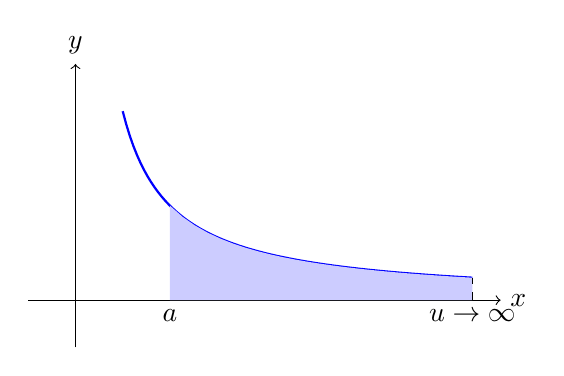
\begin{tikzpicture}[scale=1.2]
    \draw[->] (-0.5,0) -- (4.5,0) node[right] {$x$};
    \draw[->] (0,-0.5) -- (0,2.5) node[above] {$y$};
    \draw[thick, blue, samples=100, domain=0.5:4.2] plot (\x, {1/\x});
    \fill[blue!20, domain=1:4.2] (1,0) -- (1,1) -- plot (\x, {1/\x}) -- (4.2,0) -- cycle;
    \draw[dashed] (4.2,0) -- (4.2, {1/4.2});
    \node[below] at (1,0) {$a$};
    \node[below] at (4.2,0) {$u \to \infty$};
\end{tikzpicture}
\caption{无穷区间积分的示意图}
\end{figure}

类似地，可以定义其他无穷区间上的积分：
\[
\int_{-\infty}^{b}f(x)dx=\lim_{u\to -\infty}\int_u^b f(x)dx,
\]
\[
\int_{-\infty}^{+\infty}f(x)dx=\int_{-\infty}^{c}f(x)dx+\int_c^{+\infty}f(x)dx.
\]
对从 $-\infty$ 到 $+\infty$ 的积分，必须要求两个组成积分\textbf{分别}收敛。分割点 $c$ 的选择不影响收敛性。

\subsubsection{基准：$p$-积分（第一类）}
为了判断复杂函数的收敛性，经常把它们与幂函数 $1/x^p$ 比较。

\begin{theorem}
积分 $\int_1^{+\infty}\frac{1}{x^p}\,dx$：
\begin{itemize}
    \item 当 $p>1$ 时\textbf{收敛}；
    \item 当 $p\le 1$ 时\textbf{发散}。
\end{itemize}
\end{theorem}
\begin{proof}
计算 $\int_1^u x^{-p}\,dx$：
\begin{itemize}
    \item 如果 $p=1$，则 $\ln u\to\infty$，当 $u\to\infty$；
    \item 如果 $p\ne 1$，结果为 $\frac{u^{1-p}-1}{1-p}$。为了收敛，需要 $u^{1-p}\to 0$，这要求 $1-p<0$，即 $p>1$。
\end{itemize}
\end{proof}

\subsection{第二类反常积分（无界函数）}

这类积分出现在有限区间 $[a,b]$ 上，但被积函数 $f(x)$ 在一个或多个点处趋于无穷（有奇点）。

\begin{definition}
如果 $f$ 在 $[a,b)$ 上连续，但在 $b$ 处不连续（例如 $\lim_{x\to b^-}|f(x)|=\infty$），定义
\[
\int_a^b f(x)\,dx=\lim_{\epsilon\to 0^+}\int_a^{b-\epsilon}f(x)\,dx.
\]
\end{definition}

\subsubsection{基准：$p$-积分（第二类）}
注意：奇点情形下的收敛条件与无穷区间情形\textit{相反}。

\begin{theorem}
在区间 $(0,1]$ 上，积分 $\int_0^1\frac{1}{x^p}\,dx$：
\begin{itemize}
    \item 当 $p<1$ 时\textbf{收敛}；
    \item 当 $p\ge 1$ 时\textbf{发散}。
\end{itemize}
\end{theorem}

\subsection{收敛性的一般理论}

在应用实用判别法之前，先建立收敛的严格充要条件。

\subsubsection{Cauchy 准则}
Cauchy 准则很基础，因为它允许在不知道极限值的情况下证明收敛。

\begin{theorem}[反常积分的 Cauchy 准则]
积分 $\int_a^{+\infty}f(x)\,dx$ 收敛，\textbf{当且仅当} 对任意 $\epsilon>0$，存在 $M>a$，使得对所有 $u_2>u_1>M$，都有
\[
\left|\int_{u_1}^{u_2}f(x)\,dx\right|<\epsilon.
\]
\end{theorem}

\subsubsection{绝对收敛与条件收敛}
\begin{itemize}
    \item \textbf{绝对收敛：}$\int |f(x)|\,dx$ 收敛；
    \item \textbf{条件收敛：}$\int f(x)\,dx$ 收敛，但 $\int |f(x)|\,dx$ 发散。
\end{itemize}
\begin{theorem}
如果 $\int_a^{+\infty}|f(x)|\,dx$ 收敛，则 $\int_a^{+\infty}f(x)\,dx$ 收敛。
\end{theorem}

\subsection{收敛判别法}

\subsubsection{直接比较判别法}
\begin{theorem}
设 $f(x)$ 和 $g(x)$ 是 $[a,+\infty)$ 上的连续函数，且对所有 $x\ge a$ 有 $0\le f(x)\le g(x)$。
\begin{enumerate}
    \item 如果 $\int_a^{+\infty}g(x)dx$ 收敛，则 $\int_a^{+\infty}f(x)dx$ 也收敛。
    \item 如果 $\int_a^{+\infty}f(x)dx$ 发散，则 $\int_a^{+\infty}g(x)dx$ 也发散。
\end{enumerate}
\end{theorem}
\textit{直觉：}如果较大曲线下的面积有限，那么较小曲线下的面积也有限；如果较小曲线下的面积无限大，那么较大曲线下的面积必然无限大。

\begin{example}
$\int_1^{+\infty}\frac{\sin^2x}{x^2}dx$ 是否收敛？
\end{example}
\textbf{解：}因为 $0\le \sin^2x\le 1$，所以
\[
0\le \frac{\sin^2x}{x^2}\le \frac{1}{x^2}.
\]
已知 $\int_1^{+\infty}\frac{1}{x^2}dx$ 收敛（$p=2>1$）。由直接比较判别法，$\int_1^{+\infty}\frac{\sin^2x}{x^2}dx$ 收敛。

\subsubsection{极限比较判别法}

有时很难找到直接不等式。极限比较判别法通常更有力。

\begin{theorem}
设 $f(x)$ 和 $g(x)$ 是 $[a,+\infty)$ 上的正连续函数。如果
\[
\lim_{x\to +\infty}\frac{f(x)}{g(x)}=L,
\]
其中 $0<L<+\infty$，则 $\int_a^{+\infty}f(x)dx$ 与 $\int_a^{+\infty}g(x)dx$ 同敛散。
\end{theorem}
如果 $L=0$ 且 $g(x)$ 对应积分收敛，则 $f(x)$ 对应积分收敛；如果 $L=+\infty$ 且 $g(x)$ 对应积分发散，则 $f(x)$ 对应积分发散。

\begin{example}
分析 $\int_1^{+\infty}\frac{x}{1+x^3}dx$。
\end{example}
\textbf{解：}当 $x$ 很大时，常数项 $1$ 可忽略，因此
\[
\frac{x}{1+x^3}\approx \frac{x}{x^3}=\frac{1}{x^2}.
\]
令 $f(x)=\frac{x}{1+x^3}$，$g(x)=\frac{1}{x^2}$。则
\[
\lim_{x\to +\infty}\frac{f(x)}{g(x)}=\lim_{x\to +\infty}\frac{x/(1+x^3)}{1/x^2}=\lim_{x\to +\infty}\frac{x^3}{1+x^3}=1.
\]
由于 $L=1$（有限且为正），并且 $\int_1^{+\infty}\frac{1}{x^2}dx$ 收敛，所以原积分收敛。

对正函数使用比较判别法；对振荡函数，则需要更高级的工具。

\subsubsection{Cauchy 极限比较判别法（阶分析）}
这是判断收敛性最实用的方法。它形式化了把函数与 $1/x^p$ 比较的想法。

\begin{theorem}
设 $f(x)$ 是定义在 $[a,+\infty)$ 上的正函数。考虑 $f(x)$ 乘以测试幂 $x^p$ 后的极限：
\[
\lambda=\lim_{x\to +\infty}x^p f(x).
\]
\begin{enumerate}
    \item \textbf{收敛情形：}如果可以找到 $p>1$，使得 $0\le \lambda<+\infty$，则 $\int_a^{+\infty}f(x)\,dx$ \textbf{收敛}。
    \textit{含义：$f(x)$ 趋于零的速度快于 $1/x$，大致像 $1/x^p$。}
    \item \textbf{发散情形：}如果可以找到 $p\le 1$，使得 $0<\lambda\le +\infty$，则 $\int_a^{+\infty}f(x)\,dx$ \textbf{发散}。
    \textit{含义：$f(x)$ 趋于零的速度慢于或等于 $1/x$。}
\end{enumerate}
\end{theorem}

\begin{example}
检验 $\int_1^{+\infty}\frac{\ln x}{x^2}\,dx$。
由于 $x^2$ 占优，可以猜测收敛。取 $p=1.5$（因为 $1<1.5<2$，留出比较空间）：
\[
\lim_{x\to +\infty}x^{1.5}\frac{\ln x}{x^2}=\lim_{x\to +\infty}\frac{\ln x}{x^{0.5}}=0\quad (\text{由 L'Hôpital 法则}).
\]
因为 $p=1.5>1$ 且极限有限，所以积分收敛。
\end{example}

\subsubsection{Dirichlet 与 Abel 判别法（用于条件收敛）}
这些判别法用于乘积形式的积分 $\int_a^{+\infty}f(x)g(x)\,dx$，通常其中一部分振荡，另一部分衰减。

\begin{theorem}[Dirichlet 判别法]
积分 $\int_a^{+\infty}f(x)g(x)\,dx$ 收敛，如果：
\begin{enumerate}
    \item $f(x)$ 的部分积分有界：存在 $M$，使得对所有 $u>a$，$|\int_a^u f(t)\,dt|\le M$；
    \item $g(x)$ 单调递减，且 $\lim_{x\to +\infty}g(x)=0$。
\end{enumerate}
\end{theorem}
\textit{经典应用：}$\int_0^{+\infty}\frac{\sin x}{x}\,dx$。这里 $f(x)=\sin x$（积分有界），$g(x)=1/x$（单调趋于 $0$）。

\begin{theorem}[Abel 判别法]
积分 $\int_a^{+\infty}f(x)g(x)\,dx$ 收敛，如果：
\begin{enumerate}
    \item $\int_a^{+\infty}f(x)\,dx$ 收敛；
    \item $g(x)$ 单调且有界。
\end{enumerate}
\end{theorem}

\subsubsection{Cauchy 主值（P.V.）}

在某些发散积分中，如果以对称方式取极限，正负面积可能相互抵消。这个值称为 Cauchy 主值。

\begin{definition}
\begin{enumerate}
    \item 对 $c\in(a,b)$ 处的奇点：
    \[
    \text{P.V.}\int_a^b f(x)\,dx=\lim_{\epsilon\to 0^+}\left(\int_a^{c-\epsilon}f(x)\,dx+\int_{c+\epsilon}^{b}f(x)\,dx\right).
    \]
    \item 对无穷区间 $(-\infty,+\infty)$：
    \[
    \text{P.V.}\int_{-\infty}^{+\infty}f(x)\,dx=\lim_{R\to +\infty}\int_{-R}^{R}f(x)\,dx.
    \]
\end{enumerate}
\end{definition}

\begin{remark}
\textbf{收敛 $\implies$ 主值存在}，但反过来不成立。
\end{remark}

\begin{example}
考虑 $f(x)=\frac{1}{x}$ 在 $[-1,1]$ 上的积分。
\begin{itemize}
    \item \textbf{反常积分：}
    \[
    \int_{-1}^{1}\frac{1}{x}\,dx=\int_{-1}^{0}\frac{1}{x}\,dx+\int_0^1\frac{1}{x}\,dx.
    \]
    由于 $\int_{\epsilon}^{1}\frac{1}{x}\,dx=-\ln\epsilon\to\infty$，标准反常积分\textbf{发散}。
    \item \textbf{主值：}
    \[
    \text{P.V.}\int_{-1}^{1}\frac{1}{x}\,dx=\lim_{\epsilon\to 0^+}\left(\int_{-1}^{-\epsilon}\frac{1}{x}\,dx+\int_{\epsilon}^{1}\frac{1}{x}\,dx\right)=0.
    \]
    这是由函数的奇对称性造成的。
\end{itemize}
\end{example}

\subsubsection{综合例子：Gamma 函数}
\[
\Gamma(s)=\int_0^{+\infty}x^{s-1}e^{-x}\,dx.
\]
这个积分需要同时分析零点附近的奇性和无穷远处的行为。
\begin{itemize}
    \item \textbf{在 $0$ 附近：}如果 $s<1$，$x^{s-1}$ 有奇性。由于 $e^{-x}\approx 1$，它的行为类似于 $\int_0^1\frac{1}{x^{1-s}}dx$。由第二类 $p$-积分判别法，它在 $1-s<1$，即 $s>0$ 时收敛。
    \item \textbf{在 $+\infty$ 处：}$e^{-x}$ 的衰减快于任意幂 $x^p$ 的增长。用 $1/x^2$ 作极限比较：
    \[
    \lim_{x\to\infty}x^2(x^{s-1}e^{-x})=0.
    \]
    因而在无穷远处对所有 $s$ 都收敛。
\end{itemize}
\textbf{结论：}该积分在 $s>0$ 时收敛。

在本章最后，用所学知识解决一个有趣问题：Gabriel 号角。

考虑有一个号角，其横截面是圆，而纵截面由函数 $y=\frac{1}{x}$，$x\in(1,\infty)$ 描述。

先计算号角的体积：
\[
V=\pi\int_1^{+\infty}\left(\frac{1}{x}\right)^2dx=\pi\left[-\frac{1}{x}\right]_1^{+\infty}=\pi.
\]
可以看到，这个号角有有限体积。

再计算其表面积：
\[
S=2\pi\int_1^{+\infty}\frac{1}{x}\sqrt{1+\frac{1}{x^4}}dx\ge 2\pi\int_1^{+\infty}\frac{1}{x}dx=+\infty.
\]
表面积对应的积分发散。

这里出现了一个非常有趣的悖论：可以用有限多的油漆填满这个号角，但这桶油漆却无法涂满号角的内壁。

这个结果与我们的朴素理解相矛盾。

本章结束时要记住：这不是终点，而是一道入口。数学分析的旅程还会继续。在\textbf{第 4 章}中，我们会把这些基础扩展到更高维，进一步研究曲线和曲面，并遇到更多优美而出人意料的结果。这个来自无穷领域的号角之声，邀请我们继续探索。

在后续章节中，我们还会进入更多分析学高级主题，例如多变量微积分、微分方程、复分析和泛函分析。每一个领域都建立在本章发展的概念之上，并各自带来独特的洞见与挑战。希望读者带着本章获得的严谨工具和深入理解，继续探索下去。

\vspace{1cm}
\noindent
\textbf{参考文献：} \\
Mathematical Analysis (Third Edition), Chen, J., Higher Education Press \\
The Real Numbers and Real Analysis, Ethan D. Bloch, Springer

\cleardoublepage


\chapter{线性代数}
\begin{quote}
\emph{
在完成分析部分的第一阶段之后，我们现在进入一个新的章节：线性代数。它是数学中一个相当不同的部分。
}

\emph{
不同于分析学和微积分，线性代数更强调几何理解。证明依然重要，但对学习者来说，更关键的是建立关于这一学科的几何直觉。这里需要说明的是，直觉不同于想象。虽然我们只能直接想象三维欧几里得空间，但直觉可以把我们带向更高维的空间，也可以带向更抽象的线性空间。
}

\emph{
在这一部分中，我们会从解线性方程组开始，然后研究一种特殊的线性空间：向量空间。最后，我们会进入更加抽象的部分：线性空间。它为我们提供一种新的工具，用来研究更一般形式的代数结构和系统。
}

\emph{
更具体地说，在最后关于抽象线性空间的部分中，我们会讨论线性无关、基、维数和线性变换等关键概念。理解这些基础概念，可以帮助我们把看起来彼此不同的数学对象，例如函数、多项式和矩阵，统一到同一个强有力的框架之下。这种抽象并不只是学术上的训练；它也为处理微分方程、数据科学、量子力学和工程优化等领域中的复杂问题提供了基本语言和工具。在研究 $\mathbb{R}^n$ 时建立起来的几何直觉，会在我们进入这些高维且抽象的领域时发挥不可替代的作用。也正因为如此，线性代数成为现代数学中最基础、应用最广泛的领域之一。
}

\emph{
在后面的章节中，我们还会介绍代数学的另一分支，即抽象代数。线性代数更关注多元方程，而抽象代数则研究高次方程的解结构，这是数学中更加抽象的一部分。不过，即使在抽象代数中，我们仍然需要线性代数的知识。因此，现在就让我们开始吧。
}
\end{quote}

\section{线性方程与矩阵}

\subsection{线性方程组}

我相信大多数读者都见过如下形式的方程组：

\[
\begin{cases}
x+y=1\\
x-y =0
\end{cases}
\]

它们可能有不同数量的变量和方程，但它们共享一个共同特征：\textbf{每一个方程都是线性的。}变量只以一次幂出现，变量之间没有乘积，例如 $xy$，也没有非线性函数，例如 $\sin(x)$ 或 $\sqrt{x}$。

对于这种方程系统，我们称其为\textbf{线性方程组}。它的一般形式包含 $m$ 个方程和 $n$ 个变量，也称为一个 $m \times n$ 系统：

\[
\begin{cases}
a_{11}x_1 + a_{12}x_2 + \cdots + a_{1n}x_n = b_1\\
a_{21}x_1 + a_{22}x_2 + \cdots + a_{2n}x_n = b_2\\
\quad \vdots \\
a_{m1}x_1 + a_{m2}x_2 + \cdots + a_{mn}x_n = b_m
\end{cases}
\]
其中，$x_1,\ldots,x_n$ 是\textbf{变量}，也就是未知量；$a_{ij}$ 是\textbf{系数}；$b_1,\ldots,b_m$ 是\textbf{常数项}。

方程组的一个\textbf{解}，是指一组数 $(s_1,s_2,\ldots,s_n)$，当它们分别代入 $(x_1,x_2,\ldots,x_n)$ 时，能够同时满足全部 $m$ 个方程。所有可能解构成的集合称为\textbf{解集}。

\begin{example}[一个 $2\times 2$ 系统]
考虑方程组
\[
\begin{cases}
x_1 + x_2 = 3 \\
x_1 - x_2 = -1
\end{cases}
\]
我们可以用初等代数求解。
\begin{enumerate}
    \item \textbf{代入法：}由第一个方程得到 $x_2 = 3-x_1$。把它代入第二个方程，得到 $x_1-(3-x_1)=-1$，即 $2x_1-3=-1$，所以 $2x_1=2$，从而 $x_1=1$。于是 $x_2=3-1=2$。唯一解是 $(1,2)$。
    \item \textbf{消元法：}将两个方程相加：$(x_1+x_2)+(x_1-x_2)=3+(-1)$，得到 $2x_1=2$，所以 $x_1=1$。用第一个方程减去第二个方程：$(x_1+x_2)-(x_1-x_2)=3-(-1)$，得到 $2x_2=4$，所以 $x_2=2$。
\end{enumerate}
因此解集只包含一个点 $(1,2)$。
\end{example}

在线性代数中，我们关心三个问题：
\begin{enumerate}
    \item \textbf{存在性：}解是否存在？也就是说，系统是否\textbf{相容}？
    \item \textbf{唯一性：}如果解存在，它是否唯一？
    \item \textbf{计算性：}如果解存在，应该怎样求出它们？
\end{enumerate}

从几何角度看，对于一个 $2\times 2$ 系统，每一个方程都表示 $\mathbb{R}^2$ 平面中的一条直线。解集就是这些直线的交集。
\begin{itemize}
    \item \textbf{唯一解：}两条直线交于一个点。
    \item \textbf{无解：}两条直线平行且不重合。
    \item \textbf{无穷多解：}两个方程表示同一条直线。
\end{itemize}

对于一个 $3\times 3$ 系统，每一个方程都是 $\mathbb{R}^3$ 中的一个平面。三个平面的交集可能是一个点、一条直线、一个平面，也可能为空集。

当方程规模变大时，例如 $5$ 个方程、$5$ 个变量，代入法和消元法会变得非常繁琐。因此，我们需要一种更系统、更高效的方法。矩阵正是在这里登场的。

\subsection{矩阵代数}

\subsubsection{矩阵记号与特殊矩阵}

新方法的本质，是在不改变解集的情况下操作方程。我们注意到，方程组中的全部信息都包含在系数 $a_{ij}$ 和常数项 $b_i$ 之中。变量名 $x_1,x_2,\ldots$ 只是占位符。因此，我们可以把整个系统编码进一个紧凑的矩形数组中，这个数组称为\textbf{矩阵}。

\begin{definition}
\textbf{矩阵}是由数字组成的矩形数组，这些数字称为矩阵的\textbf{元素}或\textbf{项}。一个具有 $m$ 行和 $n$ 列的矩阵称为 $m\times n$ 矩阵。
\end{definition}

对于一般线性方程组，我们定义两个重要矩阵。

\textbf{系数矩阵}为
\[ \textbf{A} = \begin{pmatrix}
a_{11} & a_{12} & \cdots & a_{1n} \\
a_{21} & a_{22} & \cdots & a_{2n} \\
\vdots & \vdots & \ddots & \vdots \\
a_{m1} & a_{m2} & \cdots & a_{mn}
\end{pmatrix} \]
我们也可以把它记作 $A=[a_{ij}]$。其中 $a_{ij}$ 表示第 $i$ 行第 $j$ 列的元素。

包含常数项的矩阵称为\textbf{增广矩阵}：
\[ (A \mid \mathbf{b}) = \left(\begin{array}{cccc|c}
a_{11} & a_{12} & \cdots & a_{1n} & b_1 \\
a_{21} & a_{22} & \cdots & a_{2n} & b_2 \\
\vdots & \vdots & \ddots & \vdots & \vdots \\
a_{m1} & a_{m2} & \cdots & a_{mn} & b_m
\end{array}\right) \]
因此，求解方程组就等价于操作这个增广矩阵。

\newpage

\begin{example}
方程组
\[
\begin{cases}
x_1 - 2x_2 + x_3 = 0 \\
2x_2 - 8x_3 = 8 \\
5x_1 - 5x_3 = 10
\end{cases}
\]
的系数矩阵为
\[ A = \begin{pmatrix} 1 & -2 & 1 \\ 0 & 2 & -8 \\ 5 & 0 & -5 \end{pmatrix} \]
增广矩阵为
\[ (A \mid \mathbf{b}) = \left(\begin{array}{ccc|c} 1 & -2 & 1 & 0 \\ 0 & 2 & -8 & 8 \\ 5 & 0 & -5 & 10 \end{array}\right) \]
\end{example}

\paragraph{矩阵术语与特殊矩阵}

\begin{itemize}
    \item \textbf{大小/维度：}一个有 $m$ 行和 $n$ 列的矩阵 $A$ 的大小为 $m\times n$。
    \item \textbf{方阵：}如果矩阵的行数等于列数，即 $m=n$，则称该矩阵为\textbf{方阵}。
    \item \textbf{相等：}两个矩阵 $A=[a_{ij}]$ 和 $B=[b_{ij}]$ \textbf{相等}，当且仅当它们大小相同，并且每一个对应元素都相等，即对所有 $i,j$ 都有 $a_{ij}=b_{ij}$。
    \item \textbf{主对角线：}在方阵中，元素 $a_{11},a_{22},\ldots,a_{nn}$ 构成\textbf{主对角线}。
    \item \textbf{副对角线：}在方阵中，从右上角到左下角的对角线
    $$a_{1n}, a_{2,n-1}, \ldots, a_{n1}$$
    称为\textbf{副对角线}。
\end{itemize}

下面列出几类特殊矩阵：

\begin{enumerate}
    \item \textbf{零矩阵：}所有元素都为 $0$ 的矩阵，大小可以任意。通常记为 $\mathbf{0}$ 或 $\mathbf{0}_{m\times n}$。
    \[ \mathbf{0} = \begin{pmatrix} 0 & 0 & \cdots & 0 \\ \vdots & \vdots & \ddots & \vdots \\ 0 & 0 & \cdots & 0 \end{pmatrix} \]
    \item \textbf{单位矩阵：}方阵 $I_n$，或简记为 $I$，其主对角线元素全为 $1$，其他元素全为 $0$。
    \[ I_3 = \begin{pmatrix} 1 & 0 & 0 \\ 0 & 1 & 0 \\ 0 & 0 & 1 \end{pmatrix} \]
    单位矩阵是乘法单位元：在维度相容时，$AI=A$ 且 $IA=A$。
    \item \textbf{对角矩阵：}主对角线之外的所有元素都为 $0$ 的方阵。
    \[ D = \begin{pmatrix} 3 & 0 & 0 \\ 0 & -1 & 0 \\ 0 & 0 & 5 \end{pmatrix} \]
    \item \textbf{上三角矩阵：}主对角线下方元素全为 $0$ 的方阵，即当 $i>j$ 时 $a_{ij}=0$。
    \[ U = \begin{pmatrix} 1 & 4 & -1 \\ 0 & 2 & 7 \\ 0 & 0 & 3 \end{pmatrix} \]
    \item \textbf{下三角矩阵：}主对角线上方元素全为 $0$ 的方阵，即当 $i<j$ 时 $a_{ij}=0$。
    \[ L = \begin{pmatrix} 1 & 0 & 0 \\ 5 & 2 & 0 \\ -1 & 0 & 3 \end{pmatrix} \]
    \item \textbf{转置：}一个 $m\times n$ 矩阵 $A$ 的\textbf{转置}记作 $A^T$，或 $A'$，它是通过交换矩阵的行和列得到的 $n\times m$ 矩阵。也就是说，$(A^T)_{ij}=A_{ji}$。
    \[ A = \begin{pmatrix} 1 & 2 & 3 \\ 4 & 5 & 6 \end{pmatrix} \quad \implies \quad A^T = \begin{pmatrix} 1 & 4 \\ 2 & 5 \\ 3 & 6 \end{pmatrix} \]
    \item \textbf{对称矩阵：}若方阵 $A$ 满足 $A^T=A$，则称其为对称矩阵。这意味着对所有 $i,j$，都有 $a_{ij}=a_{ji}$。
    \[ S = \begin{pmatrix} 1 & 5 & -1 \\ 5 & 2 & 0 \\ -1 & 0 & 3 \end{pmatrix} \]
    \item \textbf{反对称矩阵：}若方阵 $A$ 满足 $A^T=-A$，则称其为反对称矩阵。这意味着 $a_{ij}=-a_{ji}$，并且 $a_{ii}=0$。
    \[ K = \begin{pmatrix} 0 & 5 & -1 \\ -5 & 0 & 2 \\ 1 & -2 & 0 \end{pmatrix} \]
\end{enumerate}

\subsubsection{矩阵运算}

我们可以在矩阵上定义代数运算。

\paragraph{矩阵加法与数乘}
\begin{definition}
设 $A=[a_{ij}]$ 和 $B=[b_{ij}]$ 是两个\textbf{大小相同}的 $m\times n$ 矩阵。
\begin{enumerate}
    \item \textbf{加法：}它们的和 $A+B$ 是 $m\times n$ 矩阵 $C=[c_{ij}]$，其中 $c_{ij}=a_{ij}+b_{ij}$。
    \item \textbf{数乘：}设 $c$ 是一个标量，也就是一个实数。矩阵 $cA$ 是 $m\times n$ 矩阵 $D=[d_{ij}]$，其中 $d_{ij}=c\cdot a_{ij}$。
\end{enumerate}
矩阵减法定义为 $A-B=A+(-1)B$。
\end{definition}

\begin{example}
设 $A=\begin{pmatrix}1&2\\3&4\end{pmatrix}$，$B=\begin{pmatrix}5&0\\-1&7\end{pmatrix}$。则
\[ A+B = \begin{pmatrix} 1+5 & 2+0 \\ 3-1 & 4+7 \end{pmatrix} = \begin{pmatrix} 6 & 2 \\ 2 & 11 \end{pmatrix} \]
\[ 3A = \begin{pmatrix} 3(1) & 3(2) \\ 3(3) & 3(4) \end{pmatrix} = \begin{pmatrix} 3 & 6 \\ 9 & 12 \end{pmatrix} \]
注意，$A + \begin{pmatrix}1&2&3\\4&5&6\end{pmatrix}$ 是\textbf{没有定义的}，因为矩阵大小不匹配。
\end{example}

这些运算满足熟悉的性质：
\begin{property}[加法与数乘的性质]
设 $A,B,C$ 是 $m\times n$ 矩阵，$c,d$ 是标量。
\begin{enumerate}
    \item $A+B=B+A$，即加法交换律。
    \item $(A+B)+C=A+(B+C)$，即加法结合律。
    \item $A+\mathbf{0}=A$，即加法单位元。
    \item $A+(-A)=\mathbf{0}$，即加法逆元。
    \item $c(A+B)=cA+cB$，即分配律。
    \item $(c+d)A=cA+dA$，即分配律。
    \item $c(dA)=(cd)A$。
    \item $1A=A$。
\end{enumerate}
\end{property}
\begin{remark}
这八条性质再加上封闭性，恰好就是\textbf{向量空间}的公理。所有 $m\times n$ 矩阵构成的集合 $M_{m\times n}$ 是向量空间的一个典型例子。
\end{remark}

\newpage

\paragraph{矩阵乘法}
矩阵乘法更复杂，也更加重要。

\begin{definition}[矩阵乘法]
设 $A$ 是一个 $m\times \mathbf{n}$ 矩阵，$B$ 是一个 $\mathbf{n}\times p$ 矩阵。它们的\textbf{乘积} $AB$ 是一个 $m\times p$ 矩阵 $C=[c_{ij}]$。
$AB$ 中第 $i$ 行第 $j$ 列的元素 $c_{ij}$，由 $A$ 的第 $i$ 行与 $B$ 的第 $j$ 列作\textbf{点积}得到：
\[ c_{ij} = (A\text{ 的第 }i\text{ 行})\cdot (B\text{ 的第 }j\text{ 列}) = a_{i1}b_{1j}+a_{i2}b_{2j}+\cdots+a_{in}b_{nj} \]
\[ c_{ij}=\sum_{k=1}^{n} a_{ik}b_{kj} \]
\end{definition}

\textbf{关键注意：}乘积 $AB$ 只有在 \textbf{$A$ 的列数}等于\textbf{$B$ 的行数}时才有定义。
\[
(m\times \mathbf{n})\cdot(\mathbf{n}\times p)\to(m\times p)
\]

\begin{example}
设 $A=\begin{pmatrix}1&2&3\\4&5&6\end{pmatrix}$，它是 $2\times3$ 矩阵；$B=\begin{pmatrix}7&8\\9&0\\1&2\end{pmatrix}$，它是 $3\times2$ 矩阵。乘积 $AB$ 是一个 $2\times2$ 矩阵。
\[
AB = \begin{pmatrix}
(1\cdot 7 + 2\cdot 9 + 3\cdot 1) & (1\cdot 8 + 2\cdot 0 + 3\cdot 2) \\
(4\cdot 7 + 5\cdot 9 + 6\cdot 1) & (4\cdot 8 + 5\cdot 0 + 6\cdot 2)
\end{pmatrix}
= \begin{pmatrix} 28 & 14 \\ 79 & 44 \end{pmatrix}
\]
再计算 $BA$。它会是一个 $3\times3$ 矩阵。
\[
BA = \begin{pmatrix} 7 & 8 \\ 9 & 0 \\ 1 & 2 \end{pmatrix} \begin{pmatrix} 1 & 2 & 3 \\ 4 & 5 & 6 \end{pmatrix}
= \begin{pmatrix}
39 & 54 & 69 \\
9 & 18 & 27 \\
9 & 12 & 15
\end{pmatrix}
\]
\end{example}

\begin{property}[矩阵乘法的性质]
设 $A,B,C$ 是维度相容的矩阵，$c$ 是标量。
\begin{enumerate}
    \item \textbf{警告：}一般来说 $AB\neq BA$。矩阵乘法\textbf{不满足交换律}。
    \item $A(BC)=(AB)C$，即结合律。
    \item $A(B+C)=AB+AC$，即左分配律。
    \item $(A+B)C=AC+BC$，即右分配律。
    \item $c(AB)=(cA)B=A(cB)$。
    \item $I_mA=A=AI_n$，即乘法单位元。
\end{enumerate}
\end{property}

虽然一般矩阵并不满足 $AB=BA$，但我们仍然希望找到一些具有这种性质的矩阵。后续章节中会介绍一些特殊矩阵，它们可以满足这种交换关系。

上面这些性质的证明留给读者完成。

\begin{remark}
请记住，$\textbf{A}\textbf{b}=\textbf{0}$ 不能推出 $A=0$ 或 $B=0$。这也是矩阵运算中反直觉现象的一个例子。
\end{remark}

\begin{definition}
设 $A$ 是一个 $n$ 阶方阵，$m\in\mathbb{N}^{*}$。$m$ 个 $A$ 的乘积称为 $A$ 的 $m$ 次幂，记作 $A^m$。特别地，我们定义 $A^0=I_n$。
\end{definition}

矩阵幂的计算\textbf{基本上}遵循通常的代数规则，但要注意乘法顺序。例如：
\[(A+B)^2 = A^2 + AB + BA + B^2\]
\[(A+B)(A-B) = A^2 - AB + BA - B^2\]

\begin{definition}
设 $A=(a_{ij})_{m\times n}$。若 $A^T=(b_{kl})_{n\times m}$ 满足 $b_{kl}=a_{lk}$，其中 $k=1,2,\cdots,n$，$l=1,2,\cdots,m$，则称 $A^T$ 为 $A$ 的转置矩阵。
\end{definition}

\begin{property}[转置的性质]
\begin{enumerate}
    \item $(A^T)^T=A$。
    \item $(A+B)^T=A^T+B^T$。
    \item $(cA)^T=cA^T$。
    \item \textbf{反序性质：}$(AB)^T=B^TA^T$。
    \item $(A^m)^T=(A^T)^m$。
\end{enumerate}
\end{property}
\begin{proof}[证明 $(AB)^T=B^TA^T$]
设 $A$ 是 $m\times n$ 矩阵，$B$ 是 $n\times p$ 矩阵。则 $AB$ 是 $m\times p$ 矩阵，因此 $(AB)^T$ 是 $p\times m$ 矩阵。
同时，$B^T$ 是 $p\times n$ 矩阵，$A^T$ 是 $n\times m$ 矩阵，所以 $B^TA^T$ 也是 $p\times m$ 矩阵。两者大小相同。
令 $C=AB$。$C^T$ 的第 $(i,j)$ 个元素是 $C_{ji}$。
根据定义，
\[
C_{ji}=\sum_{k=1}^{n}A_{jk}B_{ki}.
\]
再令 $D=B^TA^T$。$D$ 的第 $(i,j)$ 个元素为
\[ D_{ij}=\sum_{k=1}^{n}(B^T)_{ik}(A^T)_{kj}. \]
由转置定义，$(B^T)_{ik}=B_{ki}$，$(A^T)_{kj}=A_{jk}$。
因此
\[
D_{ij}=\sum_{k=1}^{n}B_{ki}A_{jk}=\sum_{k=1}^{n}A_{jk}B_{ki}.
\]
所以 $D_{ij}=C_{ji}=(C^T)_{ij}$。由于所有元素都相等，得到 $B^TA^T=(AB)^T$。
\end{proof}

方阵还有一个重要数值，后面会用到。

\begin{definition}[矩阵的迹]
设 $A=(a_{ij})$ 是一个 $n$ 阶方阵。数
\[
\sum_{i=1}^{n}a_{ii}
\]
称为矩阵 $A$ 的迹，记作 $\operatorname{tr}(A)$。
\end{definition}

\begin{property}
\begin{enumerate}
    \item $\operatorname{tr}(A+B)=\operatorname{tr}(A)+\operatorname{tr}(B)$。
    \item $\operatorname{tr}(kA)=k\operatorname{tr}(A)$。
    \item $\operatorname{tr}(AB)=\operatorname{tr}(BA)$。
    \item $\operatorname{tr}(A^T)=\operatorname{tr}(A)$。
\end{enumerate}
\end{property}

\subsubsection*{分块矩阵的定义}
分块矩阵是指把一个矩阵划分成若干较小的子矩阵，这些子矩阵称为\textbf{块}。这种划分可以通过水平线和竖直线把矩阵分割成矩形块来实现。分块之后，我们可以把一个大矩阵看成由若干更小、更易处理的部分组成。

若 $A$ 是一个 $m\times n$ 矩阵，可以如下分块：
\[
A = \begin{bmatrix}
    A_{11} & A_{12} & \cdots & A_{1q} \\
    A_{21} & A_{22} & \cdots & A_{2q} \\
    \vdots & \vdots & \ddots & \vdots \\
    A_{p1} & A_{p2} & \cdots & A_{pq}
\end{bmatrix}
\]
其中，每个 $A_{ij}$ 都是 $A$ 的一个子矩阵，也就是一个块。块的大小必须相容：例如同一列块中的子矩阵列数要一致，同一行块中的子矩阵行数也要一致。

\textbf{分块矩阵的运算}

\paragraph*{分块矩阵加法}
如果两个矩阵 $A$ 与 $B$ 被分成对应块大小\textbf{相同}的分块形式，则可以按块相加：
\[
A+B=\begin{bmatrix}
A_{11}+B_{11} & A_{12}+B_{12} & \cdots\\
A_{21}+B_{21} & A_{22}+B_{22} & \cdots\\
\vdots & \vdots & \ddots
\end{bmatrix}
\]
为了使加法有定义，每一对对应块 $A_{ij}$ 和 $B_{ij}$ 必须大小相同。

\paragraph*{分块矩阵数乘}
数乘通过把每一个块都乘以该标量来完成：
\[
cA=\begin{bmatrix}
cA_{11} & cA_{12} & \cdots\\
cA_{21} & cA_{22} & \cdots\\
\vdots & \vdots & \ddots
\end{bmatrix}
\]

\paragraph*{分块矩阵乘法}
如果 $A$ 是一个 $m\times n$ 的分块矩阵，$B$ 是一个 $n\times p$ 的分块矩阵，并且 $A$ 的列块数等于 $B$ 的行块数，那么乘积 $C=AB$ 可以按块计算：
\[
C_{ij}=\sum_{k=1}^{q}A_{ik}B_{kj}.
\]
这要求每一个 $A_{ik}$ 的列数都等于相应 $B_{kj}$ 的行数。所得的块 $C_{ij}$ 是对应块乘积之和。

\textbf{例：}若 $A=\begin{bmatrix}A_{11}&A_{12}\\A_{21}&A_{22}\end{bmatrix}$，$B=\begin{bmatrix}B_{11}\\B_{21}\end{bmatrix}$，则
\[
AB=\begin{bmatrix}
A_{11}B_{11}+A_{12}B_{21}\\
A_{21}B_{11}+A_{22}B_{21}
\end{bmatrix}.
\]

\paragraph*{分块矩阵转置}
分块矩阵的转置，是先把每个块转置，再把块的位置也转置：
\[
A^\top=\begin{bmatrix}
A_{11}^\top & A_{21}^\top & \cdots\\
A_{12}^\top & A_{22}^\top & \cdots\\
\vdots & \vdots & \ddots
\end{bmatrix}
\]
注意，块的位置也会发生转置，例如原来位于 $(1,2)$ 的块，转置后会出现在 $(2,1)$ 的位置。

\paragraph*{分块对角矩阵}
分块对角矩阵是指非对角块全为零矩阵的方形分块矩阵：
\[
A=\begin{bmatrix}
A_{11}&0&\cdots&0\\
0&A_{22}&\cdots&0\\
\vdots&\vdots&\ddots&\vdots\\
0&0&\cdots&A_{pp}
\end{bmatrix}
\]
分块对角矩阵的运算会简化，因为不同对角块可以独立处理。例如，如果各对角块都可逆，则分块对角矩阵的逆就是由这些对角块的逆组成的分块对角矩阵。

\subsubsection*{使用分块矩阵的优势}
\begin{itemize}
    \item 可以把大矩阵拆成较小部分，从而简化运算。
    \item 有利于并行计算。
    \item 在理论证明中，可以通过分块结构进行归纳。
    \item 在数值线性代数中，分块矩阵常用于构造高效算法。
\end{itemize}

\begin{definition}
一个 $n\times n$ 方阵 $A$ 称为\textbf{可逆}，或称为\textbf{非奇异}，如果存在一个 $n\times n$ 矩阵 $B$，使得
\[ AB=I_n \quad \text{且}\quad BA=I_n. \]
这个矩阵 $B$ 是唯一的，称为 $A$ 的\textbf{逆矩阵}，记作 $A^{-1}$。如果这样的矩阵 $B$ 不存在，则称 $A$ 为\textbf{奇异矩阵}，也就是\textbf{不可逆矩阵}。
\end{definition}

\begin{example}[$2\times2$ 矩阵的逆]
设 $A=\begin{pmatrix}a&b\\c&d\end{pmatrix}$。如果 $ad-bc\neq0$，则 $A$ 可逆，并且
\[ A^{-1}=\frac{1}{ad-bc}\begin{pmatrix}d&-b\\-c&a\end{pmatrix}. \]
如果 $ad-bc=0$，则 $A$ 奇异。数 $ad-bc$ 称为 $A$ 的\textbf{行列式}。
\end{example}

\begin{property}[逆矩阵的性质]
设 $A$ 和 $B$ 是可逆的 $n\times n$ 矩阵。
\begin{enumerate}
    \item $(A^{-1})^{-1}=A$。
    \item $(AB)^{-1}=B^{-1}A^{-1}$，注意顺序反过来了。
    \item $(A^T)^{-1}=(A^{-1})^T$。
    \item 当 $c\neq0$ 时，$(cA)^{-1}=\frac{1}{c}A^{-1}$。
\end{enumerate}
\end{property}
\begin{proof}[证明 $(AB)^{-1}=B^{-1}A^{-1}$]
只需要检查定义：
\[ (AB)(B^{-1}A^{-1})=A(BB^{-1})A^{-1}=AIA^{-1}=AA^{-1}=I. \]
\[ (B^{-1}A^{-1})(AB)=B^{-1}(A^{-1}A)B=B^{-1}IB=B^{-1}B=I. \]
因此 $B^{-1}A^{-1}$ 满足逆矩阵的定义，它必然是 $AB$ 的逆。
\end{proof}

\subsection{线性方程组的求解}

现在回到主问题：求解 $m$ 个方程、$n$ 个变量的线性方程组。总体思想就是\textbf{高斯消元法}：把增广矩阵变换成更简单的形式，然后直接读出解。

\subsubsection{初等行变换}

我们可以对增广矩阵进行操作，这些操作对应于对原方程的操作，并且\textbf{不会改变解集}。

\begin{definition}
三类\textbf{初等行变换}为：
\begin{enumerate}
    \item \textbf{替换：}把某一行加上另一行的若干倍，记作 $R_i\to R_i+cR_j$。
    \item \textbf{交换：}交换两行，记作 $R_i\leftrightarrow R_j$。
    \item \textbf{倍乘：}把某一行的所有元素都乘以一个非零常数，记作 $R_i\to cR_i$，其中 $c\neq0$。
\end{enumerate}
\end{definition}

\begin{definition}
如果矩阵 $B$ 可以由矩阵 $A$ 经过一系列初等行变换得到，则称 $A$ 与 $B$ \textbf{行等价}，记作 $A\sim B$。
\end{definition}

\begin{theorem}
如果两个线性方程组的增广矩阵行等价，那么这两个方程组具有\textbf{相同的解集}。
\end{theorem}
\begin{proof}[说明]
\begin{itemize}
    \item 替换 $R_i\to R_i+cR_j$ 对应于把第 $j$ 个方程的 $c$ 倍加到第 $i$ 个方程上。这个步骤可逆，反向操作为 $R_i\to R_i-cR_j$。原系统的任意解仍是新系统的解，反过来也一样。
    \item 交换 $R_i\leftrightarrow R_j$ 只是交换两个方程的顺序，显然不影响解集。
    \item 倍乘 $R_i\to cR_i$，其中 $c\neq0$，对应于把一个方程乘以 $c$。它也可逆，反向操作是乘以 $1/c$，所以不改变解集。
\end{itemize}
\end{proof}

\subsubsection{行阶梯形与秩}

目标是用初等行变换把矩阵化成一种“阶梯状”的简单形式。

\begin{definition}
如果一个矩阵满足下面条件，则称它处于\textbf{行阶梯形}，记作 REF：
\begin{enumerate}
    \item 所有非零行都在全零行的上方。
    \item 每一行的\textbf{首项}，也称为\textbf{主元}，即该行最左边的非零元素，位于上一行首项的右侧。
    \item 每个首项所在列中，位于首项下方的元素全为零。
\end{enumerate}
\end{definition}

\begin{definition}
如果一个矩阵处于 REF，并且还满足下面条件，则称它处于\textbf{简化行阶梯形}，记作 RREF：
\begin{enumerate}
    \item 每个非零行的首项都是 $1$。
    \item 每个首 $1$ 是其所在列中唯一的非零元素。
\end{enumerate}
\end{definition}

\begin{example}
\textbf{REF}：
\[ \begin{pmatrix} \fbox{2} & 3 & 4 & 5 \\ 0 & \fbox{1} & 6 & 7 \\ 0 & 0 & 0 & \fbox{8} \\ 0 & 0 & 0 & 0 \end{pmatrix} \]
\textbf{RREF}：
\[ \begin{pmatrix} \fbox{1} & 0 & -1 & 0 \\ 0 & \fbox{1} & 2 & 0 \\ 0 & 0 & 0 & \fbox{1} \\ 0 & 0 & 0 & 0 \end{pmatrix} \]
方框中的元素是主元。
\end{example}

\begin{theorem}
每一个矩阵都行等价于唯一的\textbf{简化行阶梯形}。
\end{theorem}

把矩阵化为 REF 或 RREF 的算法，是我们求解线性方程组的核心方法。

\begin{definition}
\begin{itemize}
    \item \textbf{高斯消元法}是指使用初等行变换把矩阵化为 REF 的过程。
    \item \textbf{高斯--若尔当消元法}是指使用初等行变换把矩阵化为 RREF 的过程。
\end{itemize}
\end{definition}

\paragraph{算法：高斯--若尔当消元法}
我们完整求解一个方程组：
\[
\begin{cases}
x_2+3x_3=4\\
x_1+x_2+x_3=1\\
2x_1+3x_2+4x_3=7
\end{cases}
\]
增广矩阵为
\[
\left(\begin{array}{ccc|c}
0 & 1 & 3 & 4 \\
1 & 1 & 1 & 1 \\
2 & 3 & 4 & 7
\end{array}\right).
\]
\textbf{第一步：前向阶段，化为 REF。}
我们需要在左上角 $(1,1)$ 位置放置主元，因此先与第二行交换：
\[
\left(\begin{array}{ccc|c}
1 & 1 & 1 & 1 \\
0 & 1 & 3 & 4 \\
2 & 3 & 4 & 7
\end{array}\right) \quad (R_1\leftrightarrow R_2).
\]
消去第一个主元下方的元素：
\[
\left(\begin{array}{ccc|c}
1 & 1 & 1 & 1 \\
0 & 1 & 3 & 4 \\
0 & 1 & 2 & 5
\end{array}\right) \quad (R_3\to R_3-2R_1).
\]
然后处理第二个主元 $(2,2)$。它已经是 $1$，继续消去它下方的元素：
\[
\left(\begin{array}{ccc|c}
1 & 1 & 1 & 1 \\
0 & 1 & 3 & 4 \\
0 & 0 & -1 & 1
\end{array}\right) \quad (R_3\to R_3-R_2).
\]
此时矩阵已经处于\textbf{行阶梯形}，高斯消元完成。
如果在这里停下，可以使用\textbf{回代法}：
由 $R_3$ 得 $-x_3=1$，所以 $x_3=-1$。
由 $R_2$ 得 $x_2+3x_3=4$，因此 $x_2+3(-1)=4$，所以 $x_2=7$。
由 $R_1$ 得 $x_1+x_2+x_3=1$，因此 $x_1+7+(-1)=1$，所以 $x_1=-5$。
唯一解为 $(-5,7,-1)$。

\textbf{第二步：后向阶段，化为 RREF。}
从 REF 继续，将所有主元化为 $1$：
\[
\left(\begin{array}{ccc|c}
1 & 1 & 1 & 1 \\
0 & 1 & 3 & 4 \\
0 & 0 & 1 & -1
\end{array}\right) \quad (R_3\to -1\cdot R_3).
\]
从最右侧主元开始，消去其上方元素：
\[
\left(\begin{array}{ccc|c}
1 & 1 & 0 & 2 \\
0 & 1 & 0 & 7 \\
0 & 0 & 1 & -1
\end{array}\right) \quad (R_1\to R_1-R_3,\ R_2\to R_2-3R_3).
\]
继续消去第二个主元上方的元素：
\[
\left(\begin{array}{ccc|c}
1 & 0 & 0 & -5 \\
0 & 1 & 0 & 7 \\
0 & 0 & 1 & -1
\end{array}\right) \quad (R_1\to R_1-R_2).
\]
这就是\textbf{简化行阶梯形}。对应的方程组为
\[
\begin{cases}
x_1=-5\\
x_2=7\\
x_3=-1
\end{cases}
\]
解可以直接读出。

\paragraph{矩阵的秩}
阶梯形中自然出现一个关键概念。

\begin{definition}
矩阵 $A$ 的\textbf{秩}，记作 $\operatorname{rank}(A)$，是它的行阶梯形中首项，也就是主元，的个数。对于给定矩阵，这个数是唯一的。
\end{definition}

\begin{property}[秩的性质]
设 $A$ 是一个 $m\times n$ 矩阵。
\begin{enumerate}
    \item $\operatorname{rank}(A)\leq \min(m,n)$。
    \item $\operatorname{rank}(A)=0$ 当且仅当 $A=\mathbf{0}$。
    \item \textbf{重要定理：}$\operatorname{rank}(A)=\operatorname{rank}(A^T)$，也就是说行秩等于列秩。
    \item $\operatorname{rank}(AB)\leq \min(\operatorname{rank}(A),\operatorname{rank}(B))$。
    \item $\operatorname{rank}(A+B)\leq \operatorname{rank}(A)+\operatorname{rank}(B)$。
    \item $\operatorname{rank}(A)+\operatorname{rank}(B)-n\leq \operatorname{rank}(AB)$。
    \item 如果 $P,Q$ 可逆，则 $\operatorname{rank}(PAQ)=\operatorname{rank}(A)$。初等行变换等价于左乘一个可逆矩阵，因此行变换不改变秩。
\end{enumerate}
简写为
\[
\min\{r(A),r(B)\}\geq r(AB)\geq r(A)+r(B)-n,
\]
\[
r(A+B)\leq r(A,B)\leq r\begin{pmatrix} A&O\\O&B\end{pmatrix}.
\]
\end{property}

\subsubsection{线性方程组的解集}

\emph{增广矩阵}的 RREF 可以告诉我们解集的全部信息。
系数矩阵 $A$ 中在 RREF 里含有主元的列称为\textbf{主元列}。与主元列对应的变量称为\textbf{基本变量}；与非主元列对应的变量称为\textbf{自由变量}。

设 $A$ 是一个 $m\times n$ 系数矩阵，令 $r=\operatorname{rank}(A)$。我们分析增广矩阵 $[A\mid\mathbf{b}]$ 的 RREF。

\begin{enumerate}
    \item \textbf{无解，即不相容系统。}
    如果 $[A\mid\mathbf{b}]$ 的 RREF 中出现形如 $\begin{pmatrix}0&0&\cdots&0&\mid&1\end{pmatrix}$ 的一行，那么系统无解。
    这一行对应于不可能成立的方程 $0x_1+\cdots+0x_n=1$，也就是 $0=1$。
    用秩来描述，就是最后一列，即增广列，成为了主元列。
    \textbf{条件：$\operatorname{rank}(A)<\operatorname{rank}([A\mid\mathbf{b}])$。}

    \item \textbf{有解，即相容系统。}
    如果增广列\emph{不是}主元列，则方程组有解。
    \textbf{条件：$\operatorname{rank}(A)=\operatorname{rank}([A\mid\mathbf{b}])$。} 设这个秩为 $r$。
    \begin{itemize}
        \item \textbf{唯一解：}如果不存在自由变量，则方程组有唯一解。这意味着每个变量都是基本变量，也就是 $A$ 的每一列都是主元列。
        \textbf{条件：$r=n$，其中 $n$ 是变量个数。}
        \item \textbf{无穷多解：}如果至少存在一个自由变量，则方程组有无穷多解。这意味着 $A$ 的某些列不是主元列。
        \textbf{条件：$r<n$。} 这时 $n-r$ 个自由变量可以取任意值，也就是参数，而基本变量可以用这些参数表示。
    \end{itemize}
\end{enumerate}

\paragraph{参数向量形式}
当方程组有无穷多解时，我们通常用\textbf{参数向量形式}写出解集。

\newpage

\begin{example}[无穷多解]
求增广矩阵对应系统的通解：
\[
\left(\begin{array}{ccc|c}
1&0&-5&1\\
0&1&1&4\\
0&0&0&0
\end{array}\right).
\]
该矩阵已经处于 RREF。对应方程组为
\[
\begin{cases}
x_1-5x_3=1\\
x_2+x_3=4\\
0=0
\end{cases}
\]
主元列是第 $1$ 列和第 $2$ 列，所以 $x_1,x_2$ 是\textbf{基本变量}。第 $3$ 列不是主元列，所以 $x_3$ 是\textbf{自由变量}。
引入参数 $t$，令 $x_3=t$，其中 $t$ 可取任意实数。于是
\[ x_1=1+5x_3=1+5t, \]
\[ x_2=4-x_3=4-t, \]
\[ x_3=t. \]
通解 $\mathbf{x}=\begin{pmatrix}x_1\\x_2\\x_3\end{pmatrix}$ 为
\[ \mathbf{x}=\begin{pmatrix}1+5t\\4-t\\t\end{pmatrix}=\begin{pmatrix}1\\4\\0\end{pmatrix}+t\begin{pmatrix}5\\-1\\1\end{pmatrix}. \]
这就是\textbf{参数向量形式}。
从几何上看，它表示 $\mathbb{R}^3$ 中一条直线，这条直线经过点 $(1,4,0)$，并且平行于向量 $(5,-1,1)$。
\end{example}

\subsubsection{齐次系统与非齐次系统}

\begin{definition}
形如 $A\mathbf{x}=\mathbf{0}$ 的线性方程组称为\textbf{齐次}线性方程组，其中 $\mathbf{0}$ 是零向量，也就是所有 $b_i=0$：
\[
\begin{cases}
a_{11}x_1+\cdots+a_{1n}x_n=0\\
\quad\vdots\\
a_{m1}x_1+\cdots+a_{mn}x_n=0
\end{cases}
\]
若 $A\mathbf{x}=\mathbf{b}$ 且 $\mathbf{b}\neq\mathbf{0}$，则称其为\textbf{非齐次}系统。
\end{definition}

齐次系统 $A\mathbf{x}=\mathbf{0}$ \textbf{总是}相容的，因为 $\mathbf{x}=\mathbf{0}$，即零向量，总是它的一个解，这个解称为\textbf{平凡解}。
真正重要的问题是：它是否存在\textbf{非平凡解}？
这当且仅当至少有一个自由变量，也等价于 $\operatorname{rank}(A)<n$，其中 $n$ 是变量个数。

\begin{theorem}
齐次系统 $A\mathbf{x}=\mathbf{0}$ 存在非平凡解，当且仅当 $\operatorname{rank}(A)<n$。
\end{theorem}
\begin{corollary}
如果 $A$ 是 $m\times n$ 矩阵且 $m<n$，也就是方程个数少于变量个数，那么 $A\mathbf{x}=\mathbf{0}$ \textbf{必然}有无穷多解，因为 $\operatorname{rank}(A)\leq m<n$。
\end{corollary}

两个系统的解集之间存在一个基本联系。

\begin{theorem}[解的结构]
假设非齐次系统 $A\mathbf{x}=\mathbf{b}$ 相容，并且有一个特解 $\mathbf{x}_p$。那么 $A\mathbf{x}=\mathbf{b}$ 的通解 $\mathbf{x}_g$ 是所有如下形式的向量：
\[ \mathbf{x}_g=\mathbf{x}_p+\mathbf{x}_h, \]
其中 $\mathbf{x}_h$ 是对应齐次系统 $A\mathbf{x}=\mathbf{0}$ 的任意解。
\end{theorem}
\begin{proof}
设 $\mathbf{x}_g$ 是 $A\mathbf{x}=\mathbf{b}$ 的任意解。令 $\mathbf{x}_h=\mathbf{x}_g-\mathbf{x}_p$。
则
\[
A\mathbf{x}_h=A(\mathbf{x}_g-\mathbf{x}_p)=A\mathbf{x}_g-A\mathbf{x}_p=\mathbf{b}-\mathbf{b}=\mathbf{0}.
\]
因此 $\mathbf{x}_h$ 是对应齐次系统的解。这说明任意解 $\mathbf{x}_g$ 都可以写成 $\mathbf{x}_p+\mathbf{x}_h$ 的形式。
反过来，若 $\mathbf{x}_h$ 是任意齐次解，则
\[
A(\mathbf{x}_p+\mathbf{x}_h)=A\mathbf{x}_p+A\mathbf{x}_h=\mathbf{b}+\mathbf{0}=\mathbf{b}.
\]
所以 $\mathbf{x}_p+\mathbf{x}_h$ 是非齐次系统的解。
\end{proof}

\begin{remark}
回看上一个例子：
\[ \mathbf{x}=\underbrace{\begin{pmatrix}1\\4\\0\end{pmatrix}}_{\mathbf{x}_p}+t\underbrace{\begin{pmatrix}5\\-1\\1\end{pmatrix}}_{\mathbf{x}_h}. \]
这里 $\mathbf{x}_p=(1,4,0)$ 是 $A\mathbf{x}=\mathbf{b}$ 的一个\emph{特解}，而 $\mathbf{x}_h=t(5,-1,1)$ 是对应齐次系统 $A\mathbf{x}=\mathbf{0}$ 的\emph{通解}。
从几何上看，$A\mathbf{x}=\mathbf{b}$ 的解集是 $A\mathbf{x}=\mathbf{0}$ 的解集经过 $\mathbf{x}_p$ 平移得到的集合。
\end{remark}

\section{行列式}

现在我们研究与\textbf{方阵}相关的一个强大工具：行列式。行列式是一个数，但它能揭示矩阵的许多信息，其中最重要的一点是判断矩阵是否可逆。

行列式计算需要熟练度和耐心。一旦有其他办法可以避免使用行列式，我们通常会优先选择那些办法。

\subsection{矩阵的行列式}

对于 $1\times1$ 矩阵 $A=(a)$，有 $\det(A)=a$。
对于 $2\times2$ 矩阵，行列式很简单：
\[ \det(A)=\det\begin{pmatrix}a&b\\c&d\end{pmatrix}=\begin{vmatrix}a&b\\c&d\end{vmatrix}=ad-bc. \]
数 $ad-bc$ 非零，当且仅当矩阵可逆。

对于更大的 $n\times n$ 矩阵，我们使用\textbf{代数余子式展开}递归定义行列式。

\begin{definition}
设 $A$ 是一个 $n\times n$ 矩阵。
\begin{itemize}
    \item 元素 $a_{ij}$ 的\textbf{余子式} $M_{ij}$，是删去 $A$ 的第 $i$ 行和第 $j$ 列之后所得 $(n-1)\times(n-1)$ 矩阵的行列式。
    \item \textbf{代数余子式} $C_{ij}$ 定义为 $C_{ij}=(-1)^{i+j}M_{ij}$。
\end{itemize}
\end{definition}

符号 $(-1)^{i+j}$ 的正负号呈棋盘状排列：
\[
\begin{pmatrix}
+&-&+&\cdots\\
-&+&-&\cdots\\
+&-&+&\cdots\\
\vdots&\vdots&\vdots&\ddots
\end{pmatrix}.
\]

\begin{theorem}[代数余子式展开]
$n\times n$ 矩阵 $A$ 的行列式可以沿\textbf{任意}第 $i$ 行展开：
\[ \det(A)=a_{i1}C_{i1}+a_{i2}C_{i2}+\cdots+a_{in}C_{in}=\sum_{j=1}^{n}a_{ij}C_{ij}. \]
也可以沿\textbf{任意}第 $j$ 列展开：
\[ \det(A)=a_{1j}C_{1j}+a_{2j}C_{2j}+\cdots+a_{nj}C_{nj}=\sum_{i=1}^{n}a_{ij}C_{ij}. \]
\end{theorem}

\newpage

\begin{example}[$3\times3$ 的代数余子式展开]
设 $A=\begin{pmatrix}1&2&3\\4&5&6\\7&8&9\end{pmatrix}$。沿第一行展开：
\[ \det(A)=1\cdot C_{11}+2\cdot C_{12}+3\cdot C_{13}. \]
\[ C_{11}=(-1)^{1+1}\begin{vmatrix}5&6\\8&9\end{vmatrix}=5\cdot9-6\cdot8=45-48=-3. \]
\[ C_{12}=(-1)^{1+2}\begin{vmatrix}4&6\\7&9\end{vmatrix}=-(4\cdot9-6\cdot7)=-(36-42)=6. \]
\[ C_{13}=(-1)^{1+3}\begin{vmatrix}4&5\\7&8\end{vmatrix}=4\cdot8-5\cdot7=32-35=-3. \]
\[ \det(A)=1(-3)+2(6)+3(-3)=-3+12-9=0. \]
由于 $\det(A)=0$，这个矩阵是\textbf{奇异的}，也就是不可逆的。
\end{example}

行列式还有一个更形式化的定义，它依赖逆序数的概念。它与上面的定义在逻辑上等价，因此这里不再展开。不过，我想介绍一个更公理化的行列式定义。

\begin{definition}[行列式的公理化定义]
行列式是唯一满足以下三条公理的函数 $\det: M_n(\mathbb{R})\to\mathbb{R}$：
\begin{enumerate}
    \item \textbf{多重线性：}当其他列固定时，行列式关于每一列都是线性函数。
    \item \textbf{交替性：}如果矩阵中有两列相同，则行列式为零。这也意味着交换两列会使行列式变号。
    \item \textbf{规范化：}单位矩阵的行列式为 $1$。
\end{enumerate}
\end{definition}

另一个更\textbf{现代}的定义与外积有关。

\begin{definition}[外积]
设 $V$ 是域 $\mathbb{K}$ 上的向量空间。\textbf{外积}是一个双线性映射
\[
\wedge:V\times V\to \Lambda^2(V),
\]
并满足：
\begin{enumerate}
    \item \textbf{反交换性：}对所有 $u,v\in V$，有 $u\wedge v=-v\wedge u$。
    \item \textbf{幂零性：}对所有 $v\in V$，有 $v\wedge v=0$。
\end{enumerate}
第 $k$ 个外幂 $\Lambda^k(V)$ 由形如 $v_1\wedge v_2\wedge\cdots\wedge v_k$ 的元素张成，其中 $v_i\in V$。
\end{definition}

\begin{definition}[通过外代数定义行列式]
设 $V$ 是一个 $n$ 维向量空间，基为 $\{e_1,\ldots,e_n\}$。线性算子 $T:V\to V$ 在最高外幂上诱导映射 $\Lambda^nT:\Lambda^n(V)\to\Lambda^n(V)$：
\[
\Lambda^nT(e_1\wedge\cdots\wedge e_n)=T(e_1)\wedge\cdots\wedge T(e_n).
\]
因为 $\Lambda^n(V)$ 是一维的，所以存在唯一标量 $\det(T)\in\mathbb{K}$，使得
\[
T(e_1)\wedge\cdots\wedge T(e_n)=\det(T)\cdot(e_1\wedge\cdots\wedge e_n).
\]
这个标量 $\det(T)$ 称为 $T$ 的\textbf{行列式}。

对于列向量为 $a_1,\ldots,a_n\in\mathbb{R}^n$ 的矩阵 $A=(a_{ij})$，有
\[
a_1\wedge a_2\wedge\cdots\wedge a_n=\det(A)\cdot(e_1\wedge e_2\wedge\cdots\wedge e_n).
\]
\end{definition}

\begin{theorem}
外代数定义可以推出行列式的公理化定义。
\end{theorem}

\begin{proof}
验证三条公理。

一是\textbf{多重线性}。外积关于每个变量都是线性的，例如
\[
(\lambda u+\mu v)\wedge w=\lambda(u\wedge w)+\mu(v\wedge w).
\]
因此映射 $(a_1,\ldots,a_n)\mapsto a_1\wedge\cdots\wedge a_n$ 是多重线性的，$\det(A)$ 也是多重线性的。

二是\textbf{交替性}。如果 $a_i=a_j$，其中 $i\neq j$，则
\[
a_1\wedge\cdots\wedge a_i\wedge\cdots\wedge a_j\wedge\cdots\wedge a_n=0,
\]
因为 $v\wedge v=0$。因此 $\det(A)=0$。交换两列时，由反交换性可知符号会改变。

三是\textbf{规范化}。对于单位矩阵 $I$，有
\[
e_1\wedge\cdots\wedge e_n=\det(I)\cdot(e_1\wedge\cdots\wedge e_n),
\]
因此 $\det(I)=1$。
\end{proof}

\begin{corollary}
乘法性质 $\det(AB)=\det(A)\det(B)$ 可以自然推出。
\end{corollary}

\begin{proof}
考虑 $\Lambda^n(V)$ 上的复合：
\[
\Lambda^n(AB)(e_1\wedge\cdots\wedge e_n)
=\Lambda^nA(\Lambda^nB(e_1\wedge\cdots\wedge e_n))
=\det(A)\det(B)(e_1\wedge\cdots\wedge e_n).
\]
而它也等于 $\det(AB)(e_1\wedge\cdots\wedge e_n)$，所以 $\det(AB)=\det(A)\det(B)$。
\end{proof}

\newpage

\begin{remark}[$3\times3$ 矩阵的萨吕法则]
只对 $3\times3$ 矩阵，有一个快速计算方法。
把前两列再写到右侧：
\[
\begin{pmatrix}a&b&c\\d&e&f\\g&h&i\end{pmatrix}
\begin{matrix}a&b\\d&e\\g&h\end{matrix}
\]
把右下方向的对角线乘积相加，再减去右上方向的对角线乘积：
\[ \det=(aei+bfg+cdh)-(gec+hfa+idb). \]
对于前面的例子，
$(1\cdot5\cdot9+2\cdot6\cdot7+3\cdot4\cdot8)-(7\cdot5\cdot3+8\cdot6\cdot1+9\cdot4\cdot2)$
$=(45+84+96)-(105+48+72)=225-225=0$。
\textbf{警告：}这个方法\emph{不能}用于 $4\times4$ 或更大的矩阵。
\end{remark}

\subsection{行列式的性质}
用代数余子式计算行列式的效率很低，复杂度接近 $O(n!)$。更高效的方法是利用行变换，复杂度可达到 $O(n^3)$。

\begin{theorem}[行列式与初等行变换]
设 $A$ 是 $n\times n$ 矩阵。
\begin{enumerate}
    \item \textbf{替换：}若 $B$ 由 $A$ 经过 $R_i\to R_i+cR_j$ 得到，则 $\det(B)=\det(A)$。
    \item \textbf{交换：}若 $B$ 由 $A$ 经过 $R_i\leftrightarrow R_j$ 得到，则 $\det(B)=-\det(A)$。
    \item \textbf{倍乘：}若 $B$ 由 $A$ 经过 $R_i\to cR_i$ 得到，则 $\det(B)=c\cdot\det(A)$。
\end{enumerate}
\end{theorem}

这使我们可以把 $A$ 化为一个阶梯形矩阵 $U$，也就是三角矩阵，同时记录每一步对行列式造成的影响。

\begin{theorem}
如果 $A$ 是上三角或下三角矩阵，则其行列式等于对角线元素的乘积：
\[ \det(A)=a_{11}a_{22}\cdots a_{nn}. \]
\end{theorem}
\begin{proof}
可以反复沿第一行或第一列作代数余子式展开得到。
\end{proof}

\newpage

\begin{example}[用初等行变换计算 $\det$]
\[ A=\begin{pmatrix}0&1&5\\3&-6&9\\2&6&1\end{pmatrix}. \]
\[ \det(A)=-\begin{vmatrix}3&-6&9\\0&1&5\\2&6&1\end{vmatrix}\quad(R_1\leftrightarrow R_2). \]
\[ \det(A)=-3\begin{vmatrix}1&-2&3\\0&1&5\\2&6&1\end{vmatrix}\quad(R_1\to\frac{1}{3}R_1,\ \text{提出 }3). \]
\[ \det(A)=-3\begin{vmatrix}1&-2&3\\0&1&5\\0&10&-5\end{vmatrix}\quad(R_3\to R_3-2R_1). \]
\[ \det(A)=-3\begin{vmatrix}1&-2&3\\0&1&5\\0&0&-55\end{vmatrix}\quad(R_3\to R_3-10R_2). \]
此时矩阵已经是三角矩阵，因此
\[ \det(A)=-3\cdot(1\cdot1\cdot(-55))=165. \]
\end{example}

\begin{property}[行列式的更多性质]
设 $A,B$ 是 $n\times n$ 矩阵。
\begin{enumerate}
    \item \textbf{重要定理：}$A$ 可逆，当且仅当 $\det(A)\neq0$。
    \item \textbf{乘法性质：}$\det(AB)=\det(A)\det(B)$。
    \item $\det(A^T)=\det(A)$。这也意味着所有关于行变换的性质都可以对应地用于列变换。
    \item 如果 $A$ 可逆，则 $\det(A^{-1})=\frac{1}{\det(A)}$。
    \item 若 $A$ 是 $n\times n$ 矩阵，则 $\det(cA)=c^n\det(A)$。
    \item 如果 $A$ 有一行或一列全为零，则 $\det(A)=0$。
    \item 如果 $A$ 有两行或两列完全相同，则 $\det(A)=0$。
\end{enumerate}
\end{property}
\begin{proof}[证明 $\det(A^{-1})=1/\det(A)$]
由 $AA^{-1}=I$ 得
\[
\det(AA^{-1})=\det(I).
\]
因此
\[
\det(A)\det(A^{-1})=1,
\]
从而
\[
\det(A^{-1})=\frac{1}{\det(A)}.
\]
这里要求 $\det(A)\neq0$，而这由 $A$ 可逆保证。
\end{proof}

\subsection{克拉默法则与伴随矩阵公式}

行列式为求解 $A\mathbf{x}=\mathbf{b}$ 和计算 $A^{-1}$ 提供了显式公式。它们非常优雅，但对大矩阵来说，与消元法相比计算效率较低。

\begin{theorem}[克拉默法则]
设 $A$ 是可逆的 $n\times n$ 矩阵。对任意 $\mathbf{b}\in\mathbb{R}^n$，方程 $A\mathbf{x}=\mathbf{b}$ 的唯一解 $\mathbf{x}$ 的各分量为
\[ x_i=\frac{\det(A_i(\mathbf{b}))}{\det(A)},\quad i=1,2,\ldots,n, \]
其中 $A_i(\mathbf{b})$ 是把 $A$ 的第 $i$ 列替换成向量 $\mathbf{b}$ 后得到的矩阵。
\end{theorem}

\begin{example}
求解
$ \begin{cases}2x_1+5x_2=-1\\3x_1+7x_2=4\end{cases}$。
有
$A=\begin{pmatrix}2&5\\3&7\end{pmatrix}$，$\mathbf{b}=\begin{pmatrix}-1\\4\end{pmatrix}$。
$\det(A)=2(7)-5(3)=14-15=-1$。
$A_1(\mathbf{b})=\begin{pmatrix}-1&5\\4&7\end{pmatrix}$，所以 $\det(A_1(\mathbf{b}))=-7-20=-27$。
$A_2(\mathbf{b})=\begin{pmatrix}2&-1\\3&4\end{pmatrix}$，所以 $\det(A_2(\mathbf{b}))=8-(-3)=11$。
因此 $x_1=\frac{-27}{-1}=27$，$x_2=\frac{11}{-1}=-11$。
\end{example}

\begin{definition}[伴随矩阵]
设 $C=[C_{ij}]$ 是 $A$ 的代数余子式矩阵。$A$ 的\textbf{伴随矩阵}，也称 adjugate，记作 $\operatorname{adj}(A)$，定义为代数余子式矩阵的\textbf{转置}：
\[ \operatorname{adj}(A)=C^T. \]
\end{definition}

\begin{theorem}[逆矩阵公式]
设 $A$ 可逆，则
\[ A^{-1}=\frac{1}{\det(A)}\operatorname{adj}(A). \]
\end{theorem}
\begin{remark}
这个定理解释了 $2\times2$ 矩阵的逆矩阵公式。
对于 $A=\begin{pmatrix}a&b\\c&d\end{pmatrix}$，有
$C_{11}=d$，$C_{12}=-c$，$C_{21}=-b$，$C_{22}=a$。
代数余子式矩阵为 $C=\begin{pmatrix}d&-c\\-b&a\end{pmatrix}$。
伴随矩阵为 $\operatorname{adj}(A)=C^T=\begin{pmatrix}d&-b\\-c&a\end{pmatrix}$。
因此
\[ A^{-1}=\frac{1}{ad-bc}\begin{pmatrix}d&-b\\-c&a\end{pmatrix}. \]
\end{remark}

\subsection{可逆矩阵定理}
这是线性代数中最重要的定理之一。它把我们目前见过的关于 $n\times n$ 方阵 $A$ 的主要概念全部联系起来。

\begin{theorem}[可逆矩阵定理]
设 $A$ 是一个 $n\times n$ 方阵。下面这些命题互相等价，也就是说，只要其中一个为真，全部都为真；只要其中一个为假，全部都为假。
\begin{enumerate}
    \item $A$ 是可逆矩阵。
    \item $A$ 行等价于单位矩阵 $I_n$。
    \item 方程 $A\mathbf{x}=\mathbf{0}$ 只有平凡解 $\mathbf{x}=\mathbf{0}$。
    \item $A$ 的列向量组成一个线性无关集。
    \item 线性变换 $T(\mathbf{x})=A\mathbf{x}$ 是一一映射。
    \item 对于 $\mathbb{R}^n$ 中每一个 $\mathbf{b}$，方程 $A\mathbf{x}=\mathbf{b}$ 至少有一个解。
    \item $A$ 的列向量张成 $\mathbb{R}^n$。
    \item 线性变换 $T(\mathbf{x})=A\mathbf{x}$ 把 $\mathbb{R}^n$ 映\emph{到}整个 $\mathbb{R}^n$ 上。
    \item 存在一个 $n\times n$ 矩阵 $C$，使得 $CA=I_n$。
    \item 存在一个 $n\times n$ 矩阵 $D$，使得 $AD=I_n$。
    \item $\det(A)\neq0$。
    \item $\operatorname{rank}(A)=n$。
    \item $\operatorname{Nul}(A)=\{\mathbf{0}\}$。
    \item $\operatorname{Col}(A)=\mathbb{R}^n$。
    \item $0$ 不是 $A$ 的特征值。这个概念后面会介绍。
\end{enumerate}
\end{theorem}

这个定理是一个非常有力的判断工具。要检查一个方阵是否可逆，我们只需要验证其中任意一个条件。例如，检查 $\det(A)\neq0$ 往往是最快的方式之一。

\section{\texorpdfstring{$\mathbb{R}^n$}{Rn} 中的向量}

现在我们介绍一个新的基础对象：向量。它允许我们用一种强有力的几何方式重新理解方程组。

\subsection{向量与运算}
从几何上看，在二维 $\mathbb{R}^2$ 或三维 $\mathbb{R}^3$ 中，我们可以把向量看作具有特定长度和方向的箭头。

从代数上看，我们把 $\mathbb{R}^n$ 中的\textbf{向量}定义为一个有序 $n$ 元实数组。通常写成\textbf{列向量}：
\[ \mathbf{v}=\begin{pmatrix}v_1\\v_2\\\vdots\\v_n\end{pmatrix}. \]
集合 $\mathbb{R}^n$ 是所有这种 $n$ 维向量的集合。$\mathbb{R}^2$ 是所有形如 $\begin{pmatrix}x\\y\end{pmatrix}$ 的向量的集合，它可以和二维笛卡尔平面对应起来。
向量 $\mathbf{v}=(v_1,\ldots,v_n)$ 也可以写成\textbf{行向量}，但在矩阵方程中，列向量是标准写法。

我们定义两个基本运算。设 $\mathbf{u}=\begin{pmatrix}u_1\\\vdots\\u_n\end{pmatrix}$，$\mathbf{v}=\begin{pmatrix}v_1\\\vdots\\v_n\end{pmatrix}$ 是 $\mathbb{R}^n$ 中的向量，$c$ 是实数，也就是\textbf{标量}。

\begin{enumerate}
    \item \textbf{向量加法：}通过对应分量相加得到 $\mathbf{u}+\mathbf{v}$：
    \[ \mathbf{u}+\mathbf{v}=\begin{pmatrix}u_1+v_1\\\vdots\\u_n+v_n\end{pmatrix}. \]
    从几何上看，这对应\textbf{平行四边形法则}。
    \item \textbf{数乘：}通过把每个分量都乘以 $c$ 得到 $c\mathbf{v}$：
    \[ c\mathbf{v}=\begin{pmatrix}cv_1\\\vdots\\cv_n\end{pmatrix}. \]
    从几何上看，这会把向量长度放大或缩小 $|c|$ 倍；如果 $c<0$，还会反向。
\end{enumerate}

这些运算满足前面列出的八条性质，例如结合律、交换律等，因此 $\mathbb{R}^n$ 是向量空间的典型例子。

\subsection{点积、范数与正交}

除了加法和数乘之外，我们还可以定义一种得到标量的乘积。

\begin{definition}[点积]
$\mathbb{R}^n$ 中向量 $\mathbf{u},\mathbf{v}$ 的\textbf{点积}，也称\textbf{内积}，定义为
\[ \mathbf{u}\cdot\mathbf{v}=u_1v_1+u_2v_2+\cdots+u_nv_n=\sum_{i=1}^{n}u_iv_i. \]
注意：$\mathbf{u}\cdot\mathbf{v}$ 是\textbf{标量}，不是向量。
也可以用矩阵乘法写成 $\mathbf{u}\cdot\mathbf{v}=\mathbf{u}^T\mathbf{v}$。
\end{definition}

\begin{property}[点积的性质]
\begin{enumerate}
    \item $\mathbf{u}\cdot\mathbf{v}=\mathbf{v}\cdot\mathbf{u}$，即交换律。
    \item $(\mathbf{u}+\mathbf{v})\cdot\mathbf{w}=\mathbf{u}\cdot\mathbf{w}+\mathbf{v}\cdot\mathbf{w}$，即分配律。
    \item $(c\mathbf{u})\cdot\mathbf{v}=c(\mathbf{u}\cdot\mathbf{v})$。
    \item $\mathbf{u}\cdot\mathbf{u}\geq0$，且 $\mathbf{u}\cdot\mathbf{u}=0$ 当且仅当 $\mathbf{u}=\mathbf{0}$。
\end{enumerate}
\end{property}

\begin{definition}[范数与距离]
\begin{enumerate}
    \item 向量 $\mathbf{v}$ 的\textbf{范数}，或\textbf{长度}，定义为
    \[ \|\mathbf{v}\|=\sqrt{\mathbf{v}\cdot\mathbf{v}}=\sqrt{v_1^2+v_2^2+\cdots+v_n^2}. \]
    \item 如果 $\|\mathbf{u}\|=1$，则称 $\mathbf{u}$ 为\textbf{单位向量}。
    \item 对非零向量 $\mathbf{v}$ 作\textbf{单位化}，就是找到与它同方向的单位向量：$\mathbf{u}=\frac{1}{\|\mathbf{v}\|}\mathbf{v}$。
    \item 向量 $\mathbf{u}$ 与 $\mathbf{v}$ 之间的\textbf{距离}定义为 $d(\mathbf{u},\mathbf{v})=\|\mathbf{u}-\mathbf{v}\|$。
\end{enumerate}
\end{definition}

然而，在处理抽象向量空间时，我们未必有一个天然的点积。这种情况下，可以定义满足点积同类性质的\textbf{内积}。后面会看到如何做。

\begin{definition}[正交性]
$\mathbb{R}^n$ 中两个向量 $\mathbf{u}$ 与 $\mathbf{v}$ 称为\textbf{正交}，即垂直，如果它们的点积为零：
\[ \mathbf{u}\perp\mathbf{v}\iff \mathbf{u}\cdot\mathbf{v}=0. \]
零向量 $\mathbf{0}$ 与 $\mathbb{R}^n$ 中任意向量都正交。
\end{definition}

类似地，在内积空间或带权点积空间中，我们可以用内积或带权点积替代普通点积来定义正交。

\begin{theorem}[勾股定理]
$\|\mathbf{u}+\mathbf{v}\|^2=\|\mathbf{u}\|^2+\|\mathbf{v}\|^2$ 当且仅当 $\mathbf{u}\cdot\mathbf{v}=0$。
\end{theorem}
\begin{proof}
\[
\|\mathbf{u}+\mathbf{v}\|^2=(\mathbf{u}+\mathbf{v})\cdot(\mathbf{u}+\mathbf{v})
=\mathbf{u}\cdot\mathbf{u}+\mathbf{u}\cdot\mathbf{v}+\mathbf{v}\cdot\mathbf{u}+\mathbf{v}\cdot\mathbf{v}.
\]
因此
\[
\|\mathbf{u}+\mathbf{v}\|^2=\|\mathbf{u}\|^2+2(\mathbf{u}\cdot\mathbf{v})+\|\mathbf{v}\|^2.
\]
等式成立当且仅当 $2(\mathbf{u}\cdot\mathbf{v})=0$，也就是 $\mathbf{u}\cdot\mathbf{v}=0$。
\end{proof}

点积也可以定义两个向量之间的夹角。

\begin{theorem}
对 $\mathbb{R}^n$ 中的 $\mathbf{u},\mathbf{v}$，有
\[ \mathbf{u}\cdot\mathbf{v}=\|\mathbf{u}\|\|\mathbf{v}\|\cos\theta, \]
其中 $\theta$ 是 $\mathbf{u}$ 与 $\mathbf{v}$ 的夹角。
\end{theorem}
这引出一个著名不等式：
\begin{theorem}[柯西--施瓦茨不等式]
对 $\mathbb{R}^n$ 中任意 $\mathbf{u},\mathbf{v}$，有
\[ |\mathbf{u}\cdot\mathbf{v}|\leq \|\mathbf{u}\|\|\mathbf{v}\|. \]
\end{theorem}
\begin{theorem}[三角不等式]
对 $\mathbb{R}^n$ 中任意 $\mathbf{u},\mathbf{v}$，有
\[ \|\mathbf{u}+\mathbf{v}\|\leq \|\mathbf{u}\|+\|\mathbf{v}\|. \]
\end{theorem}

\subsection{线性组合与张成}

这是整个线性代数中最重要的思想之一。

\begin{definition}
$\mathbb{R}^n$ 中向量 $\mathbf{v}_1,\mathbf{v}_2,\ldots,\mathbf{v}_p$ 的一个\textbf{线性组合}，是任意形如
\[ \mathbf{y}=c_1\mathbf{v}_1+c_2\mathbf{v}_2+\cdots+c_p\mathbf{v}_p \]
的向量，其中 $c_1,\ldots,c_p$ 是任意标量，也称为权重。
\end{definition}

\begin{example}
在 $\mathbb{R}^3$ 中，设 $\mathbf{v}_1=\begin{pmatrix}1\\0\\0\end{pmatrix}$，$\mathbf{v}_2=\begin{pmatrix}0\\1\\0\end{pmatrix}$。
则
\[
\mathbf{y}=3\mathbf{v}_1+(-2)\mathbf{v}_2=3\begin{pmatrix}1\\0\\0\end{pmatrix}-2\begin{pmatrix}0\\1\\0\end{pmatrix}=\begin{pmatrix}3\\-2\\0\end{pmatrix}
\]
是 $\mathbf{v}_1,\mathbf{v}_2$ 的线性组合。
但 $\begin{pmatrix}1\\1\\1\end{pmatrix}$ 不是 $\mathbf{v}_1,\mathbf{v}_2$ 的线性组合。
\end{example}

\begin{definition}
向量 $\mathbf{v}_1,\ldots,\mathbf{v}_p$ 的\textbf{所有可能线性组合}构成的集合，称为这些向量的\textbf{张成}，记作 $\operatorname{Span}\{\mathbf{v}_1,\ldots,\mathbf{v}_p\}$。
\end{definition}

从几何上看，张成有一个简单解释：
\begin{itemize}
    \item 若 $\mathbf{v}\neq\mathbf{0}$，则 $\operatorname{Span}\{\mathbf{v}\}$ 是经过原点和 $\mathbf{v}$ 的直线。
    \item 若 $\mathbf{u},\mathbf{v}$ 不共线，则 $\operatorname{Span}\{\mathbf{u},\mathbf{v}\}$ 是包含原点、$\mathbf{u}$ 和 $\mathbf{v}$ 的平面。
    \item $\operatorname{Span}\{\mathbf{0}\}$ 只是集合 $\{\mathbf{0}\}$，也就是原点。
\end{itemize}

\subsection{矩阵方程 \texorpdfstring{$A\mathbf{x}=\mathbf{b}$}{Ax=b}}

现在可以把前面的主题联系起来。
设 $A$ 是一个 $m\times n$ 矩阵。我们可以把它的列看成 $\mathbb{R}^m$ 中的 $n$ 个向量：
\[
A=\begin{pmatrix}\mathbf{a}_1&\mathbf{a}_2&\cdots&\mathbf{a}_n\end{pmatrix}.
\]
设 $\mathbf{x}=\begin{pmatrix}x_1\\\vdots\\x_n\end{pmatrix}$ 是 $\mathbb{R}^n$ 中的向量。

\begin{definition}[矩阵与向量的乘积]
$m\times n$ 矩阵 $A$ 与 $n\times1$ 向量 $\mathbf{x}$ 的乘积，记作 $A\mathbf{x}$，定义为\textbf{用 $\mathbf{x}$ 的分量作为权重，对 $A$ 的列向量作线性组合}：
\[
A\mathbf{x}=x_1\mathbf{a}_1+x_2\mathbf{a}_2+\cdots+x_n\mathbf{a}_n.
\]
这个乘积是一个 $m\times1$ 向量，也就是 $\mathbb{R}^m$ 中的向量。
\end{definition}

\begin{example}
\[
\begin{pmatrix}1&2\\3&4\end{pmatrix}\begin{pmatrix}5\\-1\end{pmatrix}
=5\begin{pmatrix}1\\3\end{pmatrix}-1\begin{pmatrix}2\\4\end{pmatrix}
=\begin{pmatrix}5\\15\end{pmatrix}-\begin{pmatrix}2\\4\end{pmatrix}
=\begin{pmatrix}3\\11\end{pmatrix}.
\]
注意，这与矩阵乘法中的行列规则一致：
\[
\begin{pmatrix}1(5)+2(-1)\\3(5)+4(-1)\end{pmatrix}=\begin{pmatrix}3\\11\end{pmatrix}.
\]
\end{example}

现在回到原始线性方程组：
\[
\begin{cases}
a_{11}x_1+\cdots+a_{1n}x_n=b_1\\
\quad\vdots\\
a_{m1}x_1+\cdots+a_{mn}x_n=b_m
\end{cases}
\]
左侧可以写成一个向量方程：
\[
x_1\begin{pmatrix}a_{11}\\\vdots\\a_{m1}\end{pmatrix}
+x_2\begin{pmatrix}a_{12}\\\vdots\\a_{m2}\end{pmatrix}
+\cdots+x_n\begin{pmatrix}a_{1n}\\\vdots\\a_{mn}\end{pmatrix}
=\begin{pmatrix}b_1\\\vdots\\b_m\end{pmatrix}.
\]
利用新定义，这正是
\[ x_1\mathbf{a}_1+x_2\mathbf{a}_2+\cdots+x_n\mathbf{a}_n=\mathbf{b}, \]
也就是\textbf{矩阵方程}
\[ A\mathbf{x}=\mathbf{b}. \]

因此，同一个问题有三种等价理解方式：
\begin{enumerate}
    \item 一个包含 $m$ 个方程、$n$ 个变量的线性方程组。
    \item 一个向量方程 $x_1\mathbf{a}_1+\cdots+x_n\mathbf{a}_n=\mathbf{b}$。
    \item 一个矩阵方程 $A\mathbf{x}=\mathbf{b}$。
\end{enumerate}

这是一个深刻的重新解释。问题“系统 $A\mathbf{x}=\mathbf{b}$ 是否有解？”等价于问题：

\begin{center}
\textbf{“向量 $\mathbf{b}$ 是否是 $A$ 的列向量的线性组合？”}
\end{center}
或者更简单地说：\textbf{“$\mathbf{b}$ 是否属于 $\operatorname{Span}\{\mathbf{a}_1,\ldots,\mathbf{a}_n\}$？”}

\begin{theorem}
方程 $A\mathbf{x}=\mathbf{b}$ 有解，当且仅当 $\mathbf{b}$ 属于 $A$ 的列向量的张成空间。这个张成空间称为 $A$ 的\textbf{列空间}，记作 $\operatorname{Col}(A)$。
\end{theorem}

\subsection{线性无关}
现在考虑一个相关问题：如果 $\mathbf{b}=\mathbf{0}$ 会怎样？
方程 $A\mathbf{x}=\mathbf{0}$，也就是 $x_1\mathbf{a}_1+\cdots+x_n\mathbf{a}_n=\mathbf{0}$，称为\textbf{齐次方程}。
我们知道它\emph{总是}有\textbf{平凡解} $\mathbf{x}=\mathbf{0}$，也就是 $x_1=0,\ldots,x_n=0$。
但它是否\emph{只有}平凡解呢？

\begin{definition}
$\mathbb{R}^n$ 中的向量集合 $\{\mathbf{v}_1,\ldots,\mathbf{v}_p\}$ 称为\textbf{线性无关}，如果向量方程
\[ c_1\mathbf{v}_1+c_2\mathbf{v}_2+\cdots+c_p\mathbf{v}_p=\mathbf{0} \]
\textbf{只有}平凡解 $c_1=c_2=\cdots=c_p=0$。

如果存在不全为零的权重 $c_i$ 使该等式成立，则称这个集合\textbf{线性相关}。这样的等式称为\textbf{线性相关关系}。
\end{definition}

\newpage

\begin{example}
判断集合
\[
\{\mathbf{v}_1,\mathbf{v}_2,\mathbf{v}_3\}=\left\{\begin{pmatrix}1\\0\\0\end{pmatrix},\begin{pmatrix}0\\1\\1\end{pmatrix},\begin{pmatrix}2\\3\\3\end{pmatrix}\right\}
\]
是否线性无关。
需要求解 $c_1\mathbf{v}_1+c_2\mathbf{v}_2+c_3\mathbf{v}_3=\mathbf{0}$。
这就是矩阵方程 $A\mathbf{c}=\mathbf{0}$，其中 $A=\begin{pmatrix}\mathbf{v}_1&\mathbf{v}_2&\mathbf{v}_3\end{pmatrix}$。
\[
\left(\begin{array}{ccc|c}1&0&2&0\\0&1&3&0\\0&1&3&0\end{array}\right)
\sim
\left(\begin{array}{ccc|c}1&0&2&0\\0&1&3&0\\0&0&0&0\end{array}\right)\quad(R_3\to R_3-R_2).
\]
$c_3$ 是自由变量，所以存在非平凡解。令 $c_3=t$，则 $c_2=-3t$，$c_1=-2t$。
当 $t=1$ 时，得到 $c_1=-2,c_2=-3,c_3=1$。
于是有线性相关关系：
\[
-2\mathbf{v}_1-3\mathbf{v}_2+1\mathbf{v}_3=\mathbf{0}\quad\text{或}\quad \mathbf{v}_3=2\mathbf{v}_1+3\mathbf{v}_2.
\]
因此这个集合\textbf{线性相关}。
\end{example}

\begin{property}[关于线性无关的若干结论]
\begin{itemize}
    \item 两个向量组成的集合 $\{\mathbf{v}_1,\mathbf{v}_2\}$ 线性相关，当且仅当其中一个向量是另一个向量的标量倍。
    \item 一个集合线性相关，当且仅当其中至少有一个向量可以由其余向量线性表示。
    \item 任何包含零向量的集合都是线性相关的。
    \item \textbf{关键定理：}如果一个集合中向量个数超过每个向量的分量个数，例如 $\mathbb{R}^n$ 中有 $p$ 个向量且 $p>n$，则该集合\textbf{线性相关}。
\end{itemize}
\end{property}
\begin{proof}[证明 $p>n$ 推出线性相关]
设向量集合为 $\{\mathbf{v}_1,\ldots,\mathbf{v}_p\}\subset\mathbb{R}^n$。
构造 $n\times p$ 矩阵
\[
A=\begin{pmatrix}\mathbf{v}_1&\cdots&\mathbf{v}_p\end{pmatrix}.
\]
我们要解 $A\mathbf{x}=\mathbf{0}$。
这是一个有 $n$ 个方程、$p$ 个变量的齐次系统。由于 $p>n$，变量多于方程，必然至少有 $p-n>0$ 个自由变量。
自由变量的存在保证了非平凡解的存在。因此这些列向量线性相关。
\end{proof}

把这个结论与矩阵联系起来，可得：
\begin{itemize}
    \item 矩阵 $A$ 的列向量线性无关，当且仅当齐次系统 $A\mathbf{x}=\mathbf{0}$ 只有平凡解。
    \item 这当且仅当不存在自由变量，也就是 $\operatorname{rank}(A)=n$，即每一列都是主元列。
\end{itemize}
这些结论也是可逆矩阵定理中的若干条表述。

\section{线性变换}
矩阵与向量的乘积 $A\mathbf{x}$ 可以看作一种\emph{作用}或\emph{函数}。矩阵 $A$ 把向量 $\mathbf{x}$ \emph{变换}为新的向量 $A\mathbf{x}$。

\subsection{矩阵变换}
从 $\mathbb{R}^n$ 到 $\mathbb{R}^m$ 的一个\textbf{变换}，也可以称为函数或映射，是一种规则，它把 $\mathbb{R}^n$ 中的每个向量 $\mathbf{x}$ 对应到 $\mathbb{R}^m$ 中的一个向量 $T(\mathbf{x})$：
\[ T:\mathbb{R}^n\to\mathbb{R}^m. \]
\begin{itemize}
    \item $\mathbb{R}^n$ 是 $T$ 的\textbf{定义域}。
    \item $\mathbb{R}^m$ 是 $T$ 的\textbf{陪域}。
    \item $T(\mathbf{x})$ 是 $\mathbf{x}$ 在 $T$ 下的\textbf{像}。
    \item 所有像 $T(\mathbf{x})$ 构成的集合称为 $T$ 的\textbf{值域}。
\end{itemize}

一类重要的变换是矩阵变换。对于一个 $m\times n$ 矩阵 $A$，变换 $T(\mathbf{x})=A\mathbf{x}$ 把 $\mathbb{R}^n$ 映到 $\mathbb{R}^m$。

\begin{example}
设 $A=\begin{pmatrix}1&-3\\3&5\\-1&7\end{pmatrix}$。这个 $A$ 定义了 $T:\mathbb{R}^2\to\mathbb{R}^3$。
令 $\mathbf{x}=\begin{pmatrix}2\\-1\end{pmatrix}$，则
\[
T(\mathbf{x})=A\mathbf{x}=\begin{pmatrix}1&-3\\3&5\\-1&7\end{pmatrix}\begin{pmatrix}2\\-1\end{pmatrix}
=\begin{pmatrix}1(2)-3(-1)\\3(2)+5(-1)\\-1(2)+7(-1)\end{pmatrix}
=\begin{pmatrix}5\\1\\-9\end{pmatrix}.
\]
因此 $\begin{pmatrix}2\\-1\end{pmatrix}$ 的像是 $\begin{pmatrix}5\\1\\-9\end{pmatrix}$。
\end{example}

\subsection{线性性}
矩阵变换 $T(\mathbf{x})=A\mathbf{x}$ 具有一些来自矩阵乘法的特殊性质：
\begin{enumerate}
    \item $A(\mathbf{u}+\mathbf{v})=A\mathbf{u}+A\mathbf{v}$。
    \item $A(c\mathbf{u})=c(A\mathbf{u})$。
\end{enumerate}

\begin{definition}
若变换 $T:\mathbb{R}^n\to\mathbb{R}^m$ 对所有 $\mathbf{u},\mathbf{v}\in\mathbb{R}^n$ 和所有标量 $c$ 满足
\begin{enumerate}
    \item $T(\mathbf{u}+\mathbf{v})=T(\mathbf{u})+T(\mathbf{v})$，即保持加法；
    \item $T(c\mathbf{u})=cT(\mathbf{u})$，即保持数乘，
\end{enumerate}
则称 $T$ 是\textbf{线性变换}。
\end{definition}
这两条规则推出 $T(\mathbf{0})=\mathbf{0}$，并推出“叠加原理”：
\[
T(c_1\mathbf{v}_1+\cdots+c_p\mathbf{v}_p)=c_1T(\mathbf{v}_1)+\cdots+c_pT(\mathbf{v}_p).
\]

\begin{theorem}
每一个矩阵变换 $T(\mathbf{x})=A\mathbf{x}$ 都是线性变换。
\end{theorem}
更有力的事实是，反过来也成立。

\begin{theorem}
设 $T:\mathbb{R}^n\to\mathbb{R}^m$ 是线性变换。则存在唯一的 $m\times n$ 矩阵 $A$，使得对所有 $\mathbf{x}\in\mathbb{R}^n$ 都有
\[ T(\mathbf{x})=A\mathbf{x}. \]
这个矩阵 $A$ 称为 $T$ 的\textbf{标准矩阵}，并且
\[ A=\begin{pmatrix}T(\mathbf{e}_1)&T(\mathbf{e}_2)&\cdots&T(\mathbf{e}_n)\end{pmatrix}, \]
其中 $\mathbf{e}_j=\begin{pmatrix}0\\\vdots\\1\\\vdots\\0\end{pmatrix}$ 是 $\mathbb{R}^n$ 的第 $j$ 个标准基向量，即第 $j$ 个位置为 $1$，其余位置为 $0$。
\end{theorem}
\begin{proof}
任意 $\mathbf{x}\in\mathbb{R}^n$ 都可以写作
\[
\mathbf{x}=x_1\mathbf{e}_1+\cdots+x_n\mathbf{e}_n.
\]
由于 $T$ 线性，
\[
T(\mathbf{x})=T(x_1\mathbf{e}_1+\cdots+x_n\mathbf{e}_n)=x_1T(\mathbf{e}_1)+\cdots+x_nT(\mathbf{e}_n).
\]
这就是向量 $T(\mathbf{e}_j)$ 的线性组合。根据 $A\mathbf{x}$ 的定义，它正是
\[
T(\mathbf{x})=\begin{pmatrix}T(\mathbf{e}_1)&T(\mathbf{e}_2)&\cdots&T(\mathbf{e}_n)\end{pmatrix}\begin{pmatrix}x_1\\\vdots\\x_n\end{pmatrix}=A\mathbf{x}.
\]
\end{proof}

\subsection{\texorpdfstring{$\mathbb{R}^2$}{R2} 中的几何变换}
本节帮助我们寻找几何操作对应的矩阵。

\begin{example}[旋转]
求 $T:\mathbb{R}^2\to\mathbb{R}^2$ 的标准矩阵，其中 $T$ 表示把向量逆时针旋转角度 $\theta$。
只需要求 $T(\mathbf{e}_1)$ 和 $T(\mathbf{e}_2)$。
$\mathbf{e}_1=\begin{pmatrix}1\\0\end{pmatrix}$。将其旋转 $\theta$ 后得到
$T(\mathbf{e}_1)=\begin{pmatrix}\cos\theta\\\sin\theta\end{pmatrix}$。
$\mathbf{e}_2=\begin{pmatrix}0\\1\end{pmatrix}$。将其旋转 $\theta$ 后得到
$T(\mathbf{e}_2)=\begin{pmatrix}-\sin\theta\\\cos\theta\end{pmatrix}$。
因此标准矩阵为
\[
A=\begin{pmatrix}T(\mathbf{e}_1)&T(\mathbf{e}_2)\end{pmatrix}=\begin{pmatrix}\cos\theta&-\sin\theta\\\sin\theta&\cos\theta\end{pmatrix}.
\]
\end{example}

\begin{example}[反射]
求 $T:\mathbb{R}^2\to\mathbb{R}^2$ 的标准矩阵，其中 $T$ 表示关于 $x$ 轴反射。
有
$T(\mathbf{e}_1)=T\begin{pmatrix}1\\0\end{pmatrix}=\begin{pmatrix}1\\0\end{pmatrix}$，
$T(\mathbf{e}_2)=T\begin{pmatrix}0\\1\end{pmatrix}=\begin{pmatrix}0\\-1\end{pmatrix}$。
因此标准矩阵为
\[
A=\begin{pmatrix}1&0\\0&-1\end{pmatrix}.
\]
\end{example}

\begin{definition}[核与值域]
设 $T:\mathbb{R}^n\to\mathbb{R}^m$ 是线性变换。
\begin{itemize}
    \item $T$ 的\textbf{核} $\operatorname{Ker}(T)$ 是所有满足 $T(\mathbf{x})=\mathbf{0}$ 的 $\mathbf{x}\in\mathbb{R}^n$ 构成的集合。
    \item $T$ 的\textbf{值域} $\operatorname{Range}(T)$ 是所有可以写成 $\mathbf{y}=T(\mathbf{x})$ 的 $\mathbf{y}\in\mathbb{R}^m$ 构成的集合。
\end{itemize}
如果 $\operatorname{Ker}(T)=\{\mathbf{0}\}$，则 $T$ 是\textbf{一一的}。
如果 $\operatorname{Range}(T)=\mathbb{R}^m$，则 $T$ 是\textbf{映上的}。
\end{definition}
如果 $T(\mathbf{x})=A\mathbf{x}$，那么这些概念就是前面已经见过的子空间：
\begin{itemize}
    \item $\operatorname{Ker}(T)$ 是 $A\mathbf{x}=\mathbf{0}$ 的解集，即 $A$ 的\textbf{零空间} $\operatorname{Nul}(A)$。
    \item $\operatorname{Range}(T)$ 是 $A$ 的列向量的所有线性组合构成的集合，即 $A$ 的\textbf{列空间} $\operatorname{Col}(A)$。
\end{itemize}

\section{抽象线性空间与子空间}
在前面几节中，我们研究了 $\mathbb{R}^n$ 及其代数性质。我们也观察到，矩阵空间 $M_{m\times n}$ 和多项式空间 $\mathcal{P}_n$ 具有类似性质，例如可以相加、可以数乘。现在，我们把这些性质\textbf{抽象}出来，定义一个更一般的概念。

\subsection{形式化定义}

\begin{definition}
\textbf{线性空间}，也称\textbf{向量空间}，是一个非空对象集合 $V$，其中的对象称为\textbf{向量}。在 $V$ 上定义两种运算：向量加法 $\mathbf{u}+\mathbf{v}$ 和数乘 $c\mathbf{u}$，其中标量来自某个域 $F$，通常是 $\mathbb{R}$。对所有 $V$ 中向量 $\mathbf{u},\mathbf{v},\mathbf{w}$ 以及所有实标量 $c,d$，这些运算必须满足以下十条公理：
\begin{enumerate}
    \item $\mathbf{u}+\mathbf{v}\in V$，即加法封闭。
    \item $\mathbf{u}+\mathbf{v}=\mathbf{v}+\mathbf{u}$，即交换律。
    \item $(\mathbf{u}+\mathbf{v})+\mathbf{w}=\mathbf{u}+(\mathbf{v}+\mathbf{w})$，即加法结合律。
    \item 存在零向量 $\mathbf{0}\in V$，使得 $\mathbf{u}+\mathbf{0}=\mathbf{u}$。
    \item 对每个 $\mathbf{u}\in V$，存在加法逆元 $-\mathbf{u}\in V$，使得 $\mathbf{u}+(-\mathbf{u})=\mathbf{0}$。
    \item $c\mathbf{u}\in V$，即数乘封闭。
    \item $c(\mathbf{u}+\mathbf{v})=c\mathbf{u}+c\mathbf{v}$，即分配律。
    \item $(c+d)\mathbf{u}=c\mathbf{u}+d\mathbf{u}$，即分配律。
    \item $c(d\mathbf{u})=(cd)\mathbf{u}$，即数乘结合律。
    \item $1\mathbf{u}=\mathbf{u}$，即标量单位元。
\end{enumerate}
\end{definition}

\subsection{线性空间的例子}
这个定义的力量，来自满足这些公理的对象非常丰富。
\begin{itemize}
    \item \textbf{例 1：$\mathbb{R}^n$。}
    如前所述，带有标准按分量运算的 $\mathbb{R}^n$ 是我们的原型向量空间。
    \item \textbf{例 2：多项式空间 $\mathcal{P}_n$。}
    令 $V=\mathcal{P}_n$，即所有次数\textbf{不超过} $n$ 的多项式集合。该空间中的“向量”是多项式 $\mathbf{p}(t)=a_0+a_1t+\cdots+a_nt^n$。普通的多项式加法和数乘满足全部十条公理。零向量是零多项式 $\mathbf{0}(t)=0$。
    \item \textbf{例 3：矩阵空间 $M_{m\times n}$。}
    所有 $m\times n$ 矩阵构成的集合 $V=M_{m\times n}$，配上标准矩阵加法和数乘，构成一个向量空间。这里的零向量是 $m\times n$ 零矩阵。
    \item \textbf{例 4：函数空间 $C[a,b]$。}
    令 $V=C[a,b]$ 为区间 $[a,b]$ 上所有连续实值函数构成的集合。运算按点定义：
    $(f+g)(x)=f(x)+g(x)$，$(cf)(x)=c\cdot f(x)$。
    连续函数的和仍连续，连续函数的标量倍也连续，因此集合封闭。零向量是常值函数 $f(x)=0$。所以它构成一个向量空间。
\end{itemize}

\subsection{子空间}
通常，一个向量空间可以包含在更大的向量空间中。

\begin{definition}
向量空间 $V$ 的一个\textbf{子空间}，是 $V$ 的一个子集 $H$，并满足以下三条性质：
\begin{enumerate}
    \item $V$ 的零向量属于 $H$，即 $\mathbf{0}\in H$。
    \item $H$ 对向量加法封闭：对所有 $H$ 中的 $\mathbf{u},\mathbf{v}$，有 $\mathbf{u}+\mathbf{v}\in H$。
    \item $H$ 对数乘封闭：对所有 $H$ 中的 $\mathbf{u}$ 和任意标量 $c$，有 $c\mathbf{u}\in H$。
\end{enumerate}
这三条性质保证 $H$ 本身也是一个向量空间，因为其他公理都从 $V$ 继承而来。
\end{definition}

\begin{example}[一个子空间]
设 $V=\mathbb{R}^3$。令 $H$ 为 $xy$ 平面，即
\[
H=\left\{\begin{pmatrix}x\\y\\0\end{pmatrix}\mid x,y\in\mathbb{R}\right\}.
\]
判断 $H$ 是否是子空间。
\begin{enumerate}
    \item $\mathbf{0}\in H$ 吗？是的，$\begin{pmatrix}0\\0\\0\end{pmatrix}$ 的第三个分量为 $0$。
    \item 若 $\mathbf{u}=\begin{pmatrix}u_1\\u_2\\0\end{pmatrix}$，$\mathbf{v}=\begin{pmatrix}v_1\\v_2\\0\end{pmatrix}$ 都在 $H$ 中，则
    \[
    \mathbf{u}+\mathbf{v}=\begin{pmatrix}u_1+v_1\\u_2+v_2\\0\end{pmatrix},
    \]
    第三个分量仍为 $0$，所以在 $H$ 中。
    \item 若 $\mathbf{u}=\begin{pmatrix}u_1\\u_2\\0\end{pmatrix}\in H$，则
    \[
    c\mathbf{u}=\begin{pmatrix}cu_1\\cu_2\\0\end{pmatrix},
    \]
    仍在 $H$ 中。
\end{enumerate}
因此 $H$ 是 $\mathbb{R}^3$ 的一个子空间。
\end{example}

\newpage

\begin{example}[一个非子空间]
设 $V=\mathbb{R}^2$。令 $H$ 为第一象限，
\[
H=\left\{\begin{pmatrix}x\\y\end{pmatrix}\mid x\geq0,\ y\geq0\right\}.
\]
\begin{enumerate}
    \item $\mathbf{0}\in H$，通过。
    \item $H$ 对加法封闭，通过，因为 $x_1+x_2\geq0$，$y_1+y_2\geq0$。
    \item $H$ 对数乘封闭吗？取 $c=-1$，$\mathbf{u}=\begin{pmatrix}1\\1\end{pmatrix}\in H$。
    则
    \[
    c\mathbf{u}=-1\begin{pmatrix}1\\1\end{pmatrix}=\begin{pmatrix}-1\\-1\end{pmatrix},
    \]
    它不在 $H$ 中。
\end{enumerate}
因此 $H$ \textbf{不是}子空间。
\end{example}

\begin{theorem}
如果 $\mathbf{v}_1,\ldots,\mathbf{v}_p$ 是向量空间 $V$ 中的向量，则
\[
H=\operatorname{Span}\{\mathbf{v}_1,\ldots,\mathbf{v}_p\}
\]
\textbf{总是} $V$ 的一个子空间。
\end{theorem}
\begin{proof}
\begin{enumerate}
    \item $\mathbf{0}=0\mathbf{v}_1+\cdots+0\mathbf{v}_p$，所以 $\mathbf{0}$ 在张成空间中。
    \item 设 $\mathbf{u}=c_1\mathbf{v}_1+\cdots+c_p\mathbf{v}_p$，$\mathbf{v}=d_1\mathbf{v}_1+\cdots+d_p\mathbf{v}_p$。则
    \[
    \mathbf{u}+\mathbf{v}=(c_1+d_1)\mathbf{v}_1+\cdots+(c_p+d_p)\mathbf{v}_p,
    \]
    它仍是线性组合，因此在张成空间中。
    \item 若 $k$ 是标量，则
    \[
    k\mathbf{u}=k(c_1\mathbf{v}_1+\cdots+c_p\mathbf{v}_p)=(kc_1)\mathbf{v}_1+\cdots+(kc_p)\mathbf{v}_p,
    \]
    仍在张成空间中。
\end{enumerate}
所以任意张成空间都是子空间。
\end{proof}

\subsection{零空间与列空间}
任意 $m\times n$ 矩阵 $A$ 都关联着两个基本子空间。

\begin{definition}
\begin{itemize}
    \item $A$ 的\textbf{零空间} $\operatorname{Nul}(A)$，是齐次方程 $A\mathbf{x}=\mathbf{0}$ 的所有解组成的集合：
    \[ \operatorname{Nul}(A)=\{\mathbf{x}\in\mathbb{R}^n\mid A\mathbf{x}=\mathbf{0}\}. \]
    它是 $\mathbb{R}^n$ 的子空间。
    \item $A$ 的\textbf{列空间} $\operatorname{Col}(A)$，是 $A$ 的列向量的张成：
    \[ \operatorname{Col}(A)=\operatorname{Span}\{\mathbf{a}_1,\ldots,\mathbf{a}_n\}=\{\mathbf{b}\in\mathbb{R}^m\mid \mathbf{b}=A\mathbf{x}\text{ 对某个 }\mathbf{x}\in\mathbb{R}^n\text{ 成立}\}. \]
    它是 $\mathbb{R}^m$ 的子空间。
\end{itemize}
\end{definition}

$\operatorname{Nul}(A)$ 描述齐次解集的结构。
$\operatorname{Col}(A)$ 描述所有使 $A\mathbf{x}=\mathbf{b}$ 相容的 $\mathbf{b}$ 的集合。

\subsection{基与维数}
现在把张成和线性无关统一起来。

\begin{definition}
向量空间 $V$ 的一个\textbf{基}，是 $V$ 中一组向量 $\mathcal{B}=\{\mathbf{b}_1,\ldots,\mathbf{b}_p\}$，并满足：
\begin{enumerate}
    \item $\mathcal{B}$ 是线性无关集。
    \item $\mathcal{B}$ 张成 $V$，即 $\operatorname{Span}\{\mathcal{B}\}=V$。
\end{enumerate}
\end{definition}
基既是“最小”的张成集，也是“最大”的线性无关集。

\begin{example}
标准向量集合 $\mathcal{E}=\{\mathbf{e}_1,\ldots,\mathbf{e}_n\}$ 是 $\mathbb{R}^n$ 的\textbf{标准基}。
集合 $\{1,t,t^2,\ldots,t^n\}$ 是 $\mathcal{P}_n$ 的\textbf{标准基}。
\end{example}

\begin{theorem}
向量空间 $V$ 的所有基都含有相同数量的向量。
\end{theorem}

\begin{definition}
非零向量空间 $V$ 的\textbf{维数}，记作 $\dim(V)$，定义为 $V$ 任意一个基中向量的个数。零子空间 $\{\mathbf{0}\}$ 的维数定义为 $0$。
\end{definition}

\textbf{维数的例子：}
\begin{itemize}
    \item $\dim(\mathbb{R}^n)=n$。
    \item $\dim(\mathcal{P}_n)=n+1$，因为包含 $t^0=1$ 项。
    \item $\dim(M_{m\times n})=m\times n$。
    \item $C[a,b]$ 是\textbf{无限维}的。
\end{itemize}

这里有一个有趣结论：$C[0,1]$ 的基数等于 $\mathbb{R}$ 的基数。

\begin{proof}
令 $D=\mathbb{Q}\cap[0,1]$ 为 $[0,1]$ 中有理数组成的可数稠密集。

\textbf{上界 $\#C[0,1]\leq\mathfrak{c}$：}定义映射 $\Phi:C[0,1]\to\mathbb{R}^{\mathbb{N}}$：
\[
\Phi(f)=(f(q_1),f(q_2),f(q_3),\dots),
\]
其中 $\{q_i\}$ 枚举 $D$。若 $\Phi(f)=\Phi(g)$，则对所有 $q\in D$ 有 $f(q)=g(q)$。由连续性和稠密性可得 $f=g$ 于 $[0,1]$ 上成立，因此 $\Phi$ 是单射。所以
\[
\#C[0,1]\leq \#(\mathbb{R}^{\mathbb{N}})=\mathfrak{c}^{\aleph_0}=(2^{\aleph_0})^{\aleph_0}=2^{\aleph_0}=\mathfrak{c}.
\]

\textbf{下界 $\#C[0,1]\geq\mathfrak{c}$：}常值函数族 $\{f_r(x)=r:r\in\mathbb{R}\}$ 是 $C[0,1]$ 的一个子集，并且其基数为 $\mathfrak{c}$。

由 Cantor--Bernstein 定理可知，$\#C[0,1]=\mathfrak{c}$。
\end{proof}

现在可以为两个常见子空间寻找基。
\begin{itemize}
    \item \textbf{$\operatorname{Col}(A)$ 的基：}
    原矩阵 $A$ 的主元列构成 $\operatorname{Col}(A)$ 的一组基。注意不要使用 RREF 中的列，因为初等行变换会改变列空间。
    \item \textbf{$\operatorname{Nul}(A)$ 的基：}
    在把 $A\mathbf{x}=\mathbf{0}$ 的解写成参数向量形式时得到的向量，构成 $\operatorname{Nul}(A)$ 的一组基。
\end{itemize}

\begin{example}
\[
A=\begin{pmatrix}1&0&2\\0&1&3\\0&1&3\end{pmatrix}
\sim
\begin{pmatrix}1&0&2\\0&1&3\\0&0&0\end{pmatrix}.
\]
\textbf{列空间：}主元位于第 $1$ 列和第 $2$ 列。
因此
\[
\operatorname{Col}(A)\text{ 的一组基为 }\left\{\begin{pmatrix}1\\0\\0\end{pmatrix},\begin{pmatrix}0\\1\\1\end{pmatrix}\right\}.
\]
所以 $\dim(\operatorname{Col}(A))=2$。

\textbf{零空间：}求解 $A\mathbf{x}=\mathbf{0}$。
$x_1+2x_3=0$，因此 $x_1=-2x_3$。
$x_2+3x_3=0$，因此 $x_2=-3x_3$。
$x_3$ 是自由变量。令 $x_3=t$，则
\[
\mathbf{x}=\begin{pmatrix}-2t\\-3t\\t\end{pmatrix}=t\begin{pmatrix}-2\\-3\\1\end{pmatrix}.
\]
因此
\[
\operatorname{Nul}(A)\text{ 的一组基为 }\left\{\begin{pmatrix}-2\\-3\\1\end{pmatrix}\right\}.
\]
所以 $\dim(\operatorname{Nul}(A))=1$。
\end{example}

注意它与秩的联系：
\begin{itemize}
    \item $\dim(\operatorname{Col}(A))=$ 主元列个数 $=\operatorname{rank}(A)$。
    \item $\dim(\operatorname{Nul}(A))=$ 自由变量个数 $=n-\operatorname{rank}(A)$。
\end{itemize}
这导向线性代数中最重要的定理之一。

\begin{theorem}[秩--零化度定理]
对于一个 $m\times n$ 矩阵 $A$，有
\[ \dim(\operatorname{Col}(A))+\dim(\operatorname{Nul}(A))=n, \]
等价地，
\[ \operatorname{rank}(A)+\operatorname{nullity}(A)=n, \]
其中 $n$ 是\textbf{列数}，$\operatorname{nullity}(A)=\dim(\operatorname{Nul}(A))$。
\end{theorem}
在上一个例子中，$n=3$，$\operatorname{rank}(A)=2$，$\operatorname{nullity}(A)=1$，所以 $2+1=3$，定理成立。这个定理优美地把矩阵关联的两个基本子空间的维数联系在一起。

\subsection{坐标系统}
$\mathbb{R}^n$ 的一组基 $\mathcal{B}=\{\mathbf{b}_1,\ldots,\mathbf{b}_n\}$ 可以看作一个新的坐标系统。
由于 $\mathcal{B}$ 张成 $\mathbb{R}^n$ 且线性无关，任意 $\mathbf{x}\in\mathbb{R}^n$ 都能\emph{唯一地}写成
\[ \mathbf{x}=c_1\mathbf{b}_1+\cdots+c_n\mathbf{b}_n. \]
\begin{definition}
标量 $c_1,\ldots,c_n$ 称为 $\mathbf{x}$ \textbf{相对于基 $\mathcal{B}$ 的坐标}。
$\mathbf{x}$ 相对于 $\mathcal{B}$ 的\textbf{坐标向量}为
\[ [\mathbf{x}]_{\mathcal{B}}=\begin{pmatrix}c_1\\\vdots\\c_n\end{pmatrix}. \]
\end{definition}

令 $P_{\mathcal{B}}$ 为\textbf{换基矩阵}
\[
P_{\mathcal{B}}=\begin{pmatrix}\mathbf{b}_1&\cdots&\mathbf{b}_n\end{pmatrix}.
\]
等式 $\mathbf{x}=c_1\mathbf{b}_1+\cdots+c_n\mathbf{b}_n$ 就是矩阵方程
\[ \mathbf{x}=P_{\mathcal{B}}[\mathbf{x}]_{\mathcal{B}}. \]
由于 $P_{\mathcal{B}}$ 的列向量是一组基，$P_{\mathcal{B}}$ 可逆。因此
\[ [\mathbf{x}]_{\mathcal{B}}=P_{\mathcal{B}}^{-1}\mathbf{x}. \]
这给出了在标准坐标系 $\mathcal{E}$ 与新坐标系 $\mathcal{B}$ 之间转换的方法。

\subsection{特征值与特征向量}

特征值和特征向量是线性代数中的基础概念，它们能揭示线性变换的结构。在振动分析、量子力学和数据分析等应用中，它们都扮演着核心角色。

我们研究特征值和特征向量，是因为它们帮助我们理解一个由矩阵表示的线性变换如何作用在空间中的某些特殊方向上。具体来说，特征向量表示这样一种方向：在变换作用之后，它的方向不变，只会被拉伸或压缩；相应的特征值则表示拉伸或压缩的倍数。

\begin{definition}[特征值与特征向量]
设 $A$ 是一个 $n\times n$ 方阵。若存在非零向量 $\mathbf{v}\in\mathbb{R}^n$，使得
\[
A\mathbf{v}=\lambda\mathbf{v},
\]
则标量 $\lambda$ 称为 $A$ 的一个\textbf{特征值}，向量 $\mathbf{v}$ 称为对应于特征值 $\lambda$ 的\textbf{特征向量}。
\end{definition}

从几何上看，特征向量是在 $A$ 的作用下方向保持不变的向量；它只会被因子 $\lambda$ 缩放。

为了求特征值，把方程 $A\mathbf{v}=\lambda\mathbf{v}$ 改写为
\[
(A-\lambda I)\mathbf{v}=\mathbf{0}.
\]
这是一个齐次线性方程组。由于 $\mathbf{v}\neq\mathbf{0}$，该系统必须有非平凡解，因此矩阵 $A-\lambda I$ 必须是奇异的，也就是说其行列式必须为零。

\begin{definition}[特征多项式]
矩阵 $A$ 的\textbf{特征多项式}定义为
\[
p(\lambda)=\det(A-\lambda I).
\]
它是关于 $\lambda$ 的 $n$ 次多项式。$A$ 的特征值就是特征方程 $p(\lambda)=0$ 的根。
\end{definition}

特征多项式的根可以是实数，也可以是复数。重根称为具有大于 $1$ 的代数重数的特征值。每个特征值都对应一个特征空间。

\begin{definition}[特征空间]
对于特征值 $\lambda$，对应的\textbf{特征空间}是齐次系统 $(A-\lambda I)\mathbf{v}=\mathbf{0}$ 的解空间，即 $\operatorname{Nul}(A-\lambda I)$。特征空间的维数称为 $\lambda$ 的\textbf{几何重数}。
\end{definition}

\begin{example}
对于 $A=\begin{pmatrix}2&1\\1&2\end{pmatrix}$，特征多项式为 $p(\lambda)=(\lambda-1)(\lambda-3)=0$。
特征值为 $\lambda_1=1$，$\lambda_2=3$。
求解 $(A-\lambda I)\mathbf{v}=\mathbf{0}$ 得到对应特征向量：当 $\lambda_1=1$ 时，$\mathbf{v}_1=\begin{pmatrix}1\\-1\end{pmatrix}$；当 $\lambda_2=3$ 时，$\mathbf{v}_2=\begin{pmatrix}1\\1\end{pmatrix}$。
\end{example}

\subsection{对角化}

对角化是把矩阵变换成对角形式的过程。它可以大幅简化矩阵幂和矩阵指数的计算。其几何解释是：对角化把坐标系统与矩阵的特征向量方向对齐，从而使该矩阵代表的变换更容易理解。

\begin{definition}[可对角化矩阵]
$n\times n$ 矩阵 $A$ 称为\textbf{可对角化}，如果存在可逆矩阵 $P$ 和对角矩阵 $D$，使得
\[
A=PDP^{-1}.
\]
等价地，$P^{-1}AP=D$。
\end{definition}

$D$ 的对角元素是 $A$ 的特征值，$P$ 的列向量是相应的线性无关特征向量。

\begin{theorem}
矩阵 $A$ 可对角化，当且仅当它有 $n$ 个线性无关的特征向量。这等价于每个特征值的几何重数等于它的代数重数，即它作为特征多项式根的重数。
\end{theorem}

\begin{example}
继续前面的例子，$A=\begin{pmatrix}2&1\\1&2\end{pmatrix}$ 的特征值为 $\lambda_1=1$ 和 $\lambda_2=3$，对应特征向量分别为 $\mathbf{v}_1=\begin{pmatrix}1\\-1\end{pmatrix}$ 和 $\mathbf{v}_2=\begin{pmatrix}1\\1\end{pmatrix}$。这些特征向量线性无关，因此可取
\[
P=\begin{pmatrix}1&1\\-1&1\end{pmatrix},\quad D=\begin{pmatrix}1&0\\0&3\end{pmatrix}.
\]
容易验证 $A=PDP^{-1}$。
\end{example}

一旦完成对角化，计算 $A$ 的幂就变得直接：
\[
A^k=(PDP^{-1})^k=PD^kP^{-1},
\]
因为 $D^k$ 只需把每个对角元素分别提升到 $k$ 次方。

\subsection{内积空间}

内积推广了点积，并为向量空间中长度、角度和正交性的定义提供框架。

\begin{definition}[内积]
设 $V$ 是实向量空间。\textbf{内积}是一个函数 $\langle\cdot,\cdot\rangle:V\times V\to\mathbb{R}$，对所有 $\mathbf{u},\mathbf{v},\mathbf{w}\in V$ 和所有标量 $c$ 满足：
\begin{enumerate}
    \item $\langle\mathbf{u},\mathbf{v}\rangle=\langle\mathbf{v},\mathbf{u}\rangle$，即对称性。
    \item $\langle\mathbf{u}+\mathbf{v},\mathbf{w}\rangle=\langle\mathbf{u},\mathbf{w}\rangle+\langle\mathbf{v},\mathbf{w}\rangle$，即线性性。
    \item $\langle c\mathbf{u},\mathbf{v}\rangle=c\langle\mathbf{u},\mathbf{v}\rangle$。
    \item $\langle\mathbf{u},\mathbf{u}\rangle\geq0$，且 $\langle\mathbf{u},\mathbf{u}\rangle=0$ 当且仅当 $\mathbf{u}=\mathbf{0}$，即正定性。
\end{enumerate}
\end{definition}

最常见的例子是 $\mathbb{R}^n$ 上的点积，也就是标准内积：
\[
\langle\mathbf{u},\mathbf{v}\rangle=\mathbf{u}\cdot\mathbf{v}=u_1v_1+u_2v_2+\cdots+u_nv_n.
\]

\begin{definition}[范数与距离]
由内积诱导的\textbf{范数}，即长度，定义为
\[
\|\mathbf{v}\|=\sqrt{\langle\mathbf{v},\mathbf{v}\rangle}.
\]
向量 $\mathbf{u}$ 与 $\mathbf{v}$ 之间的\textbf{距离}定义为 $d(\mathbf{u},\mathbf{v})=\|\mathbf{u}-\mathbf{v}\|$。
\end{definition}

\begin{definition}[正交性]
若 $\langle\mathbf{u},\mathbf{v}\rangle=0$，则称向量 $\mathbf{u}$ 和 $\mathbf{v}$ \textbf{正交}。如果一个向量集合中任意两个不同向量都正交，则称该集合是正交的。如果此外每个向量的范数都是 $1$，则称该集合是\textbf{标准正交}的。
\end{definition}

\subsection{正交基与 Gram--Schmidt 过程}

在内积空间中，正交基能极大简化计算。

\begin{theorem}
若 $\{\mathbf{v}_1,\ldots,\mathbf{v}_k\}$ 是子空间 $H$ 的一组正交基，则对任意 $\mathbf{y}\in H$，有
\[
\mathbf{y}=c_1\mathbf{v}_1+\cdots+c_k\mathbf{v}_k,\quad \text{其中 } c_i=\frac{\langle\mathbf{y},\mathbf{v}_i\rangle}{\langle\mathbf{v}_i,\mathbf{v}_i\rangle}.
\]
如果该基是标准正交基，则 $c_i=\langle\mathbf{y},\mathbf{v}_i\rangle$。
\end{theorem}

Gram--Schmidt 过程可以把任意线性无关集转化为一组正交基。

\begin{theorem}[Gram--Schmidt 正交化过程]
设 $\{\mathbf{x}_1,\ldots,\mathbf{x}_p\}$ 是子空间 $H$ 的一组基。定义
\begin{align*}
\mathbf{v}_1 &= \mathbf{x}_1 \\
\mathbf{v}_2 &= \mathbf{x}_2 - \frac{\langle \mathbf{x}_2, \mathbf{v}_1 \rangle}{\langle \mathbf{v}_1, \mathbf{v}_1 \rangle} \mathbf{v}_1 \\
\mathbf{v}_3 &= \mathbf{x}_3 - \frac{\langle \mathbf{x}_3, \mathbf{v}_1 \rangle}{\langle \mathbf{v}_1, \mathbf{v}_1 \rangle} \mathbf{v}_1 - \frac{\langle \mathbf{x}_3, \mathbf{v}_2 \rangle}{\langle \mathbf{v}_2, \mathbf{v}_2 \rangle} \mathbf{v}_2 \\
&\vdots \\
\mathbf{v}_p &= \mathbf{x}_p - \sum_{i=1}^{p-1} \frac{\langle \mathbf{x}_p, \mathbf{v}_i \rangle}{\langle \mathbf{v}_i, \mathbf{v}_i \rangle} \mathbf{v}_i.
\end{align*}
则 $\{\mathbf{v}_1,\ldots,\mathbf{v}_p\}$ 是 $H$ 的一组正交基。将每个向量单位化后，就得到一组标准正交基。
\end{theorem}

\subsection{对称矩阵与二次型}

实对称矩阵具有特别良好的性质，因此在许多应用中都非常重要。

\begin{theorem}[谱定理]
设 $A$ 是 $n\times n$ 实对称矩阵，则：
\begin{enumerate}
    \item $A$ 的所有特征值都是实数。
    \item $A$ 有 $n$ 个线性无关的特征向量，并且属于不同特征值的特征向量彼此正交。
    \item $A$ 可以正交对角化：存在正交矩阵 $Q$，满足 $Q^T=Q^{-1}$，以及对角矩阵 $D$，使得
    \[
    A=QDQ^T.
    \]
\end{enumerate}
\end{theorem}

二次型是次数为 $2$ 的齐次多项式，可以用矩阵形式表示为 $\mathbf{x}^TA\mathbf{x}$，其中 $A$ 是对称矩阵。

\begin{definition}[二次型]
\textbf{二次型}是函数 $Q:\mathbb{R}^n\to\mathbb{R}$，定义为
\[
Q(\mathbf{x})=\mathbf{x}^TA\mathbf{x}=\sum_{i=1}^{n}\sum_{j=1}^{n}a_{ij}x_ix_j,
\]
其中 $A$ 是对称矩阵。
\end{definition}

通过正交变换 $\mathbf{x}=Q\mathbf{y}$，二次型可以化为标准形式：
\[
Q(\mathbf{x})=\mathbf{y}^TD\mathbf{y}=\lambda_1y_1^2+\lambda_2y_2^2+\cdots+\lambda_ny_n^2,
\]
其中 $\lambda_i$ 是 $A$ 的特征值。

根据特征值的符号，可以对二次型分类：
\begin{itemize}
    \item \textbf{正定：}所有特征值为正，并且当 $\mathbf{x}\neq\mathbf{0}$ 时 $Q(\mathbf{x})>0$。
    \item \textbf{负定：}所有特征值为负。
    \item \textbf{不定：}特征值既有正也有负。
\end{itemize}

这种分类在优化问题和多元微积分中临界点的研究中有重要应用。

\subsection{奇异值分解}
对角化定理 $A=PDP^{-1}$ 只适用于可对角化的方阵。谱定理只适用于对称矩阵。奇异值分解则是更强的推广：它适用于\textbf{任意} $m\times n$ 矩阵。

\begin{theorem}[奇异值分解]
设 $A$ 是一个秩为 $r$ 的 $m\times n$ 矩阵。则存在分解
\[ A=U\Sigma V^T, \]
其中：
\begin{itemize}
    \item $U$ 是 $m\times m$ 正交矩阵，即 $U^TU=I$。$U$ 的列向量称为\textbf{左奇异向量}。
    \item $V$ 是 $n\times n$ 正交矩阵，即 $V^TV=I$。$V$ 的列向量称为\textbf{右奇异向量}。
    \item $\Sigma$ 是一个 $m\times n$ 矩形对角矩阵，对角线上元素非负：
    \[ \Sigma=\begin{pmatrix}D&0\\0&0\end{pmatrix}, \]
    其中 $D=\operatorname{diag}(\sigma_1,\sigma_2,\dots,\sigma_r)$，且 $\sigma_1\geq\sigma_2\geq\cdots\geq\sigma_r>0$。
\end{itemize}
标量 $\sigma_i$ 称为 $A$ 的\textbf{奇异值}。它们是 $A^TA$ 的非零特征值的平方根。
\end{theorem}

\textbf{几何解释：}
任意线性变换 $T(\mathbf{x})=A\mathbf{x}$ 都会把定义域中的单位球映射为陪域中的一个超椭球。奇异值就是这个超椭球各半轴的长度。

\textbf{SVD 的构造：}
\begin{enumerate}
    \item 计算对称矩阵 $A^TA$ 的特征值，设为 $\lambda_1\geq\cdots\geq\lambda_n$。
    \item 奇异值为 $\sigma_i=\sqrt{\lambda_i}$。
    \item 求 $A^TA$ 的标准正交特征向量，它们构成矩阵 $V$。
    \item $U$ 的前 $r$ 列由 $\mathbf{u}_i=\frac{1}{\sigma_i}A\mathbf{v}_i$ 给出。再把这些向量扩展为 $\mathbb{R}^m$ 的一组标准正交基，从而补全 $U$。
\end{enumerate}

\section{结论}

在本章中，我们学习了许多概念：从矩阵到行列式，从秩到特征值等等。各部分之间存在非常美丽的对称性。实际上，我们是在用同一种语言，从相同视角描述不同对象，并得到不同结果。这正是数学吸引人的地方。现在，我们围绕线性代数中的两个概念，对本章学习内容作一个总结。

\subsection{秩的解释}

设 $A$ 是域 $\mathbb{F}$，例如 $\mathbb{R}$ 或 $\mathbb{C}$，上的一个 $m\times n$ 矩阵。$A$ 的秩记作 $\text{rank}(A)$ 或 $\rho(A)$，可以用以下等价方式定义和解释。

\subsubsection{向量空间解释}
\begin{itemize}
    \item \textbf{列秩：}$A$ 的列空间的维数，也就是由列向量张成的向量空间的维数：
    \[ \text{rank}(A)=\dim(\text{Col}(A)). \]
    \item \textbf{行秩：}$A$ 的行空间的维数，也就是由行向量张成的向量空间的维数。一个基本性质是行秩等于列秩：
    \[ \dim(\text{Row}(A))=\dim(\text{Col}(A)). \]
    \item \textbf{线性无关解释：}矩阵中最多能取出多少个线性无关的列向量，或行向量。
\end{itemize}

\subsubsection{计算/代数解释}
\begin{itemize}
    \item \textbf{主元定义：}矩阵 $A$ 的简化行阶梯形中主元，也就是首 $1$，的个数。
    \item \textbf{行列式秩：}矩阵 $A$ 中非零方阵子式的最大阶数。也就是说，若存在某个 $r\times r$ 子矩阵行列式非零，并且所有 $(r+1)\times(r+1)$ 子式都为零，则秩为 $r$。
    \item \textbf{分解秩：}能使 $A=CR$ 成立的最小整数 $k$，其中 $C$ 是 $m\times k$ 矩阵，$R$ 是 $k\times n$ 矩阵。
\end{itemize}

\subsubsection{几何与映射解释}
\begin{itemize}
    \item \textbf{像空间维数：}如果把 $A$ 看成线性变换 $T:\mathbb{F}^n\to\mathbb{F}^m$，其中 $T(\mathbf{x})=A\mathbf{x}$，那么秩就是 $T$ 的像，也就是值域，的维数：
    \[ \text{rank}(A)=\dim(\text{Im}(T)). \]
    \item \textbf{奇异值分解解释：}秩等于 $A$ 的非零奇异值的个数。
\end{itemize}

\subsection{秩--零化度定理}

秩--零化度定理，常被称为线性代数基本定理，联系了定义域、像和核的维数。下面给出它在不同语境下的表达。

\subsubsection{1. 矩阵语境}
对于一个 $m\times n$ 矩阵 $A$：
\begin{theorem}[矩阵形式的秩--零化度定理]
列数等于秩与零化度之和：
\[ \text{rank}(A)+\text{nullity}(A)=n. \]
\end{theorem}
\begin{itemize}
    \item \textbf{rank($A$)：}主元列，也就是基本变量，的个数。
    \item \textbf{nullity($A$)：}零空间的维数 $\dim(\text{Null}(A))$，对应自由列，也就是自由变量，的个数。
    \item \textbf{解释：}变量总数 $=$ 主元变量数 $+$ 自由变量数。
\end{itemize}

\subsubsection{2. 线性变换语境}
设 $V$ 和 $W$ 是向量空间，其中 $V$ 有限维。设 $T:V\to W$ 是线性变换。
\begin{theorem}[线性映射形式的秩--零化度定理]
\[ \dim(\text{Im}(T))+\dim(\ker(T))=\dim(V). \]
\end{theorem}
\begin{itemize}
    \item $\dim(\text{Im}(T))$ 是该变换的秩。
    \item $\dim(\ker(T))$ 是零化度，也就是核的维数。
    \item 注意，二者之和等于\textit{定义域}的维数，而不是陪域的维数。
\end{itemize}

\subsubsection{3. 抽象代数语境：同构定理}
这个定理是向量空间，或模，的\textbf{第一同构定理}的直接结果。
\begin{theorem}
\[ V/\ker(T)\cong \text{Im}(T). \]
\end{theorem}
两边取维数，得到
\[ \dim(V)-\dim(\ker(T))=\dim(\text{Im}(T)). \]
重新整理即可得到标准的秩--零化度公式。

\subsubsection{4. 线性方程组语境}
考虑齐次系统 $A\mathbf{x}=\mathbf{0}$，其中 $A$ 是 $m\times n$ 矩阵。
\begin{itemize}
    \item 解空间的维数为 $k=n-r$，其中 $r=\text{rank}(A)$。
    \item 如果 $r=n$，即满列秩，则唯一解是平凡解 $\mathbf{0}$，所以零化度为 $0$。
    \item 如果 $r<m$，对于增广系统 $A\mathbf{x}=\mathbf{b}$，解的存在性取决于 $\mathbf{b}$ 是否属于列空间。
\end{itemize}

\subsection{线性代数的公理}
最后，我们需要回答一个问题：线性代数的核心公理是什么？我们认为它就是\textbf{向量空间的公理化定义}。

向量空间的公理化定义之所以是线性代数的中心，是因为它只通过两个基本运算——加法和数乘——以及支配这些运算的公理，捕捉了线性性的本质。这个简单而强大的抽象框架统一了无数数学对象，从几何向量到函数、矩阵，并且为线性变换、线性方程组求解等核心理论提供共同基础。正是在这个意义上，它成为连接数学理论与科学应用的通用语言。

这里再次给出定义。

设 $V$ 是一个非空集合，其元素称为\textbf{向量}；设 $\mathbb{F}$ 是一个\textbf{域}，例如实数域 $\mathbb{R}$ 或复数域 $\mathbb{C}$。在 $V$ 上定义两种运算：
\begin{itemize}
    \item \textbf{向量加法：}$+:V\times V\to V$，记作 $(\mathbf{u},\mathbf{v})\mapsto\mathbf{u}+\mathbf{v}$。
    \item \textbf{数乘：}$\cdot:\mathbb{F}\times V\to V$，记作 $(c,\mathbf{v})\mapsto c\mathbf{v}$。
\end{itemize}

这些运算必须满足下面 $8$ 条公理，有时把封闭性显式列出时会写成 $10$ 条。

\subsubsection*{1. 向量加法公理}
\begin{enumerate}
    \item \textbf{加法封闭：}对所有 $\mathbf{u},\mathbf{v}\in V$，有 $\mathbf{u}+\mathbf{v}\in V$。
    \item \textbf{加法结合律：}对所有 $\mathbf{u},\mathbf{v},\mathbf{w}\in V$，有
    \[
    \mathbf{u}+(\mathbf{v}+\mathbf{w})=(\mathbf{u}+\mathbf{v})+\mathbf{w}.
    \]
    \item \textbf{加法交换律：}对所有 $\mathbf{u},\mathbf{v}\in V$，有
    \[
    \mathbf{u}+\mathbf{v}=\mathbf{v}+\mathbf{u}.
    \]
    \item \textbf{零向量存在：}存在向量 $\mathbf{0}\in V$，使得对所有 $\mathbf{v}\in V$，有
    \[
    \mathbf{v}+\mathbf{0}=\mathbf{v}.
    \]
    \item \textbf{加法逆元存在：}对每个 $\mathbf{v}\in V$，存在向量 $-\mathbf{v}\in V$，使得
    \[
    \mathbf{v}+(-\mathbf{v})=\mathbf{0}.
    \]
\end{enumerate}

\subsubsection*{2. 数乘公理}
\begin{enumerate}
    \setcounter{enumi}{5}
    \item \textbf{数乘封闭：}对所有 $c\in\mathbb{F}$ 和 $\mathbf{v}\in V$，有 $c\mathbf{v}\in V$。
    \item \textbf{数乘结合律：}对所有 $a,b\in\mathbb{F}$ 和 $\mathbf{v}\in V$，有
    \[
    a(b\mathbf{v})=(ab)\mathbf{v}.
    \]
    \item \textbf{乘法单位元：}对所有 $\mathbf{v}\in V$，有
    \[
    1\mathbf{v}=\mathbf{v},
    \]
    其中 $1$ 是 $\mathbb{F}$ 中的乘法单位元。
\end{enumerate}

\subsubsection*{3. 分配律}
\begin{enumerate}
    \setcounter{enumi}{8}
    \item \textbf{数乘对向量加法的分配律：}对所有 $a\in\mathbb{F}$ 和 $\mathbf{u},\mathbf{v}\in V$，有
    \[
    a(\mathbf{u}+\mathbf{v})=a\mathbf{u}+a\mathbf{v}.
    \]
    \item \textbf{数乘对标量加法的分配律：}对所有 $a,b\in\mathbb{F}$ 和 $\mathbf{v}\in V$，有
    \[
    (a+b)\mathbf{v}=a\mathbf{v}+b\mathbf{v}.
    \]
\end{enumerate}

那么，$V$ 称为域 $\mathbb{F}$ 上的\textbf{向量空间}，或\textbf{线性空间}。

这正是整个体系能够良好运转的原因。

\section{总结与展望}

结束本章关于线性代数的学习时，我们会发现，自己获得的并不只是求解方程或操作矩阵的一组技巧。我们学习了一种新的语言，即线性性的语言。它揭示了数学和科学中普遍存在的隐藏结构。从向量空间的优雅抽象，到线性变换的强大对角化，线性代数为理解那些本质上具有比例性和可加性的关系提供了统一框架。基、维数和线性变换这些概念，构成了一套概念工具箱，为进一步进入更深层的数学景观做好准备，例如泛函分析中的无限维空间，以及微分流形中的弯曲几何。线性代数提醒我们，在表面复杂的现象背后，往往存在简单而清晰的结构；最有力量的数学不仅能给出答案，更能带来理解上的清晰。

线性代数不仅因为其优雅的理论结构而重要，也因为它作为一种通用语言，在科学与工程中有广泛应用。在计算机科学中，它支撑三维图形和搜索算法；在数据科学中，PCA 和 SVD 等技术是数据降维的核心；在物理学中，量子力学建立在 Hilbert 空间之上；在经济学中，许多模型依赖线性系统。正是这种跨学科相关性，使线性代数成为不可或缺的基础。

数学理论的发展也深深依赖线性代数概念。向量空间可以推广为模、流形和 Banach 空间；线性变换引向算子理论和表示论。特征值与特征向量是动力系统稳定性分析、网络科学和量子力学的基础。掌握线性代数，就是获得理解现代数学与理论科学的一把钥匙。

线性代数代表的是一种思维方式：在复杂性中寻找线性结构，并用一种强有力的语言完成建模、分析和问题求解。

\vspace{1cm}


\chapter{抽象代数}

抽象代数通过提取支配运算的规则来研究数学结构。在初等代数中，人们通常从数和方程开始；而在抽象代数中，顺序被反过来了：我们先指定一个集合，再指定这个集合上的运算，最后追问仅仅从这些公理出发能够推出什么结论。

这种视角转换很重要。同一种代数模式会出现在许多不同地方：加法下的整数，乘法下的非零实数，多边形的旋转，可逆矩阵，置换，多项式，商算术，以及向量空间。抽象代数就是一种语言，它能够把这些看似不同的对象识别为同一种结构的不同实例。

因此，本章的核心思想可以概括为：

\begin{quote}
    一个代数结构，就是一个配备了若干运算并且这些运算满足指定公理的集合。一旦公理被固定下来，任何由这些公理证明出的定理，对这些公理的每一个模型都成立。
\end{quote}

本章将介绍四类主要结构：群、环、域和模。路线是逐层累积的。群描述一个运算以及可逆性；环同时描述加法和乘法；域描述带有除法的算术；模则描述当标量不再要求构成域时的线性代数。

\section{运算与代数结构}


在这里有必要先放慢脚步，把两层思考区分开。第一层是具体层面：我们在整数、矩阵、置换或多项式中进行计算。第二层是结构层面：我们追问这些计算实际上使用了哪些形式规律。抽象代数之所以强大，正是在于它让我们学会在这两个层面之间来回移动。一次计算可能发生在某个熟悉的模型中，但它成立的原因也许只依赖结合律、单位元、逆元或分配律。一旦识别出相关规律，同样的论证就可以转移到每一个满足这些规律的结构中。

初学者常见的误解，是以为运算符号本身决定了结构。事实并非如此。同一个符号可能隐藏着非常不同的运算，同一种运算也可能用不同符号来表示。例如在群论中，“乘法”可能指通常的数乘、矩阵乘法、函数复合，也可能是把加法用乘法记号写出来。因此，总应该先问：底层集合是什么，运算是什么，哪些公理成立？

在定义群或环之前，我们先说明什么叫做集合上的一个运算。

\begin{definition}[二元运算]
设 $S$ 是一个集合。$S$ 上的一个\textbf{二元运算}是一个函数
\[
    *:S\times S\to S.
\]
对于 $a,b\in S$，通常把 $*(a,b)$ 写成 $a*b$。
\end{definition}

条件 $*:S\times S\to S$ 已经包含了\textbf{封闭性}：每当把 $S$ 中两个元素结合起来，结果仍然在 $S$ 中。

\begin{example}[运算与非运算]
加法是 $\mathbb{Z}$ 上的二元运算，因为只要 $a,b\in\mathbb{Z}$，就有 $a+b\in\mathbb{Z}$。减法也是 $\mathbb{Z}$ 上的二元运算。不过，除法不是 $\mathbb{Z}$ 上的二元运算，因为 $1/2\notin\mathbb{Z}$。如果不排除除以 $0$ 的情形，它也不是 $\mathbb{R}$ 上的二元运算。
\end{example}

\begin{definition}[结合性与交换性]
设 $*$ 是 $S$ 上的一个二元运算。
\begin{enumerate}
    \item 如果对所有 $a,b,c\in S$ 都有 $(a*b)*c=a*(b*c)$，则称 $*$ 是\textbf{结合的}。
    \item 如果对所有 $a,b\in S$ 都有 $a*b=b*a$，则称 $*$ 是\textbf{交换的}。
\end{enumerate}
\end{definition}

结合性不只是一个技术条件。没有它，像 $a*b*c*d$ 这样的表达式就是有歧义的，因为不同的括号放置方式可能给出不同答案。

\begin{example}[一个非结合运算]
在 $\mathbb{R}$ 上定义 $a*b=a-b$。则
\[
    (a*b)*c=(a-b)-c,
    \qquad
    a*(b*c)=a-(b-c)=a-b+c.
\]
二者通常并不相同。因此，减法不是结合的。
\end{example}

\begin{definition}[单位元与逆元]
设 $*$ 是 $S$ 上的一个二元运算。
\begin{enumerate}
    \item 如果对所有 $a\in S$ 都有 $e*a=a*e=a$，则称元素 $e\in S$ 是一个\textbf{单位元}。
    \item 如果 $e$ 是单位元，并且 $a\in S$ 的某个元素 $b\in S$ 满足 $a*b=b*a=e$，则称 $b$ 是 $a$ 的一个\textbf{逆元}。
\end{enumerate}
\end{definition}

\begin{proposition}[单位元的唯一性]
如果一个二元运算存在单位元，那么单位元唯一。
\end{proposition}

\begin{proof}
设 $e$ 和 $e'$ 都是单位元。由于 $e$ 是单位元，$e*e'=e'$；由于 $e'$ 是单位元，$e*e'=e$。因此 $e=e'$。
\end{proof}

\section{群}


关于群的引导性直觉是：群是一个每个允许的动作都可以被反向撤销的世界。结合律说明，一串动作可以连续执行，而不用担心括号如何放置。单位元公理说明，存在一种什么也不改变的动作。逆元公理说明，每个动作都有一个“撤销操作”。这三个要求正是把代数操作当作一套可靠的变换演算所需要的内容。

这种观点也解释了为什么许多群并不交换。如果把运算理解为按时间先后执行的动作，那么顺序通常是重要的：先旋转再反射一个图形，不一定等于先反射再旋转。非交换性不是一种奇怪的缺陷，而是变换的正常行为。阿贝尔群只是运算顺序恰好不重要的特殊情况。

群是把可逆变换这一思想形式化的代数结构。一次旋转可以用相反方向的旋转撤销。一个置换可以由它的逆置换撤销。给一个整数加上某个数，可以通过加上它的相反数撤销。这些例子看起来不同，却服从同样的公理。

\subsection{定义与基本例子}

\begin{definition}[群]
\textbf{群}是一个二元组 $(G,*)$，其中 $G$ 是一个集合，$*$ 是 $G$ 上的二元运算，并满足以下公理：
\begin{enumerate}
    \item \textbf{结合律}：对所有 $a,b,c\in G$，有 $(a*b)*c=a*(b*c)$。
    \item \textbf{单位元}：存在 $e\in G$，使得对所有 $a\in G$，有 $e*a=a*e=a$。
    \item \textbf{逆元}：对每个 $a\in G$，存在 $a^{-1}\in G$，使得 $a*a^{-1}=a^{-1}*a=e$。
\end{enumerate}
如果对所有 $a,b\in G$ 都有 $a*b=b*a$，则称该群是\textbf{阿贝尔群}。
\end{definition}

当运算明确时，我们把 $a*b$ 简写为 $ab$。对于加法群，单位元写作 $0$，$a$ 的逆元写作 $-a$。

\begin{example}[标准群]
\begin{enumerate}
    \item $(\mathbb{Z},+)$、$(\mathbb{Q},+)$、$(\mathbb{R},+)$ 和 $(\mathbb{C},+)$ 都是阿贝尔群。
    \item $(\mathbb{R}\setminus\{0\},\cdot)$ 和 $(\mathbb{C}\setminus\{0\},\cdot)$ 都是阿贝尔群。
    \item $(\mathbb{N},+)$ 不是群，因为正自然数没有加法逆元。
    \item 可逆 $n\times n$ 实矩阵的集合 $GL_n(\mathbb{R})$ 在矩阵乘法下构成群。当 $n\geq 2$ 时，它不是阿贝尔群。
    \item 对称群 $S_n$ 由从 $\{1,\dots,n\}$ 到自身的所有双射构成，并在复合运算下成群。它有 $n!$ 个元素。
\end{enumerate}
\end{example}

\begin{example}[三角形的对称群]
一个等边三角形有六个刚性对称：三个旋转和三个反射。这六个变换在复合运算下构成一个群，按照约定通常记作 $D_6$ 或 $D_3$。该群不是阿贝尔群，因为先反射再旋转不一定等于先旋转再反射。
\end{example}

\begin{remark}
群中的运算不一定是数值意义上的乘法。它可以是加法、函数复合、矩阵乘法，也可以是几何变换。群论中的“乘法”一词很多时候只是一种记号。
\end{remark}

\subsection{公理的初等推论}

群的定义很短，但它的推论很强。

\begin{proposition}[逆元的唯一性]
设 $G$ 是一个群。对每个 $a\in G$，$a$ 的逆元唯一。
\end{proposition}

\begin{proof}
设 $b$ 和 $c$ 都是 $a$ 的逆元。于是 $ab=e$ 且 $ca=e$。因此
\[
    b=eb=(ca)b=c(ab)=ce=c.
\]
所以逆元唯一。
\end{proof}

\begin{proposition}[消去律]
设 $G$ 是一个群，$a,b,c\in G$。
\begin{enumerate}
    \item 如果 $ab=ac$，则 $b=c$。
    \item 如果 $ba=ca$，则 $b=c$。
\end{enumerate}
\end{proposition}

\begin{proof}
若 $ab=ac$，在等式两边左乘 $a^{-1}$：
\[
    a^{-1}(ab)=a^{-1}(ac).
\]
由结合律，$(a^{-1}a)b=(a^{-1}a)c$，于是 $eb=ec$，从而 $b=c$。右消去律类似。
\end{proof}

\begin{proposition}[乘积的逆元]
对 $a,b\in G$，有
\[
    (ab)^{-1}=b^{-1}a^{-1}.
\]
\end{proposition}

\begin{proof}
只需验证 $b^{-1}a^{-1}$ 是 $ab$ 的逆元：
\[
    (ab)(b^{-1}a^{-1})=a(bb^{-1})a^{-1}=aea^{-1}=e,
\]
同理 $(b^{-1}a^{-1})(ab)=e$。
\end{proof}

\begin{definition}[幂与元素的阶]
设 $G$ 是群，$g\in G$。
\begin{enumerate}
    \item 对 $n\in\mathbb{N}$，定义 $g^n=g\cdots g$（共 $n$ 次），$g^0=e$，并定义 $g^{-n}=(g^{-1})^n$。
    \item $g$ 的\textbf{阶}，记作 $|g|$ 或 $\operatorname{ord}(g)$，是使得 $g^n=e$ 的最小正整数 $n$。如果不存在这样的整数，则称 $g$ 具有无限阶。
\end{enumerate}
\end{definition}

\begin{example}
在 $(\mathbb{Z}/6\mathbb{Z},+)$ 中，元素 $2$ 的阶是 $3$，因为
\[
    2+2+2=6\equiv 0\pmod 6,
\]
而 $2$ 的更小正倍数都不与 $0$ 模 $6$ 同余。
\end{example}

\subsection{子群与生成子群}


子群是我们通过较小部分来分析复杂群的第一种机制。关键在于，子群不是任意子集；它必须在母群的同一套代数生命活动下保持封闭。一旦进入这个子集，乘法、单位元和逆元都必须把我们留在其中。从这个意义上说，子群是嵌在更大群中的一个自足的代数世界。

生成子群 $\langle S\rangle$ 应当理解为所选元素 $S$ 的代数闭包。从 $S$ 出发，我们不得不纳入乘积、逆元、逆元的乘积，等等。所得结果就是使所有由 $S$ 中元素构造出的表达式都有意义的最小环境。这个思想类似于线性代数中的向量张成：一小组生成元可能决定一个很大的结构。

子群就是生活在一个更大群内部的较小群。

\begin{definition}[子群]
设 $G$ 是群。如果子集 $H\subseteq G$ 在从 $G$ 继承来的运算下本身也是一个群，则称 $H$ 是 $G$ 的\textbf{子群}，记作 $H\leq G$。
\end{definition}

\begin{lemma}[子群判别法]
非空子集 $H\subseteq G$ 是 $G$ 的子群，当且仅当对所有 $x,y\in H$，都有 $xy^{-1}\in H$。
\end{lemma}

\begin{proof}
如果 $H$ 是子群，那么 $y^{-1}\in H$，因此 $xy^{-1}\in H$。

反过来，假设 $H$ 非空并满足上述条件。取 $h\in H$。令 $x=y=h$，得到 $hh^{-1}=e\in H$。令 $x=e$ 且 $y=h$，得到 $eh^{-1}=h^{-1}\in H$。最后，若 $a,b\in H$，则 $b^{-1}\in H$，并在条件中取 $x=a$、$y=b^{-1}$，可得 $a(b^{-1})^{-1}=ab\in H$。因此 $H$ 含有单位元、逆元和乘积，所以它是子群。
\end{proof}

\begin{definition}[生成子群]
设 $S\subseteq G$。由 $S$ \textbf{生成的子群}，记作 $\langle S\rangle$，是包含 $S$ 的最小子群。等价地，它是所有包含 $S$ 的 $G$ 的子群的交。
\end{definition}

\begin{definition}[循环群]
如果存在 $g\in G$，使得 $G=\langle g\rangle$，则称群 $G$ 是\textbf{循环群}。这样的元素 $g$ 称为 $G$ 的一个\textbf{生成元}。
\end{definition}

\begin{theorem}[循环群的分类]
每一个循环群都同构于 $(\mathbb{Z},+)$，或者同构于某个正整数 $n$ 对应的 $(\mathbb{Z}/n\mathbb{Z},+)$。
\end{theorem}

\begin{proof}
设 $G=\langle g\rangle$。定义 $\varphi:\mathbb{Z}\to G$ 为 $\varphi(k)=g^k$。这是一个满的群同态。如果 $g$ 具有无限阶，则 $\ker\varphi=\{0\}$，所以 $\mathbb{Z}\cong G$。如果 $g$ 的阶为 $n$，则 $\ker\varphi=n\mathbb{Z}$，诱导映射给出 $\mathbb{Z}/n\mathbb{Z}\cong G$。
\end{proof}

\subsection{陪集与拉格朗日定理}


陪集最好理解为子群的平移副本。如果 $H$ 记录了所有被认为“内部不可见”的动作，那么 $gH$ 就记录了所有与 $g$ 只相差这样一种不可见动作的元素。这正是陪集自然导向等价类的原因。两个元素处在同一个左陪集中，正是因为其中一个可以通过乘上 $H$ 中的某个元素变成另一个。

拉格朗日定理是群论中第一个重要的计数定理。它的内容不只是 $|H|$ 整除 $|G|$；它还说明群可以被分割为若干个互不相交且大小相同的块。这种等大小分割，是许多整除性结果背后的结构原因，包括有限群中元素的阶整除群的阶这一事实。

子群并不只是静静地位于群内部；它们会把群切分成大小相等的部分。

\begin{definition}[陪集]
设 $H\leq G$ 且 $g\in G$。
\begin{enumerate}
    \item 由 $g$ 确定的 $H$ 的\textbf{左陪集}是 $gH=\{gh:h\in H\}$。
    \item 由 $g$ 确定的 $H$ 的\textbf{右陪集}是 $Hg=\{hg:h\in H\}$。
\end{enumerate}
\end{definition}

\begin{proposition}[陪集划分群]
$H$ 在 $G$ 中的左陪集构成 $G$ 的一个划分。
\end{proposition}

\begin{proof}
每个 $g\in G$ 都属于 $gH$，因为 $g=ge$ 且 $e\in H$。现在假设两个陪集 $aH$ 与 $bH$ 相交。则存在 $h_1,h_2\in H$，使得 $ah_1=bh_2$。因此
\[
    b^{-1}a=h_2h_1^{-1}\in H.
\]
对任意 $x\in aH$，写 $x=ah$。于是
\[
    x=b(b^{-1}a)h\in bH.
\]
所以 $aH\subseteq bH$。对称地，$bH\subseteq aH$。因此两个左陪集要么不相交，要么相等。
\end{proof}

\begin{theorem}[拉格朗日定理]
设 $G$ 是有限群，$H\leq G$。则
\[
    |G|=[G:H]|H|,
\]
其中 $[G:H]$ 表示 $H$ 在 $G$ 中的左陪集个数。特别地，$|H|$ 整除 $|G|$。
\end{theorem}

\begin{proof}
左陪集划分 $G$。对每个 $g\in G$，映射 $H\to gH$，$h\mapsto gh$ 是双射，所以每个陪集恰有 $|H|$ 个元素。如果共有 $[G:H]$ 个陪集，则 $|G|=[G:H]|H|$。
\end{proof}

\begin{corollary}
如果 $G$ 是有限群且 $g\in G$，那么 $g$ 的阶整除 $|G|$。
\end{corollary}

\begin{proof}
由 $g$ 生成的子群的阶为 $|g|$。把拉格朗日定理应用于 $\langle g\rangle\leq G$ 即可。
\end{proof}

\begin{corollary}
每个素数阶群都是循环群。
\end{corollary}

\begin{proof}
设 $|G|=p$ 为素数，并取 $g\neq e$。$g$ 的阶整除 $p$，且不为 $1$，所以只能是 $p$。因此 $\langle g\rangle=G$。
\end{proof}

\subsection{正规子群与商群}


当我们试图让陪集本身构成群时，正规性的必要性就出现了。对任意子群 $H$，两个左陪集的乘积可能依赖所选代表元，因此运算未必良定义。正规性正是消除这种歧义的条件。它保证先乘代表元再转到陪集，得到的结果与代表元的选择无关。

因此，商群不是通过简单删除元素得到的。它是通过把 $H$ 中所有元素都看作等价于单位元，然后考察剩下的代数结构而得到的。这是群论版本的模整数化简：所有 $n$ 的倍数都被看作零，剩余算术则在剩余类之间进行。

对于一个子群 $H$，陪集集合 $G/H$ 总是一个集合，但它不一定是群。要通过 $(aH)(bH)=abH$ 来乘陪集，就必须保证结果与代表元选择无关。这正是正规性所保证的内容。

\begin{definition}[正规子群]
子群 $N\leq G$ 称为\textbf{正规子群}，记作 $N\trianglelefteq G$，如果对所有 $g\in G$，都有
\[
    gNg^{-1}=N.
\]
等价地，对所有 $g\in G$ 和 $n\in N$，都有 $gng^{-1}\in N$。
\end{definition}

\begin{proposition}[正规性的等价形式]
设 $N\leq G$。以下条件等价：
\begin{enumerate}
    \item $N\trianglelefteq G$。
    \item 对每个 $g\in G$，有 $gN=Ng$。
    \item 左陪集集合上的运算 $(aN)(bN)=abN$ 是良定义的。
\end{enumerate}
\end{proposition}


\begin{definition}[商群]
如果 $N\trianglelefteq G$，那么左陪集集合
\[
    G/N=\{gN:g\in G\}
\]
在运算
\[
    (aN)(bN)=abN
\]
下构成一个群。这个群称为 $G$ 关于 $N$ 的\textbf{商群}。
\end{definition}

\begin{example}[模 $n$ 整数]
子群 $n\mathbb{Z}\leq\mathbb{Z}$ 是正规的，因为 $\mathbb{Z}$ 是阿贝尔群。商群
\[
    \mathbb{Z}/n\mathbb{Z}
\]
正是模 $n$ 的剩余类群。
\end{example}


\begin{remark}
商构造是数学中最重要的构造之一。它形式化了一种思想：某些元素应当被视为等价。在 $\mathbb{Z}/n\mathbb{Z}$ 中，两个整数若差属于 $n\mathbb{Z}$，就被识别为同一个元素。
\end{remark}

\subsection{同态与同构定理}


同态是保持结构的映射。它们比任意函数更重要，因为它们尊重运算：先乘再映射，与先映射再相乘得到同样结果。从这个意义上说，同态是在不破坏代数语句的前提下，把一种群语言翻译成另一种群语言。

核度量了一个同态所损失的信息。核中的元素在映射之后都与单位元无法区分。像度量了目标中实际被达到的部分。同构定理形式化了这样一种思想：每个同态都可以分解为两个概念步骤：先把核压缩掉，再把所得商结构与像识别起来。

同态是保持结构的映射。它并不只是把元素送到元素，而是把代数关系送到代数关系。

\begin{definition}[群同态]
设 $G$ 和 $H$ 是群。函数 $\varphi:G\to H$ 称为\textbf{群同态}，如果对所有 $a,b\in G$，都有
\[
    \varphi(ab)=\varphi(a)\varphi(b).
\]
\end{definition}

\begin{definition}[核与像]
设 $\varphi:G\to H$ 是群同态。
\begin{enumerate}
    \item \textbf{核}是 $\ker\varphi=\{g\in G:\varphi(g)=e_H\}$。
    \item \textbf{像}是 $\operatorname{im}\varphi=\{\varphi(g):g\in G\}$。
\end{enumerate}
\end{definition}

\begin{proposition}
对群同态 $\varphi:G\to H$，有 $\ker\varphi\trianglelefteq G$ 且 $\operatorname{im}\varphi\leq H$。
\end{proposition}

\begin{proof}
像在乘积和逆元下封闭，因为 $\varphi$ 尊重运算。对核而言，若 $x,y\in\ker\varphi$，则
\[
    \varphi(xy^{-1})=\varphi(x)\varphi(y)^{-1}=e_He_H=e_H,
\]
所以 $xy^{-1}\in\ker\varphi$。因此核是子群。至于正规性，若 $k\in\ker\varphi$ 且 $g\in G$，则
\[
    \varphi(gkg^{-1})=\varphi(g)\varphi(k)\varphi(g)^{-1}=\varphi(g)e_H\varphi(g)^{-1}=e_H.
\]
因此 $gkg^{-1}\in\ker\varphi$。
\end{proof}

\begin{theorem}[群第一同构定理]
设 $\varphi:G\to H$ 是群同态。则
\[
    G/\ker\varphi\cong \operatorname{im}\varphi.
\]
\end{theorem}

\begin{proof}
定义 $\Phi:G/\ker\varphi\to\operatorname{im}\varphi$ 为
\[
    \Phi(g\ker\varphi)=\varphi(g).
\]
如果 $g\ker\varphi=g'\ker\varphi$，则 $g'^{-1}g\in\ker\varphi$，所以 $\varphi(g'^{-1}g)=e_H$，从而 $\varphi(g)=\varphi(g')$。因此 $\Phi$ 良定义。它显然是满射。它的核是单位陪集，因此它是单射。所以它是同构。
\end{proof}

\begin{remark}
第一同构定理说明，同态损失的信息恰好就是它的核。一旦把核压缩为单位元，剩下的商结构就是像。
\end{remark}

\subsection{群作用}


群作用是一种让抽象群通过运动显示自身的方式。与其只把群元素当作符号来研究，不如让它们作用在某个集合上，并观察由此产生的对称性。这就是群作用把代数与几何、组合学和数论联系起来的原因。同一个群可以作用在许多不同集合上，而每一种作用都会暴露出不同信息。

轨道--稳定子原理是群作用中最基本的记账法则。轨道计算一个点可以被送到哪些位置；稳定子计算把这个点保持不动的群元素。有限情形下，两者大小相乘等于群的大小。这个定理清楚体现了一个普遍主题：对称性可以通过把运动分解为自由度与约束来度量。

群不仅是对象；它们还会作用在对象上。这个观点解释了为什么群天然适合描述对称性。

\begin{definition}[群作用]
设 $G$ 是群，$X$ 是集合。$G$ 在 $X$ 上的一个\textbf{左作用}是一个映射
\[
    G\times X\to X,\qquad (g,x)\mapsto g\cdot x,
\]
满足
\begin{enumerate}
    \item 对所有 $x\in X$，有 $e\cdot x=x$；
    \item 对所有 $g,h\in G$ 和 $x\in X$，有 $(gh)\cdot x=g\cdot(h\cdot x)$。
\end{enumerate}
\end{definition}

\begin{definition}[轨道与稳定子]
对 $G$ 在 $X$ 上的一个群作用以及 $x\in X$，定义
\[
    \operatorname{Orb}(x)=\{g\cdot x:g\in G\},
\]
并定义
\[
    \operatorname{Stab}(x)=\{g\in G:g\cdot x=x\}.
\]
\end{definition}

\begin{theorem}[轨道--稳定子定理]
如果 $G$ 是有限群并作用在 $X$ 上，那么对每个 $x\in X$，有
\[
    |\operatorname{Orb}(x)|=[G:\operatorname{Stab}(x)].
\]
特别地，
\[
    |\operatorname{Orb}(x)|\,|\operatorname{Stab}(x)|=|G|.
\]
\end{theorem}

\begin{proof}
定义从 $\operatorname{Stab}(x)$ 的左陪集到 $\operatorname{Orb}(x)$ 的映射：
\[
    g\operatorname{Stab}(x)\mapsto g\cdot x.
\]
这个映射良定义，因为如果 $g^{-1}h\in\operatorname{Stab}(x)$，则 $h\cdot x=g\cdot x$。由轨道定义可知它也是双射。因此，轨道元素个数等于陪集个数。
\end{proof}

\begin{definition}[中心与中心化子]
群 $G$ 的\textbf{中心}为
\[
    Z(G)=\{z\in G:zg=gz\text{ for all }g\in G\}.
\]
元素 $a\in G$ 的\textbf{中心化子}为
\[
    C_G(a)=\{g\in G:ga=ag\}.
\]
\end{definition}

\begin{theorem}[类方程]
设有限群 $G$ 通过共轭作用于自身：$g\cdot x=gxg^{-1}$。则
\[
    |G|=|Z(G)|+\sum_i [G:C_G(x_i)],
\]
其中 $x_i$ 是非中心共轭类的代表元。
\end{theorem}

\begin{remark}
类方程是代数计数的典型例子。它把抽象的共轭作用转化为一个数值方程。许多关于有限群的结构定理都从这个思想开始。
\end{remark}

\subsection{Sylow 定理}

拉格朗日定理告诉我们，子群的阶必须整除群的阶。其逆命题一般是假的：如果 $d$ 整除 $|G|$，并不一定存在阶为 $d$ 的子群。Sylow 理论告诉我们，对于整除 $|G|$ 的最大素数幂，这个逆命题成立。

\begin{definition}[Sylow $p$-子群]
设 $G$ 是有限群，并且
\[
    |G|=p^k m,
\]
其中 $p$ 是素数且 $p\nmid m$。$G$ 中阶为 $p^k$ 的子群称为一个\textbf{Sylow $p$-子群}。
\end{definition}

\begin{theorem}[Sylow 定理]
设 $G$ 是有限群，$|G|=p^k m$，其中 $p$ 是素数且 $p\nmid m$。则：
\begin{enumerate}
    \item $G$ 至少有一个 Sylow $p$-子群。
    \item 任意两个 Sylow $p$-子群共轭。
    \item 如果 $n_p$ 是 Sylow $p$-子群的个数，那么
    \[
        n_p\equiv 1\pmod p,
        \qquad
        n_p\mid m.
    \]
\end{enumerate}
\end{theorem}


\begin{example}[一个 $15$ 阶群]
设 $|G|=15=3\cdot 5$。Sylow $5$-子群的个数 $n_5$ 满足 $n_5\equiv 1\pmod 5$ 且 $n_5\mid 3$。因此 $n_5=1$。所以 Sylow $5$-子群是正规的。类似地，$n_3\equiv 1\pmod 3$ 且 $n_3\mid 5$，所以 $n_3=1$；$10$ 不可能，因为 $10\nmid 5$。因此两个 Sylow 子群都是正规的。这会强烈限制 $G$ 的结构。
\end{example}

\section{环}


当一个运算已经不够用时，就需要引入环。加法给出一个阿贝尔群结构，而乘法给出第二个运算，并且通过分配律与加法相互作用。这反映了整数和多项式的算术：加法组织各项，乘法组合各项，分配律允许展开和因式分解。

环和域之间最主要的概念差异在于，环中不再保证总能做除法。没有普遍除法并不是弱点；恰恰是这一点使环能够刻画整除性、同余、理想、因式分解和零因子等算术现象。环论的许多问题都在追问：当除法不可用时，熟悉的算术还能够保留下多少。

群描述一个运算。环描述两个运算，传统上称为加法和乘法。引导性例子是 $\mathbb{Z}$：加法形成阿贝尔群，乘法满足结合律，并且乘法对加法满足分配律。

\subsection{定义与例子}

\begin{definition}[环]
\textbf{环}是一个带有两个二元运算 $+$ 和 $\cdot$ 的集合 $R$，并满足：
\begin{enumerate}
    \item $(R,+)$ 是以 $0$ 为单位元的阿贝尔群。
    \item 乘法满足结合律：对所有 $a,b,c\in R$，有 $(ab)c=a(bc)$。
    \item 分配律成立：
    \[
        a(b+c)=ab+ac,
        \qquad
        (a+b)c=ac+bc.
    \]
\end{enumerate}
如果存在元素 $1\in R$，使得对所有 $a\in R$ 有 $1a=a1=a$，则称 $R$ 是\textbf{含幺环}。如果对所有 $a,b\in R$ 有 $ab=ba$，则称 $R$ 是\textbf{交换环}。
\end{definition}

\begin{example}[基本环]
\begin{enumerate}
    \item $\mathbb{Z}$、$\mathbb{Q}$、$\mathbb{R}$ 和 $\mathbb{C}$ 都是含幺交换环。
    \item $M_n(\mathbb{R})$，即所有 $n\times n$ 实矩阵的集合，是一个含幺环。当 $n\geq 2$ 时它不交换。
    \item $\mathbb{Z}/n\mathbb{Z}$ 在模加法和模乘法下是一个含幺交换环。
    \item 如果 $R$ 是环，那么 $R[x]$，即系数在 $R$ 中的多项式集合，也是一个环。
\end{enumerate}
\end{example}

\begin{proposition}[环的初等恒等式]
对任意环 $R$ 和 $a,b\in R$，有
\begin{enumerate}
    \item $a0=0a=0$；
    \item $a(-b)=-(ab)$ 且 $(-a)b=-(ab)$；
    \item $(-a)(-b)=ab$。
\end{enumerate}
\end{proposition}

\begin{proof}
证明第一条。因为 $0+0=0$，所以
\[
    a0=a(0+0)=a0+a0.
\]
在等式两边都加上 $a0$ 的加法逆元，得到 $0=a0$。恒等式 $0a=0$ 类似。其他结论由分配律和加法逆元的唯一性推出。
\end{proof}

\subsection{单位、零因子与整环}

\begin{definition}[单位与零因子]
设 $R$ 是含幺环。
\begin{enumerate}
    \item 如果存在 $v\in R$，使得 $uv=vu=1$，则称元素 $u\in R$ 是一个\textbf{单位}。
    \item 如果非零元素 $a\in R$ 满足存在非零 $b\in R$，使得 $ab=0$ 或 $ba=0$，则称 $a$ 是\textbf{零因子}。
\end{enumerate}
\end{definition}

\begin{definition}[整环]
\textbf{整环}是一个含幺交换环，满足 $1\neq 0$ 且没有零因子。
\end{definition}

\newpage

\begin{example}
环 $\mathbb{Z}/6\mathbb{Z}$ 不是整环，因为
\[
    \overline{2}\cdot\overline{3}=\overline{6}=\overline{0},
\]
尽管 $\overline{2}$ 和 $\overline{3}$ 都非零。环 $\mathbb{Z}/5\mathbb{Z}$ 是域，因此是整环。
\end{example}

\begin{proposition}[整环中的消去律]
设 $R$ 是整环。如果 $a\neq 0$ 且 $ab=ac$，则 $b=c$。
\end{proposition}

\begin{proof}
由 $ab=ac$ 得 $a(b-c)=0$。由于 $a\neq 0$ 且 $R$ 没有零因子，得到 $b-c=0$。因此 $b=c$。
\end{proof}

\subsection{理想与商环}


理想在环论中扮演的角色，类似于正规子群在群论中的角色。它们正是那些可以用来作商并同时保持环运算的子集。条件 $ra\in I$ 和 $ar\in I$ 表示：一旦某个元素在模 $I$ 意义下被宣布为零，那么它的所有环倍数也都必须变成零。这就是为什么理想是模算术的正确代数语言。

例如，理想 $n\mathbb{Z}$ 记录了所有在模 $n$ 意义下应当消失的整数。商环 $\mathbb{Z}/n\mathbb{Z}$ 是通过识别差属于 $n\mathbb{Z}$ 的整数而得到的。这个例子是一般商环的原型：理想编码了我们施加的关系，而商结构描述了在这些关系被施加之后的算术。

在群论中，正规子群正是那些可以作商的子群。在环论中，对应的对象是理想。

\begin{definition}[理想]
设 $R$ 是环。子集 $I\subseteq R$ 称为\textbf{左理想}，如果：
\begin{enumerate}
    \item $(I,+)$ 是 $(R,+)$ 的子群；
    \item 对所有 $r\in R$ 和 $x\in I$，都有 $rx\in I$。
\end{enumerate}
右理想的定义类似。如果 $I$ 同时是左理想和右理想，则称它为\textbf{双边理想}；在交换情形下，通常直接称为\textbf{理想}。
\end{definition}

\begin{example}[$\mathbb{Z}$ 中的理想]
对每个整数 $n$，集合
\[
    n\mathbb{Z}=\{nk:k\in\mathbb{Z}\}
\]
都是 $\mathbb{Z}$ 的一个理想。事实上，$\mathbb{Z}$ 的每个理想都具有这种形式。
\end{example}

\begin{definition}[主理想]
设 $R$ 是交换环，$a\in R$。由 $a$ 生成的理想为
\[
    (a)=\{ra:r\in R\}.
\]
这种形式的理想称为\textbf{主理想}。
\end{definition}

\begin{definition}[商环]
设 $I$ 是环 $R$ 的一个理想。商阿贝尔群 $R/I$ 在运算
\[
    (a+I)+(b+I)=(a+b)+I,
    \qquad
    (a+I)(b+I)=ab+I
\]
下成为一个环。这个环称为 $R$ 关于 $I$ 的\textbf{商环}。
\end{definition}

\begin{example}
环 $\mathbb{Z}/n\mathbb{Z}$ 就是 $\mathbb{Z}$ 关于理想 $n\mathbb{Z}$ 的商环。
\end{example}

\subsection{环同态}

\begin{definition}[环同态]
设 $R$ 和 $S$ 是环。映射 $\varphi:R\to S$ 称为\textbf{环同态}，如果对所有 $a,b\in R$，都有
\[
    \varphi(a+b)=\varphi(a)+\varphi(b),
    \qquad
    \varphi(ab)=\varphi(a)\varphi(b).
\]
如果这些环含有幺元，通常还要求 $\varphi(1_R)=1_S$。
\end{definition}

\begin{definition}[核与像]
对环同态 $\varphi:R\to S$，定义
\[
    \ker\varphi=\{r\in R:\varphi(r)=0\},
    \qquad
    \operatorname{im}\varphi=\{\varphi(r):r\in R\}.
\]
\end{definition}

\begin{proposition}
环同态的核是理想，像是子环。
\end{proposition}

\begin{theorem}[环第一同构定理]
设 $\varphi:R\to S$ 是环同态。则
\[
    R/\ker\varphi\cong \operatorname{im}\varphi.
\]
\end{theorem}

\begin{example}[赋值同态]
设 $F$ 是域，$a\in F$。定义
\[
    \operatorname{ev}_a:F[x]\to F,
    \qquad
    f(x)\mapsto f(a).
\]
这是一个环同态。它的核由所有能被 $x-a$ 整除的多项式构成。因此
\[
    F[x]/(x-a)\cong F.
\]
\end{example}

\subsection{素理想与极大理想}

\begin{definition}[素理想与极大理想]
设 $R$ 是含幺交换环。
\begin{enumerate}
    \item 真理想 $P\subsetneq R$ 称为\textbf{素理想}，如果 $ab\in P$ 蕴含 $a\in P$ 或 $b\in P$。
    \item 真理想 $M\subsetneq R$ 称为\textbf{极大理想}，如果不存在理想 $I$ 使得 $M\subsetneq I\subsetneq R$。
\end{enumerate}
\end{definition}

\begin{theorem}[关于素理想和极大理想的商]
设 $R$ 是含幺交换环。
\begin{enumerate}
    \item $R/P$ 是整环，当且仅当 $P$ 是素理想。
    \item $R/M$ 是域，当且仅当 $M$ 是极大理想。
\end{enumerate}
\end{theorem}

\begin{proof}
对第一条，在 $R/P$ 中有
\[
    (a+P)(b+P)=P
\]
当且仅当 $ab\in P$。因此，$R/P$ 没有零因子，恰好等价于 $ab\in P$ 会推出 $a\in P$ 或 $b\in P$。

对第二条，先假设 $R/M$ 是域。如果 $M\subsetneq I\subseteq R$，取 $a\in I\setminus M$。则 $a+M$ 是 $R/M$ 中的非零元素，因此有逆元 $b+M$。于是 $ab-1\in M\subseteq I$，同时 $ab\in I$，所以 $1\in I$，从而 $I=R$。因此 $M$ 是极大理想。反过来，如果 $M$ 是极大理想且 $a\notin M$，那么由 $M$ 和 $a$ 生成的理想就是整个 $R$，所以存在 $m\in M$ 和 $r\in R$，使得 $m+ra=1$。于是 $(r+M)(a+M)=1+M$，所以 $R/M$ 中每个非零元素都可逆。
\end{proof}

\subsection{多项式环与整除性}

多项式环是抽象代数与方程求解之间的桥梁。

\begin{definition}[整除性]
设 $R$ 是整环，$a,b\in R$ 且 $a\neq 0$。如果存在 $c\in R$，使得 $b=ac$，则称 $a$ \textbf{整除} $b$，记作 $a\mid b$。
\end{definition}

\begin{definition}[不可约元与素元]
设 $R$ 是整环，$p\in R$ 非零且不是单位。
\begin{enumerate}
    \item 如果 $p=ab$ 蕴含 $a$ 或 $b$ 是单位，则称 $p$ 是\textbf{不可约元}。
    \item 如果 $p\mid ab$ 蕴含 $p\mid a$ 或 $p\mid b$，则称 $p$ 是\textbf{素元}。
\end{enumerate}
\end{definition}

\begin{proposition}
在整环中，每个素元都是不可约元。
\end{proposition}

\begin{proof}
设 $p$ 是素元且 $p=ab$。由于 $p\mid ab$，素性说明 $p\mid a$ 或 $p\mid b$。不妨假设 $p\mid a$。则对某个 $c$ 有 $a=pc$，于是 $p=ab=pcb$。由于 $p\neq 0$ 且该环是整环，消去 $p$ 得 $1=cb$，所以 $b$ 是单位。另一种情形类似。
\end{proof}

\begin{definition}[欧几里得整环、PID 与 UFD]
设 $R$ 是整环。
\begin{enumerate}
    \item 如果 $R$ 有一个允许带余除法的欧几里得函数，则称 $R$ 是\textbf{欧几里得整环}。
    \item 如果 $R$ 的每个理想都是主理想，则称 $R$ 是\textbf{主理想整环}（PID）。
    \item 如果每个非零非单位元素都能分解为不可约元，且这种分解在差一个顺序和单位倍的意义下唯一，则称 $R$ 是\textbf{唯一分解整环}（UFD）。
\end{enumerate}
\end{definition}

\begin{theorem}[整环的层级]
\[
    \text{域}\subseteq \text{欧几里得整环}\subseteq \text{PID}\subseteq \text{UFD}\subseteq \text{整环}.
\]
\end{theorem}

\begin{remark}
上面的包含关系不只是术语分类。每一个更强条件都会带来更多工具。在欧几里得整环中，可以运行欧几里得算法。在 PID 中，理想由单个生成元控制。在 UFD 中，因式分解的行为类似于整数分解。
\end{remark}

\begin{theorem}[多项式环中的除法算法]
设 $F$ 是域。如果 $f(x),g(x)\in F[x]$ 且 $g(x)\neq 0$，则存在唯一的 $q(x),r(x)\in F[x]$，使得
\[
    f(x)=q(x)g(x)+r(x),
    \qquad
    r(x)=0\text{ 或 }\deg r<\deg g.
\]
\end{theorem}

\begin{corollary}
如果 $F$ 是域，那么 $F[x]$ 是欧几里得整环，因此也是 PID 和 UFD。
\end{corollary}

\begin{theorem}[Gauss 引理]
如果 $R$ 是 UFD，那么 $R[x]$ 也是 UFD。
\end{theorem}

\section{域}


域是这样一种代数环境：除了不能除以零之外，四则初等算术都按预期运行。因为每个非零元素都有乘法逆元，所以域上的线性方程可以用熟悉的高斯消元法求解。这就是普通线性代数把向量空间定义在域上的原因。

当一个域太小，无法包含我们想要的解时，就会出现域扩张。从 $\mathbb{Q}$ 到 $\mathbb{Q}(\sqrt{2})$ 的过渡，添加了 $x^2-2$ 的一个根；从 $\mathbb{R}$ 到 $\mathbb{C}$ 的过渡，添加了 $x^2+1$ 的一个根。基本思想是：在保持域算术的同时，把数系扩张到刚好足以使某些多项式方程可解。

域是每个非零元素都可逆的环。它们是求解线性方程、构造向量空间以及研究多项式根的自然代数环境。

\subsection{定义与第一个例子}

\begin{definition}[域]
\textbf{域}是一个含幺交换环 $F$，满足 $1\neq 0$，且 $F$ 的每个非零元素都是单位。
\end{definition}

\begin{example}
$\mathbb{Q}$、$\mathbb{R}$ 和 $\mathbb{C}$ 都是域。环 $\mathbb{Z}$ 不是域，因为 $2$ 在 $\mathbb{Z}$ 中没有乘法逆元。商环 $\mathbb{Z}/p\mathbb{Z}$ 是域，当且仅当 $p$ 是素数。
\end{example}

\begin{definition}[特征]
域 $F$ 的\textbf{特征}是满足
\[
    \underbrace{1+1+\cdots+1}_{n\text{ 次}}=0
\]
的最小正整数 $n$。如果不存在这样的 $n$，则特征为 $0$。
\end{definition}

\begin{proposition}
域的特征要么是 $0$，要么是一个素数。
\end{proposition}

\begin{proof}
如果 $\operatorname{char}F=n>0$ 且 $n=ab$，其中 $1<a,b<n$，则
\[
    0=n\cdot 1=(a\cdot 1)(b\cdot 1).
\]
由于域没有零因子，必有 $a\cdot 1=0$ 或 $b\cdot 1=0$，这与 $n$ 的最小性矛盾。因此 $n$ 是素数。
\end{proof}

\subsection{域扩张}

\begin{definition}[域扩张]
如果 $F\subseteq K$ 是两个域，并且 $F$ 的运算是 $K$ 的运算的限制，则称 $K$ 是 $F$ 的一个\textbf{域扩张}，记作 $K/F$。
\end{definition}

每个域扩张 $K/F$ 都使 $K$ 成为 $F$ 上的向量空间。

\begin{definition}[扩张次数]
$K/F$ 的\textbf{次数}为
\[
    [K:F]=\dim_F K.
\]
如果这个维数有限，则称 $K/F$ 是\textbf{有限扩张}。
\end{definition}

\begin{example}
域 $\mathbb{C}$ 是 $\mathbb{R}$ 的二次扩张，因为每个复数都能唯一写成 $a+bi$，其中 $a,b\in\mathbb{R}$。因此 $\{1,i\}$ 是 $\mathbb{C}$ 作为 $\mathbb{R}$ 上向量空间的一组基。
\end{example}

\begin{theorem}[塔式定律]
如果 $F\subseteq E\subseteq K$ 是域，并且次数有限，则
\[
    [K:F]=[K:E][E:F].
\]
\end{theorem}

\begin{proof}
设 $\{u_1,\dots,u_m\}$ 是 $E$ 在 $F$ 上的一组基，$\{v_1,\dots,v_n\}$ 是 $K$ 在 $E$ 上的一组基。那么所有乘积 $u_i v_j$ 构成 $K$ 在 $F$ 上的一组基。因此 $[K:F]=mn$。
\end{proof}

\subsection{代数元与最小多项式}

\begin{definition}[代数元与超越元]
设 $K/F$ 是域扩张，$\alpha\in K$。
\begin{enumerate}
    \item 如果存在非零多项式 $f(x)\in F[x]$，使得 $f(\alpha)=0$，则称 $\alpha$ 在 $F$ 上是\textbf{代数的}。
    \item 如果 $\alpha$ 在 $F$ 上不是代数的，则称它在 $F$ 上是\textbf{超越的}。
\end{enumerate}
\end{definition}

\begin{definition}[最小多项式]
如果 $\alpha$ 在 $F$ 上是代数的，则 $\alpha$ 在 $F$ 上的\textbf{最小多项式}是唯一的首一不可约多项式 $m_\alpha(x)\in F[x]$，满足 $m_\alpha(\alpha)=0$。
\end{definition}

\begin{example}
元素 $\sqrt{2}\in\mathbb{R}$ 在 $\mathbb{Q}$ 上是代数的，它的最小多项式是 $x^2-2$。元素 $i\in\mathbb{C}$ 在 $\mathbb{R}$ 上是代数的，其最小多项式是 $x^2+1$。
\end{example}

\begin{theorem}[单代数扩张]
设 $\alpha$ 在 $F$ 上是代数的，最小多项式为 $m_\alpha(x)$。则
\[
    F(\alpha)\cong F[x]/(m_\alpha(x)).
\]
特别地，
\[
    [F(\alpha):F]=\deg m_\alpha.
\]
\end{theorem}

\begin{proof}
考虑赋值同态 $\operatorname{ev}_\alpha:F[x]\to F(\alpha)$，它由 $f(x)\mapsto f(\alpha)$ 给出。它的核是由 $m_\alpha(x)$ 生成的理想。由环的第一同构定理，
\[
    F[x]/(m_\alpha(x))\cong \operatorname{im}(\operatorname{ev}_\alpha)=F[\alpha].
\]
由于 $\alpha$ 是代数元，有 $F[\alpha]=F(\alpha)$。该商具有基 $1,x,\dots,x^{n-1}$，其中 $n=\deg m_\alpha$。
\end{proof}

\subsection{分裂域与代数闭包}

\begin{definition}[分裂域]
设 $f(x)\in F[x]$。域扩张 $K/F$ 称为 $f$ 在 $F$ 上的\textbf{分裂域}，如果：
\begin{enumerate}
    \item $f$ 在 $K[x]$ 中完全分解为一次因子；
    \item $K$ 由 $f$ 的根在 $F$ 上生成。
\end{enumerate}
\end{definition}

\begin{example}
多项式 $x^2-2\in\mathbb{Q}[x]$ 的分裂域是 $\mathbb{Q}(\sqrt{2})$。多项式 $x^3-2$ 有一个实根 $\sqrt[3]{2}$，以及两个复根 $\omega\sqrt[3]{2}$ 和 $\omega^2\sqrt[3]{2}$，其中 $\omega=e^{2\pi i/3}$。它在 $\mathbb{Q}$ 上的分裂域是 $\mathbb{Q}(\sqrt[3]{2},\omega)$。
\end{example}

\begin{definition}[代数闭域]
如果域 $K$ 中每个非常数多项式在 $K[x]$ 中都有根，则称 $K$ 是\textbf{代数闭的}。
\end{definition}

\begin{theorem}[代数学基本定理]
域 $\mathbb{C}$ 是代数闭的。
\end{theorem}

\subsection{有限域}

\begin{theorem}[有限域的分类]
设 $F$ 是有限域。
\begin{enumerate}
    \item $F$ 的特征是某个素数 $p$。
    \item $F$ 的元素个数为 $p^n$，其中 $n\geq 1$。
    \item 对每个素数 $p$ 和每个整数 $n\geq 1$，都存在一个含有 $p^n$ 个元素的有限域。
    \item 任意两个含有 $p^n$ 个元素的有限域都同构。
\end{enumerate}
\end{theorem}

\begin{remark}
含有 $q=p^n$ 个元素的有限域记作 $\mathbb{F}_q$ 或 $GF(q)$。乘法群 $\mathbb{F}_q^\times$ 是阶为 $q-1$ 的循环群。
\end{remark}

\section{Galois 理论}


Galois 理论是前面这些结构汇合的地方。一个多项式通过添加它的根给出一个域扩张，而这个扩张的对称性形成一个由域自同构组成的群。令人惊讶的发现是：关于中间域的代数信息，与关于子群的群论信息相对应。

这种对应把关于方程的问题转化为关于对称性的问题。要理解一个方程为什么能用根式求解，需要研究它的 Galois 群的结构。其哲学启示在于：求解方程的困难并不只存在于系数之中；它编码在那些可以在不破坏代数关系的前提下置换根的方式之中。

Galois 理论是群与域的交汇点。它把关于多项式根的问题翻译成关于对称群的问题。多项式的根可以被域自同构置换，而这些置换编码了原方程的深层信息。

\subsection{域自同构}

\begin{definition}[域自同构]
设 $K/F$ 是域扩张。$K$ 的一个\textbf{$F$-自同构}是一个域同构 $\sigma:K\to K$，并且对每个 $a\in F$，都有
\[
    \sigma(a)=a.
\]
\end{definition}

\begin{definition}[Galois 群]
$K$ 的所有 $F$-自同构组成的集合记作
\[
    \operatorname{Gal}(K/F).
\]
在复合运算下，它构成一个群，称为扩张 $K/F$ 的\textbf{Galois 群}。
\end{definition}

\newpage

\begin{example}
对 $K=\mathbb{Q}(\sqrt{2})$ 和 $F=\mathbb{Q}$，每个 $\mathbb{Q}$-自同构都必须把 $\sqrt{2}$ 送到 $x^2-2$ 的另一个根。因此它要么固定 $\sqrt{2}$，要么把它送到 $-\sqrt{2}$。所以
\[
    \operatorname{Gal}(\mathbb{Q}(\sqrt{2})/\mathbb{Q})\cong \mathbb{Z}/2\mathbb{Z}.
\]
\end{example}

\subsection{正规性与可分性}

\begin{definition}[正规扩张]
如果代数扩张 $K/F$ 满足：每个在 $F[x]$ 中的不可约多项式只要在 $K$ 中至少有一个根，就会在 $K$ 上完全分裂，则称 $K/F$ 是\textbf{正规扩张}。
\end{definition}

\begin{definition}[可分多项式与可分扩张]
如果一个多项式在代数闭包中没有重根，则称它是\textbf{可分的}。如果代数扩张中的每个元素在基域上的最小多项式都是可分的，则称该代数扩张是\textbf{可分扩张}。
\end{definition}

\begin{definition}[Galois 扩张]
有限扩张 $K/F$ 称为\textbf{Galois 扩张}，如果它同时正规且可分。
\end{definition}

\begin{remark}
在特征为 $0$ 的域上，每个不可约多项式都是可分的。因此，对 $\mathbb{Q}$、$\mathbb{R}$ 或 $\mathbb{C}$ 的扩张来说，可分性通常不会造成困难。正规性往往是更明显的条件。
\end{remark}

\subsection{基本定理}

\begin{definition}[固定域]
设 $K/F$ 是域扩张，$H\leq\operatorname{Gal}(K/F)$。$H$ 的\textbf{固定域}为
\[
    K^H=\{x\in K:\sigma(x)=x\text{ for all }\sigma\in H\}.
\]
\end{definition}


\begin{theorem}[Galois 理论基本定理]
设 $K/F$ 是有限 Galois 扩张，并令 $G=\operatorname{Gal}(K/F)$。存在一个一一对应，并且这个对应反转包含关系：
\[
    \{\text{子群 }H\leq G\}
    \longleftrightarrow
    \{\text{中间域 }F\subseteq E\subseteq K\},
\]
该对应由
\[
    H\mapsto K^H,
    \qquad
    E\mapsto \operatorname{Gal}(K/E)
\]
给出。此外，$E/F$ 是 Galois 扩张，当且仅当 $\operatorname{Gal}(K/E)$ 是 $G$ 的正规子群；此时
\[
    \operatorname{Gal}(E/F)\cong G/\operatorname{Gal}(K/E).
\]
\end{theorem}

\begin{remark}
这个对应会反转包含关系：更大的子群固定更多元素，因此对应更小的中间域。这种反转正是 Galois 理论的概念核心。
\end{remark}

\subsection{根式可解性}

\begin{definition}[可解群]
如果群 $G$ 存在一列子群
\[
    \{e\}=G_0\trianglelefteq G_1\trianglelefteq\cdots\trianglelefteq G_n=G
\]
使得每个商群 $G_{i+1}/G_i$ 都是阿贝尔群，则称 $G$ 是\textbf{可解群}。
\end{definition}

\begin{theorem}[根式可解性的 Galois 判准]
特征为 $0$ 的域上的一个多项式，如果它的 Galois 群是可解群，那么它可以用根式求解。反过来，在经典 Galois 理论的标准假设下，根式可解性会迫使相应的 Galois 群是可解群。
\end{theorem}

\begin{remark}
一般 $n$ 次多项式的 Galois 群是 $S_n$。当 $n\geq 5$ 时，群 $S_n$ 不可解。这就是五次及更高次数多项式方程不存在一般根式公式的结构性原因。
\end{remark}

\section{模}


模通过允许标量来自环而不是域，推广了向量空间。仅这一点变化就会带来很大后果。在向量空间中，每个非零标量都可逆，所以基的行为很整齐，维数也有良好定义。而在模中，标量可能不可逆，甚至可能是零因子，因此线性代数会变得更加细致。

这也正是模有用的原因。它们保留了加法与标量乘法的语言，同时又足够灵活，可以编码阿贝尔群、理想、商结构以及环上线性方程的解。应当把模论理解为：在线性代数中去掉“标量总可以相除”这一简化假设之后所剩下的理论。

向量空间建立在域上。模就是当标量被允许来自环时剩下的结构。这个推广很自然，但它也移除了一些向量空间中方便的性质。特别地，模不一定有基。

\subsection{定义与例子}

\begin{definition}[$R$-模]
设 $R$ 是含幺环。一个\textbf{左 $R$-模}是一个阿贝尔群 $(M,+)$，并配备一个标量乘法
\[
    R\times M\to M,
    \qquad
    (r,m)\mapsto rm,
\]
使得对所有 $r,s\in R$ 和 $m,n\in M$，都有
\begin{enumerate}
    \item $r(m+n)=rm+rn$；
    \item $(r+s)m=rm+sm$；
    \item $(rs)m=r(sm)$；
    \item $1m=m$。
\end{enumerate}
\end{definition}

\begin{example}[基本模]
\begin{enumerate}
    \item 域 $F$ 上的每个向量空间都是一个 $F$-模。
    \item 每个阿贝尔群都是一个 $\mathbb{Z}$-模，其中 $n\cdot g$ 表示重复加法。
    \item 环 $R$ 是它自身上的一个模。
    \item 交换环 $R$ 的每个理想都是 $R$ 作为模时的一个 $R$-子模。
\end{enumerate}
\end{example}

\begin{definition}[子模]
设 $M$ 是一个 $R$-模。如果子集 $N\subseteq M$ 是 $M$ 的加法子群，并且对所有 $r\in R$、$n\in N$ 都有 $rn\in N$，则称 $N$ 是一个\textbf{子模}。
\end{definition}

\begin{definition}[商模]
如果 $N$ 是 $M$ 的子模，那么商阿贝尔群 $M/N$ 通过
\[
    r(m+N)=rm+N
\]
成为一个 $R$-模。
\end{definition}

\subsection{模同态与正合列}

\begin{definition}[模同态]
设 $M$ 和 $N$ 是 $R$-模。映射 $f:M\to N$ 称为\textbf{$R$-模同态}，如果
\[
    f(m_1+m_2)=f(m_1)+f(m_2),
    \qquad
    f(rm)=rf(m)
\]
对所有 $m,m_1,m_2\in M$ 和 $r\in R$ 成立。
\end{definition}

\begin{theorem}[模第一同构定理]
如果 $f:M\to N$ 是 $R$-模同态，那么
\[
    M/\ker f\cong \operatorname{im}f.
\]
\end{theorem}

\begin{definition}[正合列]
一列 $R$-模和同态
\[
    \cdots\to M_{i-1}\xrightarrow{f_{i-1}}M_i\xrightarrow{f_i}M_{i+1}\to\cdots
\]
称为在 $M_i$ 处\textbf{正合}，如果
\[
    \operatorname{im}f_{i-1}=\ker f_i.
\]
如果该列在每个模处都正合，则称这是一条\textbf{正合列}。
\end{definition}

\begin{remark}
正合性是记录代数信息的一种紧凑方式。例如，一个序列
\[
    0\to A\xrightarrow{f}B\xrightarrow{g}C\to 0
\]
正合，当且仅当 $f$ 是单射，$g$ 是满射，并且 $C\cong B/f(A)$。
\end{remark}

\subsection{自由模与基的失效}

\begin{definition}[自由模]
如果 $R$-模 $M$ 有一组基，也就是说，存在子集 $B\subseteq M$，使得 $M$ 的每个元素都能唯一写成 $B$ 中元素的有限 $R$-线性组合，则称 $M$ 是\textbf{自由的}。
\end{definition}

\begin{example}
模 $R^n$ 是自由模，并有标准基 $e_1,\dots,e_n$。然而，并非每个模都是自由的。例如，$\mathbb{Z}/n\mathbb{Z}$ 是一个 $\mathbb{Z}$-模，但它不是自由 $\mathbb{Z}$-模，因为每个元素都有有限加法阶。
\end{example}

\begin{remark}
这是向量空间和模之间的主要差异之一。每个向量空间都有基，但一般环上的模可能含有挠元，可能不是自由的，并且可能有更复杂的分解。
\end{remark}

\subsection{PID 上的有限生成模}

\begin{definition}[有限生成模]
如果存在 $m_1,\dots,m_n\in M$，使得每个 $m\in M$ 都可以写成
\[
    m=r_1m_1+\cdots+r_nm_n
\]
其中 $r_1,\dots,r_n\in R$，则称 $R$-模 $M$ 是\textbf{有限生成的}。
\end{definition}

\begin{definition}[挠元]
设 $M$ 是整环 $R$ 上的 $R$-模。如果元素 $m\in M$ 满足存在非零 $r\in R$，使得 $rm=0$，则称 $m$ 是\textbf{挠元}。
\end{definition}

\begin{theorem}[PID 上有限生成模的结构定理]
设 $R$ 是 PID，$M$ 是有限生成 $R$-模。则
\[
    M\cong R^r\oplus R/(d_1)\oplus\cdots\oplus R/(d_k),
\]
其中 $r\geq 0$，每个 $d_i$ 都是非零非单位，并且
\[
    d_1\mid d_2\mid\cdots\mid d_k.
\]
整数 $r$ 和不变因子 $d_i$ 在相差一个单位倍的意义下唯一。
\end{theorem}

\begin{example}[有限阿贝尔群]
取 $R=\mathbb{Z}$，结构定理推出每个有限生成阿贝尔群都同构于
\[
    \mathbb{Z}^r\oplus \mathbb{Z}/d_1\mathbb{Z}\oplus\cdots\oplus\mathbb{Z}/d_k\mathbb{Z},
\]
其中 $d_1\mid d_2\mid\cdots\mid d_k$。
\end{example}

\begin{example}[重新解释线性代数]
设 $V$ 是域 $F$ 上的有限维向量空间，$T:V\to V$ 是线性变换。可以通过定义
\[
    f(x)\cdot v=f(T)(v)
\]
把 $V$ 变成一个 $F[x]$-模。PID $F[x]$ 上有限生成模的结构定理，是通向有理标准形和 Jordan 标准形的一条路线。
\end{example}

\section{具体群模型与分类原则}

抽象定义只有在能够重新联系到具体的群时，才真正显示出其作用。循环群刻画同一运算的反复施行，置换群刻画有限对象的对称性，直积则把彼此独立的系统组合起来。这些构造也体现了代数学中反复出现的目标：把对象约化为标准构件，从而实现分类。

\subsection{循环群}

\begin{definition}[循环群]
如果存在 $g\in G$，使得
\[
    G=\langle g\rangle=\{g^n:n\in\mathbb{Z}\},
\]
则称群 $G$ 是\textbf{循环群}。元素 $g$ 称为 $G$ 的一个\textbf{生成元}。
\end{definition}

\begin{theorem}[循环群的分类]
每个循环群都同构于 $(\mathbb{Z},+)$，或者同构于某个正整数 $n$ 对应的 $(\mathbb{Z}/n\mathbb{Z},+)$。
\end{theorem}

\begin{proof}
设 $G=\langle g\rangle$，定义 $\varphi:\mathbb{Z}\to G$ 为 $\varphi(k)=g^k$。这是一个满同态。由第一同构定理，
\[
    G\cong\mathbb{Z}/\ker\varphi.
\]
$\mathbb{Z}$ 的每个子群都具有 $n\mathbb{Z}$ 的形式。如果核为 $\{0\}$，则 $G\cong\mathbb{Z}$。否则 $\ker\varphi=n\mathbb{Z}$，其中 $n$ 是 $g$ 的阶，于是 $G\cong\mathbb{Z}/n\mathbb{Z}$。
\end{proof}

\begin{corollary}
循环群的每个子群仍然是循环群。如果 $G$ 的有限阶为 $n$，那么对每个因数 $d\mid n$，$G$ 中恰有一个阶为 $d$ 的子群。
\end{corollary}

\begin{proof}
设 $G=\langle g\rangle$。在上述商群描述下，$G$ 的子群对应于 $\mathbb{Z}$ 的子群。在有限情形中，阶为 $d$ 的子群由 $g^{n/d}$ 生成。
\end{proof}

\begin{example}[有限循环群的生成元]
加法群 $\mathbb{Z}/n\mathbb{Z}$ 由剩余类 $[k]$ 生成，当且仅当 $\gcd(k,n)=1$。因此它共有
\[
    \varphi(n)
\]
个生成元，其中 $\varphi$ 是 Euler 函数。
\end{example}

\subsection{置换与轮换分解}

\begin{theorem}[不相交轮换分解]
$S_n$ 中的每个置换都可以写成若干个两两不相交轮换的乘积。除轮换之间的排列次序以及每个轮换内部的循环移位外，这种分解是唯一的。
\end{theorem}

\begin{proof}
从任意元素 $a$ 出发，反复施行该置换，直到第一次出现重复。由于置换是双射，第一次重复的元素必然是 $a$，从而得到一个轮换。移去这些元素，再对剩余集合重复这一过程。不同轨道彼此不交，而每个元素恰好属于一个轨道。
\end{proof}

\begin{definition}[置换的符号]
对换交换两个元素并固定其余所有元素。每个置换都可以写成若干个对换的乘积。其\textbf{符号}定义为
\[
    \operatorname{sgn}(\sigma)=(-1)^r,
\]
其中 $r$ 是任意一种对换分解中对换的个数。
\end{definition}

\begin{theorem}
$r$ 的奇偶性与所选取的对换分解无关。因此
\[
    \operatorname{sgn}:S_n\to\{1,-1\}
\]
是良定义的满同态，其核为交错群 $A_n$。
\end{theorem}

\begin{remark}
线性代数中的行列式公式包含同一个符号同态。公式
\[
    \det A=\sum_{\sigma\in S_n}\operatorname{sgn}(\sigma)
    a_{1\sigma(1)}\cdots a_{n\sigma(n)}
\]
中的正负号并不是任意约定，而是在编码对称群的奇偶结构。
\end{remark}

\subsection{直积}

\begin{definition}[群的直积]
设 $G$ 与 $H$ 是群。它们的\textbf{直积}是集合 $G\times H$，其运算定义为
\[
    (g_1,h_1)(g_2,h_2)=(g_1g_2,h_1h_2).
\]
\end{definition}

\begin{proposition}
当两个分量的阶都有限时，$(g,h)\in G\times H$ 的阶为
\[
    \operatorname{lcm}(|g|,|h|).
\]
\end{proposition}

\begin{example}[中国剩余结构]
如果 $\gcd(m,n)=1$，那么
\[
    \mathbb{Z}/mn\mathbb{Z}
    \cong
    \mathbb{Z}/m\mathbb{Z}\times\mathbb{Z}/n\mathbb{Z}
\]
不仅作为加法群同构，而且作为环同构。该同构把
\[
    [a]_{mn}\longmapsto([a]_m,[a]_n).
\]
因此，模一个合数的算术可以分解为模其两两互素因子的独立算术。
\end{example}

\section{欧几里得整环、主理想整环与唯一分解}

整数环和域上的多项式环具有一个重要的共同计算特征：带余除法。把这一特征抽象出来，便得到 欧几里得整环、主理想整环和唯一分解整环。蕴含关系
\[
    \text{欧几里得整环}\Longrightarrow\text{PID}\Longrightarrow\text{UFD}
\]
说明了为什么最大公因数算法、Bezout 等式和素因数分解能够在这些结构中成立。

\begin{definition}[欧几里得整环]
如果整环 $R$ 上存在函数
\[
    \delta:R\setminus\{0\}\to\mathbb{N},
\]
使得对任意 $a,b\in R$ 且 $b\neq0$，都存在 $q,r\in R$ 满足
\[
    a=bq+r,
\]
其中或者 $r=0$，或者 $\delta(r)<\delta(b)$，则称 $R$ 是\textbf{欧几里得整环}。
\end{definition}

\begin{example}
环 $\mathbb{Z}$ 是 欧几里得整环，可以取 $\delta(n)=|n|$。如果 $F$ 是域，那么 $F[x]$ 是 欧几里得整环，可以取 $\delta(f)=\deg f$。高斯整数环 $\mathbb{Z}[i]$ 也是 欧几里得整环，其范数为
\[
    N(a+bi)=a^2+b^2.
\]
\end{example}

\begin{theorem}[欧几里得整环是 PID]
欧几里得整环中的每个理想都是主理想。
\end{theorem}

\begin{proof}
设 $I$ 是非零理想，选取 $d\in I\setminus\{0\}$，使其 欧几里得函数值最小。对任意 $a\in I$，写成
\[
    a=dq+r,
\]
其中 $r=0$ 或 $\delta(r)<\delta(d)$。由于 $r=a-dq\in I$，极小性迫使 $r=0$。因此 $d$ 整除 $I$ 的每个元素，所以 $I=(d)$。
\end{proof}

\begin{theorem}[PID 中的 Bezout 等式]
设 $R$ 是 PID，$a,b\in R$。则 $a$ 与 $b$ 的一个最大公因数 $d$ 可以写成
\[
    d=ax+by
\]
的形式，其中 $x,y\in R$。
\end{theorem}

\begin{proof}
由 $a,b$ 生成的理想 $(a,b)$ 是主理想，设 $(a,b)=(d)$。由于 $d\in(a,b)$，它可以写成 $ax+by$。又因为 $a,b\in(d)$，所以 $d$ 同时整除 $a$ 和 $b$。而 $a,b$ 的任意公因子都整除它们的每个线性组合，因而也整除 $d$。
\end{proof}

\begin{definition}[不可约元与素元]
设 $R$ 是整环，$p\in R$ 是非零非单位元。
\begin{enumerate}
    \item 如果 $p=ab$ 蕴含 $a$ 或 $b$ 是单位元，则称 $p$ 是\textbf{不可约元}；
    \item 如果 $p\mid ab$ 蕴含 $p\mid a$ 或 $p\mid b$，则称 $p$ 是\textbf{素元}。
\end{enumerate}
\end{definition}

\begin{proposition}
每个素元都是不可约元。在 PID 中，每个不可约元都是素元。
\end{proposition}

\begin{proof}
第一个结论只需把素性用于分解 $p=ab$。对第二个结论，设 $p$ 不可约且 $p\mid ab$。理想 $(p,a)$ 由某个整除 $p$ 的元素 $d$ 生成。由于 $p$ 不可约，或者 $d$ 是单位元，或者 $d$ 与 $p$ 相伴。在后一种情形中 $p\mid a$。在前一种情形中，Bezout 等式给出 $1=px+ay$；两边乘以 $b$，得到
\[
    b=pbx+aby,
\]
所以 $p\mid b$。
\end{proof}

\begin{theorem}[PID 中的唯一分解]
每个 PID 都是唯一分解整环：每个非零非单位元都可以分解为不可约元的乘积，并且除去因子次序以及乘以单位元之外，这种分解是唯一的。
\end{theorem}

\begin{remark}
在 UFD 之外，不可约元与素元的区别非常重要。例如在 $\mathbb{Z}[\sqrt{-5}]$ 中，
\[
    6=2\cdot3=(1+\sqrt{-5})(1-\sqrt{-5}),
\]
而这两个分解并不等价。唯一分解的失效，是代数数论中理想比元素更为基本的原因之一。
\end{remark}

\section{中国剩余定理与插值}

中国剩余定理是一个结构分解定理。它说明：当若干理想彼此充分独立时，对它们交集取商，等价于分别取商后再作直积。在算术中，它根据余数重构整数；在多项式代数中，它则表现为插值。

\begin{definition}[互素理想]
理想 $I,J\trianglelefteq R$ 称为\textbf{互素的}，如果
\[
    I+J=R.
\]
等价地，存在 $a\in I$ 和 $b\in J$，使得 $a+b=1$。
\end{definition}

\begin{theorem}[中国剩余定理]
设 $I_1,\dots,I_n$ 是交换环 $R$ 中两两互素的理想，则映射
\[
    \Phi:R\to R/I_1\times\cdots\times R/I_n,
    \qquad
    r\mapsto(r+I_1,\dots,r+I_n)
\]
是满射，并且其核为
\[
    I_1\cap\cdots\cap I_n=I_1\cdots I_n.
\]
因此
\[
    R/(I_1\cdots I_n)
    \cong
    R/I_1\times\cdots\times R/I_n.
\]
\end{theorem}

\begin{proof}[两个理想的情形]
对互素理想 $I,J$，选取 $a\in I$ 与 $b\in J$，使得 $a+b=1$。给定剩余类 $x+I$ 与 $y+J$，令
\[
    r=xb+ya.
\]
由于 $b\equiv1\pmod I$ 且 $a\equiv1\pmod J$，有
\[
    r\equiv x\pmod I,
    \qquad
    r\equiv y\pmod J.
\]
故该映射是满射。其核为 $I\cap J$，而互素性给出 $I\cap J=IJ$。一般情形由归纳法得到。
\end{proof}

\begin{example}[求解联立同余]
求解
\[
    x\equiv2\pmod3,
    \qquad
    x\equiv3\pmod5.
\]
由于 $2\cdot3+(-1)\cdot5=1$，一种方便的重构方式是
\[
    x\equiv2\cdot(-5)+3\cdot6=8\pmod{15}.
\]
确实，$8\equiv2\pmod3$ 且 $8\equiv3\pmod5$。
\end{example}

\begin{theorem}[Lagrange 插值]
设 $F$ 是域，$a_1,\dots,a_n\in F$ 两两不同。对任意 $b_1,\dots,b_n\in F$，存在唯一的次数小于 $n$ 的多项式 $p\in F[x]$，满足
\[
    p(a_i)=b_i\qquad(1\leq i\leq n).
\]
它由下式给出：
\[
    p(x)=\sum_{i=1}^n b_i
    \prod_{j\neq i}\frac{x-a_j}{a_i-a_j}.
\]
\end{theorem}

\begin{remark}
这正是把中国剩余定理应用于两两互素理想 $(x-a_i)$ 时得到的多项式形式。在各点 $a_i$ 处取值，就是商映射
\[
    F[x]\longrightarrow
    \prod_{i=1}^n F[x]/(x-a_i)
    \cong F^n.
\]
因此，插值不是一个孤立公式，而是商环分解的体现。
\end{remark}

\section{不可约性与域扩张的构造}

多项式扩张 $F(\alpha)$ 由 $\alpha$ 的最小多项式所控制。因此，识别不可约多项式的能力是域论的核心。不可约性在多项式环中所扮演的角色，与素性在整数环中所扮演的角色相同。

\begin{theorem}[Gauss 引理]
$\mathbb{Z}[x]$ 中的本原多项式在 $\mathbb{Z}$ 上不可约，当且仅当它在 $\mathbb{Q}$ 上不可约。更一般地，设 $R$ 是 UFD，$K$ 是其分式域，则本原多项式在 $R[x]$ 中不可约，当且仅当它在 $K[x]$ 中不可约。
\end{theorem}

\begin{theorem}[Eisenstein 判别法]
设
\[
    f(x)=a_nx^n+\cdots+a_1x+a_0\in\mathbb{Z}[x].
\]
如果存在素数 $p$，使得
\[
    p\nmid a_n,
    \qquad
    p\mid a_k\quad(0\leq k<n),
    \qquad
    p^2\nmid a_0,
\]
那么 $f$ 在 $\mathbb{Q}$ 上不可约。
\end{theorem}

\begin{proof}
假设 $f=gh$，其中 $g,h$ 是非常数本原整系数多项式。模 $p$ 约化后得到
\[
    \overline{f}(x)=\overline{a_n}x^n.
\]
因此 $\overline{g}$ 与 $\overline{h}$ 都是单项式，于是 $g,h$ 的常数项都被 $p$ 整除。它们的乘积是常数项 $a_0$，这将推出 $p^2\mid a_0$，矛盾。
\end{proof}

\begin{example}
对每个素数 $p$，多项式
\[
    x^{p-1}+x^{p-2}+\cdots+x+1
\]
在 $\mathbb{Q}$ 上不可约。作代换 $x\mapsto x+1$ 后，对
\[
    \frac{(x+1)^p-1}{x}
\]
应用 Eisenstein 判别法即可：除首项外的所有系数都被 $p$ 整除，而常数项为 $p$，不被 $p^2$ 整除。
\end{example}

\begin{example}[一个有限域]
多项式 $x^2+x+1$ 在 $\mathbb{F}_2$ 中没有根，所以它不可约。因此
\[
    \mathbb{F}_2[x]/(x^2+x+1)
\]
是一个含四个元素的域。设 $\alpha$ 表示 $x$ 的剩余类，则在特征 $2$ 下，
\[
    \alpha^2+\alpha+1=0,
    \qquad
    \alpha^2=\alpha+1.
\]
它的元素为
\[
    0,\quad1,\quad\alpha,\quad\alpha+1.
\]
\end{example}


\section{总结}

抽象代数用结构代替计算。群编码可逆运算和对称性。环编码带有加法和乘法的算术。域提供线性代数和多项式方程所需要的标量系统。Galois 理论把域扩张与对称群联系起来。模推广了向量空间，并揭示当标量不再构成域时，线性代数会如何改变。

贯穿始终的共同方法是：用公理定义结构，构造保持结构的映射，识别核与商，然后在同构意义下分类对象。这种模式是现代数学的核心组织原则之一。


\input{chapters/chapter5_cn.tex}

\chapter{拓扑学}

拓扑学研究的是在连续变形下保持不变的空间性质。和度量空间相比，拓扑空间不一定预先给出距离函数；它只保留“哪些集合应当被看作开集”这一层结构。因此，拓扑学提供了一种比欧氏空间更抽象、也更灵活的语言，用来讨论连续性、极限、连通性、紧致性以及空间之间的等价关系。

从分析学的角度看，拓扑学可以理解为对“开集方法”的彻底抽象。只要知道开集是什么，就可以重新定义闭集、邻域、收敛、连续映射和紧致性。这样一来，许多原本依赖坐标或距离的定理，就能被放到更一般的空间中重新表述。

\section{从度量空间到拓扑空间}

\subsection{度量空间中的开集}

设 $(X,d)$ 是一个度量空间。对 $x\in X$ 和 $r>0$，开球定义为
\[
    B_r(x)=\{y\in X:d(x,y)<r\}.
\]
子集 $U\subseteq X$ 称为开集，如果对每个 $x\in U$，都存在 $r>0$，使得
\[
    B_r(x)\subseteq U.
\]
这个定义只关心点附近是否能放入一个足够小的开球。换句话说，开集表达的是一种“局部可活动空间”：在 $U$ 中的任一点附近，都有一小块区域仍然完全留在 $U$ 内。

\begin{example}
在通常度量下，区间 $(0,1)$ 是 $\mathbb{R}$ 中的开集；而 $[0,1]$ 不是开集，因为端点 $0,1$ 附近的任意小开区间都会伸出 $[0,1]$ 之外。
\end{example}

\begin{proposition}[度量空间中连续性的拓扑形式]
设 $(X,d_X)$ 和 $(Y,d_Y)$ 是度量空间。映射 $f:X\to Y$ 连续，当且仅当对 $Y$ 中任意开集 $V$，原像
\[
    f^{-1}(V)=\{x\in X:f(x)\in V\}
\]
都是 $X$ 中的开集。
\end{proposition}

这个命题是通往一般拓扑空间的关键。它表明，连续性可以完全用开集的原像来描述，而不必显式使用距离。因此，如果某个集合 $X$ 上已经指定了哪些子集是开集，那么就可以谈论连续性。

\section{拓扑空间}

\subsection{拓扑的定义}

\begin{definition}[拓扑]
设 $X$ 是一个集合。$X$ 上的一个\textbf{拓扑}是 $\mathcal{T}\subseteq\mathcal{P}(X)$，满足：
\begin{enumerate}
    \item $\varnothing\in\mathcal{T}$ 且 $X\in\mathcal{T}$；
    \item 任意多个 $\mathcal{T}$ 中集合的并仍在 $\mathcal{T}$ 中；
    \item 有限多个 $\mathcal{T}$ 中集合的交仍在 $\mathcal{T}$ 中。
\end{enumerate}
二元组 $(X,\mathcal{T})$ 称为\textbf{拓扑空间}。$\mathcal{T}$ 中的元素称为开集。
\end{definition}

这个定义把度量空间中开集的基本性质抽象出来。注意第二条允许任意并，而第三条只要求有限交。原因是任意多个开集的交不一定开，例如
\[
    \bigcap_{n=1}^{\infty}\left(-\frac1n,\frac1n\right)=\{0\}
\]
在 $\mathbb{R}$ 的通常拓扑中就不是开集。

\begin{example}
若 $(X,d)$ 是度量空间，把所有由 $d$ 定义的开集收集起来，就得到 $X$ 上的一个拓扑，称为由度量 $d$ 诱导的拓扑。
\end{example}

\subsection{基本例子}

\begin{example}[离散拓扑]
对任意集合 $X$，令
\[
    \mathcal{T}=\mathcal{P}(X).
\]
也就是说，$X$ 的每个子集都是开集。这个拓扑称为\textbf{离散拓扑}。在离散拓扑中，每个点都是孤立的。
\end{example}

\begin{example}[平凡拓扑]
令
\[
    \mathcal{T}=\{\varnothing,X\}.
\]
这个拓扑称为\textbf{平凡拓扑}或不可分拓扑。它只承认空集和全集是开集，因此区分点的能力极弱。
\end{example}

\begin{example}[$\mathbb{R}^n$ 上的通常拓扑]
$\mathbb{R}^n$ 上由欧氏距离
\[
    d(x,y)=\sqrt{\sum_{i=1}^n(x_i-y_i)^2}
\]
诱导出的拓扑称为通常拓扑。分析学中讨论极限、连续和微分时，默认使用的基本上都是这个拓扑。
\end{example}

\begin{example}[余有限拓扑]
设 $X$ 是无限集合。令 $\mathcal{T}$ 由 $\varnothing$ 以及所有补集有限的集合组成，即
\[
    \mathcal{T}=\{\varnothing\}\cup\{U\subseteq X:X\setminus U\text{ 是有限集}\}.
\]
这给出一个拓扑，称为\textbf{余有限拓扑}。它说明，拓扑空间可以远比度量空间怪异。
\end{example}

\begin{example}[特定点拓扑]
固定一点 $p\in X$。令开集为 $\varnothing$ 以及所有包含 $p$ 的子集。也就是说，
\[
    \mathcal{T}=\{\varnothing\}\cup\{U\subseteq X:p\in U\}.
\]
这是一个拓扑，称为特定点拓扑。
\end{example}

\subsection{拓扑的比较}

\begin{definition}[更细与更粗]
设 $\mathcal{T}_1$ 和 $\mathcal{T}_2$ 是同一集合 $X$ 上的两个拓扑。如果
\[
    \mathcal{T}_1\subseteq\mathcal{T}_2,
\]
则称 $\mathcal{T}_2$ 比 $\mathcal{T}_1$ \textbf{更细}，也称 $\mathcal{T}_1$ 比 $\mathcal{T}_2$ \textbf{更粗}。
\end{definition}

更细的拓扑有更多开集，因此可以表达更强的局部区分能力。离散拓扑是最细的拓扑，平凡拓扑是最粗的拓扑。

\begin{example}
在任意集合 $X$ 上，都有
\[
    \{\varnothing,X\}\subseteq\mathcal{T}\subseteq\mathcal{P}(X),
\]
其中 $\mathcal{T}$ 是 $X$ 上任意拓扑。
\end{example}

\begin{remark}
拓扑越细，映射从该空间出发时越容易连续；拓扑越粗，映射进入该空间时越容易连续。这是因为连续性要求开集原像为开集。
\end{remark}

\section{基与子基}

\subsection{拓扑的基}

在实际使用中，直接列出所有开集通常很困难。更常见的做法是给出一族较小的基本开集，再用它们生成全部开集。

\begin{definition}[基]
设 $X$ 是集合。子集族 $\mathcal{B}\subseteq\mathcal{P}(X)$ 称为 $X$ 上某个拓扑的\textbf{基}，如果：
\begin{enumerate}
    \item 对每个 $x\in X$，存在 $B\in\mathcal{B}$ 使得 $x\in B$；
    \item 若 $x\in B_1\cap B_2$，其中 $B_1,B_2\in\mathcal{B}$，则存在 $B_3\in\mathcal{B}$，使得
    \[
        x\in B_3\subseteq B_1\cap B_2.
    \]
\end{enumerate}
由 $\mathcal{B}$ 生成的拓扑定义为：$U\subseteq X$ 开，当且仅当对每个 $x\in U$，存在 $B\in\mathcal{B}$ 使得 $x\in B\subseteq U$。
\end{definition}

\begin{example}
$\mathbb{R}$ 上所有开区间 $(a,b)$ 构成通常拓扑的一组基。事实上，每个通常意义下的开集都可以写成若干开区间的并。
\end{example}

\begin{proposition}
由一组基 $\mathcal{B}$ 生成的开集族确实构成一个拓扑。
\end{proposition}

\subsection{子基}

\begin{definition}[子基]
设 $X$ 是集合，$\mathcal{S}\subseteq\mathcal{P}(X)$ 且 $\bigcup_{S\in\mathcal{S}}S=X$。由 $\mathcal{S}$ 的有限交作为基生成的拓扑，称为由 $\mathcal{S}$ 生成的拓扑；$\mathcal{S}$ 称为这个拓扑的一组\textbf{子基}。
\end{definition}

\begin{example}
在 $\mathbb{R}$ 上，所有形如 $(-\infty,a)$ 和 $(a,\infty)$ 的集合构成通常拓扑的一组子基。有限交可以给出开区间 $(a,b)$。
\end{example}

\subsection{可数性公理}

\begin{definition}[第一可数与第二可数]
拓扑空间 $X$ 称为\textbf{第一可数}，如果每个点都有一组可数的邻域基。$X$ 称为\textbf{第二可数}，如果它的拓扑有一组可数基。
\end{definition}

\begin{example}
$\mathbb{R}^n$ 是第二可数的。所有以有理点为中心、以正有理数为半径的开球构成一组可数基。
\end{example}

\begin{proposition}
第二可数空间一定是第一可数空间。
\end{proposition}

\section{闭集、闭包、内部与边界}

\begin{definition}[闭集]
设 $(X,\mathcal{T})$ 是拓扑空间。子集 $F\subseteq X$ 称为闭集，如果 $X\setminus F$ 是开集。
\end{definition}

\begin{proposition}[闭集的性质]
闭集满足以下性质：
\begin{enumerate}
    \item $\varnothing$ 和 $X$ 都是闭集；
    \item 任意多个闭集的交仍为闭集；
    \item 有限多个闭集的并仍为闭集。
\end{enumerate}
\end{proposition}

这些性质与开集性质互为对偶，本质上来自德摩根律。

\subsection{闭包与内部}

\begin{definition}[闭包]
设 $A\subseteq X$。包含 $A$ 的所有闭集的交称为 $A$ 的\textbf{闭包}，记作 $\overline{A}$。
\end{definition}

\begin{definition}[内部]
包含在 $A$ 中的所有开集的并称为 $A$ 的\textbf{内部}，记作 $A^\circ$ 或 $\operatorname{Int}(A)$。
\end{definition}

\begin{definition}[边界]
集合 $A$ 的\textbf{边界}定义为
\[
    \partial A=\overline{A}\setminus A^\circ.
\]
等价地，$x\in\partial A$ 当且仅当 $x$ 的每个邻域都同时与 $A$ 和 $X\setminus A$ 相交。
\end{definition}

\begin{example}
在 $\mathbb{R}$ 的通常拓扑中，若 $A=(0,1)$，则
\[
    \overline{A}=[0,1],\qquad A^\circ=(0,1),\qquad \partial A=\{0,1\}.
\]
若 $A=\mathbb{Q}$，则
\[
    \overline{\mathbb{Q}}=\mathbb{R},\qquad \mathbb{Q}^\circ=\varnothing.
\]
\end{example}

\begin{proposition}[用开邻域刻画闭包]
点 $x\in\overline{A}$ 当且仅当 $x$ 的每个开邻域都与 $A$ 相交。
\end{proposition}

\subsection{聚点与稠密性}

\begin{definition}[聚点]
设 $A\subseteq X$。点 $x\in X$ 称为 $A$ 的\textbf{聚点}，如果 $x$ 的每个邻域都含有某个不同于 $x$ 的 $A$ 中点。
\end{definition}

\begin{definition}[稠密子集]
如果 $\overline{A}=X$，则称 $A$ 在 $X$ 中\textbf{稠密}。
\end{definition}

\begin{example}
$\mathbb{Q}$ 和 $\mathbb{R}\setminus\mathbb{Q}$ 都在 $\mathbb{R}$ 中稠密。这个事实说明，稠密性不是“占据大多数点”的意思，而是指每个非空开集都能碰到这个集合。
\end{example}

\section{构造新的空间}

\subsection{子空间拓扑}

\begin{definition}[子空间拓扑]
设 $(X,\mathcal{T})$ 是拓扑空间，$Y\subseteq X$。定义
\[
    \mathcal{T}_Y=\{U\cap Y:U\in\mathcal{T}\}.
\]
则 $\mathcal{T}_Y$ 是 $Y$ 上的拓扑，称为从 $X$ 继承来的\textbf{子空间拓扑}。
\end{definition}

\begin{example}
区间 $[0,1]$ 作为 $\mathbb{R}$ 的子空间时，集合 $[0,1/2)$ 在 $[0,1]$ 中是开集，因为
\[
    [0,1/2)=(-1/2,1/2)\cap[0,1].
\]
但它不是 $\mathbb{R}$ 中的开集。
\end{example}

\subsection{积拓扑}

\begin{definition}[积拓扑]
设 $X,Y$ 是拓扑空间。$X\times Y$ 上的积拓扑以所有
\[
    U\times V,
\]
为基，其中 $U\subseteq X$ 开，$V\subseteq Y$ 开。
\end{definition}

\begin{example}
$\mathbb{R}^2$ 的通常拓扑等于 $\mathbb{R}\times\mathbb{R}$ 的积拓扑。
\end{example}

\newpage

\begin{proposition}[映入积空间的连续性]
映射 $f:Z\to X\times Y$ 连续，当且仅当它的两个分量映射
\[
    \pi_X\circ f:Z\to X,
    \qquad
    \pi_Y\circ f:Z\to Y
\]
都连续。
\end{proposition}

\subsection{商拓扑}

\begin{definition}[商拓扑]
设 $X$ 是拓扑空间，$\sim$ 是 $X$ 上的等价关系，并设 $q:X\to X/\sim$ 是自然投影。集合 $X/\sim$ 上的商拓扑定义为：$U\subseteq X/\sim$ 开，当且仅当
\[
    q^{-1}(U)
\]
在 $X$ 中开。
\end{definition}

\begin{example}[圆作为商空间]
把闭区间 $[0,1]$ 的两个端点粘合，也就是规定 $0\sim1$，得到的商空间同胚于圆 $S^1$。
\end{example}

\begin{remark}
商拓扑形式化了“粘合空间”的想法。圆、环面、莫比乌斯带等空间都可以通过适当的粘合构造出来。
\end{remark}

\section{分离公理}

拓扑空间中的点未必能被开集很好地区分。分离公理用于衡量这种区分能力。

\begin{definition}[$T_0$、$T_1$ 与 Hausdorff 空间]
设 $X$ 是拓扑空间。
\begin{enumerate}
    \item $X$ 称为 $T_0$ 空间，如果任意两个不同点中，至少有一个点有开邻域不包含另一个点；
    \item $X$ 称为 $T_1$ 空间，如果任意两个不同点 $x,y$，都存在开集 $U,V$，使得 $x\in U,y\notin U$ 且 $y\in V,x\notin V$；
    \item $X$ 称为 Hausdorff 空间或 $T_2$ 空间，如果任意两个不同点 $x,y$，存在不相交开集 $U,V$，使得 $x\in U$ 且 $y\in V$。
\end{enumerate}
\end{definition}

\begin{proposition}
Hausdorff 空间一定是 $T_1$ 空间，$T_1$ 空间一定是 $T_0$ 空间。
\end{proposition}

\begin{example}
任意度量空间都是 Hausdorff 空间。若 $x\ne y$，取
\[
    r=\frac12 d(x,y),
\]
则 $B_r(x)$ 和 $B_r(y)$ 不相交。
\end{example}

\begin{proposition}
拓扑空间是 $T_1$ 空间，当且仅当每个单点集 $\{x\}$ 都是闭集。
\end{proposition}

\begin{theorem}[Hausdorff 空间中极限唯一]
在 Hausdorff 空间中，若一个网或序列的极限存在，则极限唯一。特别地，在度量空间中，收敛序列的极限唯一。
\end{theorem}

\section{连续性与同胚}

\subsection{连续映射}

\begin{definition}[连续性]
设 $X,Y$ 是拓扑空间。映射 $f:X\to Y$ 称为连续，如果对任意开集 $V\subseteq Y$，原像 $f^{-1}(V)$ 都是 $X$ 中的开集。
\end{definition}

\begin{proposition}[闭集形式]
映射 $f:X\to Y$ 连续，当且仅当对任意闭集 $F\subseteq Y$，原像 $f^{-1}(F)$ 都是 $X$ 中的闭集。
\end{proposition}

\begin{proposition}[连续映射的复合]
若 $f:X\to Y$ 和 $g:Y\to Z$ 连续，则 $g\circ f:X\to Z$ 连续。
\end{proposition}

\subsection{同胚}

\begin{definition}[同胚]
双射 $f:X\to Y$ 称为\textbf{同胚}，如果 $f$ 连续且反函数 $f^{-1}:Y\to X$ 也连续。若存在同胚 $X\to Y$，则称 $X$ 与 $Y$ 同胚，记作
\[
    X\cong Y.
\]
\end{definition}

同胚是拓扑学中的“相同”。两个同胚空间可能在几何形状上看起来不同，但它们的开集结构完全等价，因此具有相同的拓扑性质。

\begin{example}
开区间 $(0,1)$ 与 $\mathbb{R}$ 同胚。例如映射
\[
    f(x)=\tan\left(\pi x-\frac{\pi}{2}\right)
\]
给出一个同胚 $(0,1)\to\mathbb{R}$。
\end{example}

\begin{remark}
连续双射不一定是同胚，因为反函数可能不连续。因此，在拓扑学中“双射”本身不足以表示两个空间相同。
\end{remark}

\section{连通性}

\subsection{定义}

\begin{definition}[分离]
拓扑空间 $X$ 的一个\textbf{分离}是两个非空、不相交开集 $U,V$，使得
\[
    X=U\cup V.
\]
\end{definition}

\begin{definition}[连通空间]
如果拓扑空间 $X$ 不存在分离，则称 $X$ 是\textbf{连通的}。
\end{definition}

\begin{proposition}[等价刻画]
拓扑空间 $X$ 连通，当且仅当 $X$ 中既开又闭的子集只有 $\varnothing$ 和 $X$ 本身。
\end{proposition}

\begin{theorem}[区间的连通性]
$\mathbb{R}$ 中的任意区间都是连通的。
\end{theorem}

\subsection{连通性的连续像}

\begin{theorem}
连通空间在连续映射下的像仍然连通。也就是说，如果 $f:X\to Y$ 连续且 $X$ 连通，则 $f(X)$ 连通。
\end{theorem}

\begin{theorem}[介值定理]
设 $X$ 连通，$f:X\to\mathbb{R}$ 连续。如果 $a,b\in f(X)$ 且 $a<c<b$，则 $c\in f(X)$。
\end{theorem}

这个定理说明，传统微积分中的介值定理本质上是连通性的结果。

\subsection{道路连通}

\begin{definition}[道路连通]
拓扑空间 $X$ 称为\textbf{道路连通}，如果对任意 $x,y\in X$，都存在连续映射
\[
    \gamma:[0,1]\to X
\]
使得 $\gamma(0)=x$ 且 $\gamma(1)=y$。
\end{definition}

\begin{proposition}
道路连通空间一定连通。
\end{proposition}

\begin{remark}
连通空间不一定道路连通。经典例子是拓扑学家的正弦曲线及其闭包。这说明，连通性只阻止空间被开集拆成两块，而道路连通还要求任意两点之间存在连续路径。
\end{remark}

\section{紧致性}

\subsection{开覆盖}

\begin{definition}[开覆盖]
设 $A\subseteq X$。一族开集 $\{U_\alpha\}_{\alpha\in I}$ 称为 $A$ 的\textbf{开覆盖}，如果
\[
    A\subseteq\bigcup_{\alpha\in I}U_\alpha.
\]
若存在有限多个指标 $\alpha_1,\dots,\alpha_n$ 使得
\[
    A\subseteq U_{\alpha_1}\cup\cdots\cup U_{\alpha_n},
\]
则称这是一组有限子覆盖。
\end{definition}

\begin{definition}[紧致性]
拓扑空间 $X$ 称为\textbf{紧致}，如果 $X$ 的每个开覆盖都有有限子覆盖。子集 $K\subseteq X$ 称为紧致，如果它作为子空间是紧致的。
\end{definition}

\begin{example}
有限拓扑空间总是紧致的，因为任意开覆盖只需要从每个点所在的开集中选出有限多个即可。
\end{example}

\begin{example}
开区间 $(0,1)$ 在通常拓扑下不是紧致的。开覆盖
\[
    \left\{\left(\frac1n,1\right):n\ge2\right\}
\]
覆盖 $(0,1)$，但没有有限子覆盖。
\end{example}

\subsection{$\mathbb{R}^n$ 中的紧致性}

\begin{theorem}[Heine--Borel 定理]
$\mathbb{R}^n$ 中的子集紧致，当且仅当它闭且有界。
\end{theorem}

\begin{remark}
闭且有界推出紧致，是欧氏空间的特殊性质。在一般度量空间或拓扑空间中，闭且有界未必意味着紧致。
\end{remark}

\begin{theorem}[Bolzano--Weierstrass 定理]
$\mathbb{R}^n$ 中任意有界序列都有收敛子列。
\end{theorem}

\begin{remark}
在欧氏空间中，紧致性、序列紧致性以及有界闭集之间有非常紧密的联系；但在一般拓扑空间中，这些概念可能分离。
\end{remark}

\subsection{紧致性的连续像}

\begin{theorem}
紧致空间在连续映射下的像仍然紧致。
\end{theorem}

\begin{theorem}[极值定理]
若 $K$ 紧致，$f:K\to\mathbb{R}$ 连续，则 $f$ 在 $K$ 上取得最大值和最小值。
\end{theorem}

\begin{theorem}[从紧致到 Hausdorff]
若 $X$ 紧致，$Y$ Hausdorff，且 $f:X\to Y$ 是连续双射，则 $f$ 是同胚。
\end{theorem}

\newpage

\section{重新看度量空间}

\begin{definition}[可度量化空间]
拓扑空间 $(X,\mathcal{T})$ 称为\textbf{可度量化}，如果存在度量 $d$，使得 $d$ 诱导出的拓扑恰好等于 $\mathcal{T}$。
\end{definition}

\begin{example}
离散拓扑总是可度量化的。定义
\[
    d(x,y)=
    \begin{cases}
    0,&x=y,\\
    1,&x\ne y,
    \end{cases}
\]
则由该度量诱导的拓扑就是离散拓扑。
\end{example}

\begin{remark}
不是每个拓扑空间都可度量化。度量空间具有许多额外性质，例如 Hausdorff 性、第一可数性等。可度量化定理研究的是哪些拓扑条件足以保证一个拓扑来自某个度量。
\end{remark}

\section{结语}

拓扑学把“接近”“连续”“边界”“整体连通”等观念从坐标和距离中解放出来。它提供了一种高度抽象但非常稳定的语言：只要知道开集，就能重建大量分析学中熟悉的概念。后续的复分析、微分几何、泛函分析乃至现代物理中的空间理论，都离不开这种拓扑语言。

\textbf{关键词：} 拓扑空间，开集，基，闭包，连续映射，同胚，连通性，紧致性。


\chapter{复分析}

复分析研究复变量函数的微分、积分、级数展开和奇点结构。它与实分析的一个重要差别在于：复可微性比实可微性强得多。一个函数只要在区域内复可微，就会自动具有幂级数展开，并且受到 Cauchy 积分公式、最大模原理、留数定理等强有力结果的约束。

本章的目标不是穷尽复分析的全部内容，而是建立一条从复数、复平面、复可微性到 Cauchy 理论和留数计算的基本路径。

\section{复数与复平面}

\subsection{代数定义}

\begin{definition}[复数]
复数是形如
\[
    z=a+bi
\]
的对象，其中 $a,b\in\mathbb{R}$，且 $i^2=-1$。$a$ 称为实部，$b$ 称为虚部，记作
\[
    \operatorname{Re}z=a,
    \qquad
    \operatorname{Im}z=b.
\]
复数集记作 $\mathbb{C}$。
\end{definition}

复数的加法和乘法按形式运算并使用 $i^2=-1$ 化简：
\[
    (a+bi)+(c+di)=(a+c)+(b+d)i,
\]
\[
    (a+bi)(c+di)=(ac-bd)+(ad+bc)i.
\]
由此可见，$\mathbb{C}$ 是一个域，并且包含 $\mathbb{R}$ 作为子域。

\begin{definition}[共轭与模]
设 $z=a+bi$。复共轭定义为
\[
    \overline{z}=a-bi,
\]
模定义为
\[
    |z|=\sqrt{a^2+b^2}.
\]
\end{definition}

\begin{proposition}[基本恒等式]
对任意 $z,w\in\mathbb{C}$，有
\[
    z\overline z=|z|^2,
    \qquad
    |zw|=|z||w|,
    \qquad
    \overline{z+w}=\overline z+\overline w,
\]
并且当 $z\ne0$ 时，
\[
    z^{-1}=\frac{\overline z}{|z|^2}.
\]
\end{proposition}

\subsection{几何解释}

复数 $z=a+bi$ 可以看作平面点 $(a,b)$。因此，$\mathbb{C}$ 与 $\mathbb{R}^2$ 在集合和几何直观上可以对应起来，这个平面称为\textbf{复平面}。在这个解释下，$|z|$ 就是点 $z$ 到原点的欧氏距离。

\begin{definition}[辐角]
若 $z\ne0$，则满足
\[
    z=|z|(\cos\theta+i\sin\theta)
\]
的角 $\theta$ 称为 $z$ 的一个\textbf{辐角}，记作 $\arg z$。由于角可以相差 $2\pi$ 的整数倍，辐角通常是多值的。
\end{definition}

\begin{definition}[极坐标形式]
若 $z\ne0$，则可以写作
\[
    z=r(\cos\theta+i\sin\theta),
    \qquad r=|z|>0.
\]
这称为 $z$ 的极坐标形式。
\end{definition}

\subsection{Euler 公式}

\begin{theorem}[Euler 公式]
对任意实数 $\theta$，有
\[
    e^{i\theta}=\cos\theta+i\sin\theta.
\]
\end{theorem}

这个公式把指数函数、三角函数与复数乘法统一起来，是复分析中最重要的公式之一。

\begin{corollary}[指数形式]
任意非零复数都可以写成
\[
    z=re^{i\theta},
    \qquad r=|z|>0.
\]
\end{corollary}

\newpage

\begin{proposition}[极坐标形式下的乘法]
若
\[
    z_1=r_1e^{i\theta_1},
    \qquad
    z_2=r_2e^{i\theta_2},
\]
则
\[
    z_1z_2=r_1r_2e^{i(\theta_1+\theta_2)}.
\]
因此，复数相乘对应于模相乘、辐角相加。
\end{proposition}

\begin{theorem}[De Moivre 公式]
对任意整数 $n$，有
\[
    (\cos\theta+i\sin\theta)^n
    =\cos(n\theta)+i\sin(n\theta).
\]
\end{theorem}

\begin{example}[单位根]
方程 $z^n=1$ 的全部解为
\[
    z_k=e^{2\pi i k/n},
    \qquad k=0,1,\dots,n-1.
\]
这些点均匀分布在单位圆上，构成正 $n$ 边形的顶点。
\end{example}

\section{复平面的拓扑}

因为 $\mathbb{C}$ 可与 $\mathbb{R}^2$ 识别，复平面继承了通常的欧氏拓扑。对 $z_0\in\mathbb{C}$ 和 $r>0$，定义开圆盘
\[
    D(z_0,r)=\{z\in\mathbb{C}:|z-z_0|<r\}.
\]

\begin{definition}[开圆盘]
集合 $D(z_0,r)$ 称为以 $z_0$ 为中心、半径为 $r$ 的开圆盘。
\end{definition}

\begin{definition}[区域]
复平面中的非空开连通集称为\textbf{区域}。
\end{definition}

\begin{definition}[极限与连续性]
设 $f$ 定义在 $z_0$ 的某个去心邻域中。若存在 $L\in\mathbb{C}$，使得对任意 $\varepsilon>0$，存在 $\delta>0$，当
\[
    0<|z-z_0|<\delta
\]
时有
\[
    |f(z)-L|<\varepsilon,
\]
则称
\[
    \lim_{z\to z_0}f(z)=L.
\]
若 $f$ 在 $z_0$ 有定义且
\[
    \lim_{z\to z_0}f(z)=f(z_0),
\]
则称 $f$ 在 $z_0$ 连续。
\end{definition}

这里的极限要求 $z$ 从复平面中任意方向趋向 $z_0$。因此，复变量极限比一元实函数极限更严格。

\section{复可微性}

\subsection{复导数的定义}

\begin{definition}[复导数]
设 $f$ 在 $z_0$ 的某个邻域中有定义。如果极限
\[
    f'(z_0)=\lim_{h\to0}\frac{f(z_0+h)-f(z_0)}{h}
\]
存在，则称 $f$ 在 $z_0$ 处复可微，并称该极限为 $f$ 在 $z_0$ 的复导数。
\end{definition}

由于 $h\in\mathbb{C}$ 可以沿任意方向趋于 $0$，复可微性实际上包含了许多方向导数的一致性要求。

\begin{example}
函数 $f(z)=z^2$ 在整个复平面上可微，且
\[
    f'(z)=2z.
\]
这可以直接由差商计算得到：
\[
    \frac{(z+h)^2-z^2}{h}=2z+h\to2z.
\]
\end{example}

\begin{example}[复共轭函数]
函数 $f(z)=\overline z$ 在任何点都不复可微。因为在 $z_0$ 处，差商为
\[
    \frac{\overline{z_0+h}-\overline{z_0}}{h}=\frac{\overline h}{h}.
\]
若 $h$ 沿实轴趋于 $0$，该比值趋于 $1$；若 $h$ 沿虚轴趋于 $0$，该比值趋于 $-1$。极限不存在。
\end{example}

\subsection{全纯函数}

\begin{definition}[全纯函数]
设 $\Omega\subseteq\mathbb{C}$ 是开集。如果函数 $f:\Omega\to\mathbb{C}$ 在 $\Omega$ 中每一点都复可微，则称 $f$ 在 $\Omega$ 上\textbf{全纯}。
\end{definition}

\begin{proposition}[求导法则]
全纯函数满足通常的求导法则：若 $f,g$ 在 $\Omega$ 上全纯，则 $f+g$、$fg$ 全纯；若 $g$ 没有零点，则 $f/g$ 全纯；复合函数也满足链式法则
\[
    (g\circ f)'(z)=g'(f(z))f'(z).
\]
\end{proposition}

\section{Cauchy--Riemann 方程}

设
\[
    f(z)=u(x,y)+iv(x,y),
    \qquad z=x+iy,
\]
其中 $u,v$ 是实值函数。复可微性要求沿实方向和虚方向得到的差商极限一致。

沿实方向，
\[
    f'(z)=u_x+iv_x.
\]
沿虚方向，
\[
    f'(z)=\frac{u_y+iv_y}{i}=v_y-iu_y.
\]
比较实部和虚部得到 Cauchy--Riemann 方程。

\begin{theorem}[Cauchy--Riemann 方程]
若 $f=u+iv$ 在点 $z=x+iy$ 处复可微，并且 $u,v$ 的偏导数存在，则
\[
    u_x=v_y,
    \qquad
    u_y=-v_x.
\]
\end{theorem}

\begin{theorem}[充分条件]
若 $u,v$ 在开集 $\Omega$ 上具有连续偏导数，并且满足 Cauchy--Riemann 方程，则 $f=u+iv$ 在 $\Omega$ 上全纯。
\end{theorem}

\begin{example}
函数 $f(z)=z^2$ 可写作
\[
    f(x+iy)=x^2-y^2+2xyi.
\]
此时
\[
    u=x^2-y^2,
    \qquad
    v=2xy.
\]
于是
\[
    u_x=2x=v_y,
    \qquad
    u_y=-2y=-v_x,
\]
满足 Cauchy--Riemann 方程。
\end{example}

\begin{example}
函数 $f(z)=\overline z=x-iy$ 对应 $u=x,v=-y$。此时
\[
    u_x=1,
    \qquad
    v_y=-1,
\]
不满足 Cauchy--Riemann 方程，因此不全纯。
\end{example}

\subsection{几何意义}

\begin{definition}[保角映射]
若全纯函数 $f$ 在点 $z_0$ 满足 $f'(z_0)\ne0$，则它在 $z_0$ 附近保持曲线夹角及其方向，称为在该点\textbf{保角}。
\end{definition}

直观上，非零复导数的作用是“旋转加伸缩”。这也是复函数比一般二维实函数更刚性的原因之一。

\section{初等全纯函数}

\subsection{指数函数与三角函数}

\begin{definition}[复指数函数]
复指数函数定义为
\[
    e^z=e^x(\cos y+i\sin y),
    \qquad z=x+iy.
\]
\end{definition}

\begin{proposition}
复指数函数在整个复平面上全纯，且
\[
    (e^z)'=e^z.
\]
并且有周期性
\[
    e^{z+2\pi i}=e^z.
\]
\end{proposition}

\begin{definition}[复正弦与复余弦]
定义
\[
    \sin z=\frac{e^{iz}-e^{-iz}}{2i},
    \qquad
    \cos z=\frac{e^{iz}+e^{-iz}}{2}.
\]
\end{definition}

\begin{proposition}
函数 $\sin z$ 和 $\cos z$ 都是整函数，并满足
\[
    (\sin z)'=\cos z,
    \qquad
    (\cos z)'=-\sin z.
\]
同时仍有恒等式
\[
    \sin^2 z+\cos^2 z=1.
\]
\end{proposition}

\subsection{复对数}

复对数比实对数复杂，因为复指数函数具有周期 $2\pi i$。若 $z=re^{i\theta}$，则对数的自然候选为
\[
    \log z=\ln r+i\theta.
\]
但 $\theta$ 可以加上 $2\pi k$，所以复对数通常是多值的。

\begin{definition}[多值对数]
对 $z\ne0$，复对数定义为多值函数
\[
    \log z=\ln|z|+i(\arg z+2\pi k),
    \qquad k\in\mathbb{Z}.
\]
\end{definition}

\begin{definition}[主值分支]
令 $\operatorname{Arg}z\in(-\pi,\pi]$ 表示主辐角。复对数主值定义为
\[
    \operatorname{Log}z=\ln|z|+i\operatorname{Arg}z.
\]
\end{definition}

\begin{remark}
复对数不能在整个 $\mathbb{C}\setminus\{0\}$ 上选取单值连续分支。这一现象反映了穿孔平面的拓扑结构。
\end{remark}

\section{复积分}

\subsection{曲线与围道积分}

\begin{definition}[路径]
一条路径是连续映射
\[
    \gamma:[a,b]\to\mathbb{C}.
\]
如果 $\gamma$ 分段连续可微，则称它为分段光滑路径。
\end{definition}

\begin{definition}[围道积分]
设 $f$ 在路径 $\gamma$ 的像上连续，且 $\gamma$ 分段光滑。定义
\[
    \int_\gamma f(z)\,dz
    =\int_a^b f(\gamma(t))\gamma'(t)\,dt.
\]
\end{definition}

\begin{example}
若 $\gamma(t)=e^{it}$，$0\le t\le2\pi$，则
\[
    \int_\gamma \frac1z\,dz
    =\int_0^{2\pi}\frac1{e^{it}}ie^{it}\,dt
    =2\pi i.
\]
这个计算是复分析中许多结果的原型。
\end{example}

\begin{proposition}[估计引理]
若 $|f(z)|\le M$ 对 $z\in\gamma$ 成立，且 $\gamma$ 的长度为 $L$，则
\[
    \left|\int_\gamma f(z)\,dz\right|\le ML.
\]
\end{proposition}

\subsection{原函数}

\begin{definition}[原函数]
若在区域 $\Omega$ 上存在全纯函数 $F$，使得
\[
    F'(z)=f(z),
\]
则称 $F$ 是 $f$ 的原函数。
\end{definition}

\begin{theorem}[复线积分基本定理]
若 $F'=f$，则对任意从 $z_0$ 到 $z_1$ 的分段光滑路径 $\gamma$，有
\[
    \int_\gamma f(z)\,dz=F(z_1)-F(z_0).
\]
特别地，若 $\gamma$ 是闭路径，则
\[
    \int_\gamma f(z)\,dz=0.
\]
\end{theorem}

\section{Cauchy 定理与 Cauchy 积分公式}

\begin{theorem}[Cauchy 定理，简单形式]
设 $\Omega$ 是单连通区域，$f$ 在 $\Omega$ 上全纯。若 $\gamma$ 是 $\Omega$ 中的闭合分段光滑路径，则
\[
    \int_\gamma f(z)\,dz=0.
\]
\end{theorem}

\begin{remark}
Cauchy 定理说明，全纯函数沿闭曲线的积分常常为零。它是复分析中由局部可微性推出整体积分性质的核心桥梁。
\end{remark}

\begin{theorem}[Cauchy 积分公式]
设 $f$ 在包含闭圆盘 $\overline{D(a,r)}$ 的开集上全纯。若 $|z-a|<r$，则
\[
    f(z)=\frac1{2\pi i}\int_{|\zeta-a|=r}\frac{f(\zeta)}{\zeta-z}\,d\zeta.
\]
\end{theorem}

这个公式极其重要：区域内部任一点的函数值，可以由边界上的积分完全决定。

\begin{theorem}[导数形式的 Cauchy 积分公式]
在同样条件下，对任意 $n\ge0$，有
\[
    f^{(n)}(z)=\frac{n!}{2\pi i}\int_{|\zeta-a|=r}\frac{f(\zeta)}{(\zeta-z)^{n+1}}\,d\zeta.
\]
\end{theorem}

\begin{corollary}
全纯函数在其定义区域内具有任意阶复导数。
\end{corollary}

\begin{remark}
在实分析中，一阶可微并不推出二阶可微；而在复分析中，一次复可微在开集上成立，就会推出无限次可微。这正体现了全纯性的强约束性。
\end{remark}

\section{幂级数与解析性}

\subsection{幂级数}

\begin{definition}[幂级数]
以 $a\in\mathbb{C}$ 为中心的幂级数是形如
\[
    \sum_{n=0}^{\infty}c_n(z-a)^n
\]
的级数。
\end{definition}

\begin{theorem}[收敛半径]
每个幂级数都有收敛半径 $R\in[0,\infty]$，使得当 $|z-a|<R$ 时级数绝对收敛，当 $|z-a|>R$ 时发散。
\end{theorem}

\begin{theorem}[逐项求导]
幂级数在其收敛圆内可以逐项求导，并且导数幂级数具有相同的收敛半径。
\end{theorem}

\subsection{全纯推出解析}

\begin{theorem}[全纯函数的 Taylor 展开]
若 $f$ 在 $D(a,R)$ 上全纯，则对 $|z-a|<R$，有
\[
    f(z)=\sum_{n=0}^{\infty}\frac{f^{(n)}(a)}{n!}(z-a)^n.
\]
\end{theorem}

\begin{theorem}[恒等定理]
设 $\Omega$ 是区域，$f,g$ 在 $\Omega$ 上全纯。若集合
\[
    \{z\in\Omega:f(z)=g(z)\}
\]
有一个在 $\Omega$ 内的聚点，则 $f\equiv g$。
\end{theorem}

\begin{remark}
恒等定理说明，全纯函数由其在很小集合上的取值唯一决定。这与一般实函数形成鲜明对比。
\end{remark}

\section{零点与奇点}

\subsection{全纯函数的零点}

\begin{definition}[$m$ 阶零点]
若 $f$ 在 $a$ 附近全纯，并且可以写成
\[
    f(z)=(z-a)^m g(z),
\]
其中 $g$ 全纯且 $g(a)\ne0$，则称 $a$ 是 $f$ 的 $m$ 阶零点。
\end{definition}

\begin{proposition}
非零全纯函数的零点是孤立的。也就是说，如果 $f\not\equiv0$，那么每个零点附近都有一个去心邻域不含其他零点。
\end{proposition}

\subsection{孤立奇点}

\begin{definition}[孤立奇点]
若 $f$ 在去心邻域 $0<|z-a|<r$ 上全纯，而在 $a$ 处未定义或不全纯，则称 $a$ 是 $f$ 的孤立奇点。
\end{definition}

\begin{definition}[孤立奇点的类型]
孤立奇点分为三类：
\begin{enumerate}
    \item 若 $f$ 可以在 $a$ 处补定义为全纯函数，则称为可去奇点；
    \item 若 $|f(z)|\to\infty$ 当 $z\to a$，则称为极点；
    \item 既不是可去奇点也不是极点的孤立奇点，称为本性奇点。
\end{enumerate}
\end{definition}

\begin{example}
函数 $\sin z/z$ 在 $0$ 处有可去奇点；函数 $1/z^m$ 在 $0$ 处有 $m$ 阶极点；函数 $e^{1/z}$ 在 $0$ 处有本性奇点。
\end{example}

\section{Laurent 级数与留数}

\subsection{Laurent 级数}

\begin{theorem}[Laurent 展开]
若 $f$ 在环域
\[
    r<|z-a|<R
\]
上全纯，则可唯一写成
\[
    f(z)=\sum_{n=-\infty}^{\infty}c_n(z-a)^n,
\]
其中级数在该环域内收敛。
\end{theorem}

\begin{definition}[主部]
Laurent 级数中负幂部分
\[
    \sum_{n=1}^{\infty}c_{-n}(z-a)^{-n}
\]
称为主部。
\end{definition}

\begin{proposition}[由 Laurent 级数分类]
设 $a$ 是孤立奇点。
\begin{enumerate}
    \item 若主部为零，则 $a$ 是可去奇点；
    \item 若主部只有有限多个非零项，则 $a$ 是极点；
    \item 若主部有无限多个非零项，则 $a$ 是本性奇点。
\end{enumerate}
\end{proposition}

\subsection{留数}

\begin{definition}[留数]
设 $a$ 是 $f$ 的孤立奇点。Laurent 展开中 $(z-a)^{-1}$ 的系数称为 $f$ 在 $a$ 处的\textbf{留数}，记作
\[
    \operatorname{Res}(f,a).
\]
\end{definition}

\begin{theorem}[留数定理]
设 $f$ 在区域 $\Omega$ 中除有限个孤立奇点 $a_1,\dots,a_n$ 外全纯，且闭曲线 $\gamma$ 正向围住这些奇点。则
\[
    \int_\gamma f(z)\,dz
    =2\pi i\sum_{k=1}^n \operatorname{Res}(f,a_k).
\]
\end{theorem}

\begin{proposition}[简单极点的留数]
若 $a$ 是 $f$ 的简单极点，则
\[
    \operatorname{Res}(f,a)=\lim_{z\to a}(z-a)f(z).
\]
若 $f(z)=g(z)/h(z)$，其中 $g,h$ 在 $a$ 附近全纯，$h(a)=0$ 且 $h'(a)\ne0$，则
\[
    \operatorname{Res}(f,a)=\frac{g(a)}{h'(a)}.
\]
\end{proposition}

\begin{example}
计算
\[
    \int_{|z|=2}\frac{1}{z(z-1)}\,dz.
\]
被积函数在 $0$ 和 $1$ 处有简单极点，均被圆 $|z|=2$ 围住。留数为
\[
    \operatorname{Res}(f,0)=-1,
    \qquad
    \operatorname{Res}(f,1)=1.
\]
因此积分为 $0$。
\end{example}

\begin{example}
对实积分，留数定理常用于计算有理函数积分。例如在适当衰减条件下，可以把实轴上的积分与上半平面的半圆围道联系起来，利用极点留数求值。
\end{example}

\section{主要定理与推论}

\begin{theorem}[Liouville 定理]
有界整函数必为常数。
\end{theorem}

\begin{theorem}[代数基本定理]
每个次数至少为一的复系数多项式在 $\mathbb{C}$ 中至少有一个根。
\end{theorem}

\begin{theorem}[最大模原理]
若 $f$ 在区域 $\Omega$ 上全纯且非常数，则 $|f|$ 不可能在 $\Omega$ 内部取得局部最大值。
\end{theorem}

\begin{remark}
这些定理显示出复分析的刚性：全纯函数的局部性质会强烈影响其整体行为。有界性、边界值、零点分布和奇点结构之间存在深刻联系。
\end{remark}

\section{结语}

复分析的核心思想可以概括为：复可微性远强于实可微性。Cauchy 积分公式把边界值与内部值联系起来；Taylor 和 Laurent 展开把函数转化为级数；留数定理则把复杂的积分计算化为有限个局部系数的求和。这些工具不仅在纯数学中具有基础地位，也广泛应用于微分方程、物理、信号处理和概率理论。

\textbf{关键词：} 复数，复平面，全纯函数，Cauchy--Riemann 方程，Cauchy 积分公式，Laurent 级数，留数定理。


\chapter{应用数学：图论}

图论用点和边描述对象之间的关系。它既可以研究纯粹的组合结构，也可以建模交通网络、通信网络、社交网络、网页链接、任务依赖和数据结构。图论的特点是：定义看起来简单，但很快就会出现深刻而复杂的问题。

本章按照从基本概念到经典结构、再到算法与随机图的路线展开。重点不在于列举所有图论结论，而在于建立一套能被后续离散数学、算法设计和应用建模反复使用的语言。

\section{图论引论}

\subsection{基本概念与分类}

\begin{definition}[简单图]
一个\textbf{简单图}是二元组
\[
    G=(V,E),
\]
其中 $V$ 是顶点集，$E$ 是边集，并且每条边都是 $V$ 中两个不同顶点构成的无序二元子集。简单图不允许自环，也不允许重边。
\end{definition}

\begin{definition}[多重图]
允许两个顶点之间存在多条边的图称为\textbf{多重图}。
\end{definition}

\begin{definition}[伪图]
允许自环的图称为\textbf{伪图}。自环是一条从某个顶点连回自身的边。
\end{definition}

\begin{definition}[有向图]
一个\textbf{有向图}由顶点集和有向边集组成。有向边是有序对 $(u,v)$，表示从 $u$ 指向 $v$ 的边。
\end{definition}

\begin{definition}[度]
在无向图中，顶点 $v$ 的\textbf{度}记作 $\deg(v)$，是与 $v$ 相接的边数；自环通常贡献 $2$。在有向图中，顶点有入度和出度，分别记作
\[
    \deg^-(v),\qquad \deg^+(v).
\]
\end{definition}

\begin{theorem}[握手引理]
对任意有限无向图 $G=(V,E)$，有
\[
    \sum_{v\in V}\deg(v)=2|E|.
\]
因此，奇度顶点的个数一定为偶数。
\end{theorem}

\begin{proof}
每条边恰好被它的两个端点各计数一次，所以所有顶点度数之和等于边数的两倍。由于总和为偶数，奇数项的个数必须为偶数。
\end{proof}

\begin{definition}[图同构]
两个图 $G=(V,E)$ 和 $H=(W,F)$ 称为\textbf{同构}，如果存在双射
\[
    \varphi:V\to W
\]
使得任意 $u,v\in V$，都有
\[
    \{u,v\}\in E
    \quad\Longleftrightarrow\quad
    \{\varphi(u),\varphi(v)\}\in F.
\]
\end{definition}

\begin{theorem}[同构不变量]
若两个图同构，则它们具有相同的顶点数、边数、度数序列、连通分量数、是否二分、是否平面等性质。
\end{theorem}

同构不变量可以用来证明两个图不同构，但通常不能单独用来证明两个图同构。

\begin{theorem}[Havel--Hakimi 定理]
非负整数序列
\[
    d_1\ge d_2\ge\cdots\ge d_n
\]
是某个简单图的度数序列，当且仅当序列
\[
    d_2-1,d_3-1,\dots,d_{d_1+1}-1,d_{d_1+2},\dots,d_n
\]
在重新排序后仍是图的度数序列。
\end{theorem}

这个定理给出了判断度数序列是否可图化的递归方法。

\begin{definition}[邻接矩阵]
设 $G$ 是顶点为 $v_1,\dots,v_n$ 的图。它的邻接矩阵是 $n\times n$ 矩阵 $A=(a_{ij})$，其中
\[
    a_{ij}=
    \begin{cases}
    1,&\text{若 }v_i\text{ 与 }v_j\text{ 相邻},\\
    0,&\text{否则}.
    \end{cases}
\]
对多重图，$a_{ij}$ 可表示对应边的条数。
\end{definition}

\begin{theorem}
邻接矩阵 $A$ 的 $k$ 次幂满足：$(A^k)_{ij}$ 等于从 $v_i$ 到 $v_j$ 的长度为 $k$ 的走法数。
\end{theorem}

\begin{definition}[关联矩阵]
设 $G$ 有顶点 $v_1,\dots,v_n$ 和边 $e_1,\dots,e_m$。关联矩阵是 $n\times m$ 矩阵 $B=(b_{ij})$，其中 $b_{ij}=1$ 表示顶点 $v_i$ 与边 $e_j$ 相接，否则为 $0$。有向图中常用 $-1,0,1$ 表示边的方向。
\end{definition}

\begin{definition}[无向图中的路]
无向图中的一条\textbf{走法}是顶点与边交替出现的序列
\[
    v_0,e_1,v_1,e_2,\dots,e_k,v_k,
\]
其中每条 $e_i$ 连接 $v_{i-1}$ 和 $v_i$。若所有边互不相同，称为迹；若所有顶点互不相同，称为路径。
\end{definition}

\begin{definition}[有向图中的路]
有向图中的有向路要求每条边的方向与行进方向一致，即边依次为
\[
    (v_0,v_1),(v_1,v_2),\dots,(v_{k-1},v_k).
\]
\end{definition}

\begin{definition}[连通性]
无向图称为连通，如果任意两个顶点之间都有路径。图的极大连通子图称为连通分量。
\end{definition}

\begin{definition}[割点与桥]
若删除顶点 $v$ 及其相关边会增加连通分量数，则称 $v$ 为割点。若删除边 $e$ 会增加连通分量数，则称 $e$ 为桥。
\end{definition}

\begin{theorem}[Whitney 不等式]
对非平凡连通图，有
\[
    \kappa(G)\le \lambda(G)\le \delta(G),
\]
其中 $\kappa(G)$ 是点连通度，$\lambda(G)$ 是边连通度，$\delta(G)$ 是最小度。
\end{theorem}

\begin{definition}[完全图]
含有 $n$ 个顶点且任意两个不同顶点之间都有边的简单图称为完全图，记作 $K_n$。
\end{definition}

\begin{definition}[二分图]
图 $G=(V,E)$ 称为二分图，如果存在划分
\[
    V=X\cup Y,
    \qquad X\cap Y=\varnothing,
\]
使得每条边都连接 $X$ 中一点和 $Y$ 中一点。
\end{definition}

\begin{definition}[完全二分图]
若二分图的两个部分大小分别为 $m,n$，并且两个部分之间所有可能的边都存在，则称为完全二分图，记作 $K_{m,n}$。
\end{definition}

\begin{theorem}[二分图的刻画]
图是二分图，当且仅当它不含奇圈。
\end{theorem}

\begin{theorem}[Hall 婚配定理]
设二分图的两部分为 $X,Y$。存在覆盖 $X$ 的匹配，当且仅当对任意 $S\subseteq X$，都有
\[
    |N(S)|\ge |S|,
\]
其中 $N(S)$ 表示与 $S$ 中顶点相邻的 $Y$ 中顶点集合。
\end{theorem}

\begin{definition}[平面图]
若图可以画在平面上，并且边之间除了公共端点外不相交，则称为平面图。
\end{definition}

\begin{theorem}[Euler 公式]
若连通平面图有 $v$ 个顶点、$e$ 条边和 $f$ 个面，则
\[
    v-e+f=2.
\]
\end{theorem}

\begin{definition}[图的细分]
在一条边上插入新的二度顶点，称为对该边的细分。若两个图可以通过细分得到同构图，则称它们同胚。
\end{definition}

\begin{theorem}[Kuratowski 定理]
有限图是平面图，当且仅当它不含与 $K_5$ 或 $K_{3,3}$ 的某个细分同构的子图。
\end{theorem}

\begin{theorem}[四色定理]
任意平面图的顶点都可以用至多四种颜色染色，使得相邻顶点颜色不同。
\end{theorem}

\section{道路与回路}

\subsection{Euler 回路}

\begin{definition}
经过图中每条边恰好一次的闭迹称为\textbf{Euler 回路}。经过每条边恰好一次但不一定闭合的迹称为\textbf{Euler 路}。
\end{definition}

\begin{theorem}
有限连通无向图存在 Euler 回路，当且仅当每个顶点的度都是偶数。有限连通无向图存在 Euler 路，当且仅当奇度顶点个数为 $0$ 或 $2$。
\end{theorem}

\subsection{Hamilton 圈}

\begin{definition}
经过图中每个顶点恰好一次并回到起点的圈称为\textbf{Hamilton 圈}。经过每个顶点恰好一次但不必回到起点的路称为 Hamilton 路。
\end{definition}

与 Euler 问题相比，Hamilton 问题通常更困难；不存在像偶度条件那样简单的完全刻画。

\begin{theorem}[Ore 定理]
设 $G$ 是含 $n\ge3$ 个顶点的简单图。若对任意不相邻顶点 $u,v$，都有
\[
    \deg(u)+\deg(v)\ge n,
\]
则 $G$ 含有 Hamilton 圈。
\end{theorem}

\section{树与森林}

\subsection{定义与刻画}

\begin{definition}[树]
连通且无圈的无向图称为\textbf{树}。
\end{definition}

\begin{definition}[森林]
无圈的无向图称为\textbf{森林}。森林的每个连通分量都是树。
\end{definition}

\begin{theorem}
任意含 $n$ 个顶点的树都有 $n-1$ 条边。
\end{theorem}

\begin{theorem}[树的刻画]
对有限简单图 $G$，以下命题等价：
\begin{enumerate}
    \item $G$ 是树；
    \item $G$ 连通且有 $n-1$ 条边；
    \item $G$ 无圈且有 $n-1$ 条边；
    \item 任意两个顶点之间存在唯一简单路径；
    \item $G$ 连通，并且删除任意一条边都会使其不连通；
    \item $G$ 无圈，并且添加任意一条新边都会产生唯一圈。
\end{enumerate}
\end{theorem}

\begin{theorem}[推论]
含 $n$ 个顶点、$c$ 个连通分量的森林有
\[
    n-c
\]
条边。
\end{theorem}

\subsection{有根树}

\begin{definition}[有根树]
指定一个特殊顶点作为根的树称为\textbf{有根树}。
\end{definition}

\begin{definition}
在有根树中，若顶点 $u$ 位于从根到 $v$ 的路径上，则称 $u$ 是 $v$ 的祖先，$v$ 是 $u$ 的后代。若 $u$ 与 $v$ 相邻且 $u$ 更接近根，则称 $u$ 是 $v$ 的父节点，$v$ 是 $u$ 的子节点。
\end{definition}

\begin{definition}
没有子节点的顶点称为叶子；非叶子顶点称为内部顶点。
\end{definition}

\begin{definition}
若每个内部顶点最多有 $m$ 个子节点，则称该树为 $m$ 叉树；若每个内部顶点恰有 $m$ 个子节点，则称为满 $m$ 叉树。
\end{definition}

\begin{theorem}
若满 $m$ 叉树有 $i$ 个内部顶点，则总顶点数为
\[
    n=mi+1,
\]
叶子数为
\[
    \ell=(m-1)i+1.
\]
\end{theorem}

\begin{theorem}
高度为 $h$ 的 $m$ 叉树至多有
\[
    m^h
\]
个叶子。
\end{theorem}

\begin{definition}
若有根树的每一层都尽可能填满，且最后一层从左到右填充，则称为完全树。这类树在堆和优先队列中非常常见。
\end{definition}

\subsection{生成树}

\begin{definition}[生成树]
连通图 $G$ 的一个生成子图若是树，并且包含 $G$ 的所有顶点，则称为 $G$ 的\textbf{生成树}。
\end{definition}

\begin{theorem}
每个有限连通图都有生成树。
\end{theorem}

\begin{definition}[带权图]
若图的每条边 $e$ 都赋有一个权重 $w(e)$，则称为带权图。
\end{definition}

\begin{definition}[最小生成树]
连通带权图中，总权重最小的生成树称为\textbf{最小生成树}。
\end{definition}

\begin{theorem}[Prim 算法的正确性]
从任意起点开始，每次选择连接当前树与外部顶点的最小权边，并加入这条边，最终得到一棵最小生成树。
\end{theorem}

\begin{remark}
Prim 算法和 Kruskal 算法都依赖同一个割性质：若某条边是跨越某个割的最小权边，则它可以安全地出现在某棵最小生成树中。
\end{remark}

\subsection*{图算法实现}

图算法通常围绕两种基本表示展开：邻接矩阵和邻接表。邻接矩阵适合稠密图，查询两个顶点是否相邻的时间复杂度为 $O(1)$，但空间复杂度为 $O(n^2)$。邻接表适合稀疏图，空间复杂度为 $O(n+m)$。

广度优先搜索 BFS 从一个起点出发，先访问距离为 $1$ 的顶点，再访问距离为 $2$ 的顶点，依次向外扩展。它可以求无权图中的最短路径。深度优先搜索 DFS 则沿着一条路径尽可能深入，回溯后再探索其他分支。DFS 常用于判断连通性、寻找环、拓扑排序以及分解强连通分量。

Dijkstra 算法用于求非负权图中的单源最短路径。它维护每个顶点的当前最短距离估计，每次选取距离最小的未确定顶点并进行松弛。若使用优先队列实现，复杂度可写为
\[
    O((n+m)\log n).
\]

Floyd--Warshall 算法用于求所有顶点对之间的最短路径。它的动态规划思想是逐步允许更多中间顶点参与路径，递推形式为
\[
    d_{ij}^{(k)}=\min\left(d_{ij}^{(k-1)},\ d_{ik}^{(k-1)}+d_{kj}^{(k-1)}\right).
\]

\section{随机图}

\subsection{随机图的基本性质}

Erd\H{o}s--R\'enyi 随机图模型 $G(n,p)$ 定义如下：顶点集为 $\{1,2,\dots,n\}$，任意两点之间独立地以概率 $p$ 连边。

\begin{theorem}[$G(n,p)$ 的度分布]
在 $G(n,p)$ 中，固定顶点的度服从二项分布
\[
    \deg(v)\sim \operatorname{Bin}(n-1,p).
\]
因此
\[
    \mathbb{E}\deg(v)=(n-1)p.
\]
\end{theorem}

\begin{theorem}[连通性阈值]
随机图 $G(n,p)$ 的连通性阈值约为
\[
    p=\frac{\log n}{n}.
\]
当 $p$ 明显大于该量时，图以高概率连通；当 $p$ 明显小于该量时，图以高概率不连通。
\end{theorem}

\begin{theorem}[巨型分量的出现]
令 $p=c/n$。当 $c<1$ 时，$G(n,p)$ 的所有连通分量通常都较小；当 $c>1$ 时，会出现一个包含正比例顶点的巨型连通分量。
\end{theorem}

\begin{theorem}[$G(n,p)$ 的直径]
在适当条件下，随机图的典型距离大约为
\[
    \frac{\log n}{\log(np)}.
\]
这解释了大规模随机网络中“小世界”现象的一部分。
\end{theorem}

\begin{definition}[局部聚类系数]
设顶点 $v$ 的邻居集合为 $N(v)$。若 $\deg(v)\ge2$，则 $v$ 的局部聚类系数定义为
\[
    C_v=\frac{\text{邻居之间实际存在的边数}}{\binom{\deg(v)}{2}}.
\]
\end{definition}

\begin{theorem}[$G(n,p)$ 的聚类系数]
在随机图 $G(n,p)$ 中，局部聚类系数的期望约为 $p$。
\end{theorem}

\subsection{随机图理论中的重要定理}

\begin{theorem}[零一律]
在某些逻辑语言中，随机图 $G(n,p)$ 的许多一阶性质，其概率随着 $n\to\infty$ 会趋向于 $0$ 或 $1$，而不会趋向中间值。
\end{theorem}

\begin{theorem}[子图阈值]
固定图 $H$ 在 $G(n,p)$ 中出现的阈值与 $H$ 的边数和顶点数密度有关。通常，越稠密的图需要越大的 $p$ 才会以高概率出现。
\end{theorem}

\begin{theorem}[Hamilton 圈]
随机图出现 Hamilton 圈的阈值与最小度至少为 $2$ 的阈值密切相关，典型量级为
\[
    p\sim \frac{\log n}{n}.
\]
\end{theorem}

\subsection{随机图的算法生成}

生成 $G(n,p)$ 最直接的方法是遍历所有 $\binom n2$ 对顶点，并独立抛硬币决定是否连边。该方法简单，但当图很稀疏而 $n$ 很大时效率不高。更高效的方法会利用几何分布跳过长串不存在的边，从而只花接近实际边数的时间。

\subsection{随机图的应用}

随机图可用于模拟社交网络、通信网络、流行病传播、网页链接、容错系统和复杂系统。虽然真实网络通常不是完全独立连边的 $G(n,p)$，但随机图模型提供了基准模型，使我们能判断某个观察到的现象是否仅由随机性造成，还是体现了更深的结构。

\subsection{结论与未来方向}

图论把关系结构转化为可计算、可证明的对象。经典图论关注路径、连通性、染色、匹配、树和平面图；算法图论关注如何高效地处理这些结构；随机图论则研究在随机机制下大规模图的典型行为。三者共同构成了离散数学和现代计算科学的重要基础。

\textbf{关键词：} 图，连通性，二分图，平面图，Euler 回路，Hamilton 圈，树，生成树，随机图。


\chapter{应用数学：概率论}

概率论研究随机现象中的数量规律。它既可以从古典组合问题出发，也可以在测度论框架中被严格公理化。前者适合处理有限样本空间和计数问题，后者则能统一描述离散、连续以及更一般的随机对象。

本章先介绍经典概率、条件概率和随机变量，再过渡到测度论基础、条件期望、概率不等式、生成函数、收敛方式、极限定理以及随机过程的入门概念。

\section{经典概率与计数}

\subsection{随机试验与样本空间}

\begin{definition}[随机试验]
在相同条件下可以重复进行，并且结果具有不确定性的过程称为\textbf{随机试验}。
\end{definition}

\begin{definition}[样本空间与事件]
随机试验所有可能结果构成的集合称为\textbf{样本空间}，通常记作 $\Omega$。样本空间的子集称为\textbf{事件}。
\end{definition}

\begin{example}
投掷一枚硬币一次，样本空间可写为
\[
    \Omega=\{H,T\}.
\]
投掷一枚骰子一次，样本空间可写为
\[
    \Omega=\{1,2,3,4,5,6\}.
\]
事件“点数为偶数”就是
\[
    A=\{2,4,6\}.
\]
\end{example}

\subsection{概率的古典定义}

\begin{definition}[古典概率]
若样本空间 $\Omega$ 有限，并且所有基本结果等可能，则事件 $A\subseteq\Omega$ 的概率定义为
\[
    P(A)=\frac{|A|}{|\Omega|}.
\]
\end{definition}

\begin{example}
从一副标准扑克牌中随机抽一张，抽到红桃的概率为
\[
    \frac{13}{52}=\frac14.
\]
\end{example}

\subsection{基本计数原理}

\begin{proposition}[加法原理]
若两个任务不能同时发生，且第一个任务有 $m$ 种方法，第二个任务有 $n$ 种方法，则完成其中一个任务共有 $m+n$ 种方法。
\end{proposition}

\begin{proposition}[乘法原理]
若一个过程分为两个阶段，第一阶段有 $m$ 种选择，第二阶段对每种第一阶段选择都有 $n$ 种选择，则全过程共有 $mn$ 种选择。
\end{proposition}

\begin{definition}[排列]
从 $n$ 个不同对象中取出 $r$ 个并排列，方法数为
\[
    P(n,r)=\frac{n!}{(n-r)!}.
\]
\end{definition}

\begin{definition}[组合]
从 $n$ 个不同对象中取出 $r$ 个但不考虑顺序，方法数为
\[
    \binom nr=\frac{n!}{r!(n-r)!}.
\]
\end{definition}

\begin{example}
从 $10$ 个人中选出 $3$ 人组成委员会，方法数为
\[
    \binom{10}{3}=120.
\]
\end{example}

\begin{theorem}[二项式定理]
对任意非负整数 $n$，有
\[
    (x+y)^n=\sum_{k=0}^n\binom nk x^{n-k}y^k.
\]
\end{theorem}

\begin{remark}
组合数不仅用于计数，也自然出现在二项分布、生成函数和多项式展开中。
\end{remark}

\section{条件概率与独立性}

\subsection{条件概率}

\begin{definition}[条件概率]
若 $P(B)>0$，则在事件 $B$ 已发生的条件下，事件 $A$ 的条件概率定义为
\[
    P(A\mid B)=\frac{P(A\cap B)}{P(B)}.
\]
\end{definition}

\begin{example}
从一副扑克牌中抽一张。令 $A$ 为“抽到 A”，$B$ 为“抽到黑桃”。则
\[
    P(A\mid B)=\frac{1}{13}.
\]
\end{example}

\begin{proposition}[乘法公式]
若 $P(B)>0$，则
\[
    P(A\cap B)=P(A\mid B)P(B).
\]
更一般地，
\[
    P(A_1\cap\cdots\cap A_n)
    =P(A_1)P(A_2\mid A_1)\cdots P(A_n\mid A_1\cap\cdots\cap A_{n-1}).
\]
\end{proposition}

\subsection{独立性}

\begin{definition}[事件独立]
事件 $A$ 与 $B$ 称为独立，如果
\[
    P(A\cap B)=P(A)P(B).
\]
当 $P(B)>0$ 时，这等价于 $P(A\mid B)=P(A)$。
\end{definition}

\begin{definition}[相互独立]
事件族 $A_1,\dots,A_n$ 称为相互独立，如果对任意非空指标集 $I\subseteq\{1,\dots,n\}$，都有
\[
    P\left(\bigcap_{i\in I}A_i\right)=\prod_{i\in I}P(A_i).
\]
\end{definition}

\begin{remark}
两两独立不一定推出相互独立。相互独立要求任意多个事件的交都满足乘法关系。
\end{remark}

\subsection{Bayes 定理}

\begin{theorem}[全概率公式]
设 $B_1,\dots,B_n$ 构成样本空间的一个划分，且 $P(B_i)>0$。则对任意事件 $A$，有
\[
    P(A)=\sum_{i=1}^n P(A\mid B_i)P(B_i).
\]
\end{theorem}

\begin{theorem}[Bayes 定理]
在全概率公式的条件下，若 $P(A)>0$，则
\[
    P(B_j\mid A)=
    \frac{P(A\mid B_j)P(B_j)}{\sum_{i=1}^n P(A\mid B_i)P(B_i)}.
\]
\end{theorem}

\begin{remark}
Bayes 定理说明，观察到证据 $A$ 之后，先验概率 $P(B_j)$ 可以被更新为后验概率 $P(B_j\mid A)$。它是统计推断、机器学习和信息处理中的基础公式。
\end{remark}

\section{离散随机变量}

\subsection{定义}

\begin{definition}[离散随机变量]
随机变量是从样本空间到实数集的函数
\[
    X:\Omega\to\mathbb{R}.
\]
若 $X$ 的取值集合有限或可数，则称 $X$ 为离散随机变量。
\end{definition}

\begin{definition}[概率质量函数]
离散随机变量 $X$ 的概率质量函数定义为
\[
    p_X(x)=P(X=x).
\]
它满足 $p_X(x)\ge0$ 且
\[
    \sum_x p_X(x)=1.
\]
\end{definition}

\begin{definition}[分布函数]
随机变量 $X$ 的分布函数定义为
\[
    F_X(x)=P(X\le x).
\]
\end{definition}

\subsection{离散情形中的期望与方差}

\begin{definition}[期望]
离散随机变量 $X$ 的期望定义为
\[
    \mathbb{E}X=\sum_x xP(X=x),
\]
只要该级数绝对收敛。
\end{definition}

\begin{definition}[方差]
随机变量 $X$ 的方差定义为
\[
    \operatorname{Var}(X)=\mathbb{E}\left[(X-\mathbb{E}X)^2\right].
\]
\end{definition}

\begin{proposition}[方差的计算公式]
若 $\mathbb{E}X^2<\infty$，则
\[
    \operatorname{Var}(X)=\mathbb{E}X^2-(\mathbb{E}X)^2.
\]
\end{proposition}

\begin{proposition}[期望的线性性]
若期望存在，则
\[
    \mathbb{E}(aX+bY)=a\mathbb{E}X+b\mathbb{E}Y.
\]
这里不要求 $X,Y$ 独立。
\end{proposition}

\begin{remark}
期望线性性是概率论中最常用的工具之一。许多复杂随机变量的期望可以通过拆成指标变量来计算。
\end{remark}

\subsection{常见离散分布}

\begin{definition}[Bernoulli 分布]
若随机变量 $X$ 只取 $0$ 和 $1$，且
\[
    P(X=1)=p,
    \qquad
    P(X=0)=1-p,
\]
则称 $X\sim\operatorname{Bernoulli}(p)$。此时
\[
    \mathbb{E}X=p,
    \qquad
    \operatorname{Var}(X)=p(1-p).
\]
\end{definition}

\begin{definition}[二项分布]
若 $X$ 表示 $n$ 次独立 Bernoulli$(p)$ 试验中成功次数，则
\[
    X\sim\operatorname{Bin}(n,p),
\]
并且
\[
    P(X=k)=\binom nk p^k(1-p)^{n-k},
    \qquad k=0,1,\dots,n.
\]
此时
\[
    \mathbb{E}X=np,
    \qquad
    \operatorname{Var}(X)=np(1-p).
\]
\end{definition}

\begin{example}
投掷一枚不均匀硬币 $n$ 次，正面出现次数服从二项分布。
\end{example}

\begin{definition}[几何分布]
若 $X$ 表示第一次成功出现所需试验次数，且每次成功概率为 $p$，则
\[
    P(X=k)=(1-p)^{k-1}p,
    \qquad k=1,2,\dots.
\]
称 $X$ 服从几何分布。
\end{definition}

\begin{definition}[Poisson 分布]
若
\[
    P(X=k)=e^{-\lambda}\frac{\lambda^k}{k!},
    \qquad k=0,1,2,\dots,
\]
其中 $\lambda>0$，则称 $X\sim\operatorname{Poisson}(\lambda)$。此时
\[
    \mathbb{E}X=\lambda,
    \qquad
    \operatorname{Var}(X)=\lambda.
\]
\end{definition}

\begin{remark}
Poisson 分布常用于近似单位时间或单位区域内稀有事件出现的次数。
\end{remark}

\section{连续随机变量}

\subsection{密度函数}

\begin{definition}[概率密度函数]
随机变量 $X$ 称为连续型，如果存在非负函数 $f_X$，使得对任意集合 $A$，有
\[
    P(X\in A)=\int_A f_X(x)\,dx.
\]
函数 $f_X$ 称为 $X$ 的概率密度函数，并满足
\[
    \int_{-\infty}^{\infty}f_X(x)\,dx=1.
\]
\end{definition}

\begin{definition}[连续变量的分布函数]
若 $X$ 有密度 $f_X$，则
\[
    F_X(x)=P(X\le x)=\int_{-\infty}^x f_X(t)\,dt.
\]
在连续点处，$F_X'(x)=f_X(x)$。
\end{definition}

\begin{definition}[期望]
连续随机变量的期望定义为
\[
    \mathbb{E}X=\int_{-\infty}^{\infty}x f_X(x)\,dx,
\]
只要积分绝对收敛。
\end{definition}

\subsection{常见连续分布}

\begin{definition}[均匀分布]
若 $X$ 在区间 $[a,b]$ 上具有密度
\[
    f_X(x)=
    \begin{cases}
    \dfrac1{b-a},&a\le x\le b,\\
    0,&\text{否则},
    \end{cases}
\]
则称 $X\sim U(a,b)$。此时
\[
    \mathbb{E}X=\frac{a+b}{2},
    \qquad
    \operatorname{Var}(X)=\frac{(b-a)^2}{12}.
\]
\end{definition}

\begin{definition}[指数分布]
若 $X$ 的密度为
\[
    f_X(x)=
    \begin{cases}
    \lambda e^{-\lambda x},&x\ge0,\\
    0,&x<0,
    \end{cases}
\]
其中 $\lambda>0$，则称 $X\sim\operatorname{Exp}(\lambda)$。
\end{definition}

\begin{definition}[正态分布]
若 $X$ 的密度为
\[
    f_X(x)=\frac1{\sqrt{2\pi}\sigma}
    \exp\left(-\frac{(x-\mu)^2}{2\sigma^2}\right),
\]
其中 $\sigma>0$，则称 $X\sim N(\mu,\sigma^2)$。
\end{definition}

\begin{remark}
正态分布之所以重要，一个根本原因是中心极限定理：大量独立小扰动的和，在适当标准化后往往趋向正态分布。
\end{remark}

\section{测度论基础}

\subsection{为什么经典概率还不够}

古典概率依赖有限且等可能的样本空间；连续概率依赖积分；随机过程则需要在函数空间上定义概率。为了把这些情况放在统一框架中，需要使用 $\sigma$-代数和概率测度。

\subsection{$\sigma$-代数}

\begin{definition}[$\sigma$-代数]
设 $\Omega$ 是集合。子集族 $\mathcal{F}\subseteq\mathcal{P}(\Omega)$ 称为 $\sigma$-代数，如果：
\begin{enumerate}
    \item $\Omega\in\mathcal{F}$；
    \item 若 $A\in\mathcal{F}$，则 $A^c\in\mathcal{F}$；
    \item 若 $A_1,A_2,\dots\in\mathcal{F}$，则
    \[
        \bigcup_{n=1}^{\infty}A_n\in\mathcal{F}.
    \]
\end{enumerate}
$\mathcal{F}$ 中的集合称为可测事件。
\end{definition}

\begin{proposition}
若 $\mathcal{F}$ 是 $\sigma$-代数，则它对可数交也封闭，即
\[
    \bigcap_{n=1}^{\infty}A_n\in\mathcal{F}
\]
只要每个 $A_n\in\mathcal{F}$。
\end{proposition}

\begin{definition}[Borel $\sigma$-代数]
拓扑空间 $X$ 中由所有开集生成的最小 $\sigma$-代数称为 Borel $\sigma$-代数，记作 $\mathcal{B}(X)$。
\end{definition}

\subsection{概率空间}

\begin{definition}[概率测度]
设 $\mathcal{F}$ 是 $\Omega$ 上的 $\sigma$-代数。函数 $P:\mathcal{F}\to[0,1]$ 称为概率测度，如果
\[
    P(\Omega)=1
\]
且对两两不交的事件 $A_1,A_2,\dots$，有可列可加性
\[
    P\left(\bigcup_{n=1}^{\infty}A_n\right)=\sum_{n=1}^{\infty}P(A_n).
\]
\end{definition}

\begin{definition}[概率空间]
三元组
\[
    (\Omega,\mathcal{F},P)
\]
称为\textbf{概率空间}。
\end{definition}

\begin{proposition}[基本性质]
对任意事件 $A,B\in\mathcal{F}$，有
\[
    P(A^c)=1-P(A),
\]
若 $A\subseteq B$，则 $P(A)\le P(B)$，并且
\[
    P(A\cup B)=P(A)+P(B)-P(A\cap B).
\]
\end{proposition}

\begin{proposition}[概率的连续性]
若 $A_1\subseteq A_2\subseteq\cdots$，则
\[
    P\left(\bigcup_{n=1}^{\infty}A_n\right)=\lim_{n\to\infty}P(A_n).
\]
若 $A_1\supseteq A_2\supseteq\cdots$，则
\[
    P\left(\bigcap_{n=1}^{\infty}A_n\right)=\lim_{n\to\infty}P(A_n).
\]
\end{proposition}

\section{随机变量作为可测函数}

\subsection{可测性}

\begin{definition}[随机变量]
设 $(\Omega,\mathcal{F},P)$ 是概率空间。函数 $X:\Omega\to\mathbb{R}$ 称为随机变量，如果对任意 Borel 集 $B\in\mathcal{B}(\mathbb{R})$，都有
\[
    X^{-1}(B)\in\mathcal{F}.
\]
也就是说，$X$ 是从 $(\Omega,\mathcal{F})$ 到 $(\mathbb{R},\mathcal{B}(\mathbb{R}))$ 的可测函数。
\end{definition}

\begin{remark}
可测性的意义在于，形如 $\{X\in B\}$ 的事件必须能被赋予概率。
\end{remark}

\begin{definition}[分布]
随机变量 $X$ 的分布是 $\mathbb{R}$ 上的概率测度 $\mu_X$，定义为
\[
    \mu_X(B)=P(X\in B)=P(X^{-1}(B)).
\]
\end{definition}

\begin{definition}[随机向量]
映射 $X:\Omega\to\mathbb{R}^n$ 若可测，则称为随机向量。它的分布是 $\mathbb{R}^n$ 上的概率测度。
\end{definition}

\subsection{作为积分的期望}

\begin{definition}[期望]
随机变量 $X$ 的期望定义为 Lebesgue 积分
\[
    \mathbb{E}X=\int_\Omega X\,dP,
\]
只要该积分有意义。
\end{definition}

\begin{theorem}[无意识统计学家定律]
若 $X$ 的分布为 $\mu_X$，而 $g$ 是可测函数，则
\[
    \mathbb{E}g(X)=\int_{\mathbb{R}} g(x)\,d\mu_X(x),
\]
只要两边有意义。离散情形下为
\[
    \mathbb{E}g(X)=\sum_x g(x)P(X=x),
\]
连续密度情形下为
\[
    \mathbb{E}g(X)=\int_{-\infty}^{\infty}g(x)f_X(x)\,dx.
\]
\end{theorem}

\section{联合分布与独立性}

\subsection{联合分布}

\begin{definition}[联合分布]
随机向量 $(X,Y)$ 的分布称为 $X$ 与 $Y$ 的联合分布，定义为
\[
    \mu_{X,Y}(A)=P((X,Y)\in A),
    \qquad A\in\mathcal{B}(\mathbb{R}^2).
\]
\end{definition}

\begin{definition}[联合密度]
若存在非负函数 $f_{X,Y}$，使得
\[
    P((X,Y)\in A)=\iint_A f_{X,Y}(x,y)\,dxdy,
\]
则称 $f_{X,Y}$ 为联合密度。
\end{definition}

\begin{definition}[边缘密度]
若 $(X,Y)$ 有联合密度 $f_{X,Y}$，则边缘密度为
\[
    f_X(x)=\int_{-\infty}^{\infty}f_{X,Y}(x,y)\,dy,
\]
\[
    f_Y(y)=\int_{-\infty}^{\infty}f_{X,Y}(x,y)\,dx.
\]
\end{definition}

\subsection{随机变量的独立性}

\begin{definition}[随机变量独立]
随机变量 $X,Y$ 称为独立，如果对任意 Borel 集 $A,B$，有
\[
    P(X\in A,Y\in B)=P(X\in A)P(Y\in B).
\]
\end{definition}

\begin{proposition}[分解判别法]
若 $X,Y$ 有联合密度，则 $X,Y$ 独立，当且仅当
\[
    f_{X,Y}(x,y)=f_X(x)f_Y(y)
\]
几乎处处成立。离散情形中对应为
\[
    P(X=x,Y=y)=P(X=x)P(Y=y).
\]
\end{proposition}

\begin{proposition}
若 $X,Y$ 独立，且期望存在，则
\[
    \mathbb{E}(XY)=\mathbb{E}X\,\mathbb{E}Y.
\]
\end{proposition}

\begin{remark}
反过来，$\mathbb{E}(XY)=\mathbb{E}X\,\mathbb{E}Y$ 通常不能推出独立，只能说明二者不相关。
\end{remark}

\subsection{协方差与相关系数}

\begin{definition}[协方差]
随机变量 $X,Y$ 的协方差定义为
\[
    \operatorname{Cov}(X,Y)
    =\mathbb{E}\left[(X-\mathbb{E}X)(Y-\mathbb{E}Y)\right].
\]
\end{definition}

\begin{definition}[相关系数]
若 $\operatorname{Var}(X)>0$ 且 $\operatorname{Var}(Y)>0$，定义
\[
    \rho_{X,Y}=\frac{\operatorname{Cov}(X,Y)}{\sqrt{\operatorname{Var}(X)\operatorname{Var}(Y)}}.
\]
\end{definition}

\newpage

\begin{proposition}
相关系数满足
\[
    -1\le\rho_{X,Y}\le1.
\]
这来自 Cauchy--Schwarz 不等式。
\end{proposition}

\section{条件期望}

\subsection{关于事件的条件化}

若 $P(A)>0$，则
\[
    \mathbb{E}(X\mid A)=\frac{\mathbb{E}(X\mathbf{1}_A)}{P(A)}.
\]
它表示在事件 $A$ 已发生的条件下，对 $X$ 的平均值。

\subsection{关于随机变量的条件化}

对于离散随机变量，条件期望可以写作
\[
    \mathbb{E}(Y\mid X=x)=\sum_y yP(Y=y\mid X=x).
\]
于是 $\mathbb{E}(Y\mid X)$ 本身是 $X$ 的函数。

\begin{definition}[关于 $\sigma$-代数的条件期望]
设 $X$ 可积，$\mathcal{G}\subseteq\mathcal{F}$ 是子 $\sigma$-代数。随机变量 $Z$ 称为 $X$ 关于 $\mathcal{G}$ 的条件期望，记作
\[
    Z=\mathbb{E}(X\mid\mathcal{G}),
\]
如果 $Z$ 是 $\mathcal{G}$-可测的，并且对任意 $A\in\mathcal{G}$，都有
\[
    \int_A Z\,dP=\int_A X\,dP.
\]
\end{definition}

\begin{definition}[关于随机变量的条件期望]
定义
\[
    \mathbb{E}(Y\mid X)=\mathbb{E}(Y\mid\sigma(X)),
\]
其中 $\sigma(X)$ 是由 $X$ 生成的 $\sigma$-代数。
\end{definition}

\begin{theorem}[塔式性质]
若 $\mathcal{H}\subseteq\mathcal{G}\subseteq\mathcal{F}$，则
\[
    \mathbb{E}\left(\mathbb{E}(X\mid\mathcal{G})\mid\mathcal{H}\right)
    =\mathbb{E}(X\mid\mathcal{H}).
\]
特别地，
\[
    \mathbb{E}\left(\mathbb{E}(X\mid\mathcal{G})\right)=\mathbb{E}X.
\]
\end{theorem}

\begin{remark}
条件期望不是简单的数，而是给定信息后最好的可测预测。它在鞅论、统计估计和随机过程理论中十分核心。
\end{remark}

\section{概率不等式}

\begin{theorem}[Markov 不等式]
若 $X\ge0$ 且 $a>0$，则
\[
    P(X\ge a)\le\frac{\mathbb{E}X}{a}.
\]
\end{theorem}

\begin{theorem}[Chebyshev 不等式]
若 $X$ 有有限方差，则对任意 $\varepsilon>0$，有
\[
    P(|X-\mathbb{E}X|\ge\varepsilon)
    \le\frac{\operatorname{Var}(X)}{\varepsilon^2}.
\]
\end{theorem}

\begin{theorem}[Jensen 不等式]
若 $\varphi$ 是凸函数，且相关期望存在，则
\[
    \varphi(\mathbb{E}X)\le\mathbb{E}\varphi(X).
\]
\end{theorem}

\begin{theorem}[Cauchy--Schwarz 不等式]
若 $X,Y\in L^2$，则
\[
    |\mathbb{E}(XY)|^2\le\mathbb{E}(X^2)\mathbb{E}(Y^2).
\]
\end{theorem}

\section{生成函数与特征函数}

\subsection{概率生成函数}

\begin{definition}[概率生成函数]
若 $X$ 是取非负整数值的随机变量，则它的概率生成函数定义为
\[
    G_X(s)=\mathbb{E}s^X=\sum_{k=0}^{\infty}P(X=k)s^k.
\]
\end{definition}

\begin{proposition}
若 $X,Y$ 独立且取非负整数值，则
\[
    G_{X+Y}(s)=G_X(s)G_Y(s).
\]
\end{proposition}

\subsection{矩母函数}

\begin{definition}[矩母函数]
随机变量 $X$ 的矩母函数定义为
\[
    M_X(t)=\mathbb{E}e^{tX},
\]
只要该期望在 $t=0$ 附近存在。
\end{definition}

\begin{remark}
若矩母函数在零点附近存在，则其导数给出矩：
\[
    M_X^{(n)}(0)=\mathbb{E}X^n.
\]
\end{remark}

\subsection{特征函数}

\begin{definition}[特征函数]
随机变量 $X$ 的特征函数定义为
\[
    \varphi_X(t)=\mathbb{E}e^{itX},
    \qquad t\in\mathbb{R}.
\]
\end{definition}

\begin{proposition}[基本性质]
特征函数总是存在，并满足
\[
    \varphi_X(0)=1,
    \qquad
    |\varphi_X(t)|\le1.
\]
若 $X,Y$ 独立，则
\[
    \varphi_{X+Y}(t)=\varphi_X(t)\varphi_Y(t).
\]
\end{proposition}

\begin{theorem}[唯一性定理]
随机变量的特征函数唯一决定其分布。
\end{theorem}

\section{收敛方式}

\begin{definition}[几乎处处收敛]
若
\[
    P\left(\lim_{n\to\infty}X_n=X\right)=1,
\]
则称 $X_n$ 几乎处处收敛到 $X$，记作
\[
    X_n\to X\quad a.s.
\]
\end{definition}

\begin{definition}[依概率收敛]
若对任意 $\varepsilon>0$，有
\[
    P(|X_n-X|>\varepsilon)\to0,
\]
则称 $X_n$ 依概率收敛到 $X$，记作
\[
    X_n\xrightarrow{P}X.
\]
\end{definition}

\begin{definition}[$L^p$ 收敛]
若
\[
    \mathbb{E}|X_n-X|^p\to0,
\]
则称 $X_n$ 在 $L^p$ 中收敛到 $X$。
\end{definition}

\begin{definition}[依分布收敛]
若 $X_n$ 的分布函数 $F_n$ 在 $X$ 的分布函数 $F$ 的每个连续点处满足
\[
    F_n(x)\to F(x),
\]
则称 $X_n$ 依分布收敛到 $X$，记作
\[
    X_n\xrightarrow{d}X.
\]
\end{definition}

\begin{theorem}[收敛方式之间的关系]
有如下蕴含关系：
\[
    X_n\to X\ a.s.\quad\Longrightarrow\quad X_n\xrightarrow{P}X
    \quad\Longrightarrow\quad X_n\xrightarrow{d}X.
\]
若 $X_n\to X$ 于 $L^p$，则 $X_n\xrightarrow{P}X$。
\end{theorem}

\begin{remark}
依分布收敛是最弱的常见收敛方式之一，它只描述分布的极限，不要求随机变量在同一样本点上接近。
\end{remark}

\section{极限定理}

\subsection{大数定律}

\begin{theorem}[弱大数定律]
设 $X_1,X_2,\dots$ 独立同分布，且
\[
    \mathbb{E}X_i=\mu,
    \qquad
    \operatorname{Var}(X_i)=\sigma^2<\infty.
\]
令
\[
    \overline X_n=\frac1n\sum_{i=1}^n X_i.
\]
则
\[
    \overline X_n\xrightarrow{P}\mu.
\]
\end{theorem}

\begin{proof}
由期望线性性，$\mathbb{E}\overline X_n=\mu$；由独立性，
\[
    \operatorname{Var}(\overline X_n)=\frac{\sigma^2}{n}.
\]
对 $\overline X_n$ 使用 Chebyshev 不等式即可得到结论。
\end{proof}

\begin{theorem}[强大数定律]
若 $X_1,X_2,\dots$ 独立同分布且 $\mathbb{E}|X_1|<\infty$，则
\[
    \frac1n\sum_{i=1}^n X_i\to\mathbb{E}X_1
    \quad a.s.
\]
\end{theorem}

\begin{remark}
弱大数定律给出依概率收敛，强大数定律给出几乎处处收敛。后者更强，也更接近频率稳定性的直观表述。
\end{remark}

\subsection{中心极限定理}

\begin{theorem}[Lindeberg--Levy 中心极限定理]
设 $X_1,X_2,\dots$ 独立同分布，且
\[
    \mathbb{E}X_i=\mu,
    \qquad
    \operatorname{Var}(X_i)=\sigma^2>0.
\]
则
\[
    \frac{\sum_{i=1}^n X_i-n\mu}{\sigma\sqrt n}
    \xrightarrow{d}N(0,1).
\]
\end{theorem}

中心极限定理说明，独立同分布随机变量之和在标准化后趋向正态分布。这一结论解释了为什么正态分布在统计学和自然科学中频繁出现。

\begin{remark}
中心极限定理中的标准化有两个作用：减去均值使中心回到 $0$，除以标准差尺度 $\sigma\sqrt n$ 使方差稳定为 $1$。
\end{remark}

\section{Borel--Cantelli 引理}

\begin{definition}[事件的上极限]
事件列 $A_1,A_2,\dots$ 的上极限定义为
\[
    \limsup_{n\to\infty}A_n
    =\bigcap_{n=1}^{\infty}\bigcup_{k=n}^{\infty}A_k.
\]
它表示“无限多个 $A_n$ 发生”的事件。
\end{definition}

\newpage

\begin{theorem}[第一 Borel--Cantelli 引理]
若
\[
    \sum_{n=1}^{\infty}P(A_n)<\infty,
\]
则
\[
    P(A_n\ \text{无限多次发生})=0.
\]
即
\[
    P\left(\limsup_{n\to\infty}A_n\right)=0.
\]
\end{theorem}

\begin{theorem}[第二 Borel--Cantelli 引理]
若事件 $A_1,A_2,\dots$ 相互独立，并且
\[
    \sum_{n=1}^{\infty}P(A_n)=\infty,
\]
则
\[
    P(A_n\ \text{无限多次发生})=1.
\]
\end{theorem}

\section{随机过程导论}

\begin{definition}[随机过程]
随机过程是一族随机变量
\[
    \{X_t:t\in T\},
\]
其中 $T$ 称为指标集。若 $T=\mathbb{N}$，称为离散时间随机过程；若 $T=[0,\infty)$，称为连续时间随机过程。
\end{definition}

\begin{example}
简单随机游走、Poisson 过程、Brown 运动、马尔可夫链和时间序列模型都是随机过程的例子。
\end{example}

\begin{definition}[滤过]
一族 $\sigma$-代数 $\{\mathcal{F}_t\}_{t\in T}$ 称为滤过，如果当 $s\le t$ 时，
\[
    \mathcal{F}_s\subseteq\mathcal{F}_t.
\]
它表示随时间增长而增加的信息。
\end{definition}

\begin{definition}[鞅]
设 $\{X_t\}$ 适应滤过 $\{\mathcal{F}_t\}$，且 $\mathbb{E}|X_t|<\infty$。如果对 $s\le t$，有
\[
    \mathbb{E}(X_t\mid\mathcal{F}_s)=X_s,
\]
则称 $\{X_t\}$ 是鞅。
\end{definition}

\begin{remark}
鞅可以理解为“公平游戏”的数学模型：在已知当前信息的条件下，未来的期望等于现在的值。
\end{remark}

\begin{example}[简单随机游走]
设 $\xi_1,\xi_2,\dots$ 独立同分布，且
\[
    P(\xi_i=1)=P(\xi_i=-1)=\frac12.
\]
定义
\[
    S_n=\sum_{i=1}^n \xi_i.
\]
则 $\{S_n\}$ 是一维简单对称随机游走，并且相对于自然滤过是鞅。
\end{example}

\section{分布函数与随机变量变换}

概率分布可以用若干种等价方式描述。离散分布通常由概率质量函数给出，连续分布通常由密度函数给出，而一般的实值分布则可由累积分布函数给出。在这些描述中，分布函数最为普适，因为即使一个分布既非纯离散也非纯连续，它仍然存在。

\begin{definition}[累积分布函数]
对实值随机变量 $X$，其\textbf{累积分布函数}定义为
\[
    F_X(x)=\mathbb{P}(X\leq x).
\]
\end{definition}

\begin{theorem}[分布函数的刻画]
函数 $F:\mathbb{R}\to[0,1]$ 是某个实值随机变量的分布函数，当且仅当：
\begin{enumerate}
    \item $F$ 单调不减；
    \item $F$ 右连续；
    \item $\lim_{x\to-\infty}F(x)=0$ 且 $\lim_{x\to\infty}F(x)=1$。
\end{enumerate}
此外，
\[
    \mathbb{P}(X=x)=F_X(x)-F_X(x^-),
\]
所以分布函数的跳跃恰好对应点质量。
\end{theorem}

\begin{example}[混合分布]
设 $X$ 以概率 $1/2$ 取值 $0$，而以概率 $1/2$ 在 $[0,1]$ 上服从均匀分布。则
\[
F_X(x)=
\begin{cases}
0,&x<0,\\
\frac12+\frac{x}{2},&0\leq x<1,\\
1,&x\geq1.
\end{cases}
\]
在 $0$ 处的跳跃记录原子质量，线性部分则记录连续分量。不存在一个通常意义下的密度函数能够描述整个分布。
\end{example}

\subsection{单个随机变量的函数}

\begin{theorem}[单调变量变换]
设 $X$ 的密度为 $f_X$，令 $Y=g(X)$，其中 $g$ 严格单调且连续可微。则在 $g$ 的值域上，
\[
    f_Y(y)=f_X(g^{-1}(y))
    \left|\frac{d}{dy}g^{-1}(y)\right|.
\]
\end{theorem}

\begin{proof}
如果 $g$ 单调递增，则
\[
    F_Y(y)=\mathbb{P}(g(X)\leq y)
    =\mathbb{P}(X\leq g^{-1}(y))
    =F_X(g^{-1}(y)).
\]
对其求导并应用链式法则。若 $g$ 单调递减，不等号方向反转，最终得到同一个含绝对值的公式。
\end{proof}

\begin{example}[标准正态随机变量的平方]
设 $X\sim N(0,1)$，令 $Y=X^2$。映射 $x\mapsto x^2$ 不是一一映射，因此两个反函数分支都要贡献：
\[
    f_Y(y)
    =\frac{f_X(\sqrt y)}{2\sqrt y}
     +\frac{f_X(-\sqrt y)}{2\sqrt y}
    =\frac{1}{\sqrt{2\pi y}}e^{-y/2},
    \qquad y>0.
\]
因此 $X^2$ 服从自由度为 $1$ 的卡方分布。
\end{example}

\begin{theorem}[尾积分公式]
如果 $X\geq0$，则
\[
    \mathbb{E}[X]=\int_0^\infty\mathbb{P}(X>t)\,dt,
\]
其中等式两边都允许取无穷大。
\end{theorem}

\begin{proof}
逐点有
\[
    X(\omega)=\int_0^\infty
    \mathbf{1}_{\{X(\omega)>t\}}\,dt.
\]
由 Tonelli 定理可以交换积分次序：
\[
    \mathbb{E}[X]
    =\int_0^\infty
    \mathbb{E}[\mathbf{1}_{\{X>t\}}]dt
    =\int_0^\infty\mathbb{P}(X>t)dt.
\]
\end{proof}

\section{联合密度、卷积与条件化}

对多个随机变量而言，边缘分布分别描述各个坐标，却不能决定它们之间的依赖关系；联合分布才包含完整信息。边缘化通过积分消去不需要的坐标，条件化沿某个坐标重新归一化，而卷积描述独立随机变量之和的分布。

\begin{definition}[联合密度]
如果对每个适当的 Borel 集 $A\subseteq\mathbb{R}^2$，都有
\[
    \mathbb{P}((X,Y)\in A)
    =\iint_A f_{X,Y}(x,y)\,dx\,dy,
\]
则称随机向量 $(X,Y)$ 具有联合密度 $f_{X,Y}$。其边缘密度为
\[
    f_X(x)=\int_{-\infty}^{\infty}f_{X,Y}(x,y)\,dy,
    \qquad
    f_Y(y)=\int_{-\infty}^{\infty}f_{X,Y}(x,y)\,dx.
\]
\end{definition}

\begin{theorem}[独立性的密度判据]
如果 $(X,Y)$ 具有联合密度，那么 $X$ 与 $Y$ 独立，当且仅当
\[
    f_{X,Y}(x,y)=f_X(x)f_Y(y)
\]
对几乎处处的 $(x,y)$ 成立。
\end{theorem}

\begin{definition}[条件密度]
如果 $f_Y(y)>0$，定义
\[
    f_{X\mid Y}(x\mid y)
    =\frac{f_{X,Y}(x,y)}{f_Y(y)}.
\]
对固定的 $y$，这是关于 $x$ 的密度，表示在条件 $Y=y$ 下 $X$ 的分布。
\end{definition}

\begin{example}[三角形上的均匀分布]
设 $(X,Y)$ 在
\[
    T=\{(x,y):0<y<x<1\}
\]
上均匀分布。由于 $T$ 的面积为 $1/2$，联合密度在 $T$ 上等于 $2$。当 $0<x<1$ 时，
\[
    f_X(x)=\int_0^x2\,dy=2x.
\]
对固定的 $x$，给定 $X=x$ 时 $Y$ 的条件密度为
\[
    f_{Y\mid X}(y\mid x)=\frac{2}{2x}=\frac1x,
    \qquad0<y<x.
\]
因此，在条件 $X=x$ 下，$Y$ 在 $(0,x)$ 上均匀分布。
\end{example}

\begin{theorem}[卷积公式]
如果 $X,Y$ 是相互独立的连续随机变量，密度分别为 $f_X,f_Y$，那么 $S=X+Y$ 的密度为
\[
    f_S(s)=\int_{-\infty}^{\infty}f_X(x)f_Y(s-x)\,dx.
\]
\end{theorem}

\begin{proof}
变量变换 $(x,y)\mapsto(x,s=x+y)$ 的 Jacobian 行列式为 $1$。由于独立性给出联合密度 $f_X(x)f_Y(y)$，对 $x$ 积分消元即得到上述公式。
\end{proof}

\begin{example}[两个均匀随机变量之和]
设 $X,Y$ 相互独立，且都在 $[0,1]$ 上均匀分布。则
\[
    f_{X+Y}(s)
    =\int_{\max(0,s-1)}^{\min(1,s)}1\,dx
    =
    \begin{cases}
    s,&0<s<1,\\
    2-s,&1\leq s<2,\\
    0,&\text{其他情形}.
    \end{cases}
\]
这个三角形密度反映了直线段 $x+y=s$ 在单位正方形内部的长度先增大后减小。
\end{example}

\section{期望的收敛定理}

随机变量的极限只有在能够穿过概率或期望时才真正有用。测度论给出了这样做的精确条件。单调收敛定理处理递增的非负逼近，控制收敛定理则处理被某个可积函数统一控制的带符号随机变量。

\begin{theorem}[单调收敛定理]
如果 $0\leq X_1\leq X_2\leq\cdots$，且 $X_n\to X$ 几乎处处成立，那么
\[
    \mathbb{E}[X_n]\uparrow\mathbb{E}[X].
\]
\end{theorem}

\begin{theorem}[Fatou 引理]
如果 $X_n\geq0$，则
\[
    \mathbb{E}\left[\liminf_{n\to\infty}X_n\right]
    \leq
    \liminf_{n\to\infty}\mathbb{E}[X_n].
\]
\end{theorem}

\begin{theorem}[控制收敛定理]
设 $X_n\to X$ 几乎处处，并且存在可积随机变量 $Y$，使得对每个 $n$ 都几乎处处有
\[
    |X_n|\leq Y.
\]
则 $X$ 可积，并且
\[
    \mathbb{E}[X_n]\to\mathbb{E}[X].
\]
\end{theorem}

\begin{example}[为什么逐点收敛还不够]
在带 Lebesgue 概率测度的 $(0,1)$ 上，令
\[
    X_n=n\mathbf{1}_{(0,1/n)}.
\]
则 $X_n\to0$ 几乎处处，但对每个 $n$，
\[
    \mathbb{E}[X_n]=1.
\]
不存在一个可积随机变量同时控制所有 $X_n$。这个例子说明，要交换极限与期望，仅有逐点收敛并不够。
\end{example}

\begin{corollary}[特征函数的连续性]
对任意随机变量 $X$，其特征函数
\[
    \varphi_X(t)=\mathbb{E}[e^{itX}]
\]
关于 $t$ 连续。
\end{corollary}

\begin{proof}
如果 $t_n\to t$，则 $e^{it_nX}\to e^{itX}$ 几乎处处，同时
\[
    |e^{it_nX}|=1.
\]
以可积函数 $1$ 为控制函数，应用控制收敛定理即可。
\end{proof}

\section{作为信息的条件期望}

对事件进行条件化得到一个数；对 $\sigma$-代数进行条件化则得到一个随机变量，因为可用信息可能在不同状态下产生不同预测。条件期望 $\mathbb{E}[X\mid\mathcal{G}]$ 是平均意义下对 $X$ 的最佳 $\mathcal{G}$-可测概括。

\begin{definition}[条件期望]
设 $X$ 可积，$\mathcal{G}\subseteq\mathcal{F}$ 是子 $\sigma$-代数。如果随机变量 $Y$ 满足：
\begin{enumerate}
    \item $Y$ 是 $\mathcal{G}$-可测的；
    \item $Y$ 可积；
    \item 对每个 $G\in\mathcal{G}$，
    \[
        \int_GY\,d\mathbb{P}=\int_GX\,d\mathbb{P},
    \]
\end{enumerate}
则称 $Y$ 是 $\mathbb{E}[X\mid\mathcal{G}]$ 的一个版本。它在几乎处处相等的意义下唯一。
\end{definition}

\begin{theorem}[基本性质]
对可积随机变量 $X,Y$ 和常数 $a,b$：
\begin{enumerate}
    \item \textbf{线性性}：
    \[
        \mathbb{E}[aX+bY\mid\mathcal{G}]
        =a\mathbb{E}[X\mid\mathcal{G}]
        +b\mathbb{E}[Y\mid\mathcal{G}].
    \]
    \item \textbf{提出已知因子}：如果 $Z$ 有界且 $\mathcal{G}$-可测，则
    \[
        \mathbb{E}[ZX\mid\mathcal{G}]
        =Z\mathbb{E}[X\mid\mathcal{G}].
    \]
    \item \textbf{塔式性质}：如果 $\mathcal{H}\subseteq\mathcal{G}$，则
    \[
        \mathbb{E}[\mathbb{E}[X\mid\mathcal{G}]\mid\mathcal{H}]
        =\mathbb{E}[X\mid\mathcal{H}].
    \]
    \item \textbf{全期望公式}：
    \[
        \mathbb{E}[\mathbb{E}[X\mid\mathcal{G}]]=\mathbb{E}[X].
    \]
\end{enumerate}
\end{theorem}

\newpage

\begin{example}[对有限划分条件化]
设 $\mathcal{G}$ 由概率均为正的划分 $A_1,\dots,A_n$ 生成。则
\[
    \mathbb{E}[X\mid\mathcal{G}]
    =\sum_{k=1}^n
    \frac{\mathbb{E}[X\mathbf{1}_{A_k}]}{\mathbb{P}(A_k)}
    \mathbf{1}_{A_k}.
\]
条件期望在每个信息单元 $A_k$ 上为常数，因为 $\mathcal{G}$ 无法区分同一单元内部的不同结果。
\end{example}

\begin{theorem}[最小二乘刻画]
如果 $X\in L^2$，且 $Y=\mathbb{E}[X\mid\mathcal{G}]$，那么对每个平方可积的 $\mathcal{G}$-可测随机变量 $Z$，都有
\[
    \mathbb{E}[(X-Y)^2]
    \leq
    \mathbb{E}[(X-Z)^2].
\]
\end{theorem}

\begin{proof}
条件期望的定义性质推出
\[
    \mathbb{E}[(X-Y)(Y-Z)]=0.
\]
因此
\[
    \mathbb{E}[(X-Z)^2]
    =\mathbb{E}[(X-Y)^2]
     +\mathbb{E}[(Y-Z)^2],
\]
从而得到结论。
\end{proof}

\begin{remark}
这就是内积空间中正交投影的概率论对应物。$\sigma$-代数 $\mathcal{G}$ 决定哪些随机变量是可观测的，而条件期望把 $X$ 投影到这些信息上。
\end{remark}

\section{鞅与停时}

鞅刻画条件漂移为零的随机过程。它并不意味着过程保持常数，也不意味着样本路径稳定；它只意味着在给定当前信息后，下一时刻取值的条件期望等于当前取值。这一区别非常重要：公平博弈可以剧烈波动，尽管其中不存在可预测的获利机会。

\begin{example}[中心化部分和]
设 $X_1,X_2,\dots$ 是相互独立的可积随机变量，具有共同均值 $\mu$，定义
\[
    M_n=\sum_{k=1}^n(X_k-\mu).
\]
对自然滤过 $\mathcal{F}_n=\sigma(X_1,\dots,X_n)$，有
\[
    \mathbb{E}[M_{n+1}\mid\mathcal{F}_n]
    =M_n+\mathbb{E}[X_{n+1}-\mu]
    =M_n.
\]
因此 $(M_n)$ 是鞅。
\end{example}

\begin{example}[变换后的随机游走]
对简单对称随机游走 $S_n$，过程
\[
    M_n=S_n^2-n
\]
是鞅。事实上，
\[
    S_{n+1}^2=(S_n+\xi_{n+1})^2
    =S_n^2+2S_n\xi_{n+1}+1,
\]
对过去信息条件化得到
\[
    \mathbb{E}[S_{n+1}^2-(n+1)\mid\mathcal{F}_n]
    =S_n^2-n.
\]
\end{example}

\begin{definition}[停时]
随机时刻 $\tau:\Omega\to\{0,1,2,\dots,\infty\}$ 称为关于 $(\mathcal{F}_n)$ 的\textbf{停时}，如果对每个 $n$，
\[
    \{\tau\leq n\}\in\mathcal{F}_n.
\]
也就是说，利用时刻 $n$ 已经获得的信息，可以判断停止是否已经发生。
\end{definition}

\begin{theorem}[有界停时的可选停止定理]
设 $(M_n)$ 是鞅，$\tau$ 是被某个确定整数 $N$ 控制的停时。则
\[
    \mathbb{E}[M_\tau]=\mathbb{E}[M_0].
\]
\end{theorem}

\begin{proof}
写成
\[
    M_\tau=M_0+\sum_{k=1}^N
    (M_k-M_{k-1})\mathbf{1}_{\{\tau\geq k\}}.
\]
事件 $\{\tau\geq k\}$ 属于 $\mathcal{F}_{k-1}$，所以
\[
\mathbb{E}[(M_k-M_{k-1})\mathbf{1}_{\{\tau\geq k\}}]
=\mathbb{E}\left[
\mathbf{1}_{\{\tau\geq k\}}
\mathbb{E}[M_k-M_{k-1}\mid\mathcal{F}_{k-1}]
\right]=0.
\]
求和即得定理。
\end{proof}

\begin{note}
可选停止定理并不对任意无界停时成立。还需要有界增量、可积性或一致可积性等附加条件。“公平博弈在自行选择停止时刻后仍然公平”这一非正式说法，只有在停止规则满足适当条件时才正确。
\end{note}

\section{Markov 链}

Markov 链是一类未来只通过当前状态依赖过去的随机过程。这并不等同于独立性：相邻状态通常是相关的。Markov 性质的含义是，当前状态已经包含了过去信息中所有与预测下一状态有关的部分。

\begin{definition}[时齐 Markov 链]
取值于可数状态空间 $S$ 的离散时间过程 $(X_n)_{n\geq0}$ 称为\textbf{时齐 Markov 链}，如果在条件概率有定义时，
\[
\mathbb{P}(X_{n+1}=j\mid X_n=i,X_{n-1}=i_{n-1},\dots,X_0=i_0)
=p_{ij}.
\]
矩阵
\[
    P=(p_{ij})_{i,j\in S}
\]
称为\textbf{转移矩阵}。
\end{definition}

\begin{proposition}[Chapman--Kolmogorov 方程]
令 $p_{ij}^{(n)}=\mathbb{P}(X_n=j\mid X_0=i)$，则
\[
    p_{ij}^{(m+n)}=
    \sum_{k\in S}p_{ik}^{(m)}p_{kj}^{(n)}.
\]
矩阵形式为
\[
    P^{(m+n)}=P^{(m)}P^{(n)},
\]
因此对时齐链有 $P^{(n)}=P^n$。
\end{proposition}

\begin{definition}[平稳分布]
状态空间 $S$ 上的概率向量 $\pi$ 称为\textbf{平稳分布}，如果
\[
    \pi P=\pi.
\]
如果 $X_0$ 的分布为 $\pi$，那么每个 $X_n$ 的分布都为 $\pi$。
\end{definition}

\begin{example}[两状态链]
设
\[
P=
\begin{pmatrix}
1-a&a\\
b&1-b
\end{pmatrix},
\qquad a,b\in(0,1).
\]
联立 $\pi P=\pi$ 与 $\pi_0+\pi_1=1$，得到
\[
    \pi=\left(\frac{b}{a+b},\frac{a}{a+b}\right).
\]
某状态的流入转移率相对于流出转移率越大，它的长期平稳权重就越大。
\end{example}

\begin{theorem}[有限不可约非周期链]
有限 Markov 链若不可约且非周期，则存在唯一平稳分布 $\pi$，并且对每个初始状态 $i$，
\[
    p_{ij}^{(n)}\to\pi_j
\]
当 $n\to\infty$ 时成立。
\end{theorem}

\begin{remark}
不可约意味着每个状态最终都能到达其他任意状态；非周期则排除了被迫遵循的循环节律。二者共同保证该链逐渐遗忘初始状态并收敛到平衡。
\end{remark}

\section{Poisson 过程与 Brownian 运动}

两类连续时间过程在概率论及其应用中反复出现。Poisson 过程刻画以恒定平均速率随机发生的事件，Brownian 运动刻画连续的随机涨落。它们的样本路径外观完全不同：Poisson 路径以整数幅度跳跃，而 Brownian 路径几乎处处连续，却几乎必然处处不可微。

\subsection{Poisson 过程}

\begin{definition}[Poisson 过程]
如果过程 $(N_t)_{t\geq0}$ 满足：
\begin{enumerate}
    \item $N_0=0$；
    \item 具有独立增量；
    \item 具有平稳增量；
    \item 对 $s,t\geq0$，
    \[
        N_{t+s}-N_s\sim\operatorname{Poisson}(\lambda t),
    \]
\end{enumerate}
则称它是速率为 $\lambda>0$ 的\textbf{Poisson 过程}。
\end{definition}

\begin{proposition}
对 Poisson 过程，
\[
    \mathbb{E}[N_t]=\lambda t,
    \qquad
    \operatorname{Var}(N_t)=\lambda t.
\]
此外，等待第一次事件发生的时间 $T_1$ 服从参数为 $\lambda$ 的指数分布：
\[
    \mathbb{P}(T_1>t)=\mathbb{P}(N_t=0)=e^{-\lambda t}.
\]
\end{proposition}

\begin{example}
如果电话以每小时 $3$ 次的速率按照 Poisson 过程到达，那么两小时内恰好接到五个电话的概率为
\[
    \mathbb{P}(N_2=5)=e^{-6}\frac{6^5}{5!}.
\]
等待下一个电话超过二十分钟的概率为
\[
    e^{-3(1/3)}=e^{-1}.
\]
\end{example}

\subsection{Brownian 运动}

\begin{definition}[标准 Brownian 运动]
如果过程 $(B_t)_{t\geq0}$ 满足：
\begin{enumerate}
    \item $B_0=0$ 几乎必然成立；
    \item 具有独立增量；
    \item 对 $0\leq s<t$，有 $B_t-B_s\sim N(0,t-s)$；
    \item 样本路径几乎必然连续，
\end{enumerate}
则称它是\textbf{标准 Brownian 运动}。
\end{definition}

\begin{proposition}
对 Brownian 运动，
\[
    \mathbb{E}[B_t]=0,
    \qquad
    \operatorname{Var}(B_t)=t,
    \qquad
    \operatorname{Cov}(B_s,B_t)=\min(s,t).
\]
\end{proposition}

\begin{proof}
设 $s\leq t$。由于 $B_t=B_s+(B_t-B_s)$，且增量与 $B_s$ 独立并具有零均值，
\[
    \mathbb{E}[B_sB_t]
    =\mathbb{E}[B_s^2]
     +\mathbb{E}[B_s]\mathbb{E}[B_t-B_s]
    =s.
\]
因此协方差为 $s=\min(s,t)$。
\end{proof}

\newpage

\begin{example}[Brownian 鞅]
过程 $(B_t)$ 关于其自然滤过是鞅。另一个重要鞅是
\[
    B_t^2-t.
\]
减去 $t$ 补偿了随时间累积的方差，正如简单随机游走中 $S_n^2-n$ 的作用一样。
\end{example}

\begin{remark}
尺度性质
\[
    (B_{ct})_{t\geq0}
    \overset{d}{=}
    (\sqrt{c}B_t)_{t\geq0}
\]
表明时间相对于空间按平方尺度变化。同样的尺度关系也出现在热方程中，并解释了 Brownian 运动与扩散之间的密切联系。
\end{remark}


\section{结语}

概率论从有限样本空间中的计数问题出发，最终发展为建立在测度论基础上的严密理论。随机变量是可测函数，期望是积分，独立性是乘积分布结构，条件期望是给定信息下的最佳预测。大数定律和中心极限定理解释了随机现象中的稳定性与正态近似，而随机过程则把概率论推向时间演化和动态系统。

\textbf{关键词：} 概率空间，随机变量，期望，方差，独立性，条件期望，收敛方式，大数定律，中心极限定理，随机过程。


\cleardoublepage
\chapter*{后记}
\addcontentsline{toc}{chapter}{后记}
\thispagestyle{empty}

一本数学书通常会在数学本身尚未结束的地方结束。

最后一个定理或许已经证明，最后一个例子或许已经讨论，所有记号也暂时抵达了一个停顿点。然而，这些都不构成真正的结论。本书中引入的每一个定义都可以继续抽象，每一个定理都属于一个更大的理论，而每一个证明都会引出新的问题：哪些假设不可缺少，哪些论证可以推广，还有哪些结构尚未被发现。

因此，这些笔记的终点不应被理解为一段数学旅程的完成。它只标记了某一条具体路线被记录到这里。

这份手稿最初源于我整理所学知识的尝试。和许多初次接触大学数学的学生一样，我最早遇到的是一门门彼此分开的课程：分析研究极限与连续，线性代数研究向量与矩阵，抽象代数研究群、环与域，拓扑研究开集与连续映射，概率论研究随机变量与分布。每一门学科似乎都有自己的术语、技巧和论证标准。

它们共同的结构，是后来才逐渐显现的。

同一批问题不断以不同形式返回：我们正在研究什么对象？对象之间哪些关系真正重要？哪些变换保持相关结构？一个结论到底需要哪些假设？何时可以把局部性质推广到整体？何时代数描述对应于几何结构？何时收敛能够保持我们希望执行的运算？

一旦认识到这些问题，数学就不再像一组相互独立的领土，而更像一个由重复出现的思想构成、以不同语言表达的网络。

完备性最初作为数系与度量空间的性质出现，后来却控制极限、定点与解的存在；紧致性起初是一个拓扑条件，却一次次把局部信息转化为整体控制；对称性在代数中由群编码，在几何中由变换编码，在分析中则表现为不变性；线性最初出现在方程组中，随后成为把复杂对象分解为可处理部分的原则；测度扩展了初等的长度与面积概念，而概率又赋予同一结构一种新的解释。

因此，学习数学并不只是收集结论，更是学会在这些思维模式再次出现时辨认它们。

写作使这一课变得更加严格。阅读一个定理时，人很容易相信自己已经理解它；但解释其假设为什么自然、在不隐藏步骤的情况下重构证明，并把它放回周围理论中，则困难得多。数学表述会暴露“熟悉”与“理解”之间的差别。一个看似无害的句子可能隐藏着未定义的术语，一个“显然”的推论可能需要单独的引理，而一个标准证明也可能依赖许多页之前确立的约定。

从这个意义上说，写作不是学习完成后的记录，而是学习本身的一部分。

这份手稿的不完善也属于同一过程。各个学科的规模并不相等，单独一卷也不可能以相同深度处理它们。有些章节走近某个理论的前沿，另一些只建立继续学习所需要的语言；有些论证因为能够照亮一般方法而被纳入，另一些同样重要的结果则因需要另一整本书才能妥善处理而被省略。这里呈现的不是数学的最终地图，而是一名学生试图看清其地貌时所走过的路径。

这条路径必然还会改变。

曾经显得人为的定义，后来可能变得不可避免；曾经困难的证明，后来可能只是某种熟悉技巧的例子。反过来，看似已经解决的命题，也可能在另一门学科的视角下显露出更深的问题。数学成熟不会消除困难，它只会改变困难出现的层级。

初学者会问怎样证明一个定理。更有经验的学习者还会问：这个定理为什么这样表述？它的假设如何被发现？结论是否已经最优？究竟是什么更大的结构使这个证明成为可能？进步不仅由能够解决多少问题衡量，也由学会提出何种质量的问题衡量。

接受不完备本身，也需要一种纪律。

人很容易想把写作推迟到掌握所有细节之后，或者等每一章都达到同样精细的程度再分享笔记。但数学很少允许所谓“完全掌握”的状态。每一个答案都会扩大未知的边界。等待最终完成，往往意味着永远不会开始。

更诚实的目标不是完美，而是持续修正：把假设写得更清楚，用精确论证替代模糊直觉，为草率命题寻找反例，并在更好的结构显现时重写解释。严谨性不是一次取得后便会自动保持的属性，而是一种反复返回已写文字、追问它是否真正表达原意的习惯。

读者也应当以同样的态度对待这些页面。

不要把证明当成只能远观的纪念碑。把它们拆开，重新构造，寻找更短的论证与更强的结论，追问删去一个假设后会发生什么；画出符合定义的例子，也构造几乎符合定义的反例；比较同一思想的不同表述。只有当一个证明能够被重新创造、调整并质疑时，它才真正成为个人数学理解的一部分。

这些笔记也不应被视为终点。它们自然的延续存在于真正学习数学所依赖的书籍、课程、习题与讨论中。实分析通向泛函分析、偏微分方程与动力系统；代数通向表示论、交换代数与代数几何；拓扑通向流形、同伦论与几何；测度与概率通向随机过程、统计学与数学物理。而这些方向之间的边界，本身也越来越显得人为。

因此，序言中所说的数学大厦并不是一座已经竣工的摩天楼。它更像一座永久处于建设中的城市：一些地基极其古老，一些高塔刚刚建成；不同街区按不同需求发展，但连接它们的桥梁不断出现。当新的视角提出要求时，旧结构也会被加固、延伸或重建。

进入数学，并不只是从高处欣赏这座城市，而是学会在其中工作。

一切从小事开始：理解一个定义，检验一个例子，补全一个证明。久而久之，这些行动会发展为一种思维方式。精确不再只是形式义务，而成为智识诚实的一种形式；抽象不再是逃离具体现实，而成为发现许多具体现象共有结构的方法；证明也不再只是结论为真的证书，而是解释在给定假设下，一个命题为什么不能不如此成立。

这也许是我在写作这些笔记的过程中获得的最深体会。数学并不只由结论的确定性定义，它同样由思想从一步走向下一步时所保持的谨慎定义。

手稿在这里结束，但它的目的延伸到最后一页之外。如果它能够促使读者继续独立前进：质疑既有论证，寻找遥远学科之间的联系，并最终写出比这里更清楚的解释，那么它就已经完成了自己的任务。

序言面向一条尚未走过的道路；后记回望过去，才发现道路也改变了行路的人。

前方的一切，比已经记录下来的更加辽阔。

\begin{flushright}
李谨硕 \\
上海交通大学
\end{flushright}

\cleardoublepage


\end{document}
